\chapter{Wstęp}
Dla prostoty i przejrzystości sprawozdania wykorzystane zostały oznaczenia pierwotnie wprowadzone w skrypcie z przedmiotu STP\@.

\chapter{Algorytm PID}

Napisać coś o różnicy w taktowaniu.
\begin{figure}[H]
\centering
%err =834444
\definecolor{mycolor1}{rgb}{0.00000,0.44700,0.74100}%
\definecolor{mycolor2}{rgb}{0.85000,0.32500,0.09800}%
%
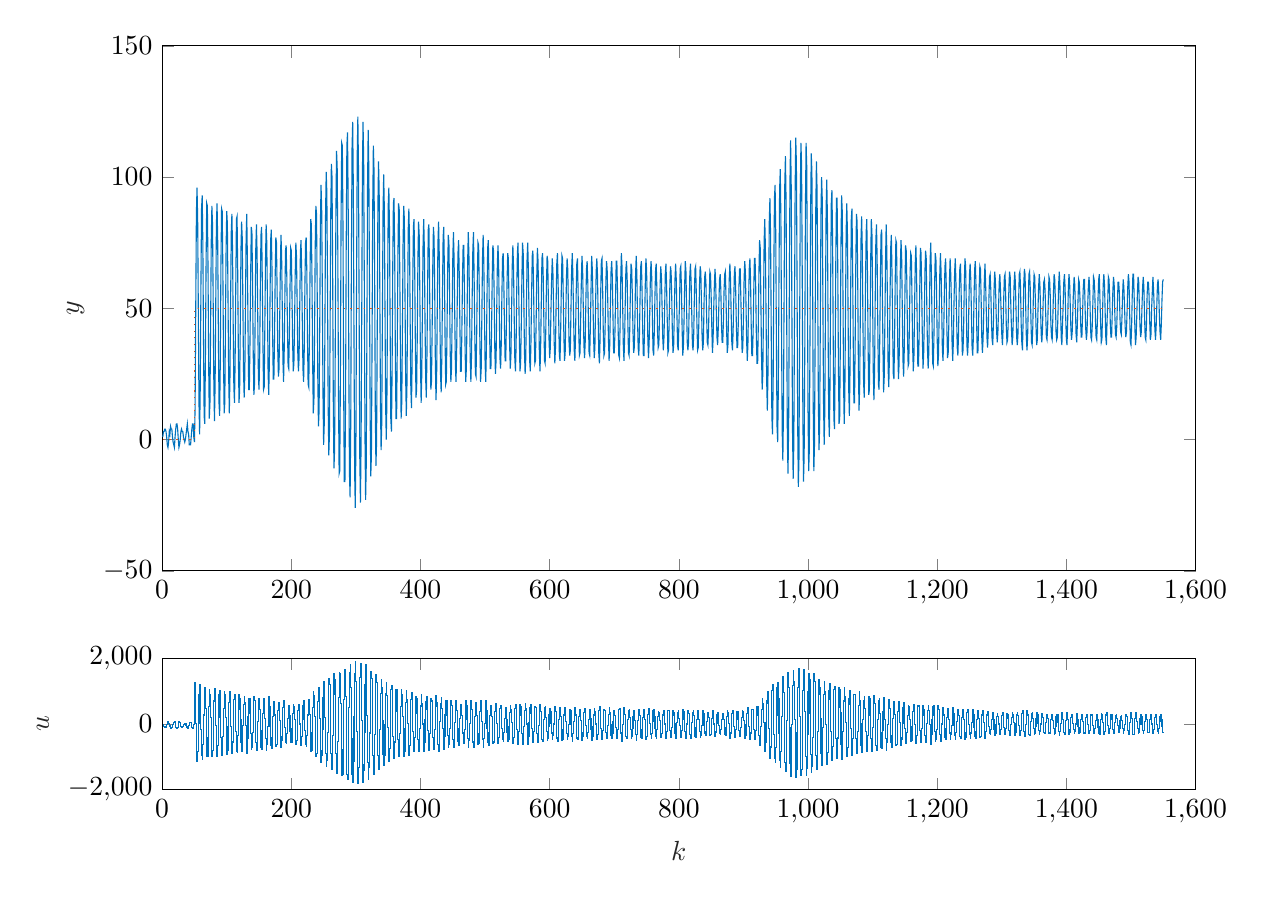
\begin{tikzpicture}

\begin{axis}[%
width=5.167in,
height=0.656in,
at={(0.646in,0.525in)},
scale only axis,
xmin=0,
xmax=1600,
xtick={0,200,400,600,800,1000,1200,1400,1600},
xlabel style={font=\color{white!15!black}},
xlabel={$k$},
ymin=-2000,
ymax=2000,
ytick={-2000,0,2000},
ylabel style={font=\color{white!15!black}},
ylabel={$u$},
axis background/.style={fill=white}
]
\addplot[const plot, color=mycolor1, forget plot] table[row sep=crcr] {%
1	-25\\
2	-75\\
3	-75\\
4	-100\\
5	-100\\
6	-75\\
7	-25\\
8	50\\
9	75\\
10	25\\
11	-75\\
12	-50\\
13	-125\\
14	-100\\
15	-100\\
16	-25\\
17	25\\
18	50\\
19	75\\
20	-25\\
21	-100\\
22	-150\\
23	-150\\
24	-100\\
25	-0\\
26	75\\
27	50\\
28	-0\\
29	-75\\
30	-100\\
31	-75\\
32	-75\\
33	-25\\
34	-0\\
35	25\\
36	-0\\
37	-50\\
38	-100\\
39	-150\\
40	-75\\
41	-50\\
42	50\\
43	50\\
44	50\\
45	-25\\
46	-100\\
47	-150\\
48	-150\\
49	-25\\
50	1275\\
51	950\\
52	25\\
53	-900\\
54	-1150\\
55	-850\\
56	25\\
57	900\\
58	1200\\
59	750\\
60	-175\\
61	-950\\
62	-1075\\
63	-625\\
64	275\\
65	1025\\
66	1100\\
67	475\\
68	-425\\
69	-1000\\
70	-975\\
71	-400\\
72	525\\
73	1050\\
74	900\\
75	200\\
76	-625\\
77	-975\\
78	-800\\
79	-75\\
80	700\\
81	1075\\
82	725\\
83	-50\\
84	-800\\
85	-1000\\
86	-650\\
87	200\\
88	900\\
89	1025\\
90	525\\
91	-400\\
92	-950\\
93	-925\\
94	-375\\
95	475\\
96	1000\\
97	900\\
98	200\\
99	-575\\
100	-925\\
101	-800\\
102	-75\\
103	650\\
104	1000\\
105	650\\
106	-75\\
107	-725\\
108	-900\\
109	-550\\
110	150\\
111	750\\
112	900\\
113	500\\
114	-225\\
115	-850\\
116	-875\\
117	-350\\
118	450\\
119	900\\
120	775\\
121	150\\
122	-550\\
123	-825\\
124	-675\\
125	-50\\
126	600\\
127	850\\
128	650\\
129	-50\\
130	-675\\
131	-900\\
132	-450\\
133	225\\
134	775\\
135	775\\
136	325\\
137	-300\\
138	-775\\
139	-725\\
140	-250\\
141	425\\
142	825\\
143	725\\
144	75\\
145	-575\\
146	-800\\
147	-525\\
148	75\\
149	650\\
150	775\\
151	450\\
152	-200\\
153	-700\\
154	-775\\
155	-300\\
156	325\\
157	775\\
158	750\\
159	175\\
160	-450\\
161	-800\\
162	-625\\
163	-75\\
164	600\\
165	825\\
166	525\\
167	-75\\
168	-650\\
169	-750\\
170	-400\\
171	225\\
172	675\\
173	675\\
174	275\\
175	-300\\
176	-675\\
177	-625\\
178	-175\\
179	400\\
180	650\\
181	575\\
182	100\\
183	-375\\
184	-700\\
185	-500\\
186	-0\\
187	500\\
188	700\\
189	400\\
190	-100\\
191	-550\\
192	-600\\
193	-300\\
194	175\\
195	550\\
196	575\\
197	250\\
198	-225\\
199	-575\\
200	-550\\
201	-150\\
202	325\\
203	600\\
204	525\\
205	150\\
206	-325\\
207	-625\\
208	-500\\
209	-50\\
210	425\\
211	600\\
212	475\\
213	-0\\
214	-525\\
215	-650\\
216	-375\\
217	125\\
218	575\\
219	700\\
220	400\\
221	-200\\
222	-625\\
223	-675\\
224	-350\\
225	275\\
226	725\\
227	750\\
228	300\\
229	-350\\
230	-850\\
231	-800\\
232	-275\\
233	500\\
234	1000\\
235	875\\
236	225\\
237	-600\\
238	-975\\
239	-900\\
240	-200\\
241	675\\
242	1125\\
243	975\\
244	175\\
245	-800\\
246	-1175\\
247	-950\\
248	-175\\
249	800\\
250	1300\\
251	1100\\
252	200\\
253	-900\\
254	-1300\\
255	-1100\\
256	-250\\
257	900\\
258	1400\\
259	1200\\
260	225\\
261	-900\\
262	-1375\\
263	-1250\\
264	-350\\
265	900\\
266	1525\\
267	1350\\
268	400\\
269	-900\\
270	-1500\\
271	-1350\\
272	-525\\
273	800\\
274	1575\\
275	1550\\
276	625\\
277	-850\\
278	-1575\\
279	-1550\\
280	-775\\
281	750\\
282	1650\\
283	1650\\
284	850\\
285	-625\\
286	-1550\\
287	-1675\\
288	-1025\\
289	500\\
290	1575\\
291	1800\\
292	1100\\
293	-450\\
294	-1525\\
295	-1775\\
296	-1150\\
297	225\\
298	1550\\
299	1900\\
300	1300\\
301	-225\\
302	-1450\\
303	-1825\\
304	-1325\\
305	50\\
306	1425\\
307	1850\\
308	1300\\
309	100\\
310	-1250\\
311	-1775\\
312	-1425\\
313	-250\\
314	1200\\
315	1825\\
316	1500\\
317	250\\
318	-1175\\
319	-1700\\
320	-1325\\
321	-275\\
322	1000\\
323	1600\\
324	1400\\
325	325\\
326	-950\\
327	-1550\\
328	-1325\\
329	-325\\
330	975\\
331	1500\\
332	1275\\
333	250\\
334	-950\\
335	-1400\\
336	-1125\\
337	-175\\
338	925\\
339	1350\\
340	1100\\
341	100\\
342	-925\\
343	-1275\\
344	-950\\
345	-25\\
346	925\\
347	1250\\
348	875\\
349	-100\\
350	-975\\
351	-1150\\
352	-750\\
353	200\\
354	1050\\
355	1175\\
356	625\\
357	-375\\
358	-1000\\
359	-1050\\
360	-550\\
361	375\\
362	1050\\
363	1050\\
364	400\\
365	-475\\
366	-1000\\
367	-950\\
368	-300\\
369	525\\
370	1050\\
371	900\\
372	225\\
373	-625\\
374	-975\\
375	-850\\
376	-125\\
377	650\\
378	1025\\
379	750\\
380	25\\
381	-750\\
382	-950\\
383	-650\\
384	125\\
385	750\\
386	950\\
387	525\\
388	-225\\
389	-775\\
390	-850\\
391	-400\\
392	325\\
393	850\\
394	775\\
395	275\\
396	-475\\
397	-825\\
398	-700\\
399	-125\\
400	550\\
401	900\\
402	625\\
403	-0\\
404	-625\\
405	-850\\
406	-550\\
407	125\\
408	675\\
409	850\\
410	450\\
411	-200\\
412	-750\\
413	-800\\
414	-300\\
415	350\\
416	775\\
417	700\\
418	225\\
419	-400\\
420	-775\\
421	-675\\
422	-175\\
423	525\\
424	875\\
425	650\\
426	-0\\
427	-625\\
428	-825\\
429	-525\\
430	75\\
431	625\\
432	800\\
433	475\\
434	-125\\
435	-675\\
436	-775\\
437	-375\\
438	275\\
439	725\\
440	700\\
441	250\\
442	-350\\
443	-700\\
444	-625\\
445	-150\\
446	425\\
447	700\\
448	575\\
449	75\\
450	-475\\
451	-725\\
452	-475\\
453	50\\
454	550\\
455	700\\
456	400\\
457	-125\\
458	-525\\
459	-650\\
460	-325\\
461	175\\
462	600\\
463	600\\
464	250\\
465	-275\\
466	-600\\
467	-600\\
468	-175\\
469	375\\
470	700\\
471	575\\
472	125\\
473	-450\\
474	-725\\
475	-500\\
476	25\\
477	500\\
478	700\\
479	450\\
480	-100\\
481	-550\\
482	-725\\
483	-325\\
484	225\\
485	625\\
486	650\\
487	250\\
488	-300\\
489	-625\\
490	-600\\
491	-175\\
492	375\\
493	700\\
494	575\\
495	75\\
496	-475\\
497	-700\\
498	-450\\
499	25\\
500	525\\
501	700\\
502	400\\
503	-125\\
504	-575\\
505	-650\\
506	-275\\
507	250\\
508	575\\
509	575\\
510	225\\
511	-275\\
512	-600\\
513	-550\\
514	-150\\
515	375\\
516	625\\
517	500\\
518	25\\
519	-425\\
520	-600\\
521	-400\\
522	50\\
523	475\\
524	575\\
525	350\\
526	-125\\
527	-475\\
528	-525\\
529	-250\\
530	175\\
531	500\\
532	500\\
533	150\\
534	-250\\
535	-525\\
536	-475\\
537	-75\\
538	350\\
539	575\\
540	450\\
541	50\\
542	-400\\
543	-600\\
544	-400\\
545	50\\
546	475\\
547	600\\
548	375\\
549	-175\\
550	-525\\
551	-625\\
552	-225\\
553	275\\
554	600\\
555	525\\
556	175\\
557	-300\\
558	-625\\
559	-525\\
560	-75\\
561	425\\
562	625\\
563	475\\
564	-0\\
565	-475\\
566	-625\\
567	-375\\
568	50\\
569	500\\
570	600\\
571	325\\
572	-125\\
573	-500\\
574	-550\\
575	-225\\
576	225\\
577	525\\
578	500\\
579	150\\
580	-300\\
581	-575\\
582	-450\\
583	-50\\
584	425\\
585	600\\
586	375\\
587	-50\\
588	-475\\
589	-525\\
590	-300\\
591	125\\
592	500\\
593	525\\
594	200\\
595	-225\\
596	-500\\
597	-450\\
598	-75\\
599	300\\
600	475\\
601	375\\
602	25\\
603	-275\\
604	-475\\
605	-350\\
606	-0\\
607	325\\
608	525\\
609	375\\
610	-50\\
611	-425\\
612	-525\\
613	-275\\
614	125\\
615	450\\
616	500\\
617	225\\
618	-175\\
619	-500\\
620	-475\\
621	-125\\
622	275\\
623	500\\
624	425\\
625	75\\
626	-300\\
627	-475\\
628	-375\\
629	-25\\
630	325\\
631	450\\
632	400\\
633	-0\\
634	-375\\
635	-525\\
636	-300\\
637	75\\
638	400\\
639	500\\
640	275\\
641	-125\\
642	-425\\
643	-475\\
644	-175\\
645	225\\
646	450\\
647	425\\
648	100\\
649	-250\\
650	-500\\
651	-375\\
652	-25\\
653	350\\
654	475\\
655	325\\
656	-50\\
657	-375\\
658	-450\\
659	-250\\
660	125\\
661	425\\
662	450\\
663	175\\
664	-175\\
665	-500\\
666	-375\\
667	-75\\
668	275\\
669	475\\
670	375\\
671	-0\\
672	-350\\
673	-475\\
674	-325\\
675	50\\
676	425\\
677	525\\
678	300\\
679	-150\\
680	-450\\
681	-475\\
682	-200\\
683	225\\
684	450\\
685	425\\
686	125\\
687	-250\\
688	-450\\
689	-375\\
690	-50\\
691	300\\
692	500\\
693	350\\
694	-25\\
695	-350\\
696	-450\\
697	-300\\
698	75\\
699	425\\
700	425\\
701	250\\
702	-100\\
703	-450\\
704	-450\\
705	-175\\
706	200\\
707	450\\
708	475\\
709	175\\
710	-275\\
711	-525\\
712	-400\\
713	-25\\
714	350\\
715	500\\
716	300\\
717	-50\\
718	-375\\
719	-450\\
720	-275\\
721	125\\
722	425\\
723	450\\
724	200\\
725	-175\\
726	-425\\
727	-375\\
728	-125\\
729	225\\
730	425\\
731	375\\
732	100\\
733	-325\\
734	-500\\
735	-325\\
736	100\\
737	375\\
738	450\\
739	250\\
740	-125\\
741	-400\\
742	-450\\
743	-175\\
744	200\\
745	450\\
746	450\\
747	125\\
748	-225\\
749	-475\\
750	-375\\
751	-75\\
752	300\\
753	475\\
754	325\\
755	25\\
756	-325\\
757	-450\\
758	-300\\
759	75\\
760	400\\
761	450\\
762	225\\
763	-125\\
764	-375\\
765	-425\\
766	-175\\
767	225\\
768	375\\
769	350\\
770	100\\
771	-225\\
772	-400\\
773	-300\\
774	-25\\
775	275\\
776	400\\
777	275\\
778	-0\\
779	-325\\
780	-425\\
781	-225\\
782	100\\
783	425\\
784	400\\
785	125\\
786	-200\\
787	-400\\
788	-350\\
789	-100\\
790	250\\
791	425\\
792	350\\
793	25\\
794	-275\\
795	-425\\
796	-275\\
797	50\\
798	350\\
799	400\\
800	175\\
801	-50\\
802	-375\\
803	-400\\
804	-200\\
805	175\\
806	450\\
807	375\\
808	125\\
809	-225\\
810	-450\\
811	-350\\
812	-0\\
813	325\\
814	400\\
815	325\\
816	-25\\
817	-325\\
818	-425\\
819	-250\\
820	50\\
821	350\\
822	400\\
823	250\\
824	-100\\
825	-375\\
826	-400\\
827	-150\\
828	150\\
829	400\\
830	375\\
831	125\\
832	-225\\
833	-400\\
834	-350\\
835	-50\\
836	275\\
837	400\\
838	325\\
839	-50\\
840	-300\\
841	-350\\
842	-225\\
843	75\\
844	325\\
845	350\\
846	200\\
847	-100\\
848	-350\\
849	-325\\
850	-125\\
851	175\\
852	425\\
853	300\\
854	-0\\
855	-225\\
856	-375\\
857	-250\\
858	25\\
859	275\\
860	350\\
861	200\\
862	-50\\
863	-275\\
864	-325\\
865	-175\\
866	150\\
867	325\\
868	325\\
869	125\\
870	-175\\
871	-325\\
872	-350\\
873	-100\\
874	225\\
875	425\\
876	350\\
877	25\\
878	-275\\
879	-425\\
880	-275\\
881	50\\
882	325\\
883	400\\
884	225\\
885	-75\\
886	-350\\
887	-400\\
888	-175\\
889	150\\
890	375\\
891	375\\
892	150\\
893	-200\\
894	-375\\
895	-375\\
896	-100\\
897	200\\
898	425\\
899	375\\
900	100\\
901	-275\\
902	-450\\
903	-350\\
904	-25\\
905	325\\
906	500\\
907	325\\
908	-75\\
909	-375\\
910	-475\\
911	-275\\
912	150\\
913	450\\
914	450\\
915	225\\
916	-175\\
917	-475\\
918	-475\\
919	-200\\
920	275\\
921	525\\
922	525\\
923	175\\
924	-350\\
925	-650\\
926	-575\\
927	-75\\
928	450\\
929	775\\
930	625\\
931	50\\
932	-625\\
933	-850\\
934	-575\\
935	50\\
936	700\\
937	975\\
938	625\\
939	-125\\
940	-825\\
941	-1050\\
942	-700\\
943	200\\
944	1025\\
945	1200\\
946	725\\
947	-325\\
948	-1050\\
949	-1175\\
950	-725\\
951	275\\
952	1125\\
953	1275\\
954	775\\
955	-275\\
956	-1125\\
957	-1325\\
958	-850\\
959	225\\
960	1175\\
961	1450\\
962	950\\
963	-200\\
964	-1175\\
965	-1450\\
966	-1025\\
967	100\\
968	1250\\
969	1575\\
970	1125\\
971	-100\\
972	-1200\\
973	-1600\\
974	-1150\\
975	-25\\
976	1175\\
977	1625\\
978	1300\\
979	150\\
980	-1125\\
981	-1625\\
982	-1375\\
983	-275\\
984	1125\\
985	1700\\
986	1425\\
987	225\\
988	-1075\\
989	-1575\\
990	-1375\\
991	-375\\
992	1025\\
993	1650\\
994	1400\\
995	375\\
996	-1000\\
997	-1575\\
998	-1350\\
999	-325\\
1000	975\\
1001	1550\\
1002	1350\\
1003	325\\
1004	-925\\
1005	-1475\\
1006	-1300\\
1007	-400\\
1008	900\\
1009	1550\\
1010	1300\\
1011	250\\
1012	-950\\
1013	-1400\\
1014	-1125\\
1015	-225\\
1016	900\\
1017	1350\\
1018	1125\\
1019	175\\
1020	-900\\
1021	-1250\\
1022	-1050\\
1023	-100\\
1024	900\\
1025	1300\\
1026	975\\
1027	-25\\
1028	-950\\
1029	-1225\\
1030	-875\\
1031	125\\
1032	1025\\
1033	1225\\
1034	750\\
1035	-225\\
1036	-1000\\
1037	-1125\\
1038	-675\\
1039	300\\
1040	1050\\
1041	1150\\
1042	525\\
1043	-450\\
1044	-1050\\
1045	-1050\\
1046	-425\\
1047	500\\
1048	1100\\
1049	1050\\
1050	350\\
1051	-625\\
1052	-1075\\
1053	-925\\
1054	-225\\
1055	700\\
1056	1100\\
1057	825\\
1058	50\\
1059	-725\\
1060	-1000\\
1061	-725\\
1062	50\\
1063	775\\
1064	1025\\
1065	600\\
1066	-150\\
1067	-850\\
1068	-950\\
1069	-450\\
1070	325\\
1071	900\\
1072	900\\
1073	325\\
1074	-450\\
1075	-900\\
1076	-825\\
1077	-225\\
1078	575\\
1079	975\\
1080	725\\
1081	25\\
1082	-650\\
1083	-875\\
1084	-575\\
1085	125\\
1086	700\\
1087	850\\
1088	475\\
1089	-225\\
1090	-725\\
1091	-850\\
1092	-350\\
1093	350\\
1094	825\\
1095	775\\
1096	250\\
1097	-450\\
1098	-850\\
1099	-700\\
1100	-100\\
1101	600\\
1102	875\\
1103	625\\
1104	-75\\
1105	-650\\
1106	-800\\
1107	-475\\
1108	150\\
1109	725\\
1110	775\\
1111	325\\
1112	-275\\
1113	-700\\
1114	-750\\
1115	-200\\
1116	375\\
1117	800\\
1118	650\\
1119	125\\
1120	-450\\
1121	-800\\
1122	-550\\
1123	-25\\
1124	575\\
1125	750\\
1126	475\\
1127	-125\\
1128	-575\\
1129	-700\\
1130	-350\\
1131	175\\
1132	625\\
1133	675\\
1134	300\\
1135	-275\\
1136	-650\\
1137	-625\\
1138	-150\\
1139	375\\
1140	675\\
1141	525\\
1142	50\\
1143	-425\\
1144	-650\\
1145	-475\\
1146	25\\
1147	500\\
1148	650\\
1149	400\\
1150	-125\\
1151	-600\\
1152	-550\\
1153	-250\\
1154	250\\
1155	550\\
1156	525\\
1157	150\\
1158	-325\\
1159	-525\\
1160	-500\\
1161	-75\\
1162	375\\
1163	600\\
1164	450\\
1165	-25\\
1166	-425\\
1167	-600\\
1168	-350\\
1169	125\\
1170	550\\
1171	550\\
1172	275\\
1173	-200\\
1174	-575\\
1175	-525\\
1176	-150\\
1177	275\\
1178	575\\
1179	450\\
1180	125\\
1181	-350\\
1182	-550\\
1183	-475\\
1184	25\\
1185	400\\
1186	575\\
1187	425\\
1188	-25\\
1189	-450\\
1190	-625\\
1191	-325\\
1192	125\\
1193	525\\
1194	550\\
1195	250\\
1196	-225\\
1197	-525\\
1198	-475\\
1199	-175\\
1200	300\\
1201	550\\
1202	450\\
1203	75\\
1204	-325\\
1205	-525\\
1206	-350\\
1207	-0\\
1208	400\\
1209	500\\
1210	275\\
1211	-125\\
1212	-400\\
1213	-475\\
1214	-225\\
1215	200\\
1216	475\\
1217	425\\
1218	150\\
1219	-275\\
1220	-475\\
1221	-325\\
1222	-50\\
1223	325\\
1224	500\\
1225	325\\
1226	-50\\
1227	-350\\
1228	-475\\
1229	-250\\
1230	75\\
1231	375\\
1232	450\\
1233	250\\
1234	-150\\
1235	-375\\
1236	-425\\
1237	-175\\
1238	200\\
1239	450\\
1240	400\\
1241	150\\
1242	-250\\
1243	-475\\
1244	-400\\
1245	-50\\
1246	350\\
1247	450\\
1248	325\\
1249	-25\\
1250	-325\\
1251	-425\\
1252	-275\\
1253	50\\
1254	375\\
1255	450\\
1256	275\\
1257	-100\\
1258	-375\\
1259	-450\\
1260	-225\\
1261	125\\
1262	425\\
1263	425\\
1264	175\\
1265	-200\\
1266	-400\\
1267	-375\\
1268	-100\\
1269	275\\
1270	425\\
1271	300\\
1272	50\\
1273	-275\\
1274	-425\\
1275	-225\\
1276	25\\
1277	275\\
1278	375\\
1279	225\\
1280	-75\\
1281	-300\\
1282	-325\\
1283	-175\\
1284	125\\
1285	300\\
1286	350\\
1287	150\\
1288	-175\\
1289	-350\\
1290	-275\\
1291	-25\\
1292	225\\
1293	325\\
1294	225\\
1295	-0\\
1296	-250\\
1297	-325\\
1298	-175\\
1299	50\\
1300	250\\
1301	350\\
1302	200\\
1303	-100\\
1304	-300\\
1305	-325\\
1306	-125\\
1307	175\\
1308	325\\
1309	300\\
1310	125\\
1311	-200\\
1312	-350\\
1313	-300\\
1314	-25\\
1315	200\\
1316	350\\
1317	275\\
1318	50\\
1319	-225\\
1320	-350\\
1321	-250\\
1322	-0\\
1323	275\\
1324	350\\
1325	250\\
1326	-50\\
1327	-325\\
1328	-350\\
1329	-200\\
1330	150\\
1331	325\\
1332	400\\
1333	125\\
1334	-225\\
1335	-375\\
1336	-325\\
1337	-25\\
1338	275\\
1339	400\\
1340	275\\
1341	-25\\
1342	-325\\
1343	-350\\
1344	-200\\
1345	75\\
1346	325\\
1347	350\\
1348	175\\
1349	-150\\
1350	-325\\
1351	-300\\
1352	-75\\
1353	175\\
1354	350\\
1355	300\\
1356	25\\
1357	-200\\
1358	-325\\
1359	-225\\
1360	-0\\
1361	250\\
1362	325\\
1363	200\\
1364	-50\\
1365	-250\\
1366	-275\\
1367	-175\\
1368	50\\
1369	275\\
1370	300\\
1371	175\\
1372	-75\\
1373	-300\\
1374	-275\\
1375	-125\\
1376	150\\
1377	275\\
1378	300\\
1379	100\\
1380	-150\\
1381	-325\\
1382	-275\\
1383	-75\\
1384	225\\
1385	300\\
1386	275\\
1387	50\\
1388	-225\\
1389	-350\\
1390	-225\\
1391	25\\
1392	275\\
1393	350\\
1394	150\\
1395	-25\\
1396	-250\\
1397	-325\\
1398	-200\\
1399	100\\
1400	300\\
1401	350\\
1402	125\\
1403	-175\\
1404	-325\\
1405	-250\\
1406	-25\\
1407	200\\
1408	300\\
1409	225\\
1410	25\\
1411	-175\\
1412	-300\\
1413	-225\\
1414	-0\\
1415	250\\
1416	325\\
1417	150\\
1418	-75\\
1419	-275\\
1420	-250\\
1421	-100\\
1422	125\\
1423	275\\
1424	275\\
1425	75\\
1426	-175\\
1427	-275\\
1428	-275\\
1429	-0\\
1430	200\\
1431	300\\
1432	225\\
1433	-25\\
1434	-200\\
1435	-300\\
1436	-200\\
1437	75\\
1438	275\\
1439	300\\
1440	175\\
1441	-50\\
1442	-300\\
1443	-275\\
1444	-150\\
1445	100\\
1446	275\\
1447	300\\
1448	125\\
1449	-100\\
1450	-275\\
1451	-325\\
1452	-75\\
1453	150\\
1454	325\\
1455	300\\
1456	50\\
1457	-225\\
1458	-325\\
1459	-225\\
1460	25\\
1461	275\\
1462	350\\
1463	125\\
1464	-50\\
1465	-300\\
1466	-275\\
1467	-125\\
1468	150\\
1469	275\\
1470	275\\
1471	50\\
1472	-175\\
1473	-300\\
1474	-225\\
1475	50\\
1476	250\\
1477	275\\
1478	175\\
1479	-50\\
1480	-250\\
1481	-250\\
1482	-150\\
1483	100\\
1484	225\\
1485	250\\
1486	100\\
1487	-125\\
1488	-275\\
1489	-200\\
1490	-25\\
1491	175\\
1492	275\\
1493	225\\
1494	25\\
1495	-200\\
1496	-325\\
1497	-250\\
1498	50\\
1499	325\\
1500	350\\
1501	175\\
1502	-125\\
1503	-325\\
1504	-325\\
1505	-100\\
1506	175\\
1507	350\\
1508	275\\
1509	75\\
1510	-150\\
1511	-300\\
1512	-250\\
1513	-25\\
1514	175\\
1515	275\\
1516	225\\
1517	-0\\
1518	-200\\
1519	-300\\
1520	-200\\
1521	75\\
1522	275\\
1523	300\\
1524	150\\
1525	-125\\
1526	-250\\
1527	-250\\
1528	-125\\
1529	125\\
1530	300\\
1531	250\\
1532	-0\\
1533	-150\\
1534	-300\\
1535	-175\\
1536	-0\\
1537	200\\
1538	300\\
1539	175\\
1540	-25\\
1541	-225\\
1542	-275\\
1543	-150\\
1544	75\\
1545	225\\
1546	300\\
1547	150\\
1548	-75\\
1549	-250\\
1550	-275\\
};
\end{axis}

\begin{axis}[%
width=5.167in,
height=2.625in,
at={(0.646in,1.619in)},
scale only axis,
xmin=0,
xmax=1600,
xtick={0,200,400,600,800,1000,1200,1400,1600},
ymin=-50,
ymax=150,
ytick={-50,0,50,100,150},
ylabel style={font=\color{white!15!black}},
ylabel={$y$},
axis background/.style={fill=white}
]
\addplot [color=mycolor1, forget plot]
  table[row sep=crcr]{%
1	1\\
2	3\\
3	3\\
4	4\\
5	4\\
6	3\\
7	1\\
8	-2\\
9	-3\\
10	-1\\
11	3\\
12	2\\
13	5\\
14	4\\
15	4\\
16	1\\
17	-1\\
18	-2\\
19	-3\\
20	1\\
21	4\\
22	6\\
23	6\\
24	4\\
25	0\\
26	-3\\
27	-2\\
28	0\\
29	3\\
30	4\\
31	3\\
32	3\\
33	1\\
34	0\\
35	-1\\
36	0\\
37	2\\
38	4\\
39	6\\
40	3\\
41	2\\
42	-2\\
43	-2\\
44	-2\\
45	1\\
46	4\\
47	6\\
48	6\\
49	1\\
50	-1\\
51	12\\
52	49\\
53	86\\
54	96\\
55	84\\
56	49\\
57	14\\
58	2\\
59	20\\
60	57\\
61	88\\
62	93\\
63	75\\
64	39\\
65	9\\
66	6\\
67	31\\
68	67\\
69	90\\
70	89\\
71	66\\
72	29\\
73	8\\
74	14\\
75	42\\
76	75\\
77	89\\
78	82\\
79	53\\
80	22\\
81	7\\
82	21\\
83	52\\
84	82\\
85	90\\
86	76\\
87	42\\
88	14\\
89	9\\
90	29\\
91	66\\
92	88\\
93	87\\
94	65\\
95	31\\
96	10\\
97	14\\
98	42\\
99	73\\
100	87\\
101	82\\
102	53\\
103	24\\
104	10\\
105	24\\
106	53\\
107	79\\
108	86\\
109	72\\
110	44\\
111	20\\
112	14\\
113	30\\
114	59\\
115	84\\
116	85\\
117	64\\
118	32\\
119	14\\
120	19\\
121	44\\
122	72\\
123	83\\
124	77\\
125	52\\
126	26\\
127	16\\
128	24\\
129	52\\
130	77\\
131	86\\
132	68\\
133	41\\
134	19\\
135	19\\
136	37\\
137	62\\
138	81\\
139	79\\
140	60\\
141	33\\
142	17\\
143	21\\
144	47\\
145	73\\
146	82\\
147	71\\
148	47\\
149	24\\
150	19\\
151	32\\
152	58\\
153	78\\
154	81\\
155	62\\
156	37\\
157	19\\
158	20\\
159	43\\
160	68\\
161	82\\
162	75\\
163	53\\
164	26\\
165	17\\
166	29\\
167	53\\
168	76\\
169	80\\
170	66\\
171	41\\
172	23\\
173	23\\
174	39\\
175	62\\
176	77\\
177	75\\
178	57\\
179	34\\
180	24\\
181	27\\
182	46\\
183	65\\
184	78\\
185	70\\
186	50\\
187	30\\
188	22\\
189	34\\
190	54\\
191	72\\
192	74\\
193	62\\
194	43\\
195	28\\
196	27\\
197	40\\
198	59\\
199	73\\
200	72\\
201	56\\
202	37\\
203	26\\
204	29\\
205	44\\
206	63\\
207	75\\
208	70\\
209	52\\
210	33\\
211	26\\
212	31\\
213	50\\
214	71\\
215	76\\
216	65\\
217	45\\
218	27\\
219	22\\
220	34\\
221	58\\
222	75\\
223	77\\
224	64\\
225	39\\
226	21\\
227	20\\
228	38\\
229	64\\
230	84\\
231	82\\
232	61\\
233	30\\
234	10\\
235	15\\
236	41\\
237	74\\
238	89\\
239	86\\
240	58\\
241	23\\
242	5\\
243	11\\
244	43\\
245	82\\
246	97\\
247	88\\
248	57\\
249	18\\
250	-2\\
251	6\\
252	42\\
253	86\\
254	102\\
255	94\\
256	60\\
257	14\\
258	-6\\
259	2\\
260	41\\
261	86\\
262	105\\
263	100\\
264	64\\
265	14\\
266	-11\\
267	-4\\
268	34\\
269	86\\
270	110\\
271	104\\
272	71\\
273	18\\
274	-13\\
275	-12\\
276	25\\
277	84\\
278	113\\
279	112\\
280	81\\
281	20\\
282	-16\\
283	-16\\
284	16\\
285	75\\
286	112\\
287	117\\
288	91\\
289	30\\
290	-13\\
291	-22\\
292	6\\
293	68\\
294	111\\
295	121\\
296	96\\
297	41\\
298	-12\\
299	-26\\
300	-2\\
301	59\\
302	108\\
303	123\\
304	103\\
305	48\\
306	-7\\
307	-24\\
308	-2\\
309	46\\
310	100\\
311	121\\
312	107\\
313	60\\
314	2\\
315	-23\\
316	-10\\
317	40\\
318	97\\
319	118\\
320	103\\
321	61\\
322	10\\
323	-14\\
324	-6\\
325	37\\
326	88\\
327	112\\
328	103\\
329	63\\
330	11\\
331	-10\\
332	-1\\
333	40\\
334	88\\
335	106\\
336	95\\
337	57\\
338	13\\
339	-4\\
340	6\\
341	46\\
342	87\\
343	101\\
344	88\\
345	51\\
346	13\\
347	0\\
348	15\\
349	54\\
350	89\\
351	96\\
352	80\\
353	42\\
354	8\\
355	3\\
356	25\\
357	65\\
358	90\\
359	92\\
360	72\\
361	35\\
362	8\\
363	8\\
364	34\\
365	69\\
366	90\\
367	88\\
368	62\\
369	29\\
370	8\\
371	14\\
372	41\\
373	75\\
374	89\\
375	84\\
376	55\\
377	24\\
378	9\\
379	20\\
380	49\\
381	80\\
382	88\\
383	76\\
384	45\\
385	20\\
386	12\\
387	29\\
388	59\\
389	81\\
390	84\\
391	66\\
392	37\\
393	16\\
394	19\\
395	39\\
396	69\\
397	83\\
398	78\\
399	55\\
400	28\\
401	14\\
402	25\\
403	50\\
404	75\\
405	84\\
406	72\\
407	45\\
408	23\\
409	16\\
410	32\\
411	58\\
412	80\\
413	82\\
414	62\\
415	36\\
416	19\\
417	22\\
418	41\\
419	66\\
420	81\\
421	77\\
422	57\\
423	29\\
424	15\\
425	24\\
426	50\\
427	75\\
428	83\\
429	71\\
430	47\\
431	25\\
432	18\\
433	31\\
434	55\\
435	77\\
436	81\\
437	65\\
438	39\\
439	21\\
440	22\\
441	40\\
442	64\\
443	78\\
444	75\\
445	56\\
446	33\\
447	22\\
448	27\\
449	47\\
450	69\\
451	79\\
452	69\\
453	48\\
454	28\\
455	22\\
456	34\\
457	55\\
458	71\\
459	76\\
460	63\\
461	43\\
462	26\\
463	26\\
464	40\\
465	61\\
466	74\\
467	74\\
468	57\\
469	35\\
470	22\\
471	27\\
472	45\\
473	68\\
474	79\\
475	70\\
476	49\\
477	30\\
478	22\\
479	32\\
480	54\\
481	72\\
482	79\\
483	63\\
484	41\\
485	25\\
486	24\\
487	40\\
488	62\\
489	75\\
490	74\\
491	57\\
492	35\\
493	22\\
494	27\\
495	47\\
496	69\\
497	78\\
498	68\\
499	49\\
500	29\\
501	22\\
502	34\\
503	55\\
504	73\\
505	76\\
506	61\\
507	40\\
508	27\\
509	27\\
510	41\\
511	61\\
512	74\\
513	72\\
514	56\\
515	35\\
516	25\\
517	30\\
518	49\\
519	67\\
520	74\\
521	66\\
522	48\\
523	31\\
524	27\\
525	36\\
526	55\\
527	69\\
528	71\\
529	60\\
530	43\\
531	30\\
532	30\\
533	44\\
534	60\\
535	71\\
536	69\\
537	53\\
538	36\\
539	27\\
540	32\\
541	48\\
542	66\\
543	74\\
544	66\\
545	48\\
546	31\\
547	26\\
548	35\\
549	57\\
550	71\\
551	75\\
552	59\\
553	39\\
554	26\\
555	29\\
556	43\\
557	62\\
558	75\\
559	71\\
560	53\\
561	33\\
562	25\\
563	31\\
564	50\\
565	69\\
566	75\\
567	65\\
568	48\\
569	30\\
570	26\\
571	37\\
572	55\\
573	70\\
574	72\\
575	59\\
576	41\\
577	29\\
578	30\\
579	44\\
580	62\\
581	73\\
582	68\\
583	52\\
584	33\\
585	26\\
586	35\\
587	52\\
588	69\\
589	71\\
590	62\\
591	45\\
592	30\\
593	29\\
594	42\\
595	59\\
596	70\\
597	68\\
598	53\\
599	38\\
600	31\\
601	35\\
602	49\\
603	61\\
604	69\\
605	64\\
606	50\\
607	37\\
608	29\\
609	35\\
610	52\\
611	67\\
612	71\\
613	61\\
614	45\\
615	32\\
616	30\\
617	41\\
618	57\\
619	70\\
620	69\\
621	55\\
622	39\\
623	30\\
624	33\\
625	47\\
626	62\\
627	69\\
628	65\\
629	51\\
630	37\\
631	32\\
632	34\\
633	50\\
634	65\\
635	71\\
636	62\\
637	47\\
638	34\\
639	30\\
640	39\\
641	55\\
642	67\\
643	69\\
644	57\\
645	41\\
646	32\\
647	33\\
648	46\\
649	60\\
650	70\\
651	65\\
652	51\\
653	36\\
654	31\\
655	37\\
656	52\\
657	65\\
658	68\\
659	60\\
660	45\\
661	33\\
662	32\\
663	43\\
664	57\\
665	70\\
666	65\\
667	53\\
668	39\\
669	31\\
670	35\\
671	50\\
672	64\\
673	69\\
674	63\\
675	48\\
676	33\\
677	29\\
678	38\\
679	56\\
680	68\\
681	69\\
682	58\\
683	41\\
684	32\\
685	33\\
686	45\\
687	60\\
688	68\\
689	65\\
690	52\\
691	38\\
692	30\\
693	36\\
694	51\\
695	64\\
696	68\\
697	62\\
698	47\\
699	33\\
700	33\\
701	40\\
702	54\\
703	68\\
704	68\\
705	57\\
706	42\\
707	32\\
708	31\\
709	43\\
710	61\\
711	71\\
712	66\\
713	51\\
714	36\\
715	30\\
716	38\\
717	52\\
718	65\\
719	68\\
720	61\\
721	45\\
722	33\\
723	32\\
724	42\\
725	57\\
726	67\\
727	65\\
728	55\\
729	41\\
730	33\\
731	35\\
732	46\\
733	63\\
734	70\\
735	63\\
736	46\\
737	35\\
738	32\\
739	40\\
740	55\\
741	66\\
742	68\\
743	57\\
744	42\\
745	32\\
746	32\\
747	45\\
748	59\\
749	69\\
750	65\\
751	53\\
752	38\\
753	31\\
754	37\\
755	49\\
756	63\\
757	68\\
758	62\\
759	47\\
760	34\\
761	32\\
762	41\\
763	55\\
764	65\\
765	67\\
766	57\\
767	41\\
768	35\\
769	36\\
770	46\\
771	59\\
772	66\\
773	62\\
774	51\\
775	39\\
776	34\\
777	39\\
778	50\\
779	63\\
780	67\\
781	59\\
782	46\\
783	33\\
784	34\\
785	45\\
786	58\\
787	66\\
788	64\\
789	54\\
790	40\\
791	33\\
792	36\\
793	49\\
794	61\\
795	67\\
796	61\\
797	48\\
798	36\\
799	34\\
800	43\\
801	52\\
802	65\\
803	66\\
804	58\\
805	43\\
806	32\\
807	35\\
808	45\\
809	59\\
810	68\\
811	64\\
812	50\\
813	37\\
814	34\\
815	37\\
816	51\\
817	63\\
818	67\\
819	60\\
820	48\\
821	36\\
822	34\\
823	40\\
824	54\\
825	65\\
826	66\\
827	56\\
828	44\\
829	34\\
830	35\\
831	45\\
832	59\\
833	66\\
834	64\\
835	52\\
836	39\\
837	34\\
838	37\\
839	52\\
840	62\\
841	64\\
842	59\\
843	47\\
844	37\\
845	36\\
846	42\\
847	54\\
848	64\\
849	63\\
850	55\\
851	43\\
852	33\\
853	38\\
854	50\\
855	59\\
856	65\\
857	60\\
858	49\\
859	39\\
860	36\\
861	42\\
862	52\\
863	61\\
864	63\\
865	57\\
866	44\\
867	37\\
868	37\\
869	45\\
870	57\\
871	63\\
872	64\\
873	54\\
874	41\\
875	33\\
876	36\\
877	49\\
878	61\\
879	67\\
880	61\\
881	48\\
882	37\\
883	34\\
884	41\\
885	53\\
886	64\\
887	66\\
888	57\\
889	44\\
890	35\\
891	35\\
892	44\\
893	58\\
894	65\\
895	65\\
896	54\\
897	42\\
898	33\\
899	35\\
900	46\\
901	61\\
902	68\\
903	64\\
904	51\\
905	37\\
906	30\\
907	37\\
908	53\\
909	65\\
910	69\\
911	61\\
912	44\\
913	32\\
914	32\\
915	41\\
916	57\\
917	69\\
918	69\\
919	58\\
920	39\\
921	29\\
922	29\\
923	43\\
924	64\\
925	76\\
926	73\\
927	53\\
928	32\\
929	19\\
930	25\\
931	48\\
932	75\\
933	84\\
934	73\\
935	48\\
936	22\\
937	11\\
938	25\\
939	55\\
940	83\\
941	92\\
942	78\\
943	42\\
944	9\\
945	2\\
946	21\\
947	63\\
948	92\\
949	97\\
950	79\\
951	39\\
952	5\\
953	-1\\
954	19\\
955	61\\
956	95\\
957	103\\
958	84\\
959	41\\
960	3\\
961	-8\\
962	12\\
963	58\\
964	97\\
965	108\\
966	91\\
967	46\\
968	0\\
969	-13\\
970	5\\
971	54\\
972	98\\
973	114\\
974	96\\
975	51\\
976	3\\
977	-15\\
978	-2\\
979	44\\
980	95\\
981	115\\
982	105\\
983	61\\
984	5\\
985	-18\\
986	-7\\
987	41\\
988	93\\
989	113\\
990	105\\
991	65\\
992	9\\
993	-16\\
994	-6\\
995	35\\
996	90\\
997	113\\
998	104\\
999	63\\
1000	11\\
1001	-12\\
1002	-4\\
1003	37\\
1004	87\\
1005	109\\
1006	102\\
1007	66\\
1008	14\\
1009	-12\\
1010	-2\\
1011	40\\
1012	88\\
1013	106\\
1014	95\\
1015	59\\
1016	14\\
1017	-4\\
1018	5\\
1019	43\\
1020	86\\
1021	100\\
1022	92\\
1023	54\\
1024	14\\
1025	-2\\
1026	11\\
1027	51\\
1028	88\\
1029	99\\
1030	85\\
1031	45\\
1032	9\\
1033	1\\
1034	20\\
1035	59\\
1036	90\\
1037	95\\
1038	77\\
1039	38\\
1040	8\\
1041	4\\
1042	29\\
1043	68\\
1044	92\\
1045	92\\
1046	67\\
1047	30\\
1048	6\\
1049	8\\
1050	36\\
1051	75\\
1052	93\\
1053	87\\
1054	59\\
1055	22\\
1056	6\\
1057	17\\
1058	48\\
1059	79\\
1060	90\\
1061	79\\
1062	48\\
1063	19\\
1064	9\\
1065	26\\
1066	56\\
1067	84\\
1068	88\\
1069	68\\
1070	37\\
1071	14\\
1072	14\\
1073	37\\
1074	68\\
1075	86\\
1076	83\\
1077	59\\
1078	27\\
1079	11\\
1080	21\\
1081	49\\
1082	76\\
1083	85\\
1084	73\\
1085	45\\
1086	22\\
1087	16\\
1088	31\\
1089	59\\
1090	79\\
1091	84\\
1092	64\\
1093	36\\
1094	17\\
1095	19\\
1096	40\\
1097	68\\
1098	84\\
1099	78\\
1100	54\\
1101	26\\
1102	15\\
1103	25\\
1104	53\\
1105	76\\
1106	82\\
1107	69\\
1108	44\\
1109	21\\
1110	19\\
1111	37\\
1112	61\\
1113	78\\
1114	80\\
1115	58\\
1116	35\\
1117	18\\
1118	24\\
1119	45\\
1120	68\\
1121	82\\
1122	72\\
1123	51\\
1124	27\\
1125	20\\
1126	31\\
1127	55\\
1128	73\\
1129	78\\
1130	64\\
1131	43\\
1132	25\\
1133	23\\
1134	38\\
1135	61\\
1136	76\\
1137	75\\
1138	56\\
1139	35\\
1140	23\\
1141	29\\
1142	48\\
1143	67\\
1144	76\\
1145	69\\
1146	49\\
1147	30\\
1148	24\\
1149	34\\
1150	55\\
1151	74\\
1152	72\\
1153	60\\
1154	40\\
1155	28\\
1156	29\\
1157	44\\
1158	63\\
1159	71\\
1160	70\\
1161	53\\
1162	35\\
1163	26\\
1164	32\\
1165	51\\
1166	67\\
1167	74\\
1168	64\\
1169	45\\
1170	28\\
1171	28\\
1172	39\\
1173	58\\
1174	73\\
1175	71\\
1176	56\\
1177	39\\
1178	27\\
1179	32\\
1180	45\\
1181	64\\
1182	72\\
1183	69\\
1184	49\\
1185	34\\
1186	27\\
1187	33\\
1188	51\\
1189	68\\
1190	75\\
1191	63\\
1192	45\\
1193	29\\
1194	28\\
1195	40\\
1196	59\\
1197	71\\
1198	69\\
1199	57\\
1200	38\\
1201	28\\
1202	32\\
1203	47\\
1204	63\\
1205	71\\
1206	64\\
1207	50\\
1208	34\\
1209	30\\
1210	39\\
1211	55\\
1212	66\\
1213	69\\
1214	59\\
1215	42\\
1216	31\\
1217	33\\
1218	44\\
1219	61\\
1220	69\\
1221	63\\
1222	52\\
1223	37\\
1224	30\\
1225	37\\
1226	52\\
1227	64\\
1228	69\\
1229	60\\
1230	47\\
1231	35\\
1232	32\\
1233	40\\
1234	56\\
1235	65\\
1236	67\\
1237	57\\
1238	42\\
1239	32\\
1240	34\\
1241	44\\
1242	60\\
1243	69\\
1244	66\\
1245	52\\
1246	36\\
1247	32\\
1248	37\\
1249	51\\
1250	63\\
1251	67\\
1252	61\\
1253	48\\
1254	35\\
1255	32\\
1256	39\\
1257	54\\
1258	65\\
1259	68\\
1260	59\\
1261	45\\
1262	33\\
1263	33\\
1264	43\\
1265	58\\
1266	66\\
1267	65\\
1268	54\\
1269	39\\
1270	33\\
1271	38\\
1272	48\\
1273	61\\
1274	67\\
1275	59\\
1276	49\\
1277	39\\
1278	35\\
1279	41\\
1280	53\\
1281	62\\
1282	63\\
1283	57\\
1284	45\\
1285	38\\
1286	36\\
1287	44\\
1288	57\\
1289	64\\
1290	61\\
1291	51\\
1292	41\\
1293	37\\
1294	41\\
1295	50\\
1296	60\\
1297	63\\
1298	57\\
1299	48\\
1300	40\\
1301	36\\
1302	42\\
1303	54\\
1304	62\\
1305	63\\
1306	55\\
1307	43\\
1308	37\\
1309	38\\
1310	45\\
1311	58\\
1312	64\\
1313	62\\
1314	51\\
1315	42\\
1316	36\\
1317	39\\
1318	48\\
1319	59\\
1320	64\\
1321	60\\
1322	50\\
1323	39\\
1324	36\\
1325	40\\
1326	52\\
1327	63\\
1328	64\\
1329	58\\
1330	44\\
1331	37\\
1332	34\\
1333	45\\
1334	59\\
1335	65\\
1336	63\\
1337	51\\
1338	39\\
1339	34\\
1340	39\\
1341	51\\
1342	63\\
1343	64\\
1344	58\\
1345	47\\
1346	37\\
1347	36\\
1348	43\\
1349	56\\
1350	63\\
1351	62\\
1352	53\\
1353	43\\
1354	36\\
1355	38\\
1356	49\\
1357	58\\
1358	63\\
1359	59\\
1360	50\\
1361	40\\
1362	37\\
1363	42\\
1364	52\\
1365	60\\
1366	61\\
1367	57\\
1368	48\\
1369	39\\
1370	38\\
1371	43\\
1372	53\\
1373	62\\
1374	61\\
1375	55\\
1376	44\\
1377	39\\
1378	38\\
1379	46\\
1380	56\\
1381	63\\
1382	61\\
1383	53\\
1384	41\\
1385	38\\
1386	39\\
1387	48\\
1388	59\\
1389	64\\
1390	59\\
1391	49\\
1392	39\\
1393	36\\
1394	44\\
1395	51\\
1396	60\\
1397	63\\
1398	58\\
1399	46\\
1400	38\\
1401	36\\
1402	45\\
1403	57\\
1404	63\\
1405	60\\
1406	51\\
1407	42\\
1408	38\\
1409	41\\
1410	49\\
1411	57\\
1412	62\\
1413	59\\
1414	50\\
1415	40\\
1416	37\\
1417	44\\
1418	53\\
1419	61\\
1420	60\\
1421	54\\
1422	45\\
1423	39\\
1424	39\\
1425	47\\
1426	57\\
1427	61\\
1428	61\\
1429	50\\
1430	42\\
1431	38\\
1432	41\\
1433	51\\
1434	58\\
1435	62\\
1436	58\\
1437	47\\
1438	39\\
1439	38\\
1440	43\\
1441	52\\
1442	62\\
1443	61\\
1444	56\\
1445	46\\
1446	39\\
1447	38\\
1448	45\\
1449	54\\
1450	61\\
1451	63\\
1452	53\\
1453	44\\
1454	37\\
1455	38\\
1456	48\\
1457	59\\
1458	63\\
1459	59\\
1460	49\\
1461	39\\
1462	36\\
1463	45\\
1464	52\\
1465	62\\
1466	61\\
1467	55\\
1468	44\\
1469	39\\
1470	39\\
1471	48\\
1472	57\\
1473	62\\
1474	59\\
1475	48\\
1476	40\\
1477	39\\
1478	43\\
1479	52\\
1480	60\\
1481	60\\
1482	56\\
1483	46\\
1484	41\\
1485	40\\
1486	46\\
1487	55\\
1488	61\\
1489	58\\
1490	51\\
1491	43\\
1492	39\\
1493	41\\
1494	49\\
1495	58\\
1496	63\\
1497	60\\
1498	48\\
1499	37\\
1500	36\\
1501	43\\
1502	55\\
1503	63\\
1504	63\\
1505	54\\
1506	43\\
1507	36\\
1508	39\\
1509	47\\
1510	56\\
1511	62\\
1512	60\\
1513	51\\
1514	43\\
1515	39\\
1516	41\\
1517	50\\
1518	58\\
1519	62\\
1520	58\\
1521	47\\
1522	39\\
1523	38\\
1524	44\\
1525	55\\
1526	60\\
1527	60\\
1528	55\\
1529	45\\
1530	38\\
1531	40\\
1532	50\\
1533	56\\
1534	62\\
1535	57\\
1536	50\\
1537	42\\
1538	38\\
1539	43\\
1540	51\\
1541	59\\
1542	61\\
1543	56\\
1544	47\\
1545	41\\
1546	38\\
1547	44\\
1548	53\\
1549	60\\
1550	61\\
};
\addplot[const plot, color=mycolor2, dotted, forget plot] table[row sep=crcr] {%
1	0\\
2	0\\
3	0\\
4	0\\
5	0\\
6	0\\
7	0\\
8	0\\
9	0\\
10	0\\
11	0\\
12	0\\
13	0\\
14	0\\
15	0\\
16	0\\
17	0\\
18	0\\
19	0\\
20	0\\
21	0\\
22	0\\
23	0\\
24	0\\
25	0\\
26	0\\
27	0\\
28	0\\
29	0\\
30	0\\
31	0\\
32	0\\
33	0\\
34	0\\
35	0\\
36	0\\
37	0\\
38	0\\
39	0\\
40	0\\
41	0\\
42	0\\
43	0\\
44	0\\
45	0\\
46	0\\
47	0\\
48	0\\
49	0\\
50	50\\
51	50\\
52	50\\
53	50\\
54	50\\
55	50\\
56	50\\
57	50\\
58	50\\
59	50\\
60	50\\
61	50\\
62	50\\
63	50\\
64	50\\
65	50\\
66	50\\
67	50\\
68	50\\
69	50\\
70	50\\
71	50\\
72	50\\
73	50\\
74	50\\
75	50\\
76	50\\
77	50\\
78	50\\
79	50\\
80	50\\
81	50\\
82	50\\
83	50\\
84	50\\
85	50\\
86	50\\
87	50\\
88	50\\
89	50\\
90	50\\
91	50\\
92	50\\
93	50\\
94	50\\
95	50\\
96	50\\
97	50\\
98	50\\
99	50\\
100	50\\
101	50\\
102	50\\
103	50\\
104	50\\
105	50\\
106	50\\
107	50\\
108	50\\
109	50\\
110	50\\
111	50\\
112	50\\
113	50\\
114	50\\
115	50\\
116	50\\
117	50\\
118	50\\
119	50\\
120	50\\
121	50\\
122	50\\
123	50\\
124	50\\
125	50\\
126	50\\
127	50\\
128	50\\
129	50\\
130	50\\
131	50\\
132	50\\
133	50\\
134	50\\
135	50\\
136	50\\
137	50\\
138	50\\
139	50\\
140	50\\
141	50\\
142	50\\
143	50\\
144	50\\
145	50\\
146	50\\
147	50\\
148	50\\
149	50\\
150	50\\
151	50\\
152	50\\
153	50\\
154	50\\
155	50\\
156	50\\
157	50\\
158	50\\
159	50\\
160	50\\
161	50\\
162	50\\
163	50\\
164	50\\
165	50\\
166	50\\
167	50\\
168	50\\
169	50\\
170	50\\
171	50\\
172	50\\
173	50\\
174	50\\
175	50\\
176	50\\
177	50\\
178	50\\
179	50\\
180	50\\
181	50\\
182	50\\
183	50\\
184	50\\
185	50\\
186	50\\
187	50\\
188	50\\
189	50\\
190	50\\
191	50\\
192	50\\
193	50\\
194	50\\
195	50\\
196	50\\
197	50\\
198	50\\
199	50\\
200	50\\
201	50\\
202	50\\
203	50\\
204	50\\
205	50\\
206	50\\
207	50\\
208	50\\
209	50\\
210	50\\
211	50\\
212	50\\
213	50\\
214	50\\
215	50\\
216	50\\
217	50\\
218	50\\
219	50\\
220	50\\
221	50\\
222	50\\
223	50\\
224	50\\
225	50\\
226	50\\
227	50\\
228	50\\
229	50\\
230	50\\
231	50\\
232	50\\
233	50\\
234	50\\
235	50\\
236	50\\
237	50\\
238	50\\
239	50\\
240	50\\
241	50\\
242	50\\
243	50\\
244	50\\
245	50\\
246	50\\
247	50\\
248	50\\
249	50\\
250	50\\
251	50\\
252	50\\
253	50\\
254	50\\
255	50\\
256	50\\
257	50\\
258	50\\
259	50\\
260	50\\
261	50\\
262	50\\
263	50\\
264	50\\
265	50\\
266	50\\
267	50\\
268	50\\
269	50\\
270	50\\
271	50\\
272	50\\
273	50\\
274	50\\
275	50\\
276	50\\
277	50\\
278	50\\
279	50\\
280	50\\
281	50\\
282	50\\
283	50\\
284	50\\
285	50\\
286	50\\
287	50\\
288	50\\
289	50\\
290	50\\
291	50\\
292	50\\
293	50\\
294	50\\
295	50\\
296	50\\
297	50\\
298	50\\
299	50\\
300	50\\
301	50\\
302	50\\
303	50\\
304	50\\
305	50\\
306	50\\
307	50\\
308	50\\
309	50\\
310	50\\
311	50\\
312	50\\
313	50\\
314	50\\
315	50\\
316	50\\
317	50\\
318	50\\
319	50\\
320	50\\
321	50\\
322	50\\
323	50\\
324	50\\
325	50\\
326	50\\
327	50\\
328	50\\
329	50\\
330	50\\
331	50\\
332	50\\
333	50\\
334	50\\
335	50\\
336	50\\
337	50\\
338	50\\
339	50\\
340	50\\
341	50\\
342	50\\
343	50\\
344	50\\
345	50\\
346	50\\
347	50\\
348	50\\
349	50\\
350	50\\
351	50\\
352	50\\
353	50\\
354	50\\
355	50\\
356	50\\
357	50\\
358	50\\
359	50\\
360	50\\
361	50\\
362	50\\
363	50\\
364	50\\
365	50\\
366	50\\
367	50\\
368	50\\
369	50\\
370	50\\
371	50\\
372	50\\
373	50\\
374	50\\
375	50\\
376	50\\
377	50\\
378	50\\
379	50\\
380	50\\
381	50\\
382	50\\
383	50\\
384	50\\
385	50\\
386	50\\
387	50\\
388	50\\
389	50\\
390	50\\
391	50\\
392	50\\
393	50\\
394	50\\
395	50\\
396	50\\
397	50\\
398	50\\
399	50\\
400	50\\
401	50\\
402	50\\
403	50\\
404	50\\
405	50\\
406	50\\
407	50\\
408	50\\
409	50\\
410	50\\
411	50\\
412	50\\
413	50\\
414	50\\
415	50\\
416	50\\
417	50\\
418	50\\
419	50\\
420	50\\
421	50\\
422	50\\
423	50\\
424	50\\
425	50\\
426	50\\
427	50\\
428	50\\
429	50\\
430	50\\
431	50\\
432	50\\
433	50\\
434	50\\
435	50\\
436	50\\
437	50\\
438	50\\
439	50\\
440	50\\
441	50\\
442	50\\
443	50\\
444	50\\
445	50\\
446	50\\
447	50\\
448	50\\
449	50\\
450	50\\
451	50\\
452	50\\
453	50\\
454	50\\
455	50\\
456	50\\
457	50\\
458	50\\
459	50\\
460	50\\
461	50\\
462	50\\
463	50\\
464	50\\
465	50\\
466	50\\
467	50\\
468	50\\
469	50\\
470	50\\
471	50\\
472	50\\
473	50\\
474	50\\
475	50\\
476	50\\
477	50\\
478	50\\
479	50\\
480	50\\
481	50\\
482	50\\
483	50\\
484	50\\
485	50\\
486	50\\
487	50\\
488	50\\
489	50\\
490	50\\
491	50\\
492	50\\
493	50\\
494	50\\
495	50\\
496	50\\
497	50\\
498	50\\
499	50\\
500	50\\
501	50\\
502	50\\
503	50\\
504	50\\
505	50\\
506	50\\
507	50\\
508	50\\
509	50\\
510	50\\
511	50\\
512	50\\
513	50\\
514	50\\
515	50\\
516	50\\
517	50\\
518	50\\
519	50\\
520	50\\
521	50\\
522	50\\
523	50\\
524	50\\
525	50\\
526	50\\
527	50\\
528	50\\
529	50\\
530	50\\
531	50\\
532	50\\
533	50\\
534	50\\
535	50\\
536	50\\
537	50\\
538	50\\
539	50\\
540	50\\
541	50\\
542	50\\
543	50\\
544	50\\
545	50\\
546	50\\
547	50\\
548	50\\
549	50\\
550	50\\
551	50\\
552	50\\
553	50\\
554	50\\
555	50\\
556	50\\
557	50\\
558	50\\
559	50\\
560	50\\
561	50\\
562	50\\
563	50\\
564	50\\
565	50\\
566	50\\
567	50\\
568	50\\
569	50\\
570	50\\
571	50\\
572	50\\
573	50\\
574	50\\
575	50\\
576	50\\
577	50\\
578	50\\
579	50\\
580	50\\
581	50\\
582	50\\
583	50\\
584	50\\
585	50\\
586	50\\
587	50\\
588	50\\
589	50\\
590	50\\
591	50\\
592	50\\
593	50\\
594	50\\
595	50\\
596	50\\
597	50\\
598	50\\
599	50\\
600	50\\
601	50\\
602	50\\
603	50\\
604	50\\
605	50\\
606	50\\
607	50\\
608	50\\
609	50\\
610	50\\
611	50\\
612	50\\
613	50\\
614	50\\
615	50\\
616	50\\
617	50\\
618	50\\
619	50\\
620	50\\
621	50\\
622	50\\
623	50\\
624	50\\
625	50\\
626	50\\
627	50\\
628	50\\
629	50\\
630	50\\
631	50\\
632	50\\
633	50\\
634	50\\
635	50\\
636	50\\
637	50\\
638	50\\
639	50\\
640	50\\
641	50\\
642	50\\
643	50\\
644	50\\
645	50\\
646	50\\
647	50\\
648	50\\
649	50\\
650	50\\
651	50\\
652	50\\
653	50\\
654	50\\
655	50\\
656	50\\
657	50\\
658	50\\
659	50\\
660	50\\
661	50\\
662	50\\
663	50\\
664	50\\
665	50\\
666	50\\
667	50\\
668	50\\
669	50\\
670	50\\
671	50\\
672	50\\
673	50\\
674	50\\
675	50\\
676	50\\
677	50\\
678	50\\
679	50\\
680	50\\
681	50\\
682	50\\
683	50\\
684	50\\
685	50\\
686	50\\
687	50\\
688	50\\
689	50\\
690	50\\
691	50\\
692	50\\
693	50\\
694	50\\
695	50\\
696	50\\
697	50\\
698	50\\
699	50\\
700	50\\
701	50\\
702	50\\
703	50\\
704	50\\
705	50\\
706	50\\
707	50\\
708	50\\
709	50\\
710	50\\
711	50\\
712	50\\
713	50\\
714	50\\
715	50\\
716	50\\
717	50\\
718	50\\
719	50\\
720	50\\
721	50\\
722	50\\
723	50\\
724	50\\
725	50\\
726	50\\
727	50\\
728	50\\
729	50\\
730	50\\
731	50\\
732	50\\
733	50\\
734	50\\
735	50\\
736	50\\
737	50\\
738	50\\
739	50\\
740	50\\
741	50\\
742	50\\
743	50\\
744	50\\
745	50\\
746	50\\
747	50\\
748	50\\
749	50\\
750	50\\
751	50\\
752	50\\
753	50\\
754	50\\
755	50\\
756	50\\
757	50\\
758	50\\
759	50\\
760	50\\
761	50\\
762	50\\
763	50\\
764	50\\
765	50\\
766	50\\
767	50\\
768	50\\
769	50\\
770	50\\
771	50\\
772	50\\
773	50\\
774	50\\
775	50\\
776	50\\
777	50\\
778	50\\
779	50\\
780	50\\
781	50\\
782	50\\
783	50\\
784	50\\
785	50\\
786	50\\
787	50\\
788	50\\
789	50\\
790	50\\
791	50\\
792	50\\
793	50\\
794	50\\
795	50\\
796	50\\
797	50\\
798	50\\
799	50\\
800	50\\
801	50\\
802	50\\
803	50\\
804	50\\
805	50\\
806	50\\
807	50\\
808	50\\
809	50\\
810	50\\
811	50\\
812	50\\
813	50\\
814	50\\
815	50\\
816	50\\
817	50\\
818	50\\
819	50\\
820	50\\
821	50\\
822	50\\
823	50\\
824	50\\
825	50\\
826	50\\
827	50\\
828	50\\
829	50\\
830	50\\
831	50\\
832	50\\
833	50\\
834	50\\
835	50\\
836	50\\
837	50\\
838	50\\
839	50\\
840	50\\
841	50\\
842	50\\
843	50\\
844	50\\
845	50\\
846	50\\
847	50\\
848	50\\
849	50\\
850	50\\
851	50\\
852	50\\
853	50\\
854	50\\
855	50\\
856	50\\
857	50\\
858	50\\
859	50\\
860	50\\
861	50\\
862	50\\
863	50\\
864	50\\
865	50\\
866	50\\
867	50\\
868	50\\
869	50\\
870	50\\
871	50\\
872	50\\
873	50\\
874	50\\
875	50\\
876	50\\
877	50\\
878	50\\
879	50\\
880	50\\
881	50\\
882	50\\
883	50\\
884	50\\
885	50\\
886	50\\
887	50\\
888	50\\
889	50\\
890	50\\
891	50\\
892	50\\
893	50\\
894	50\\
895	50\\
896	50\\
897	50\\
898	50\\
899	50\\
900	50\\
901	50\\
902	50\\
903	50\\
904	50\\
905	50\\
906	50\\
907	50\\
908	50\\
909	50\\
910	50\\
911	50\\
912	50\\
913	50\\
914	50\\
915	50\\
916	50\\
917	50\\
918	50\\
919	50\\
920	50\\
921	50\\
922	50\\
923	50\\
924	50\\
925	50\\
926	50\\
927	50\\
928	50\\
929	50\\
930	50\\
931	50\\
932	50\\
933	50\\
934	50\\
935	50\\
936	50\\
937	50\\
938	50\\
939	50\\
940	50\\
941	50\\
942	50\\
943	50\\
944	50\\
945	50\\
946	50\\
947	50\\
948	50\\
949	50\\
950	50\\
951	50\\
952	50\\
953	50\\
954	50\\
955	50\\
956	50\\
957	50\\
958	50\\
959	50\\
960	50\\
961	50\\
962	50\\
963	50\\
964	50\\
965	50\\
966	50\\
967	50\\
968	50\\
969	50\\
970	50\\
971	50\\
972	50\\
973	50\\
974	50\\
975	50\\
976	50\\
977	50\\
978	50\\
979	50\\
980	50\\
981	50\\
982	50\\
983	50\\
984	50\\
985	50\\
986	50\\
987	50\\
988	50\\
989	50\\
990	50\\
991	50\\
992	50\\
993	50\\
994	50\\
995	50\\
996	50\\
997	50\\
998	50\\
999	50\\
1000	50\\
1001	50\\
1002	50\\
1003	50\\
1004	50\\
1005	50\\
1006	50\\
1007	50\\
1008	50\\
1009	50\\
1010	50\\
1011	50\\
1012	50\\
1013	50\\
1014	50\\
1015	50\\
1016	50\\
1017	50\\
1018	50\\
1019	50\\
1020	50\\
1021	50\\
1022	50\\
1023	50\\
1024	50\\
1025	50\\
1026	50\\
1027	50\\
1028	50\\
1029	50\\
1030	50\\
1031	50\\
1032	50\\
1033	50\\
1034	50\\
1035	50\\
1036	50\\
1037	50\\
1038	50\\
1039	50\\
1040	50\\
1041	50\\
1042	50\\
1043	50\\
1044	50\\
1045	50\\
1046	50\\
1047	50\\
1048	50\\
1049	50\\
1050	50\\
1051	50\\
1052	50\\
1053	50\\
1054	50\\
1055	50\\
1056	50\\
1057	50\\
1058	50\\
1059	50\\
1060	50\\
1061	50\\
1062	50\\
1063	50\\
1064	50\\
1065	50\\
1066	50\\
1067	50\\
1068	50\\
1069	50\\
1070	50\\
1071	50\\
1072	50\\
1073	50\\
1074	50\\
1075	50\\
1076	50\\
1077	50\\
1078	50\\
1079	50\\
1080	50\\
1081	50\\
1082	50\\
1083	50\\
1084	50\\
1085	50\\
1086	50\\
1087	50\\
1088	50\\
1089	50\\
1090	50\\
1091	50\\
1092	50\\
1093	50\\
1094	50\\
1095	50\\
1096	50\\
1097	50\\
1098	50\\
1099	50\\
1100	50\\
1101	50\\
1102	50\\
1103	50\\
1104	50\\
1105	50\\
1106	50\\
1107	50\\
1108	50\\
1109	50\\
1110	50\\
1111	50\\
1112	50\\
1113	50\\
1114	50\\
1115	50\\
1116	50\\
1117	50\\
1118	50\\
1119	50\\
1120	50\\
1121	50\\
1122	50\\
1123	50\\
1124	50\\
1125	50\\
1126	50\\
1127	50\\
1128	50\\
1129	50\\
1130	50\\
1131	50\\
1132	50\\
1133	50\\
1134	50\\
1135	50\\
1136	50\\
1137	50\\
1138	50\\
1139	50\\
1140	50\\
1141	50\\
1142	50\\
1143	50\\
1144	50\\
1145	50\\
1146	50\\
1147	50\\
1148	50\\
1149	50\\
1150	50\\
1151	50\\
1152	50\\
1153	50\\
1154	50\\
1155	50\\
1156	50\\
1157	50\\
1158	50\\
1159	50\\
1160	50\\
1161	50\\
1162	50\\
1163	50\\
1164	50\\
1165	50\\
1166	50\\
1167	50\\
1168	50\\
1169	50\\
1170	50\\
1171	50\\
1172	50\\
1173	50\\
1174	50\\
1175	50\\
1176	50\\
1177	50\\
1178	50\\
1179	50\\
1180	50\\
1181	50\\
1182	50\\
1183	50\\
1184	50\\
1185	50\\
1186	50\\
1187	50\\
1188	50\\
1189	50\\
1190	50\\
1191	50\\
1192	50\\
1193	50\\
1194	50\\
1195	50\\
1196	50\\
1197	50\\
1198	50\\
1199	50\\
1200	50\\
1201	50\\
1202	50\\
1203	50\\
1204	50\\
1205	50\\
1206	50\\
1207	50\\
1208	50\\
1209	50\\
1210	50\\
1211	50\\
1212	50\\
1213	50\\
1214	50\\
1215	50\\
1216	50\\
1217	50\\
1218	50\\
1219	50\\
1220	50\\
1221	50\\
1222	50\\
1223	50\\
1224	50\\
1225	50\\
1226	50\\
1227	50\\
1228	50\\
1229	50\\
1230	50\\
1231	50\\
1232	50\\
1233	50\\
1234	50\\
1235	50\\
1236	50\\
1237	50\\
1238	50\\
1239	50\\
1240	50\\
1241	50\\
1242	50\\
1243	50\\
1244	50\\
1245	50\\
1246	50\\
1247	50\\
1248	50\\
1249	50\\
1250	50\\
1251	50\\
1252	50\\
1253	50\\
1254	50\\
1255	50\\
1256	50\\
1257	50\\
1258	50\\
1259	50\\
1260	50\\
1261	50\\
1262	50\\
1263	50\\
1264	50\\
1265	50\\
1266	50\\
1267	50\\
1268	50\\
1269	50\\
1270	50\\
1271	50\\
1272	50\\
1273	50\\
1274	50\\
1275	50\\
1276	50\\
1277	50\\
1278	50\\
1279	50\\
1280	50\\
1281	50\\
1282	50\\
1283	50\\
1284	50\\
1285	50\\
1286	50\\
1287	50\\
1288	50\\
1289	50\\
1290	50\\
1291	50\\
1292	50\\
1293	50\\
1294	50\\
1295	50\\
1296	50\\
1297	50\\
1298	50\\
1299	50\\
1300	50\\
1301	50\\
1302	50\\
1303	50\\
1304	50\\
1305	50\\
1306	50\\
1307	50\\
1308	50\\
1309	50\\
1310	50\\
1311	50\\
1312	50\\
1313	50\\
1314	50\\
1315	50\\
1316	50\\
1317	50\\
1318	50\\
1319	50\\
1320	50\\
1321	50\\
1322	50\\
1323	50\\
1324	50\\
1325	50\\
1326	50\\
1327	50\\
1328	50\\
1329	50\\
1330	50\\
1331	50\\
1332	50\\
1333	50\\
1334	50\\
1335	50\\
1336	50\\
1337	50\\
1338	50\\
1339	50\\
1340	50\\
1341	50\\
1342	50\\
1343	50\\
1344	50\\
1345	50\\
1346	50\\
1347	50\\
1348	50\\
1349	50\\
1350	50\\
1351	50\\
1352	50\\
1353	50\\
1354	50\\
1355	50\\
1356	50\\
1357	50\\
1358	50\\
1359	50\\
1360	50\\
1361	50\\
1362	50\\
1363	50\\
1364	50\\
1365	50\\
1366	50\\
1367	50\\
1368	50\\
1369	50\\
1370	50\\
1371	50\\
1372	50\\
1373	50\\
1374	50\\
1375	50\\
1376	50\\
1377	50\\
1378	50\\
1379	50\\
1380	50\\
1381	50\\
1382	50\\
1383	50\\
1384	50\\
1385	50\\
1386	50\\
1387	50\\
1388	50\\
1389	50\\
1390	50\\
1391	50\\
1392	50\\
1393	50\\
1394	50\\
1395	50\\
1396	50\\
1397	50\\
1398	50\\
1399	50\\
1400	50\\
1401	50\\
1402	50\\
1403	50\\
1404	50\\
1405	50\\
1406	50\\
1407	50\\
1408	50\\
1409	50\\
1410	50\\
1411	50\\
1412	50\\
1413	50\\
1414	50\\
1415	50\\
1416	50\\
1417	50\\
1418	50\\
1419	50\\
1420	50\\
1421	50\\
1422	50\\
1423	50\\
1424	50\\
1425	50\\
1426	50\\
1427	50\\
1428	50\\
1429	50\\
1430	50\\
1431	50\\
1432	50\\
1433	50\\
1434	50\\
1435	50\\
1436	50\\
1437	50\\
1438	50\\
1439	50\\
1440	50\\
1441	50\\
1442	50\\
1443	50\\
1444	50\\
1445	50\\
1446	50\\
1447	50\\
1448	50\\
1449	50\\
1450	50\\
1451	50\\
1452	50\\
1453	50\\
1454	50\\
1455	50\\
1456	50\\
1457	50\\
1458	50\\
1459	50\\
1460	50\\
1461	50\\
1462	50\\
1463	50\\
1464	50\\
1465	50\\
1466	50\\
1467	50\\
1468	50\\
1469	50\\
1470	50\\
1471	50\\
1472	50\\
1473	50\\
1474	50\\
1475	50\\
1476	50\\
1477	50\\
1478	50\\
1479	50\\
1480	50\\
1481	50\\
1482	50\\
1483	50\\
1484	50\\
1485	50\\
1486	50\\
1487	50\\
1488	50\\
1489	50\\
1490	50\\
1491	50\\
1492	50\\
1493	50\\
1494	50\\
1495	50\\
1496	50\\
1497	50\\
1498	50\\
1499	50\\
1500	50\\
1501	50\\
1502	50\\
1503	50\\
1504	50\\
1505	50\\
1506	50\\
1507	50\\
1508	50\\
1509	50\\
1510	50\\
1511	50\\
1512	50\\
1513	50\\
1514	50\\
1515	50\\
1516	50\\
1517	50\\
1518	50\\
1519	50\\
1520	50\\
1521	50\\
1522	50\\
1523	50\\
1524	50\\
1525	50\\
1526	50\\
1527	50\\
1528	50\\
1529	50\\
1530	50\\
1531	50\\
1532	50\\
1533	50\\
1534	50\\
1535	50\\
1536	50\\
1537	50\\
1538	50\\
1539	50\\
1540	50\\
1541	50\\
1542	50\\
1543	50\\
1544	50\\
1545	50\\
1546	50\\
1547	50\\
1548	50\\
1549	50\\
1550	50\\
};
\end{axis}
\end{tikzpicture}%
\end{figure}

\begin{figure}[H]
\centering
%err =27032
\definecolor{mycolor1}{rgb}{0.00000,0.44700,0.74100}%
\definecolor{mycolor2}{rgb}{0.85000,0.32500,0.09800}%
%
\begin{tikzpicture}

\begin{axis}[%
width=5.167in,
height=0.656in,
at={(0.646in,0.525in)},
scale only axis,
xmin=0,
xmax=200,
xtick={0,20,40,60,80,100,120,140,160,180,200},
xlabel style={font=\color{white!15!black}},
xlabel={$k$},
ymin=-5000,
ymax=5000,
ytick={-5000,0,5000},
ylabel style={font=\color{white!15!black}},
ylabel={$u$},
axis background/.style={fill=white}
]
\addplot[const plot, color=mycolor1, forget plot] table[row sep=crcr] {%
1	-22.5\\
2	-69.38\\
3	-26.25\\
4	-73.13\\
5	-30\\
6	-13.13\\
7	7.5\\
8	-95.63\\
9	-54.38\\
10	-58.13\\
11	-30\\
12	50.63\\
13	-78.75\\
14	-33.75\\
15	-33.75\\
16	-33.75\\
17	-65.63\\
18	-22.5\\
19	-5.63\\
20	-48.75\\
21	-97.5\\
22	-11.25\\
23	-73.13\\
24	1.88\\
25	-56.25\\
26	-41.25\\
27	-41.25\\
28	-41.25\\
29	22.5\\
30	-63.75\\
31	-65.63\\
32	9.38\\
33	-48.75\\
34	-33.75\\
35	-65.63\\
36	-22.5\\
37	-37.5\\
38	-69.38\\
39	-58.13\\
40	-61.88\\
41	-1.88\\
42	-28.13\\
43	7.5\\
44	-63.75\\
45	-33.75\\
46	-33.75\\
47	-33.75\\
48	-97.5\\
49	-11.25\\
50	2047\\
51	1299.38\\
52	69.38\\
53	-391.88\\
54	-750\\
55	-740.63\\
56	-290.63\\
57	-84.38\\
58	103.13\\
59	228.75\\
60	350.63\\
61	311.25\\
62	204.38\\
63	73.13\\
64	20.63\\
65	-52.5\\
66	-63.75\\
67	-31.88\\
68	22.5\\
69	58.13\\
70	73.13\\
71	110.63\\
72	60\\
73	50.63\\
74	37.5\\
75	116.25\\
76	61.88\\
77	16.88\\
78	43.13\\
79	71.25\\
80	56.25\\
81	88.13\\
82	-18.75\\
83	50.63\\
84	63.75\\
85	48.75\\
86	80.63\\
87	101.25\\
88	30\\
89	60\\
90	28.13\\
91	39.38\\
92	35.63\\
93	31.88\\
94	60\\
95	45\\
96	108.75\\
97	86.25\\
98	93.75\\
99	37.5\\
100	3.75\\
101	26.25\\
102	50.63\\
103	63.75\\
104	16.88\\
105	60\\
106	108.75\\
107	54.38\\
108	-22.5\\
109	15\\
110	103.13\\
111	61.88\\
112	97.5\\
113	58.13\\
114	45\\
115	60\\
116	28.13\\
117	39.38\\
118	35.63\\
119	0\\
120	103.13\\
121	93.75\\
122	54.38\\
123	41.25\\
124	56.25\\
125	56.25\\
126	56.25\\
127	24.38\\
128	3.75\\
129	106.88\\
130	33.75\\
131	80.63\\
132	69.38\\
133	41.25\\
134	56.25\\
135	120\\
136	33.75\\
137	0\\
138	22.5\\
139	46.88\\
140	28.13\\
141	24.38\\
142	84.38\\
143	58.13\\
144	93.75\\
145	54.38\\
146	73.13\\
147	45\\
148	91.88\\
149	48.75\\
150	31.88\\
151	43.13\\
152	7.5\\
153	46.88\\
154	28.13\\
155	88.13\\
156	61.88\\
157	97.5\\
158	58.13\\
159	45\\
160	-3.75\\
161	50.63\\
162	63.75\\
163	80.63\\
164	69.38\\
165	73.13\\
166	45\\
167	60\\
168	28.13\\
169	71.25\\
170	24.38\\
171	35.63\\
172	95.63\\
173	37.5\\
174	52.5\\
175	52.5\\
176	20.63\\
177	0\\
178	71.25\\
179	105\\
180	114.38\\
181	78.75\\
182	5.63\\
183	46.88\\
184	11.25\\
185	50.63\\
186	63.75\\
187	16.88\\
188	28.13\\
189	56.25\\
190	73.13\\
191	93.75\\
192	22.5\\
193	84.38\\
194	41.25\\
195	56.25\\
196	56.25\\
197	56.25\\
198	24.38\\
199	35.63\\
200	95.63\\
};
\end{axis}

\begin{axis}[%
width=5.167in,
height=2.625in,
at={(0.646in,1.619in)},
scale only axis,
xmin=0,
xmax=200,
xtick={0,20,40,60,80,100,120,140,160,180,200},
ymin=-50,
ymax=200,
ytick={-50,0,50,100,150,200},
ylabel style={font=\color{white!15!black}},
ylabel={$y$},
axis background/.style={fill=white}
]
\addplot [color=mycolor1, forget plot]
  table[row sep=crcr]{%
1	0\\
2	1\\
3	0\\
4	1\\
5	0\\
6	-1\\
7	-2\\
8	1\\
9	1\\
10	1\\
11	0\\
12	-3\\
13	0\\
14	0\\
15	0\\
16	0\\
17	1\\
18	0\\
19	-1\\
20	0\\
21	2\\
22	0\\
23	1\\
24	-1\\
25	0\\
26	0\\
27	0\\
28	0\\
29	-2\\
30	0\\
31	1\\
32	-1\\
33	0\\
34	0\\
35	1\\
36	0\\
37	0\\
38	1\\
39	1\\
40	1\\
41	-1\\
42	-1\\
43	-2\\
44	0\\
45	0\\
46	0\\
47	0\\
48	2\\
49	0\\
50	1\\
51	23\\
52	81\\
53	125\\
54	154\\
55	161\\
56	143\\
57	123\\
58	105\\
59	92\\
60	83\\
61	82\\
62	87\\
63	95\\
64	101\\
65	106\\
66	108\\
67	107\\
68	104\\
69	101\\
70	99\\
71	97\\
72	98\\
73	99\\
74	100\\
75	98\\
76	99\\
77	101\\
78	101\\
79	100\\
80	100\\
81	99\\
82	102\\
83	101\\
84	100\\
85	100\\
86	99\\
87	98\\
88	100\\
89	100\\
90	101\\
91	101\\
92	101\\
93	101\\
94	100\\
95	100\\
96	98\\
97	98\\
98	98\\
99	100\\
100	102\\
101	102\\
102	101\\
103	100\\
104	101\\
105	100\\
106	98\\
107	99\\
108	102\\
109	102\\
110	99\\
111	99\\
112	98\\
113	99\\
114	100\\
115	100\\
116	101\\
117	101\\
118	101\\
119	102\\
120	99\\
121	98\\
122	99\\
123	100\\
124	100\\
125	100\\
126	100\\
127	101\\
128	102\\
129	99\\
130	100\\
131	99\\
132	99\\
133	100\\
134	100\\
135	98\\
136	100\\
137	102\\
138	102\\
139	101\\
140	101\\
141	101\\
142	99\\
143	99\\
144	98\\
145	99\\
146	99\\
147	100\\
148	99\\
149	100\\
150	101\\
151	101\\
152	102\\
153	101\\
154	101\\
155	99\\
156	99\\
157	98\\
158	99\\
159	100\\
160	102\\
161	101\\
162	100\\
163	99\\
164	99\\
165	99\\
166	100\\
167	100\\
168	101\\
169	100\\
170	101\\
171	101\\
172	99\\
173	100\\
174	100\\
175	100\\
176	101\\
177	102\\
178	100\\
179	98\\
180	97\\
181	98\\
182	101\\
183	101\\
184	102\\
185	101\\
186	100\\
187	101\\
188	101\\
189	100\\
190	99\\
191	98\\
192	100\\
193	99\\
194	100\\
195	100\\
196	100\\
197	100\\
198	101\\
199	101\\
200	99\\
};
\addplot[const plot, color=mycolor2, dotted, forget plot] table[row sep=crcr] {%
1	0\\
2	0\\
3	0\\
4	0\\
5	0\\
6	0\\
7	0\\
8	0\\
9	0\\
10	0\\
11	0\\
12	0\\
13	0\\
14	0\\
15	0\\
16	0\\
17	0\\
18	0\\
19	0\\
20	0\\
21	0\\
22	0\\
23	0\\
24	0\\
25	0\\
26	0\\
27	0\\
28	0\\
29	0\\
30	0\\
31	0\\
32	0\\
33	0\\
34	0\\
35	0\\
36	0\\
37	0\\
38	0\\
39	0\\
40	0\\
41	0\\
42	0\\
43	0\\
44	0\\
45	0\\
46	0\\
47	0\\
48	0\\
49	0\\
50	100\\
51	100\\
52	100\\
53	100\\
54	100\\
55	100\\
56	100\\
57	100\\
58	100\\
59	100\\
60	100\\
61	100\\
62	100\\
63	100\\
64	100\\
65	100\\
66	100\\
67	100\\
68	100\\
69	100\\
70	100\\
71	100\\
72	100\\
73	100\\
74	100\\
75	100\\
76	100\\
77	100\\
78	100\\
79	100\\
80	100\\
81	100\\
82	100\\
83	100\\
84	100\\
85	100\\
86	100\\
87	100\\
88	100\\
89	100\\
90	100\\
91	100\\
92	100\\
93	100\\
94	100\\
95	100\\
96	100\\
97	100\\
98	100\\
99	100\\
100	100\\
101	100\\
102	100\\
103	100\\
104	100\\
105	100\\
106	100\\
107	100\\
108	100\\
109	100\\
110	100\\
111	100\\
112	100\\
113	100\\
114	100\\
115	100\\
116	100\\
117	100\\
118	100\\
119	100\\
120	100\\
121	100\\
122	100\\
123	100\\
124	100\\
125	100\\
126	100\\
127	100\\
128	100\\
129	100\\
130	100\\
131	100\\
132	100\\
133	100\\
134	100\\
135	100\\
136	100\\
137	100\\
138	100\\
139	100\\
140	100\\
141	100\\
142	100\\
143	100\\
144	100\\
145	100\\
146	100\\
147	100\\
148	100\\
149	100\\
150	100\\
151	100\\
152	100\\
153	100\\
154	100\\
155	100\\
156	100\\
157	100\\
158	100\\
159	100\\
160	100\\
161	100\\
162	100\\
163	100\\
164	100\\
165	100\\
166	100\\
167	100\\
168	100\\
169	100\\
170	100\\
171	100\\
172	100\\
173	100\\
174	100\\
175	100\\
176	100\\
177	100\\
178	100\\
179	100\\
180	100\\
181	100\\
182	100\\
183	100\\
184	100\\
185	100\\
186	100\\
187	100\\
188	100\\
189	100\\
190	100\\
191	100\\
192	100\\
193	100\\
194	100\\
195	100\\
196	100\\
197	100\\
198	100\\
199	100\\
200	100\\
};
\end{axis}
\end{tikzpicture}%
\end{figure}

Tu wspomnieć, że P to osc kryt.
\begin{figure}[H]
\centering
%err =13143
\definecolor{mycolor1}{rgb}{0.00000,0.44700,0.74100}%
\definecolor{mycolor2}{rgb}{0.85000,0.32500,0.09800}%
%
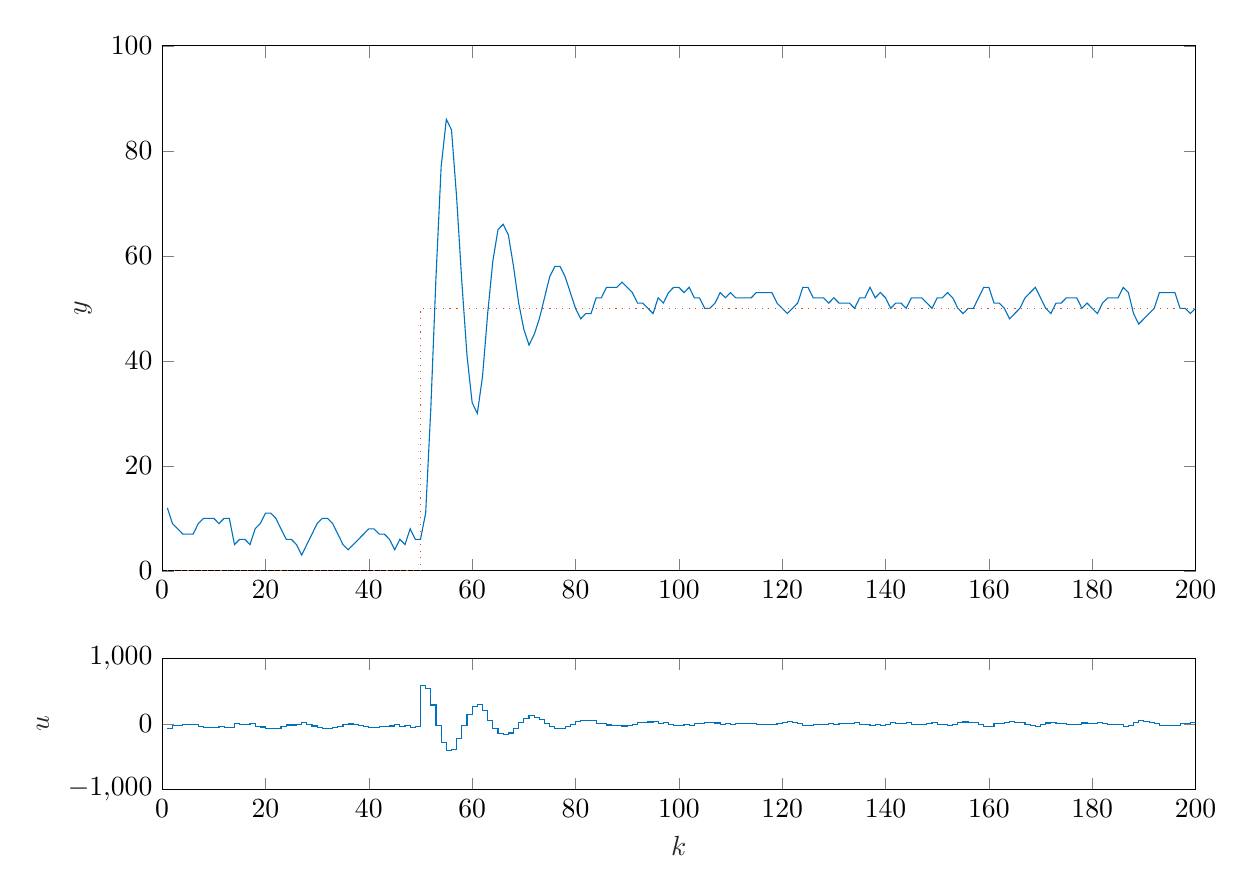
\begin{tikzpicture}

\begin{axis}[%
width=5.167in,
height=0.656in,
at={(0.646in,0.525in)},
scale only axis,
xmin=0,
xmax=200,
xtick={0,20,40,60,80,100,120,140,160,180,200},
xlabel style={font=\color{white!15!black}},
xlabel={$k$},
ymin=-1000,
ymax=1000,
ytick={-1000,0,1000},
ylabel style={font=\color{white!15!black}},
ylabel={$u$},
axis background/.style={fill=white}
]
\addplot[const plot, color=mycolor1, forget plot] table[row sep=crcr] {%
1	-65\\
2	-28.81\\
3	-17.38\\
4	-5.81\\
5	-6.69\\
6	-7.56\\
7	-33.56\\
8	-47.25\\
9	-48.5\\
10	-49.75\\
11	-38.44\\
12	-52.13\\
13	-53.38\\
14	8.19\\
15	-5\\
16	-5.75\\
17	6.06\\
18	-32.25\\
19	-45.81\\
20	-72.06\\
21	-73.44\\
22	-62.25\\
23	-38.38\\
24	-14.25\\
25	-15\\
26	-3.19\\
27	21.31\\
28	-4.19\\
29	-29.94\\
30	-55.94\\
31	-69.63\\
32	-70.88\\
33	-59.56\\
34	-35.56\\
35	-11.31\\
36	0.63\\
37	-12.44\\
38	-25.63\\
39	-38.94\\
40	-52.38\\
41	-53.38\\
42	-41.81\\
43	-42.69\\
44	-31\\
45	-6.63\\
46	-32.25\\
47	-20.44\\
48	-58.75\\
49	-34.63\\
50	592.75\\
51	535.44\\
52	289.06\\
53	-22.63\\
54	-287.19\\
55	-403.63\\
56	-383\\
57	-223.94\\
58	-25.56\\
59	149.69\\
60	263.88\\
61	291.25\\
62	205.81\\
63	56.69\\
64	-68.81\\
65	-145.31\\
66	-159.75\\
67	-136.63\\
68	-63\\
69	23.94\\
70	86.63\\
71	124.81\\
72	100.56\\
73	63.5\\
74	13.5\\
75	-37\\
76	-62.88\\
77	-63.88\\
78	-39.75\\
79	-2.81\\
80	34.5\\
81	59.63\\
82	47.31\\
83	47.44\\
84	9.88\\
85	9.63\\
86	-15.75\\
87	-16.25\\
88	-16.75\\
89	-29.81\\
90	-17.88\\
91	-5.81\\
92	18.94\\
93	18.81\\
94	31.25\\
95	43.81\\
96	6.25\\
97	18.56\\
98	-6.69\\
99	-19.63\\
100	-20.13\\
101	-8.06\\
102	-21\\
103	3.63\\
104	3.38\\
105	28.25\\
106	28.25\\
107	15.69\\
108	-9.56\\
109	2.63\\
110	-10.19\\
111	2\\
112	1.75\\
113	1.5\\
114	1.25\\
115	-11.56\\
116	-11.94\\
117	-12.31\\
118	-12.69\\
119	12.06\\
120	24.5\\
121	37.06\\
122	24.63\\
123	12.06\\
124	-25.75\\
125	-26.25\\
126	-1.63\\
127	-1.88\\
128	-2.13\\
129	10.19\\
130	-2.5\\
131	9.81\\
132	9.69\\
133	9.56\\
134	22\\
135	-3.13\\
136	-3.38\\
137	-28.75\\
138	-4.13\\
139	-16.94\\
140	-4.75\\
141	20.13\\
142	7.56\\
143	7.44\\
144	19.88\\
145	-5.25\\
146	-5.5\\
147	-5.75\\
148	6.56\\
149	19\\
150	-6.13\\
151	-6.38\\
152	-19.19\\
153	-7\\
154	17.88\\
155	30.44\\
156	18\\
157	18\\
158	-7.13\\
159	-32.5\\
160	-33\\
161	4.19\\
162	4.06\\
163	16.5\\
164	41.63\\
165	29.31\\
166	16.88\\
167	-8.25\\
168	-21.06\\
169	-34\\
170	-9.38\\
171	15.5\\
172	28.06\\
173	3.06\\
174	2.94\\
175	-9.75\\
176	-10\\
177	-10.25\\
178	14.63\\
179	2.06\\
180	14.5\\
181	27.06\\
182	2.06\\
183	-10.63\\
184	-10.88\\
185	-11.13\\
186	-36.5\\
187	-24.44\\
188	25.44\\
189	50.69\\
190	38.5\\
191	26.19\\
192	13.75\\
193	-23.94\\
194	-24.31\\
195	-24.69\\
196	-25.06\\
197	12.25\\
198	12.25\\
199	24.81\\
200	12.38\\
};
\end{axis}

\begin{axis}[%
width=5.167in,
height=2.625in,
at={(0.646in,1.619in)},
scale only axis,
xmin=0,
xmax=200,
xtick={0,20,40,60,80,100,120,140,160,180,200},
ymin=0,
ymax=100,
ytick={0,20,40,60,80,100},
ylabel style={font=\color{white!15!black}},
ylabel={$y$},
axis background/.style={fill=white}
]
\addplot [color=mycolor1, forget plot]
  table[row sep=crcr]{%
1	12\\
2	9\\
3	8\\
4	7\\
5	7\\
6	7\\
7	9\\
8	10\\
9	10\\
10	10\\
11	9\\
12	10\\
13	10\\
14	5\\
15	6\\
16	6\\
17	5\\
18	8\\
19	9\\
20	11\\
21	11\\
22	10\\
23	8\\
24	6\\
25	6\\
26	5\\
27	3\\
28	5\\
29	7\\
30	9\\
31	10\\
32	10\\
33	9\\
34	7\\
35	5\\
36	4\\
37	5\\
38	6\\
39	7\\
40	8\\
41	8\\
42	7\\
43	7\\
44	6\\
45	4\\
46	6\\
47	5\\
48	8\\
49	6\\
50	6\\
51	11\\
52	31\\
53	56\\
54	77\\
55	86\\
56	84\\
57	71\\
58	55\\
59	41\\
60	32\\
61	30\\
62	37\\
63	49\\
64	59\\
65	65\\
66	66\\
67	64\\
68	58\\
69	51\\
70	46\\
71	43\\
72	45\\
73	48\\
74	52\\
75	56\\
76	58\\
77	58\\
78	56\\
79	53\\
80	50\\
81	48\\
82	49\\
83	49\\
84	52\\
85	52\\
86	54\\
87	54\\
88	54\\
89	55\\
90	54\\
91	53\\
92	51\\
93	51\\
94	50\\
95	49\\
96	52\\
97	51\\
98	53\\
99	54\\
100	54\\
101	53\\
102	54\\
103	52\\
104	52\\
105	50\\
106	50\\
107	51\\
108	53\\
109	52\\
110	53\\
111	52\\
112	52\\
113	52\\
114	52\\
115	53\\
116	53\\
117	53\\
118	53\\
119	51\\
120	50\\
121	49\\
122	50\\
123	51\\
124	54\\
125	54\\
126	52\\
127	52\\
128	52\\
129	51\\
130	52\\
131	51\\
132	51\\
133	51\\
134	50\\
135	52\\
136	52\\
137	54\\
138	52\\
139	53\\
140	52\\
141	50\\
142	51\\
143	51\\
144	50\\
145	52\\
146	52\\
147	52\\
148	51\\
149	50\\
150	52\\
151	52\\
152	53\\
153	52\\
154	50\\
155	49\\
156	50\\
157	50\\
158	52\\
159	54\\
160	54\\
161	51\\
162	51\\
163	50\\
164	48\\
165	49\\
166	50\\
167	52\\
168	53\\
169	54\\
170	52\\
171	50\\
172	49\\
173	51\\
174	51\\
175	52\\
176	52\\
177	52\\
178	50\\
179	51\\
180	50\\
181	49\\
182	51\\
183	52\\
184	52\\
185	52\\
186	54\\
187	53\\
188	49\\
189	47\\
190	48\\
191	49\\
192	50\\
193	53\\
194	53\\
195	53\\
196	53\\
197	50\\
198	50\\
199	49\\
200	50\\
};
\addplot[const plot, color=mycolor2, dotted, forget plot] table[row sep=crcr] {%
1	0\\
2	0\\
3	0\\
4	0\\
5	0\\
6	0\\
7	0\\
8	0\\
9	0\\
10	0\\
11	0\\
12	0\\
13	0\\
14	0\\
15	0\\
16	0\\
17	0\\
18	0\\
19	0\\
20	0\\
21	0\\
22	0\\
23	0\\
24	0\\
25	0\\
26	0\\
27	0\\
28	0\\
29	0\\
30	0\\
31	0\\
32	0\\
33	0\\
34	0\\
35	0\\
36	0\\
37	0\\
38	0\\
39	0\\
40	0\\
41	0\\
42	0\\
43	0\\
44	0\\
45	0\\
46	0\\
47	0\\
48	0\\
49	0\\
50	50\\
51	50\\
52	50\\
53	50\\
54	50\\
55	50\\
56	50\\
57	50\\
58	50\\
59	50\\
60	50\\
61	50\\
62	50\\
63	50\\
64	50\\
65	50\\
66	50\\
67	50\\
68	50\\
69	50\\
70	50\\
71	50\\
72	50\\
73	50\\
74	50\\
75	50\\
76	50\\
77	50\\
78	50\\
79	50\\
80	50\\
81	50\\
82	50\\
83	50\\
84	50\\
85	50\\
86	50\\
87	50\\
88	50\\
89	50\\
90	50\\
91	50\\
92	50\\
93	50\\
94	50\\
95	50\\
96	50\\
97	50\\
98	50\\
99	50\\
100	50\\
101	50\\
102	50\\
103	50\\
104	50\\
105	50\\
106	50\\
107	50\\
108	50\\
109	50\\
110	50\\
111	50\\
112	50\\
113	50\\
114	50\\
115	50\\
116	50\\
117	50\\
118	50\\
119	50\\
120	50\\
121	50\\
122	50\\
123	50\\
124	50\\
125	50\\
126	50\\
127	50\\
128	50\\
129	50\\
130	50\\
131	50\\
132	50\\
133	50\\
134	50\\
135	50\\
136	50\\
137	50\\
138	50\\
139	50\\
140	50\\
141	50\\
142	50\\
143	50\\
144	50\\
145	50\\
146	50\\
147	50\\
148	50\\
149	50\\
150	50\\
151	50\\
152	50\\
153	50\\
154	50\\
155	50\\
156	50\\
157	50\\
158	50\\
159	50\\
160	50\\
161	50\\
162	50\\
163	50\\
164	50\\
165	50\\
166	50\\
167	50\\
168	50\\
169	50\\
170	50\\
171	50\\
172	50\\
173	50\\
174	50\\
175	50\\
176	50\\
177	50\\
178	50\\
179	50\\
180	50\\
181	50\\
182	50\\
183	50\\
184	50\\
185	50\\
186	50\\
187	50\\
188	50\\
189	50\\
190	50\\
191	50\\
192	50\\
193	50\\
194	50\\
195	50\\
196	50\\
197	50\\
198	50\\
199	50\\
200	50\\
};
\end{axis}
\end{tikzpicture}%
\end{figure}

\begin{figure}[H]
\centering
%err =11764
\definecolor{mycolor1}{rgb}{0.00000,0.44700,0.74100}%
\definecolor{mycolor2}{rgb}{0.85000,0.32500,0.09800}%
%
\begin{tikzpicture}

\begin{axis}[%
width=5.167in,
height=0.656in,
at={(0.646in,0.525in)},
scale only axis,
xmin=0,
xmax=200,
xtick={0,20,40,60,80,100,120,140,160,180,200},
xlabel style={font=\color{white!15!black}},
xlabel={$k$},
ymin=-1000,
ymax=1000,
ytick={-1000,0,1000},
ylabel style={font=\color{white!15!black}},
ylabel={$u$},
axis background/.style={fill=white}
]
\addplot[const plot, color=mycolor1, forget plot] table[row sep=crcr] {%
1	-16.82\\
2	-17.55\\
3	-5.73\\
4	-18.91\\
5	-32.19\\
6	-20.47\\
7	-58.85\\
8	-59.9\\
9	-60.94\\
10	-36.88\\
11	-25.16\\
12	-13.33\\
13	-39.06\\
14	-39.9\\
15	-28.18\\
16	-16.35\\
17	-16.98\\
18	-17.6\\
19	-18.23\\
20	-43.96\\
21	-57.34\\
22	-33.18\\
23	-33.91\\
24	-34.64\\
25	-22.81\\
26	-23.44\\
27	-36.61\\
28	-24.79\\
29	-50.52\\
30	-63.91\\
31	-39.74\\
32	-40.47\\
33	-28.65\\
34	-29.27\\
35	-42.45\\
36	-18.07\\
37	-6.04\\
38	-6.46\\
39	-19.43\\
40	-32.5\\
41	-45.68\\
42	-46.41\\
43	-47.14\\
44	-60.42\\
45	-36.15\\
46	-36.77\\
47	-24.84\\
48	-25.36\\
49	-38.44\\
50	588.54\\
51	517.81\\
52	295.83\\
53	-28.44\\
54	-255\\
55	-383.02\\
56	-361.46\\
57	-226.72\\
58	-28.07\\
59	134.58\\
60	248.39\\
61	250.16\\
62	176.61\\
63	64.79\\
64	-73.07\\
65	-136.77\\
66	-163.33\\
67	-127.34\\
68	-40.83\\
69	33.85\\
70	96.61\\
71	147.34\\
72	98.07\\
73	60.94\\
74	-1.61\\
75	-52.14\\
76	-77.97\\
77	-53.8\\
78	-29.43\\
79	20.26\\
80	32.71\\
81	32.71\\
82	20.16\\
83	20.05\\
84	7.4\\
85	-5.36\\
86	-5.68\\
87	-5.99\\
88	6.25\\
89	6.04\\
90	5.83\\
91	-6.93\\
92	17.86\\
93	5.21\\
94	-7.55\\
95	-7.86\\
96	-8.18\\
97	-8.49\\
98	-8.8\\
99	3.44\\
100	3.23\\
101	28.12\\
102	3.02\\
103	-9.74\\
104	-10.05\\
105	2.19\\
106	14.53\\
107	1.87\\
108	26.77\\
109	14.22\\
110	1.56\\
111	1.35\\
112	-23.96\\
113	-36.93\\
114	-12.34\\
115	-0.1\\
116	12.24\\
117	37.24\\
118	12.24\\
119	-0.42\\
120	-0.63\\
121	11.72\\
122	24.17\\
123	-0.94\\
124	-1.15\\
125	-1.35\\
126	-26.67\\
127	-14.53\\
128	-2.29\\
129	10.05\\
130	9.95\\
131	-2.71\\
132	9.64\\
133	9.53\\
134	-3.13\\
135	9.22\\
136	9.11\\
137	-28.65\\
138	-16.51\\
139	-4.27\\
140	33.18\\
141	20.73\\
142	33.28\\
143	20.83\\
144	-4.27\\
145	-17.03\\
146	-17.34\\
147	-17.66\\
148	-5.42\\
149	-5.63\\
150	-18.39\\
151	6.41\\
152	6.3\\
153	18.75\\
154	18.75\\
155	18.75\\
156	31.3\\
157	6.3\\
158	-18.91\\
159	-6.67\\
160	-6.88\\
161	5.47\\
162	-7.19\\
163	-19.95\\
164	-7.71\\
165	-7.92\\
166	4.43\\
167	16.87\\
168	16.87\\
169	4.32\\
170	4.22\\
171	-8.44\\
172	-21.2\\
173	-21.51\\
174	-9.27\\
175	28.18\\
176	40.83\\
177	41.04\\
178	28.7\\
179	3.7\\
180	-21.51\\
181	-21.82\\
182	-34.69\\
183	-22.55\\
184	-10.31\\
185	27.14\\
186	2.14\\
187	27.14\\
188	14.69\\
189	14.69\\
190	14.69\\
191	2.14\\
192	14.58\\
193	-10.52\\
194	-10.73\\
195	-10.94\\
196	-11.15\\
197	1.2\\
198	1.09\\
199	0.99\\
200	0.89\\
};
\end{axis}

\begin{axis}[%
width=5.167in,
height=2.625in,
at={(0.646in,1.619in)},
scale only axis,
xmin=0,
xmax=200,
xtick={0,20,40,60,80,100,120,140,160,180,200},
ymin=0,
ymax=100,
ytick={0,20,40,60,80,100},
ylabel style={font=\color{white!15!black}},
ylabel={$y$},
axis background/.style={fill=white}
]
\addplot [color=mycolor1, forget plot]
  table[row sep=crcr]{%
1	7\\
2	7\\
3	6\\
4	7\\
5	8\\
6	7\\
7	10\\
8	10\\
9	10\\
10	8\\
11	7\\
12	6\\
13	8\\
14	8\\
15	7\\
16	6\\
17	6\\
18	6\\
19	6\\
20	8\\
21	9\\
22	7\\
23	7\\
24	7\\
25	6\\
26	6\\
27	7\\
28	6\\
29	8\\
30	9\\
31	7\\
32	7\\
33	6\\
34	6\\
35	7\\
36	5\\
37	4\\
38	4\\
39	5\\
40	6\\
41	7\\
42	7\\
43	7\\
44	8\\
45	6\\
46	6\\
47	5\\
48	5\\
49	6\\
50	6\\
51	12\\
52	30\\
53	56\\
54	74\\
55	84\\
56	82\\
57	71\\
58	55\\
59	42\\
60	33\\
61	33\\
62	39\\
63	48\\
64	59\\
65	64\\
66	66\\
67	63\\
68	56\\
69	50\\
70	45\\
71	41\\
72	45\\
73	48\\
74	53\\
75	57\\
76	59\\
77	57\\
78	55\\
79	51\\
80	50\\
81	50\\
82	51\\
83	51\\
84	52\\
85	53\\
86	53\\
87	53\\
88	52\\
89	52\\
90	52\\
91	53\\
92	51\\
93	52\\
94	53\\
95	53\\
96	53\\
97	53\\
98	53\\
99	52\\
100	52\\
101	50\\
102	52\\
103	53\\
104	53\\
105	52\\
106	51\\
107	52\\
108	50\\
109	51\\
110	52\\
111	52\\
112	54\\
113	55\\
114	53\\
115	52\\
116	51\\
117	49\\
118	51\\
119	52\\
120	52\\
121	51\\
122	50\\
123	52\\
124	52\\
125	52\\
126	54\\
127	53\\
128	52\\
129	51\\
130	51\\
131	52\\
132	51\\
133	51\\
134	52\\
135	51\\
136	51\\
137	54\\
138	53\\
139	52\\
140	49\\
141	50\\
142	49\\
143	50\\
144	52\\
145	53\\
146	53\\
147	53\\
148	52\\
149	52\\
150	53\\
151	51\\
152	51\\
153	50\\
154	50\\
155	50\\
156	49\\
157	51\\
158	53\\
159	52\\
160	52\\
161	51\\
162	52\\
163	53\\
164	52\\
165	52\\
166	51\\
167	50\\
168	50\\
169	51\\
170	51\\
171	52\\
172	53\\
173	53\\
174	52\\
175	49\\
176	48\\
177	48\\
178	49\\
179	51\\
180	53\\
181	53\\
182	54\\
183	53\\
184	52\\
185	49\\
186	51\\
187	49\\
188	50\\
189	50\\
190	50\\
191	51\\
192	50\\
193	52\\
194	52\\
195	52\\
196	52\\
197	51\\
198	51\\
199	51\\
200	51\\
};
\addplot[const plot, color=mycolor2, dotted, forget plot] table[row sep=crcr] {%
1	0\\
2	0\\
3	0\\
4	0\\
5	0\\
6	0\\
7	0\\
8	0\\
9	0\\
10	0\\
11	0\\
12	0\\
13	0\\
14	0\\
15	0\\
16	0\\
17	0\\
18	0\\
19	0\\
20	0\\
21	0\\
22	0\\
23	0\\
24	0\\
25	0\\
26	0\\
27	0\\
28	0\\
29	0\\
30	0\\
31	0\\
32	0\\
33	0\\
34	0\\
35	0\\
36	0\\
37	0\\
38	0\\
39	0\\
40	0\\
41	0\\
42	0\\
43	0\\
44	0\\
45	0\\
46	0\\
47	0\\
48	0\\
49	0\\
50	50\\
51	50\\
52	50\\
53	50\\
54	50\\
55	50\\
56	50\\
57	50\\
58	50\\
59	50\\
60	50\\
61	50\\
62	50\\
63	50\\
64	50\\
65	50\\
66	50\\
67	50\\
68	50\\
69	50\\
70	50\\
71	50\\
72	50\\
73	50\\
74	50\\
75	50\\
76	50\\
77	50\\
78	50\\
79	50\\
80	50\\
81	50\\
82	50\\
83	50\\
84	50\\
85	50\\
86	50\\
87	50\\
88	50\\
89	50\\
90	50\\
91	50\\
92	50\\
93	50\\
94	50\\
95	50\\
96	50\\
97	50\\
98	50\\
99	50\\
100	50\\
101	50\\
102	50\\
103	50\\
104	50\\
105	50\\
106	50\\
107	50\\
108	50\\
109	50\\
110	50\\
111	50\\
112	50\\
113	50\\
114	50\\
115	50\\
116	50\\
117	50\\
118	50\\
119	50\\
120	50\\
121	50\\
122	50\\
123	50\\
124	50\\
125	50\\
126	50\\
127	50\\
128	50\\
129	50\\
130	50\\
131	50\\
132	50\\
133	50\\
134	50\\
135	50\\
136	50\\
137	50\\
138	50\\
139	50\\
140	50\\
141	50\\
142	50\\
143	50\\
144	50\\
145	50\\
146	50\\
147	50\\
148	50\\
149	50\\
150	50\\
151	50\\
152	50\\
153	50\\
154	50\\
155	50\\
156	50\\
157	50\\
158	50\\
159	50\\
160	50\\
161	50\\
162	50\\
163	50\\
164	50\\
165	50\\
166	50\\
167	50\\
168	50\\
169	50\\
170	50\\
171	50\\
172	50\\
173	50\\
174	50\\
175	50\\
176	50\\
177	50\\
178	50\\
179	50\\
180	50\\
181	50\\
182	50\\
183	50\\
184	50\\
185	50\\
186	50\\
187	50\\
188	50\\
189	50\\
190	50\\
191	50\\
192	50\\
193	50\\
194	50\\
195	50\\
196	50\\
197	50\\
198	50\\
199	50\\
200	50\\
};
\end{axis}
\end{tikzpicture}%
\end{figure}

\begin{figure}[H]
\centering
%err =64548806
\definecolor{mycolor1}{rgb}{0.00000,0.44700,0.74100}%
\definecolor{mycolor2}{rgb}{0.85000,0.32500,0.09800}%
%
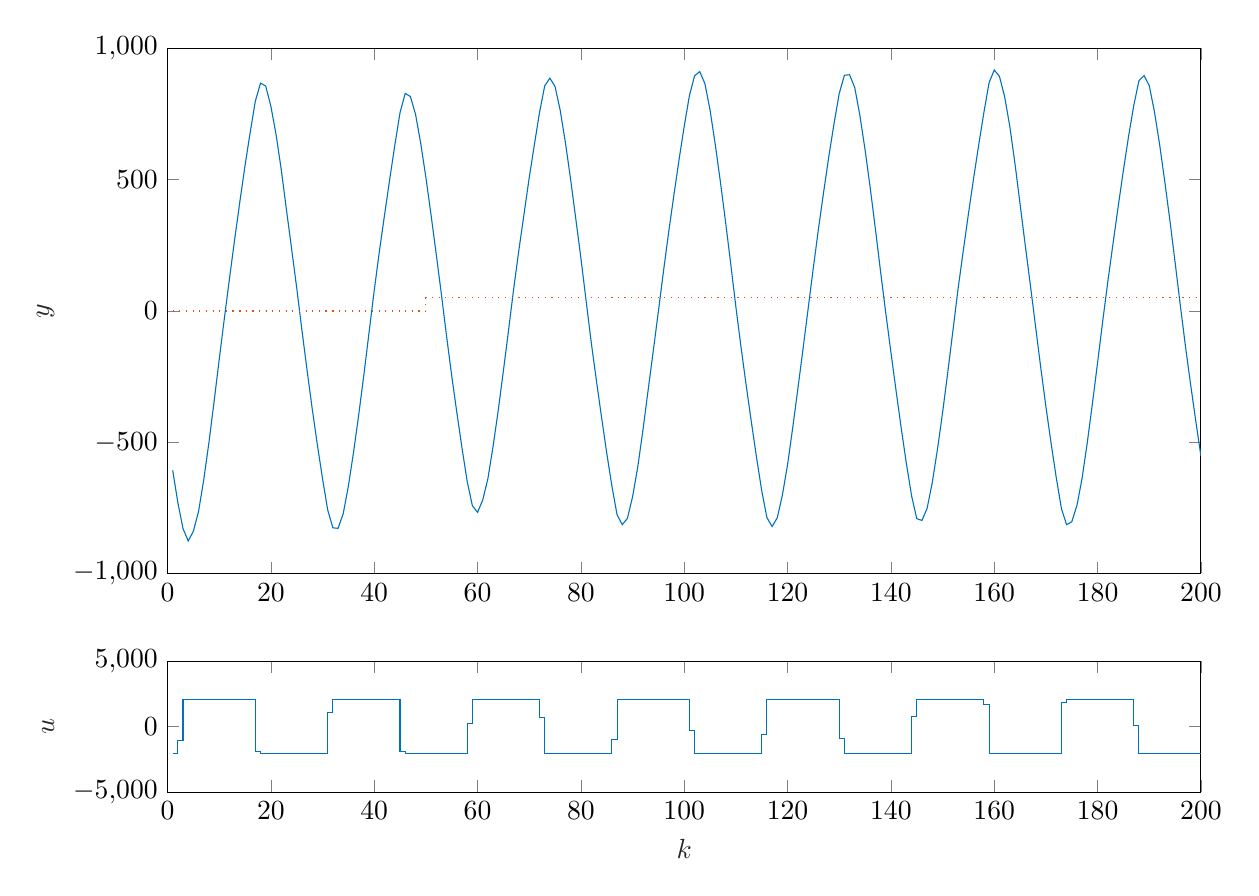
\begin{tikzpicture}

\begin{axis}[%
width=5.167in,
height=0.656in,
at={(0.646in,0.525in)},
scale only axis,
xmin=0,
xmax=200,
xtick={0,20,40,60,80,100,120,140,160,180,200},
xlabel style={font=\color{white!15!black}},
xlabel={$k$},
ymin=-5000,
ymax=5000,
ytick={-5000,0,5000},
ylabel style={font=\color{white!15!black}},
ylabel={$u$},
axis background/.style={fill=white}
]
\addplot[const plot, color=mycolor1, forget plot] table[row sep=crcr] {%
1	-2048\\
2	-1068.75\\
3	2047\\
4	2047\\
5	2047\\
6	2047\\
7	2047\\
8	2047\\
9	2047\\
10	2047\\
11	2047\\
12	2047\\
13	2047\\
14	2047\\
15	2047\\
16	2047\\
17	-1887.5\\
18	-2048\\
19	-2048\\
20	-2048\\
21	-2048\\
22	-2048\\
23	-2048\\
24	-2048\\
25	-2048\\
26	-2048\\
27	-2048\\
28	-2048\\
29	-2048\\
30	-2048\\
31	1106.25\\
32	2047\\
33	2047\\
34	2047\\
35	2047\\
36	2047\\
37	2047\\
38	2047\\
39	2047\\
40	2047\\
41	2047\\
42	2047\\
43	2047\\
44	2047\\
45	-1900\\
46	-2048\\
47	-2048\\
48	-2048\\
49	-2048\\
50	-2048\\
51	-2048\\
52	-2048\\
53	-2048\\
54	-2048\\
55	-2048\\
56	-2048\\
57	-2048\\
58	268.75\\
59	2047\\
60	2047\\
61	2047\\
62	2047\\
63	2047\\
64	2047\\
65	2047\\
66	2047\\
67	2047\\
68	2047\\
69	2047\\
70	2047\\
71	2047\\
72	684.38\\
73	-2048\\
74	-2048\\
75	-2048\\
76	-2048\\
77	-2048\\
78	-2048\\
79	-2048\\
80	-2048\\
81	-2048\\
82	-2048\\
83	-2048\\
84	-2048\\
85	-2048\\
86	-1009.38\\
87	2047\\
88	2047\\
89	2047\\
90	2047\\
91	2047\\
92	2047\\
93	2047\\
94	2047\\
95	2047\\
96	2047\\
97	2047\\
98	2047\\
99	2047\\
100	2047\\
101	-287.5\\
102	-2048\\
103	-2048\\
104	-2048\\
105	-2048\\
106	-2048\\
107	-2048\\
108	-2048\\
109	-2048\\
110	-2048\\
111	-2048\\
112	-2048\\
113	-2048\\
114	-2048\\
115	-596.88\\
116	2047\\
117	2047\\
118	2047\\
119	2047\\
120	2047\\
121	2047\\
122	2047\\
123	2047\\
124	2047\\
125	2047\\
126	2047\\
127	2047\\
128	2047\\
129	2047\\
130	-865.63\\
131	-2048\\
132	-2048\\
133	-2048\\
134	-2048\\
135	-2048\\
136	-2048\\
137	-2048\\
138	-2048\\
139	-2048\\
140	-2048\\
141	-2048\\
142	-2048\\
143	-2048\\
144	781.25\\
145	2047\\
146	2047\\
147	2047\\
148	2047\\
149	2047\\
150	2047\\
151	2047\\
152	2047\\
153	2047\\
154	2047\\
155	2047\\
156	2047\\
157	2047\\
158	1703.13\\
159	-2048\\
160	-2048\\
161	-2048\\
162	-2048\\
163	-2048\\
164	-2048\\
165	-2048\\
166	-2048\\
167	-2048\\
168	-2048\\
169	-2048\\
170	-2048\\
171	-2048\\
172	-2048\\
173	1878.13\\
174	2047\\
175	2047\\
176	2047\\
177	2047\\
178	2047\\
179	2047\\
180	2047\\
181	2047\\
182	2047\\
183	2047\\
184	2047\\
185	2047\\
186	2047\\
187	115.63\\
188	-2048\\
189	-2048\\
190	-2048\\
191	-2048\\
192	-2048\\
193	-2048\\
194	-2048\\
195	-2048\\
196	-2048\\
197	-2048\\
198	-2048\\
199	-2048\\
200	-2048\\
};
\end{axis}

\begin{axis}[%
width=5.167in,
height=2.625in,
at={(0.646in,1.619in)},
scale only axis,
xmin=0,
xmax=200,
xtick={0,20,40,60,80,100,120,140,160,180,200},
ymin=-1000,
ymax=1000,
ytick={-1000,-500,0,500,1000},
ylabel style={font=\color{white!15!black}},
ylabel={$y$},
axis background/.style={fill=white}
]
\addplot [color=mycolor1, forget plot]
  table[row sep=crcr]{%
1	-607\\
2	-730\\
3	-829\\
4	-876\\
5	-839\\
6	-764\\
7	-644\\
8	-503\\
9	-347\\
10	-185\\
11	-28\\
12	125\\
13	274\\
14	417\\
15	554\\
16	681\\
17	800\\
18	868\\
19	857\\
20	780\\
21	673\\
22	540\\
23	388\\
24	239\\
25	88\\
26	-71\\
27	-225\\
28	-372\\
29	-510\\
30	-639\\
31	-758\\
32	-826\\
33	-828\\
34	-772\\
35	-667\\
36	-538\\
37	-396\\
38	-243\\
39	-82\\
40	78\\
41	227\\
42	366\\
43	502\\
44	633\\
45	756\\
46	829\\
47	817\\
48	749\\
49	639\\
50	509\\
51	366\\
52	217\\
53	64\\
54	-95\\
55	-247\\
56	-388\\
57	-523\\
58	-650\\
59	-742\\
60	-767\\
61	-720\\
62	-639\\
63	-516\\
64	-379\\
65	-228\\
66	-73\\
67	86\\
68	232\\
69	370\\
70	508\\
71	634\\
72	757\\
73	858\\
74	887\\
75	855\\
76	764\\
77	642\\
78	503\\
79	353\\
80	202\\
81	40\\
82	-119\\
83	-265\\
84	-405\\
85	-541\\
86	-667\\
87	-776\\
88	-814\\
89	-790\\
90	-708\\
91	-595\\
92	-455\\
93	-303\\
94	-153\\
95	-1\\
96	154\\
97	302\\
98	442\\
99	577\\
100	704\\
101	820\\
102	896\\
103	912\\
104	866\\
105	765\\
106	635\\
107	492\\
108	339\\
109	179\\
110	15\\
111	-139\\
112	-285\\
113	-424\\
114	-559\\
115	-685\\
116	-787\\
117	-821\\
118	-788\\
119	-701\\
120	-585\\
121	-444\\
122	-295\\
123	-143\\
124	12\\
125	167\\
126	316\\
127	456\\
128	591\\
129	715\\
130	829\\
131	898\\
132	900\\
133	851\\
134	744\\
135	614\\
136	468\\
137	312\\
138	150\\
139	-7\\
140	-157\\
141	-304\\
142	-447\\
143	-582\\
144	-704\\
145	-791\\
146	-798\\
147	-752\\
148	-654\\
149	-528\\
150	-387\\
151	-234\\
152	-75\\
153	85\\
154	229\\
155	370\\
156	505\\
157	634\\
158	757\\
159	870\\
160	918\\
161	894\\
162	817\\
163	704\\
164	563\\
165	407\\
166	250\\
167	97\\
168	-60\\
169	-216\\
170	-365\\
171	-504\\
172	-635\\
173	-753\\
174	-814\\
175	-803\\
176	-741\\
177	-637\\
178	-502\\
179	-352\\
180	-196\\
181	-37\\
182	115\\
183	259\\
184	400\\
185	537\\
186	666\\
187	783\\
188	877\\
189	897\\
190	858\\
191	759\\
192	635\\
193	493\\
194	344\\
195	185\\
196	23\\
197	-134\\
198	-280\\
199	-419\\
200	-553\\
};
\addplot[const plot, color=mycolor2, dotted, forget plot] table[row sep=crcr] {%
1	0\\
2	0\\
3	0\\
4	0\\
5	0\\
6	0\\
7	0\\
8	0\\
9	0\\
10	0\\
11	0\\
12	0\\
13	0\\
14	0\\
15	0\\
16	0\\
17	0\\
18	0\\
19	0\\
20	0\\
21	0\\
22	0\\
23	0\\
24	0\\
25	0\\
26	0\\
27	0\\
28	0\\
29	0\\
30	0\\
31	0\\
32	0\\
33	0\\
34	0\\
35	0\\
36	0\\
37	0\\
38	0\\
39	0\\
40	0\\
41	0\\
42	0\\
43	0\\
44	0\\
45	0\\
46	0\\
47	0\\
48	0\\
49	0\\
50	50\\
51	50\\
52	50\\
53	50\\
54	50\\
55	50\\
56	50\\
57	50\\
58	50\\
59	50\\
60	50\\
61	50\\
62	50\\
63	50\\
64	50\\
65	50\\
66	50\\
67	50\\
68	50\\
69	50\\
70	50\\
71	50\\
72	50\\
73	50\\
74	50\\
75	50\\
76	50\\
77	50\\
78	50\\
79	50\\
80	50\\
81	50\\
82	50\\
83	50\\
84	50\\
85	50\\
86	50\\
87	50\\
88	50\\
89	50\\
90	50\\
91	50\\
92	50\\
93	50\\
94	50\\
95	50\\
96	50\\
97	50\\
98	50\\
99	50\\
100	50\\
101	50\\
102	50\\
103	50\\
104	50\\
105	50\\
106	50\\
107	50\\
108	50\\
109	50\\
110	50\\
111	50\\
112	50\\
113	50\\
114	50\\
115	50\\
116	50\\
117	50\\
118	50\\
119	50\\
120	50\\
121	50\\
122	50\\
123	50\\
124	50\\
125	50\\
126	50\\
127	50\\
128	50\\
129	50\\
130	50\\
131	50\\
132	50\\
133	50\\
134	50\\
135	50\\
136	50\\
137	50\\
138	50\\
139	50\\
140	50\\
141	50\\
142	50\\
143	50\\
144	50\\
145	50\\
146	50\\
147	50\\
148	50\\
149	50\\
150	50\\
151	50\\
152	50\\
153	50\\
154	50\\
155	50\\
156	50\\
157	50\\
158	50\\
159	50\\
160	50\\
161	50\\
162	50\\
163	50\\
164	50\\
165	50\\
166	50\\
167	50\\
168	50\\
169	50\\
170	50\\
171	50\\
172	50\\
173	50\\
174	50\\
175	50\\
176	50\\
177	50\\
178	50\\
179	50\\
180	50\\
181	50\\
182	50\\
183	50\\
184	50\\
185	50\\
186	50\\
187	50\\
188	50\\
189	50\\
190	50\\
191	50\\
192	50\\
193	50\\
194	50\\
195	50\\
196	50\\
197	50\\
198	50\\
199	50\\
200	50\\
};
\end{axis}
\end{tikzpicture}%
\end{figure}

\begin{figure}[H]
\centering
%err =52478
\definecolor{mycolor1}{rgb}{0.00000,0.44700,0.74100}%
\definecolor{mycolor2}{rgb}{0.85000,0.32500,0.09800}%
%
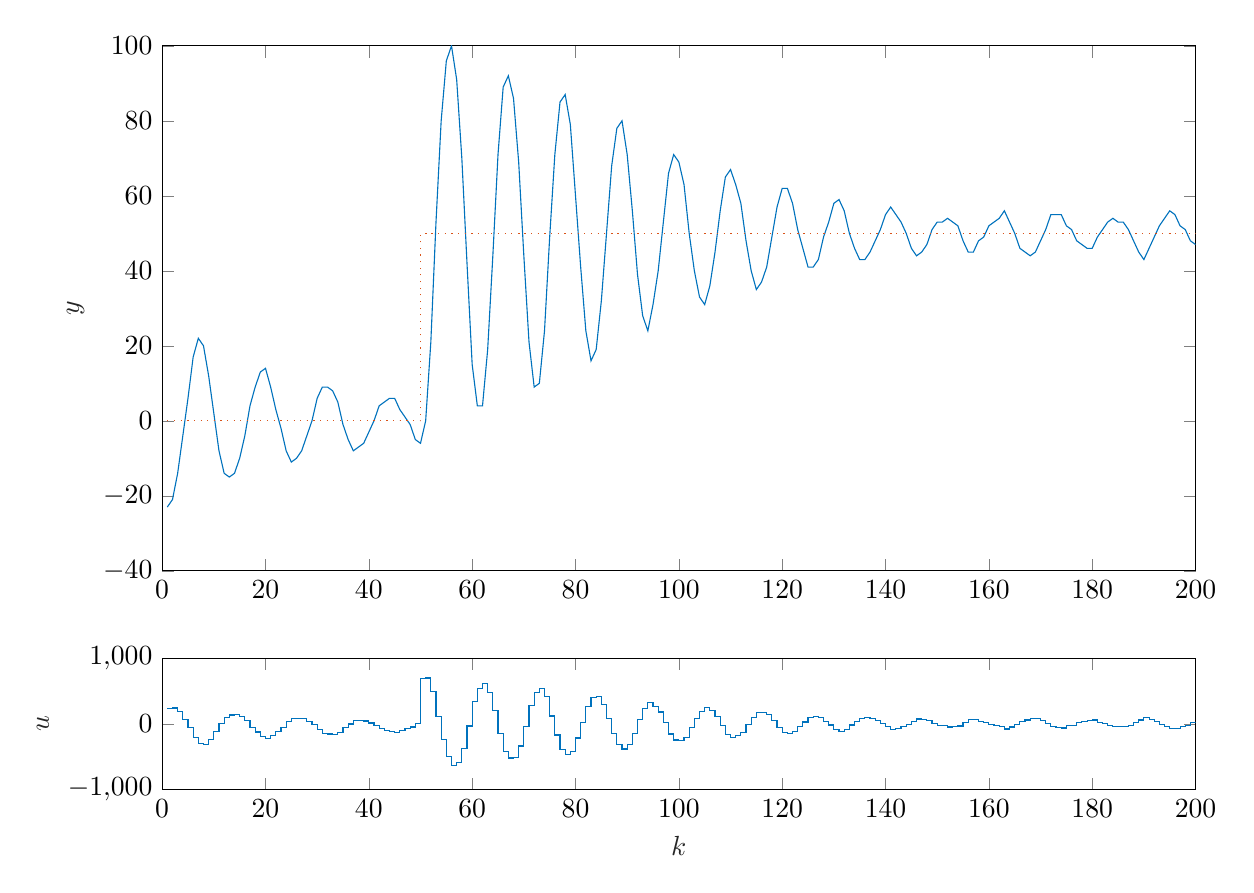
\begin{tikzpicture}

\begin{axis}[%
width=5.167in,
height=0.656in,
at={(0.646in,0.525in)},
scale only axis,
xmin=0,
xmax=200,
xtick={0,20,40,60,80,100,120,140,160,180,200},
xlabel style={font=\color{white!15!black}},
xlabel={$k$},
ymin=-1000,
ymax=1000,
ytick={-1000,0,1000},
ylabel style={font=\color{white!15!black}},
ylabel={$u$},
axis background/.style={fill=white}
]
\addplot[const plot, color=mycolor1, forget plot] table[row sep=crcr] {%
1	235.16\\
2	244.53\\
3	184.38\\
4	73.44\\
5	-53.13\\
6	-208.59\\
7	-301.56\\
8	-309.38\\
9	-234.38\\
10	-120.31\\
11	9.38\\
12	101.56\\
13	136.72\\
14	146.88\\
15	115.63\\
16	51.56\\
17	-48.44\\
18	-121.09\\
19	-188.28\\
20	-221.88\\
21	-177.34\\
22	-111.72\\
23	-50\\
24	32.81\\
25	85.16\\
26	89.06\\
27	78.13\\
28	37.5\\
29	-9.38\\
30	-89.06\\
31	-138.28\\
32	-152.34\\
33	-153.13\\
34	-125.78\\
35	-53.91\\
36	0.78\\
37	48.44\\
38	47.66\\
39	45.31\\
40	14.84\\
41	-20.31\\
42	-73.44\\
43	-92.97\\
44	-114.06\\
45	-123.44\\
46	-92.97\\
47	-71.09\\
48	-46.09\\
49	8.59\\
50	693.75\\
51	701.56\\
52	500.78\\
53	121.09\\
54	-242.19\\
55	-501.56\\
56	-626.56\\
57	-585.16\\
58	-370.31\\
59	-29.69\\
60	341.41\\
61	542.19\\
62	614.06\\
63	486.72\\
64	203.13\\
65	-146.09\\
66	-417.97\\
67	-518.75\\
68	-504.69\\
69	-335.16\\
70	-32.81\\
71	282.03\\
72	486.72\\
73	537.5\\
74	414.06\\
75	122.66\\
76	-167.97\\
77	-386.72\\
78	-467.97\\
79	-419.53\\
80	-212.5\\
81	24.22\\
82	264.06\\
83	410.94\\
84	424.22\\
85	300\\
86	89.06\\
87	-150\\
88	-310.94\\
89	-381.25\\
90	-308.59\\
91	-142.19\\
92	74.22\\
93	237.5\\
94	325\\
95	272.66\\
96	182.81\\
97	25.78\\
98	-151.56\\
99	-242.97\\
100	-249.22\\
101	-199.22\\
102	-46.88\\
103	85.94\\
104	194.53\\
105	247.66\\
106	210.94\\
107	113.28\\
108	-25\\
109	-153.91\\
110	-203.91\\
111	-177.34\\
112	-131.25\\
113	-10.94\\
114	98.44\\
115	180.47\\
116	177.34\\
117	144.53\\
118	52.34\\
119	-52.34\\
120	-129.69\\
121	-148.44\\
122	-114.06\\
123	-33.59\\
124	31.25\\
125	103.91\\
126	117.97\\
127	105.47\\
128	36.72\\
129	-14.84\\
130	-85.94\\
131	-111.72\\
132	-85.94\\
133	-15.63\\
134	37.5\\
135	83.59\\
136	94.53\\
137	78.91\\
138	46.88\\
139	10.16\\
140	-44.53\\
141	-78.91\\
142	-63.28\\
143	-44.53\\
144	-9.38\\
145	43.75\\
146	76.56\\
147	72.66\\
148	53.91\\
149	5.47\\
150	-22.66\\
151	-27.34\\
152	-45.31\\
153	-38.28\\
154	-29.69\\
155	20.31\\
156	63.28\\
157	71.09\\
158	39.06\\
159	28.91\\
160	-9.38\\
161	-25.78\\
162	-43.75\\
163	-76.56\\
164	-46.09\\
165	-10.94\\
166	42.19\\
167	61.72\\
168	82.81\\
169	78.91\\
170	46.88\\
171	10.16\\
172	-44.53\\
173	-52.34\\
174	-60.16\\
175	-28.13\\
176	-17.97\\
177	20.31\\
178	36.72\\
179	54.69\\
180	60.94\\
181	27.34\\
182	2.34\\
183	-25.78\\
184	-43.75\\
185	-36.72\\
186	-41.41\\
187	-19.53\\
188	18.75\\
189	61.72\\
190	96.09\\
191	67.19\\
192	33.59\\
193	-4.69\\
194	-34.38\\
195	-67.19\\
196	-63.28\\
197	-31.25\\
198	-21.09\\
199	17.19\\
200	33.59\\
};
\end{axis}

\begin{axis}[%
width=5.167in,
height=2.625in,
at={(0.646in,1.619in)},
scale only axis,
xmin=0,
xmax=200,
xtick={0,20,40,60,80,100,120,140,160,180,200},
ymin=-40,
ymax=100,
ytick={-40,-20,0,20,40,60,80,100},
ylabel style={font=\color{white!15!black}},
ylabel={$y$},
axis background/.style={fill=white}
]
\addplot [color=mycolor1, forget plot]
  table[row sep=crcr]{%
1	-23\\
2	-21\\
3	-14\\
4	-4\\
5	6\\
6	17\\
7	22\\
8	20\\
9	12\\
10	2\\
11	-8\\
12	-14\\
13	-15\\
14	-14\\
15	-10\\
16	-4\\
17	4\\
18	9\\
19	13\\
20	14\\
21	9\\
22	3\\
23	-2\\
24	-8\\
25	-11\\
26	-10\\
27	-8\\
28	-4\\
29	0\\
30	6\\
31	9\\
32	9\\
33	8\\
34	5\\
35	-1\\
36	-5\\
37	-8\\
38	-7\\
39	-6\\
40	-3\\
41	0\\
42	4\\
43	5\\
44	6\\
45	6\\
46	3\\
47	1\\
48	-1\\
49	-5\\
50	-6\\
51	0\\
52	21\\
53	53\\
54	80\\
55	96\\
56	100\\
57	91\\
58	70\\
59	42\\
60	15\\
61	4\\
62	4\\
63	19\\
64	44\\
65	71\\
66	89\\
67	92\\
68	86\\
69	69\\
70	44\\
71	21\\
72	9\\
73	10\\
74	24\\
75	49\\
76	71\\
77	85\\
78	87\\
79	79\\
80	60\\
81	41\\
82	24\\
83	16\\
84	19\\
85	32\\
86	50\\
87	68\\
88	78\\
89	80\\
90	71\\
91	56\\
92	39\\
93	28\\
94	24\\
95	31\\
96	40\\
97	53\\
98	66\\
99	71\\
100	69\\
101	63\\
102	50\\
103	40\\
104	33\\
105	31\\
106	36\\
107	45\\
108	56\\
109	65\\
110	67\\
111	63\\
112	58\\
113	48\\
114	40\\
115	35\\
116	37\\
117	41\\
118	49\\
119	57\\
120	62\\
121	62\\
122	58\\
123	51\\
124	46\\
125	41\\
126	41\\
127	43\\
128	49\\
129	53\\
130	58\\
131	59\\
132	56\\
133	50\\
134	46\\
135	43\\
136	43\\
137	45\\
138	48\\
139	51\\
140	55\\
141	57\\
142	55\\
143	53\\
144	50\\
145	46\\
146	44\\
147	45\\
148	47\\
149	51\\
150	53\\
151	53\\
152	54\\
153	53\\
154	52\\
155	48\\
156	45\\
157	45\\
158	48\\
159	49\\
160	52\\
161	53\\
162	54\\
163	56\\
164	53\\
165	50\\
166	46\\
167	45\\
168	44\\
169	45\\
170	48\\
171	51\\
172	55\\
173	55\\
174	55\\
175	52\\
176	51\\
177	48\\
178	47\\
179	46\\
180	46\\
181	49\\
182	51\\
183	53\\
184	54\\
185	53\\
186	53\\
187	51\\
188	48\\
189	45\\
190	43\\
191	46\\
192	49\\
193	52\\
194	54\\
195	56\\
196	55\\
197	52\\
198	51\\
199	48\\
200	47\\
};
\addplot[const plot, color=mycolor2, dotted, forget plot] table[row sep=crcr] {%
1	0\\
2	0\\
3	0\\
4	0\\
5	0\\
6	0\\
7	0\\
8	0\\
9	0\\
10	0\\
11	0\\
12	0\\
13	0\\
14	0\\
15	0\\
16	0\\
17	0\\
18	0\\
19	0\\
20	0\\
21	0\\
22	0\\
23	0\\
24	0\\
25	0\\
26	0\\
27	0\\
28	0\\
29	0\\
30	0\\
31	0\\
32	0\\
33	0\\
34	0\\
35	0\\
36	0\\
37	0\\
38	0\\
39	0\\
40	0\\
41	0\\
42	0\\
43	0\\
44	0\\
45	0\\
46	0\\
47	0\\
48	0\\
49	0\\
50	50\\
51	50\\
52	50\\
53	50\\
54	50\\
55	50\\
56	50\\
57	50\\
58	50\\
59	50\\
60	50\\
61	50\\
62	50\\
63	50\\
64	50\\
65	50\\
66	50\\
67	50\\
68	50\\
69	50\\
70	50\\
71	50\\
72	50\\
73	50\\
74	50\\
75	50\\
76	50\\
77	50\\
78	50\\
79	50\\
80	50\\
81	50\\
82	50\\
83	50\\
84	50\\
85	50\\
86	50\\
87	50\\
88	50\\
89	50\\
90	50\\
91	50\\
92	50\\
93	50\\
94	50\\
95	50\\
96	50\\
97	50\\
98	50\\
99	50\\
100	50\\
101	50\\
102	50\\
103	50\\
104	50\\
105	50\\
106	50\\
107	50\\
108	50\\
109	50\\
110	50\\
111	50\\
112	50\\
113	50\\
114	50\\
115	50\\
116	50\\
117	50\\
118	50\\
119	50\\
120	50\\
121	50\\
122	50\\
123	50\\
124	50\\
125	50\\
126	50\\
127	50\\
128	50\\
129	50\\
130	50\\
131	50\\
132	50\\
133	50\\
134	50\\
135	50\\
136	50\\
137	50\\
138	50\\
139	50\\
140	50\\
141	50\\
142	50\\
143	50\\
144	50\\
145	50\\
146	50\\
147	50\\
148	50\\
149	50\\
150	50\\
151	50\\
152	50\\
153	50\\
154	50\\
155	50\\
156	50\\
157	50\\
158	50\\
159	50\\
160	50\\
161	50\\
162	50\\
163	50\\
164	50\\
165	50\\
166	50\\
167	50\\
168	50\\
169	50\\
170	50\\
171	50\\
172	50\\
173	50\\
174	50\\
175	50\\
176	50\\
177	50\\
178	50\\
179	50\\
180	50\\
181	50\\
182	50\\
183	50\\
184	50\\
185	50\\
186	50\\
187	50\\
188	50\\
189	50\\
190	50\\
191	50\\
192	50\\
193	50\\
194	50\\
195	50\\
196	50\\
197	50\\
198	50\\
199	50\\
200	50\\
};
\end{axis}
\end{tikzpicture}%
\end{figure}

\begin{figure}[H]
\centering
%err =13938
\definecolor{mycolor1}{rgb}{0.00000,0.44700,0.74100}%
\definecolor{mycolor2}{rgb}{0.85000,0.32500,0.09800}%
%
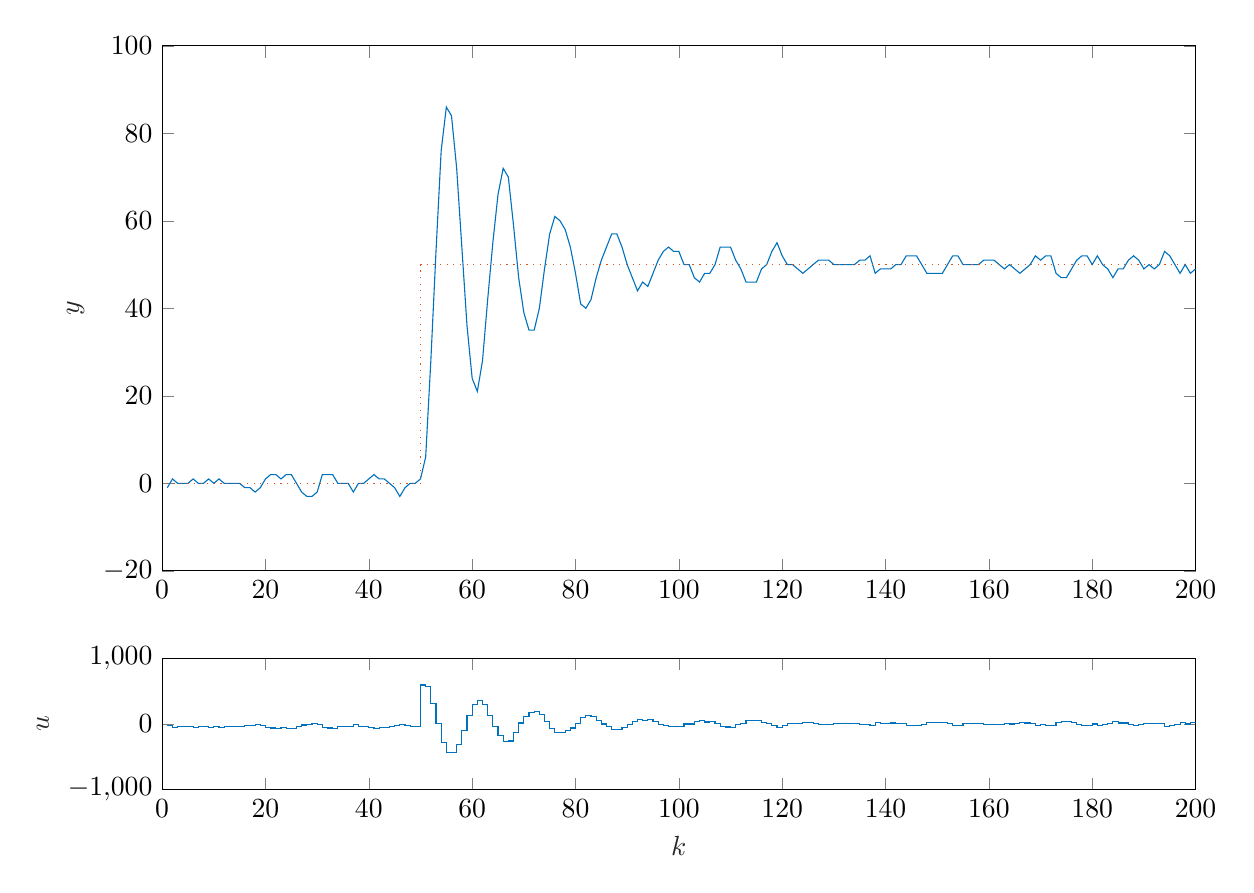
\begin{tikzpicture}

\begin{axis}[%
width=5.167in,
height=0.656in,
at={(0.646in,0.525in)},
scale only axis,
xmin=0,
xmax=200,
xtick={0,20,40,60,80,100,120,140,160,180,200},
xlabel style={font=\color{white!15!black}},
xlabel={$k$},
ymin=-1000,
ymax=1000,
ytick={-1000,0,1000},
ylabel style={font=\color{white!15!black}},
ylabel={$u$},
axis background/.style={fill=white}
]
\addplot[const plot, color=mycolor1, forget plot] table[row sep=crcr] {%
1	-22.27\\
2	-47.27\\
3	-35.16\\
4	-35.16\\
5	-35.16\\
6	-48.05\\
7	-35.94\\
8	-35.94\\
9	-48.83\\
10	-36.72\\
11	-49.61\\
12	-37.5\\
13	-37.5\\
14	-37.5\\
15	-37.5\\
16	-24.61\\
17	-23.83\\
18	-10.16\\
19	-21.48\\
20	-46.48\\
21	-60.16\\
22	-61.72\\
23	-50.39\\
24	-64.06\\
25	-65.63\\
26	-41.41\\
27	-15.63\\
28	-1.17\\
29	1.17\\
30	-9.38\\
31	-59.38\\
32	-60.94\\
33	-62.5\\
34	-38.28\\
35	-38.28\\
36	-38.28\\
37	-12.5\\
38	-36.72\\
39	-36.72\\
40	-49.61\\
41	-63.28\\
42	-51.95\\
43	-52.73\\
44	-40.63\\
45	-27.73\\
46	-1.17\\
47	-24.61\\
48	-36.72\\
49	-36.72\\
50	594.92\\
51	568.75\\
52	319.53\\
53	14.45\\
54	-284.38\\
55	-433.59\\
56	-435.94\\
57	-307.81\\
58	-92.97\\
59	135.94\\
60	301.56\\
61	360.55\\
62	292.97\\
63	129.69\\
64	-31.64\\
65	-177.34\\
66	-267.19\\
67	-258.59\\
68	-132.42\\
69	15.23\\
70	120.7\\
71	180.86\\
72	192.58\\
73	139.84\\
74	31.64\\
75	-70.7\\
76	-127.73\\
77	-123.44\\
78	-105.47\\
79	-60.16\\
80	14.06\\
81	105.86\\
82	125.78\\
83	107.81\\
84	49.61\\
85	0.39\\
86	-39.06\\
87	-80.86\\
88	-86.33\\
89	-53.13\\
90	-4.69\\
91	33.98\\
92	75\\
93	53.91\\
94	69.92\\
95	35.16\\
96	-1.95\\
97	-28.52\\
98	-43.75\\
99	-33.98\\
100	-36.33\\
101	0\\
102	0\\
103	38.67\\
104	53.91\\
105	31.25\\
106	32.81\\
107	8.59\\
108	-42.97\\
109	-46.09\\
110	-49.22\\
111	-13.67\\
112	11.33\\
113	50.78\\
114	53.91\\
115	57.03\\
116	21.48\\
117	9.38\\
118	-29.3\\
119	-57.42\\
120	-22.66\\
121	1.56\\
122	1.56\\
123	14.45\\
124	28.13\\
125	16.8\\
126	4.69\\
127	-8.2\\
128	-8.98\\
129	-9.77\\
130	2.34\\
131	2.34\\
132	2.34\\
133	2.34\\
134	2.34\\
135	-10.55\\
136	-11.33\\
137	-25\\
138	25\\
139	13.67\\
140	14.45\\
141	15.23\\
142	3.13\\
143	3.13\\
144	-22.66\\
145	-24.22\\
146	-25.78\\
147	-1.56\\
148	24.22\\
149	25.78\\
150	27.34\\
151	28.91\\
152	4.69\\
153	-21.09\\
154	-22.66\\
155	1.56\\
156	1.56\\
157	1.56\\
158	1.56\\
159	-11.33\\
160	-12.11\\
161	-12.89\\
162	-0.78\\
163	12.11\\
164	0\\
165	12.89\\
166	26.56\\
167	15.23\\
168	3.13\\
169	-22.66\\
170	-11.33\\
171	-25\\
172	-26.56\\
173	23.44\\
174	37.89\\
175	40.23\\
176	16.8\\
177	-8.2\\
178	-21.88\\
179	-23.44\\
180	0.78\\
181	-25\\
182	-0.78\\
183	12.11\\
184	38.67\\
185	15.23\\
186	16.02\\
187	-8.98\\
188	-22.66\\
189	-11.33\\
190	13.67\\
191	1.56\\
192	14.45\\
193	2.34\\
194	-36.33\\
195	-25.78\\
196	-1.56\\
197	24.22\\
198	0\\
199	25.78\\
200	14.45\\
};
\end{axis}

\begin{axis}[%
width=5.167in,
height=2.625in,
at={(0.646in,1.619in)},
scale only axis,
xmin=0,
xmax=200,
xtick={0,20,40,60,80,100,120,140,160,180,200},
ymin=-20,
ymax=100,
ytick={-20,0,20,40,60,80,100},
ylabel style={font=\color{white!15!black}},
ylabel={$y$},
axis background/.style={fill=white}
]
\addplot [color=mycolor1, forget plot]
  table[row sep=crcr]{%
1	-1\\
2	1\\
3	0\\
4	0\\
5	0\\
6	1\\
7	0\\
8	0\\
9	1\\
10	0\\
11	1\\
12	0\\
13	0\\
14	0\\
15	0\\
16	-1\\
17	-1\\
18	-2\\
19	-1\\
20	1\\
21	2\\
22	2\\
23	1\\
24	2\\
25	2\\
26	0\\
27	-2\\
28	-3\\
29	-3\\
30	-2\\
31	2\\
32	2\\
33	2\\
34	0\\
35	0\\
36	0\\
37	-2\\
38	0\\
39	0\\
40	1\\
41	2\\
42	1\\
43	1\\
44	0\\
45	-1\\
46	-3\\
47	-1\\
48	0\\
49	0\\
50	1\\
51	6\\
52	28\\
53	53\\
54	76\\
55	86\\
56	84\\
57	72\\
58	54\\
59	36\\
60	24\\
61	21\\
62	28\\
63	42\\
64	55\\
65	66\\
66	72\\
67	70\\
68	59\\
69	47\\
70	39\\
71	35\\
72	35\\
73	40\\
74	49\\
75	57\\
76	61\\
77	60\\
78	58\\
79	54\\
80	48\\
81	41\\
82	40\\
83	42\\
84	47\\
85	51\\
86	54\\
87	57\\
88	57\\
89	54\\
90	50\\
91	47\\
92	44\\
93	46\\
94	45\\
95	48\\
96	51\\
97	53\\
98	54\\
99	53\\
100	53\\
101	50\\
102	50\\
103	47\\
104	46\\
105	48\\
106	48\\
107	50\\
108	54\\
109	54\\
110	54\\
111	51\\
112	49\\
113	46\\
114	46\\
115	46\\
116	49\\
117	50\\
118	53\\
119	55\\
120	52\\
121	50\\
122	50\\
123	49\\
124	48\\
125	49\\
126	50\\
127	51\\
128	51\\
129	51\\
130	50\\
131	50\\
132	50\\
133	50\\
134	50\\
135	51\\
136	51\\
137	52\\
138	48\\
139	49\\
140	49\\
141	49\\
142	50\\
143	50\\
144	52\\
145	52\\
146	52\\
147	50\\
148	48\\
149	48\\
150	48\\
151	48\\
152	50\\
153	52\\
154	52\\
155	50\\
156	50\\
157	50\\
158	50\\
159	51\\
160	51\\
161	51\\
162	50\\
163	49\\
164	50\\
165	49\\
166	48\\
167	49\\
168	50\\
169	52\\
170	51\\
171	52\\
172	52\\
173	48\\
174	47\\
175	47\\
176	49\\
177	51\\
178	52\\
179	52\\
180	50\\
181	52\\
182	50\\
183	49\\
184	47\\
185	49\\
186	49\\
187	51\\
188	52\\
189	51\\
190	49\\
191	50\\
192	49\\
193	50\\
194	53\\
195	52\\
196	50\\
197	48\\
198	50\\
199	48\\
200	49\\
};
\addplot[const plot, color=mycolor2, dotted, forget plot] table[row sep=crcr] {%
1	0\\
2	0\\
3	0\\
4	0\\
5	0\\
6	0\\
7	0\\
8	0\\
9	0\\
10	0\\
11	0\\
12	0\\
13	0\\
14	0\\
15	0\\
16	0\\
17	0\\
18	0\\
19	0\\
20	0\\
21	0\\
22	0\\
23	0\\
24	0\\
25	0\\
26	0\\
27	0\\
28	0\\
29	0\\
30	0\\
31	0\\
32	0\\
33	0\\
34	0\\
35	0\\
36	0\\
37	0\\
38	0\\
39	0\\
40	0\\
41	0\\
42	0\\
43	0\\
44	0\\
45	0\\
46	0\\
47	0\\
48	0\\
49	0\\
50	50\\
51	50\\
52	50\\
53	50\\
54	50\\
55	50\\
56	50\\
57	50\\
58	50\\
59	50\\
60	50\\
61	50\\
62	50\\
63	50\\
64	50\\
65	50\\
66	50\\
67	50\\
68	50\\
69	50\\
70	50\\
71	50\\
72	50\\
73	50\\
74	50\\
75	50\\
76	50\\
77	50\\
78	50\\
79	50\\
80	50\\
81	50\\
82	50\\
83	50\\
84	50\\
85	50\\
86	50\\
87	50\\
88	50\\
89	50\\
90	50\\
91	50\\
92	50\\
93	50\\
94	50\\
95	50\\
96	50\\
97	50\\
98	50\\
99	50\\
100	50\\
101	50\\
102	50\\
103	50\\
104	50\\
105	50\\
106	50\\
107	50\\
108	50\\
109	50\\
110	50\\
111	50\\
112	50\\
113	50\\
114	50\\
115	50\\
116	50\\
117	50\\
118	50\\
119	50\\
120	50\\
121	50\\
122	50\\
123	50\\
124	50\\
125	50\\
126	50\\
127	50\\
128	50\\
129	50\\
130	50\\
131	50\\
132	50\\
133	50\\
134	50\\
135	50\\
136	50\\
137	50\\
138	50\\
139	50\\
140	50\\
141	50\\
142	50\\
143	50\\
144	50\\
145	50\\
146	50\\
147	50\\
148	50\\
149	50\\
150	50\\
151	50\\
152	50\\
153	50\\
154	50\\
155	50\\
156	50\\
157	50\\
158	50\\
159	50\\
160	50\\
161	50\\
162	50\\
163	50\\
164	50\\
165	50\\
166	50\\
167	50\\
168	50\\
169	50\\
170	50\\
171	50\\
172	50\\
173	50\\
174	50\\
175	50\\
176	50\\
177	50\\
178	50\\
179	50\\
180	50\\
181	50\\
182	50\\
183	50\\
184	50\\
185	50\\
186	50\\
187	50\\
188	50\\
189	50\\
190	50\\
191	50\\
192	50\\
193	50\\
194	50\\
195	50\\
196	50\\
197	50\\
198	50\\
199	50\\
200	50\\
};
\end{axis}
\end{tikzpicture}%
\end{figure}


\begin{figure}[H]
\centering
%err =6388
\definecolor{mycolor1}{rgb}{0.00000,0.44700,0.74100}%
\definecolor{mycolor2}{rgb}{0.85000,0.32500,0.09800}%
%
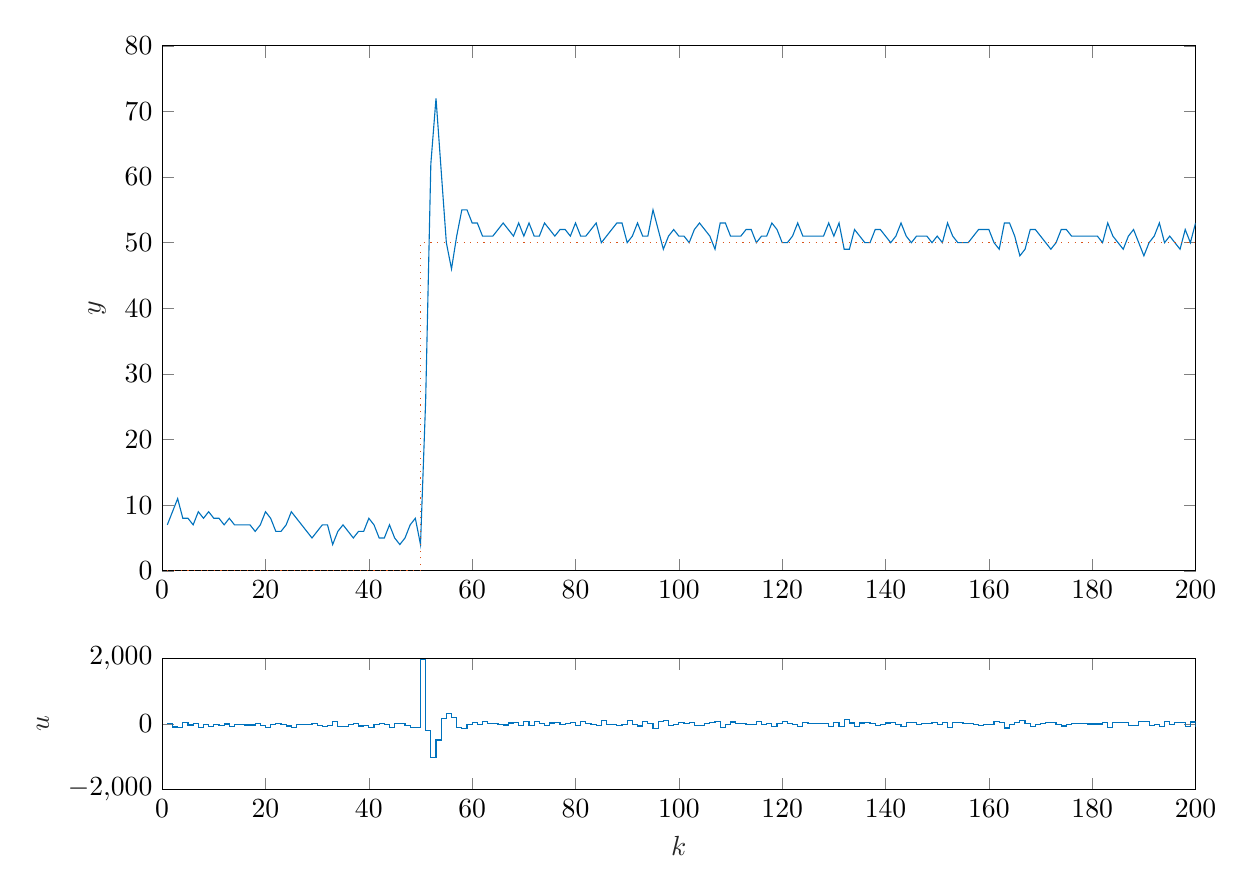
\begin{tikzpicture}

\begin{axis}[%
width=5.167in,
height=0.656in,
at={(0.646in,0.525in)},
scale only axis,
xmin=0,
xmax=200,
xtick={0,20,40,60,80,100,120,140,160,180,200},
xlabel style={font=\color{white!15!black}},
xlabel={$k$},
ymin=-2000,
ymax=2000,
ytick={-2000,0,2000},
ylabel style={font=\color{white!15!black}},
ylabel={$u$},
axis background/.style={fill=white}
]
\addplot[const plot, color=mycolor1, forget plot] table[row sep=crcr] {%
1	10.31\\
2	-90.69\\
3	-116.94\\
4	44.38\\
5	-31.63\\
6	4.94\\
7	-96.06\\
8	-9.63\\
9	-73.19\\
10	-11.75\\
11	-37.75\\
12	-1.19\\
13	-64.63\\
14	-3.06\\
15	-28.94\\
16	-29.81\\
17	-30.69\\
18	6\\
19	-57.31\\
20	-108.31\\
21	-21.88\\
22	27.25\\
23	-23.5\\
24	-61.81\\
25	-112.81\\
26	-26.38\\
27	-14.81\\
28	-3.13\\
29	8.69\\
30	-54.5\\
31	-67.81\\
32	-43.69\\
33	68.13\\
34	-82.5\\
35	-70.81\\
36	-9.13\\
37	2.69\\
38	-60.5\\
39	-36.25\\
40	-112.13\\
41	-25.56\\
42	23.69\\
43	-26.94\\
44	-102.69\\
45	21.56\\
46	8.5\\
47	-54.56\\
48	-105.31\\
49	-93.75\\
50	1958.63\\
51	-212\\
52	-1011.25\\
53	-488.38\\
54	172.06\\
55	308.88\\
56	184.13\\
57	-103.19\\
58	-128.56\\
59	-29.19\\
60	45.31\\
61	-5.06\\
62	69.69\\
63	19.56\\
64	19.44\\
65	-18.25\\
66	-31.06\\
67	31.13\\
68	43.44\\
69	-56.81\\
70	67.94\\
71	-57.31\\
72	67.44\\
73	17.31\\
74	-57.94\\
75	29.25\\
76	41.56\\
77	-21.13\\
78	3.63\\
79	40.94\\
80	-59.31\\
81	65.44\\
82	15.31\\
83	-22.38\\
84	-35.19\\
85	102.13\\
86	-10.44\\
87	-23.13\\
88	-35.94\\
89	-11.31\\
90	101\\
91	-11.56\\
92	-61.81\\
93	62.94\\
94	12.81\\
95	-137.56\\
96	74.5\\
97	111.94\\
98	-38.06\\
99	-25.75\\
100	36.56\\
101	11.44\\
102	48.88\\
103	-51.25\\
104	-39.06\\
105	23.13\\
106	35.44\\
107	85.44\\
108	-114.69\\
109	-15.06\\
110	59.69\\
111	9.56\\
112	9.44\\
113	-28.25\\
114	-3.5\\
115	71.38\\
116	-16.19\\
117	8.69\\
118	-66.56\\
119	20.63\\
120	70.5\\
121	20.5\\
122	-17.06\\
123	-67.31\\
124	57.44\\
125	7.31\\
126	7.19\\
127	7.06\\
128	6.94\\
129	-68.31\\
130	56.44\\
131	-68.81\\
132	131.06\\
133	31.19\\
134	-81.38\\
135	30.94\\
136	43.38\\
137	18.38\\
138	-56.75\\
139	-7\\
140	30.31\\
141	42.75\\
142	-19.81\\
143	-70.06\\
144	54.69\\
145	42.13\\
146	-20.44\\
147	4.44\\
148	4.31\\
149	41.75\\
150	-20.81\\
151	41.63\\
152	-96.06\\
153	53.69\\
154	41.13\\
155	16.13\\
156	16.13\\
157	-21.44\\
158	-34.13\\
159	-9.38\\
160	-9.63\\
161	65.25\\
162	52.81\\
163	-122.31\\
164	-22.69\\
165	52.06\\
166	114.63\\
167	2.31\\
168	-85.25\\
169	-10.5\\
170	26.81\\
171	39.25\\
172	51.81\\
173	-10.63\\
174	-60.75\\
175	-11\\
176	26.31\\
177	1.19\\
178	1.06\\
179	0.94\\
180	0.81\\
181	0.69\\
182	38.13\\
183	-99.56\\
184	50.19\\
185	37.63\\
186	50.19\\
187	-49.81\\
188	-37.5\\
189	62.38\\
190	87.5\\
191	-37.38\\
192	-24.94\\
193	-75.19\\
194	87.13\\
195	-25.44\\
196	37\\
197	49.56\\
198	-88\\
199	61.88\\
200	-100.81\\
};
\end{axis}

\begin{axis}[%
width=5.167in,
height=2.625in,
at={(0.646in,1.619in)},
scale only axis,
xmin=0,
xmax=200,
xtick={0,20,40,60,80,100,120,140,160,180,200},
ymin=0,
ymax=80,
ytick={0,10,20,30,40,50,60,70,80},
ylabel style={font=\color{white!15!black}},
ylabel={$y$},
axis background/.style={fill=white}
]
\addplot [color=mycolor1, forget plot]
  table[row sep=crcr]{%
1	7\\
2	9\\
3	11\\
4	8\\
5	8\\
6	7\\
7	9\\
8	8\\
9	9\\
10	8\\
11	8\\
12	7\\
13	8\\
14	7\\
15	7\\
16	7\\
17	7\\
18	6\\
19	7\\
20	9\\
21	8\\
22	6\\
23	6\\
24	7\\
25	9\\
26	8\\
27	7\\
28	6\\
29	5\\
30	6\\
31	7\\
32	7\\
33	4\\
34	6\\
35	7\\
36	6\\
37	5\\
38	6\\
39	6\\
40	8\\
41	7\\
42	5\\
43	5\\
44	7\\
45	5\\
46	4\\
47	5\\
48	7\\
49	8\\
50	4\\
51	26\\
52	62\\
53	72\\
54	61\\
55	50\\
56	46\\
57	51\\
58	55\\
59	55\\
60	53\\
61	53\\
62	51\\
63	51\\
64	51\\
65	52\\
66	53\\
67	52\\
68	51\\
69	53\\
70	51\\
71	53\\
72	51\\
73	51\\
74	53\\
75	52\\
76	51\\
77	52\\
78	52\\
79	51\\
80	53\\
81	51\\
82	51\\
83	52\\
84	53\\
85	50\\
86	51\\
87	52\\
88	53\\
89	53\\
90	50\\
91	51\\
92	53\\
93	51\\
94	51\\
95	55\\
96	52\\
97	49\\
98	51\\
99	52\\
100	51\\
101	51\\
102	50\\
103	52\\
104	53\\
105	52\\
106	51\\
107	49\\
108	53\\
109	53\\
110	51\\
111	51\\
112	51\\
113	52\\
114	52\\
115	50\\
116	51\\
117	51\\
118	53\\
119	52\\
120	50\\
121	50\\
122	51\\
123	53\\
124	51\\
125	51\\
126	51\\
127	51\\
128	51\\
129	53\\
130	51\\
131	53\\
132	49\\
133	49\\
134	52\\
135	51\\
136	50\\
137	50\\
138	52\\
139	52\\
140	51\\
141	50\\
142	51\\
143	53\\
144	51\\
145	50\\
146	51\\
147	51\\
148	51\\
149	50\\
150	51\\
151	50\\
152	53\\
153	51\\
154	50\\
155	50\\
156	50\\
157	51\\
158	52\\
159	52\\
160	52\\
161	50\\
162	49\\
163	53\\
164	53\\
165	51\\
166	48\\
167	49\\
168	52\\
169	52\\
170	51\\
171	50\\
172	49\\
173	50\\
174	52\\
175	52\\
176	51\\
177	51\\
178	51\\
179	51\\
180	51\\
181	51\\
182	50\\
183	53\\
184	51\\
185	50\\
186	49\\
187	51\\
188	52\\
189	50\\
190	48\\
191	50\\
192	51\\
193	53\\
194	50\\
195	51\\
196	50\\
197	49\\
198	52\\
199	50\\
200	53\\
};
\addplot[const plot, color=mycolor2, dotted, forget plot] table[row sep=crcr] {%
1	0\\
2	0\\
3	0\\
4	0\\
5	0\\
6	0\\
7	0\\
8	0\\
9	0\\
10	0\\
11	0\\
12	0\\
13	0\\
14	0\\
15	0\\
16	0\\
17	0\\
18	0\\
19	0\\
20	0\\
21	0\\
22	0\\
23	0\\
24	0\\
25	0\\
26	0\\
27	0\\
28	0\\
29	0\\
30	0\\
31	0\\
32	0\\
33	0\\
34	0\\
35	0\\
36	0\\
37	0\\
38	0\\
39	0\\
40	0\\
41	0\\
42	0\\
43	0\\
44	0\\
45	0\\
46	0\\
47	0\\
48	0\\
49	0\\
50	50\\
51	50\\
52	50\\
53	50\\
54	50\\
55	50\\
56	50\\
57	50\\
58	50\\
59	50\\
60	50\\
61	50\\
62	50\\
63	50\\
64	50\\
65	50\\
66	50\\
67	50\\
68	50\\
69	50\\
70	50\\
71	50\\
72	50\\
73	50\\
74	50\\
75	50\\
76	50\\
77	50\\
78	50\\
79	50\\
80	50\\
81	50\\
82	50\\
83	50\\
84	50\\
85	50\\
86	50\\
87	50\\
88	50\\
89	50\\
90	50\\
91	50\\
92	50\\
93	50\\
94	50\\
95	50\\
96	50\\
97	50\\
98	50\\
99	50\\
100	50\\
101	50\\
102	50\\
103	50\\
104	50\\
105	50\\
106	50\\
107	50\\
108	50\\
109	50\\
110	50\\
111	50\\
112	50\\
113	50\\
114	50\\
115	50\\
116	50\\
117	50\\
118	50\\
119	50\\
120	50\\
121	50\\
122	50\\
123	50\\
124	50\\
125	50\\
126	50\\
127	50\\
128	50\\
129	50\\
130	50\\
131	50\\
132	50\\
133	50\\
134	50\\
135	50\\
136	50\\
137	50\\
138	50\\
139	50\\
140	50\\
141	50\\
142	50\\
143	50\\
144	50\\
145	50\\
146	50\\
147	50\\
148	50\\
149	50\\
150	50\\
151	50\\
152	50\\
153	50\\
154	50\\
155	50\\
156	50\\
157	50\\
158	50\\
159	50\\
160	50\\
161	50\\
162	50\\
163	50\\
164	50\\
165	50\\
166	50\\
167	50\\
168	50\\
169	50\\
170	50\\
171	50\\
172	50\\
173	50\\
174	50\\
175	50\\
176	50\\
177	50\\
178	50\\
179	50\\
180	50\\
181	50\\
182	50\\
183	50\\
184	50\\
185	50\\
186	50\\
187	50\\
188	50\\
189	50\\
190	50\\
191	50\\
192	50\\
193	50\\
194	50\\
195	50\\
196	50\\
197	50\\
198	50\\
199	50\\
200	50\\
};
\end{axis}
\end{tikzpicture}%
\end{figure}

\begin{figure}[H]
\centering
%err =28562
\definecolor{mycolor1}{rgb}{0.00000,0.44700,0.74100}%
\definecolor{mycolor2}{rgb}{0.85000,0.32500,0.09800}%
%
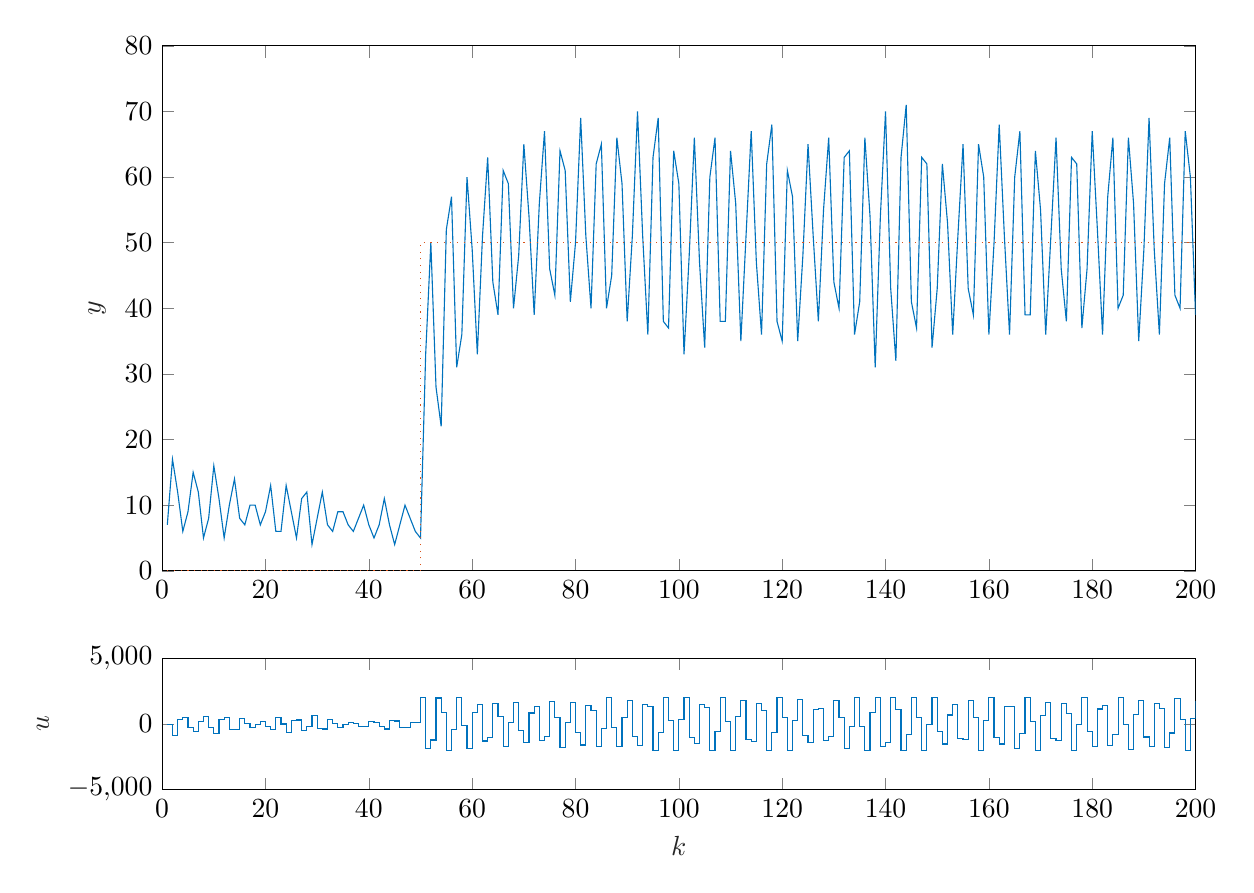
\begin{tikzpicture}

\begin{axis}[%
width=5.167in,
height=0.656in,
at={(0.646in,0.525in)},
scale only axis,
xmin=0,
xmax=200,
xtick={0,20,40,60,80,100,120,140,160,180,200},
xlabel style={font=\color{white!15!black}},
xlabel={$k$},
ymin=-5000,
ymax=5000,
ytick={-5000,0,5000},
ylabel style={font=\color{white!15!black}},
ylabel={$u$},
axis background/.style={fill=white}
]
\addplot[const plot, color=mycolor1, forget plot] table[row sep=crcr] {%
1	-62.69\\
2	-864.19\\
3	321.5\\
4	470.38\\
5	-243.06\\
6	-544.56\\
7	166.25\\
8	552.69\\
9	-235.63\\
10	-712.13\\
11	323.69\\
12	472.69\\
13	-415.75\\
14	-392.25\\
15	431.38\\
16	67.94\\
17	-270.63\\
18	-46.88\\
19	214.56\\
20	-186.44\\
21	-387.81\\
22	523.5\\
23	-2.25\\
24	-615.94\\
25	257.69\\
26	306.81\\
27	-519.19\\
28	-158.13\\
29	615.88\\
30	-334.88\\
31	-386.13\\
32	350.19\\
33	61.87\\
34	-276.56\\
35	-52.69\\
36	121.31\\
37	58\\
38	-192.88\\
39	-219\\
40	192.44\\
41	141.69\\
42	-184.06\\
43	-385.19\\
44	263.69\\
45	225.5\\
46	-262.69\\
47	-301.25\\
48	97.62\\
49	121.75\\
50	2047\\
51	-1834.44\\
52	-1220.88\\
53	1980.5\\
54	858.63\\
55	-2048\\
56	-402.81\\
57	2047\\
58	-137.5\\
59	-1862.25\\
60	899.69\\
61	1475.81\\
62	-1298.19\\
63	-999.06\\
64	1563\\
65	576.56\\
66	-1723.44\\
67	100.31\\
68	1612.88\\
69	-511.38\\
70	-1399.69\\
71	836.63\\
72	1324.56\\
73	-1287.63\\
74	-976.56\\
75	1685.13\\
76	460.87\\
77	-1764.5\\
78	146.44\\
79	1671.31\\
80	-615.63\\
81	-1604.31\\
82	1394.44\\
83	1007.5\\
84	-1742.63\\
85	-356.81\\
86	2047\\
87	-256.19\\
88	-1719.38\\
89	466.56\\
90	1779.25\\
91	-932.56\\
92	-1621.38\\
93	1464.81\\
94	1353.13\\
95	-2048\\
96	-636.31\\
97	2047\\
98	289.81\\
99	-2048\\
100	313.31\\
101	2047\\
102	-1047.5\\
103	-1498.38\\
104	1513.31\\
105	1227\\
106	-2022.63\\
107	-599.25\\
108	2047\\
109	202\\
110	-2048\\
111	575.63\\
112	1813.69\\
113	-1160.44\\
114	-1361.56\\
115	1587.56\\
116	1051.13\\
117	-2048\\
118	-625.63\\
119	2047\\
120	463.19\\
121	-2036.56\\
122	262.31\\
123	1887.81\\
124	-898.63\\
125	-1411.94\\
126	1087.06\\
127	1175.25\\
128	-1286.81\\
129	-975.63\\
130	1773.75\\
131	474.75\\
132	-1837.94\\
133	-202.13\\
134	2047\\
135	-213.19\\
136	-2026.13\\
137	897.63\\
138	2011.06\\
139	-1725.5\\
140	-1402\\
141	2047\\
142	1098.75\\
143	-2048\\
144	-815.56\\
145	2047\\
146	510.06\\
147	-2048\\
148	-29\\
149	2047\\
150	-539.81\\
151	-1527.63\\
152	683.94\\
153	1497.13\\
154	-1089.56\\
155	-1190.56\\
156	1783.94\\
157	485.06\\
158	-2048\\
159	295.75\\
160	2021\\
161	-1003.13\\
162	-1529.25\\
163	1307.06\\
164	1345.38\\
165	-1879.38\\
166	-693.56\\
167	2047\\
168	182.44\\
169	-2005.25\\
170	656.06\\
171	1644.13\\
172	-1092.56\\
173	-1281.13\\
174	1593.13\\
175	794.13\\
176	-1993.44\\
177	-32.5\\
178	2047\\
179	-581.38\\
180	-1744.69\\
181	1141.63\\
182	1417.38\\
183	-1619.69\\
184	-833.63\\
185	2047\\
186	-7.88\\
187	-1958.38\\
188	715.25\\
189	1803.31\\
190	-995.69\\
191	-1696.81\\
192	1552.06\\
193	1190.5\\
194	-1796.69\\
195	-685.75\\
196	1938.75\\
197	314.87\\
198	-2048\\
199	437.75\\
200	1750.31\\
};
\end{axis}

\begin{axis}[%
width=5.167in,
height=2.625in,
at={(0.646in,1.619in)},
scale only axis,
xmin=0,
xmax=200,
xtick={0,20,40,60,80,100,120,140,160,180,200},
ymin=0,
ymax=80,
ytick={0,10,20,30,40,50,60,70,80},
ylabel style={font=\color{white!15!black}},
ylabel={$y$},
axis background/.style={fill=white}
]
\addplot [color=mycolor1, forget plot]
  table[row sep=crcr]{%
1	7\\
2	17\\
3	12\\
4	6\\
5	9\\
6	15\\
7	12\\
8	5\\
9	8\\
10	16\\
11	11\\
12	5\\
13	10\\
14	14\\
15	8\\
16	7\\
17	10\\
18	10\\
19	7\\
20	9\\
21	13\\
22	6\\
23	6\\
24	13\\
25	9\\
26	5\\
27	11\\
28	12\\
29	4\\
30	8\\
31	12\\
32	7\\
33	6\\
34	9\\
35	9\\
36	7\\
37	6\\
38	8\\
39	10\\
40	7\\
41	5\\
42	7\\
43	11\\
44	7\\
45	4\\
46	7\\
47	10\\
48	8\\
49	6\\
50	5\\
51	33\\
52	50\\
53	28\\
54	22\\
55	52\\
56	57\\
57	31\\
58	36\\
59	60\\
60	49\\
61	33\\
62	51\\
63	63\\
64	44\\
65	39\\
66	61\\
67	59\\
68	40\\
69	48\\
70	65\\
71	54\\
72	39\\
73	56\\
74	67\\
75	46\\
76	42\\
77	64\\
78	61\\
79	41\\
80	50\\
81	69\\
82	51\\
83	40\\
84	62\\
85	65\\
86	40\\
87	45\\
88	66\\
89	59\\
90	38\\
91	51\\
92	70\\
93	51\\
94	36\\
95	63\\
96	69\\
97	38\\
98	37\\
99	64\\
100	59\\
101	33\\
102	48\\
103	66\\
104	47\\
105	34\\
106	60\\
107	66\\
108	38\\
109	38\\
110	64\\
111	56\\
112	35\\
113	51\\
114	67\\
115	47\\
116	36\\
117	62\\
118	68\\
119	38\\
120	35\\
121	61\\
122	57\\
123	35\\
124	48\\
125	65\\
126	51\\
127	38\\
128	55\\
129	66\\
130	44\\
131	40\\
132	63\\
133	64\\
134	36\\
135	41\\
136	66\\
137	54\\
138	31\\
139	54\\
140	70\\
141	43\\
142	32\\
143	63\\
144	71\\
145	41\\
146	37\\
147	63\\
148	62\\
149	34\\
150	43\\
151	62\\
152	53\\
153	36\\
154	51\\
155	65\\
156	43\\
157	39\\
158	65\\
159	60\\
160	36\\
161	50\\
162	68\\
163	51\\
164	36\\
165	60\\
166	67\\
167	39\\
168	39\\
169	64\\
170	55\\
171	36\\
172	51\\
173	66\\
174	46\\
175	38\\
176	63\\
177	62\\
178	37\\
179	46\\
180	67\\
181	52\\
182	36\\
183	57\\
184	66\\
185	40\\
186	42\\
187	66\\
188	56\\
189	35\\
190	49\\
191	69\\
192	49\\
193	36\\
194	59\\
195	66\\
196	42\\
197	40\\
198	67\\
199	60\\
200	39\\
};
\addplot[const plot, color=mycolor2, dotted, forget plot] table[row sep=crcr] {%
1	0\\
2	0\\
3	0\\
4	0\\
5	0\\
6	0\\
7	0\\
8	0\\
9	0\\
10	0\\
11	0\\
12	0\\
13	0\\
14	0\\
15	0\\
16	0\\
17	0\\
18	0\\
19	0\\
20	0\\
21	0\\
22	0\\
23	0\\
24	0\\
25	0\\
26	0\\
27	0\\
28	0\\
29	0\\
30	0\\
31	0\\
32	0\\
33	0\\
34	0\\
35	0\\
36	0\\
37	0\\
38	0\\
39	0\\
40	0\\
41	0\\
42	0\\
43	0\\
44	0\\
45	0\\
46	0\\
47	0\\
48	0\\
49	0\\
50	50\\
51	50\\
52	50\\
53	50\\
54	50\\
55	50\\
56	50\\
57	50\\
58	50\\
59	50\\
60	50\\
61	50\\
62	50\\
63	50\\
64	50\\
65	50\\
66	50\\
67	50\\
68	50\\
69	50\\
70	50\\
71	50\\
72	50\\
73	50\\
74	50\\
75	50\\
76	50\\
77	50\\
78	50\\
79	50\\
80	50\\
81	50\\
82	50\\
83	50\\
84	50\\
85	50\\
86	50\\
87	50\\
88	50\\
89	50\\
90	50\\
91	50\\
92	50\\
93	50\\
94	50\\
95	50\\
96	50\\
97	50\\
98	50\\
99	50\\
100	50\\
101	50\\
102	50\\
103	50\\
104	50\\
105	50\\
106	50\\
107	50\\
108	50\\
109	50\\
110	50\\
111	50\\
112	50\\
113	50\\
114	50\\
115	50\\
116	50\\
117	50\\
118	50\\
119	50\\
120	50\\
121	50\\
122	50\\
123	50\\
124	50\\
125	50\\
126	50\\
127	50\\
128	50\\
129	50\\
130	50\\
131	50\\
132	50\\
133	50\\
134	50\\
135	50\\
136	50\\
137	50\\
138	50\\
139	50\\
140	50\\
141	50\\
142	50\\
143	50\\
144	50\\
145	50\\
146	50\\
147	50\\
148	50\\
149	50\\
150	50\\
151	50\\
152	50\\
153	50\\
154	50\\
155	50\\
156	50\\
157	50\\
158	50\\
159	50\\
160	50\\
161	50\\
162	50\\
163	50\\
164	50\\
165	50\\
166	50\\
167	50\\
168	50\\
169	50\\
170	50\\
171	50\\
172	50\\
173	50\\
174	50\\
175	50\\
176	50\\
177	50\\
178	50\\
179	50\\
180	50\\
181	50\\
182	50\\
183	50\\
184	50\\
185	50\\
186	50\\
187	50\\
188	50\\
189	50\\
190	50\\
191	50\\
192	50\\
193	50\\
194	50\\
195	50\\
196	50\\
197	50\\
198	50\\
199	50\\
200	50\\
};
\end{axis}
\end{tikzpicture}%
\end{figure}

\begin{figure}[H]
\centering
%err =4873
\definecolor{mycolor1}{rgb}{0.00000,0.44700,0.74100}%
\definecolor{mycolor2}{rgb}{0.85000,0.32500,0.09800}%
%
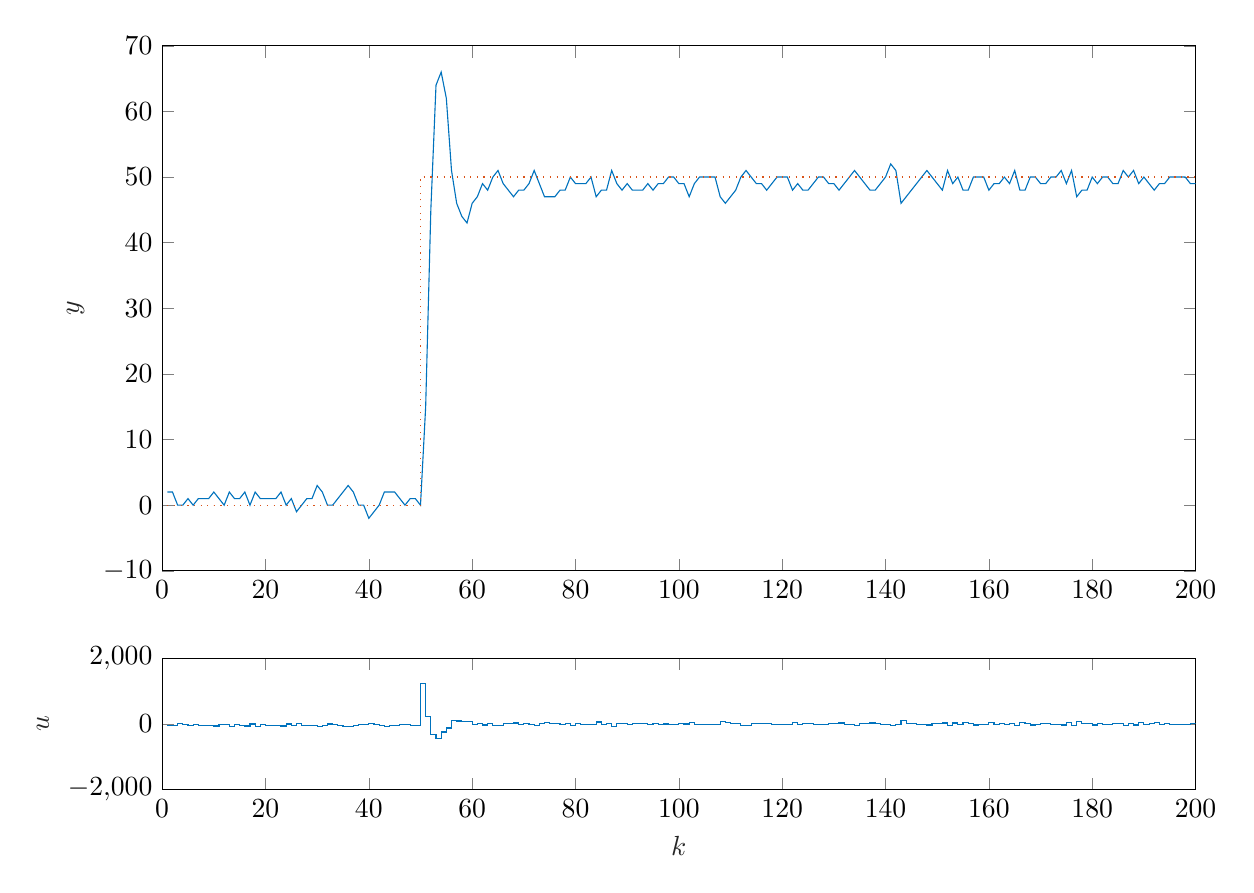
\begin{tikzpicture}

\begin{axis}[%
width=5.167in,
height=0.656in,
at={(0.646in,0.525in)},
scale only axis,
xmin=0,
xmax=200,
xtick={0,20,40,60,80,100,120,140,160,180,200},
xlabel style={font=\color{white!15!black}},
xlabel={$k$},
ymin=-2000,
ymax=2000,
ytick={-2000,0,2000},
ylabel style={font=\color{white!15!black}},
ylabel={$u$},
axis background/.style={fill=white}
]
\addplot[const plot, color=mycolor1, forget plot] table[row sep=crcr] {%
1	-35.25\\
2	-48\\
3	1.87\\
4	-23.13\\
5	-48.19\\
6	-10.75\\
7	-48.31\\
8	-35.94\\
9	-36.06\\
10	-61.25\\
11	-23.94\\
12	-11.5\\
13	-74.13\\
14	-24.31\\
15	-36.94\\
16	-62.13\\
17	0.25\\
18	-74.88\\
19	-25.06\\
20	-37.69\\
21	-37.81\\
22	-37.94\\
23	-63.13\\
24	-0.75\\
25	-50.81\\
26	11.69\\
27	-38.25\\
28	-50.81\\
29	-38.44\\
30	-88.69\\
31	-39\\
32	-1.63\\
33	-26.63\\
34	-51.69\\
35	-64.38\\
36	-77.19\\
37	-40\\
38	-2.63\\
39	-27.63\\
40	22.5\\
41	-27.31\\
42	-39.75\\
43	-77.38\\
44	-52.63\\
45	-52.88\\
46	-28.06\\
47	-15.63\\
48	-53.19\\
49	-40.81\\
50	1237.25\\
51	230.06\\
52	-329.94\\
53	-430.5\\
54	-244.88\\
55	-121.63\\
56	102.56\\
57	90.25\\
58	78.37\\
59	79.19\\
60	-7.63\\
61	5.31\\
62	-31.94\\
63	18.25\\
64	-44.13\\
65	-44.19\\
66	18.31\\
67	18.5\\
68	31.31\\
69	-5.88\\
70	6.87\\
71	-17.94\\
72	-55.44\\
73	19.56\\
74	44.81\\
75	20.19\\
76	20.56\\
77	-4.13\\
78	8.62\\
79	-41.25\\
80	8.81\\
81	-3.56\\
82	-3.44\\
83	-28.38\\
84	59.31\\
85	-2.88\\
86	9.87\\
87	-65.06\\
88	22.44\\
89	22.62\\
90	-14.69\\
91	23\\
92	10.75\\
93	11\\
94	-13.81\\
95	23.87\\
96	-13.44\\
97	-0.81\\
98	-25.75\\
99	-13.25\\
100	11.81\\
101	-0.56\\
102	49.69\\
103	-25.06\\
104	-25\\
105	-12.5\\
106	-12.5\\
107	-12.5\\
108	62.69\\
109	50.62\\
110	13.56\\
111	1.37\\
112	-36\\
113	-36.06\\
114	1.37\\
115	13.94\\
116	1.56\\
117	26.75\\
118	-10.56\\
119	-23\\
120	-10.5\\
121	-10.5\\
122	39.62\\
123	-10.19\\
124	27.5\\
125	15.25\\
126	-9.56\\
127	-22\\
128	-9.5\\
129	15.56\\
130	3.19\\
131	28.37\\
132	-8.94\\
133	-21.38\\
134	-33.94\\
135	3.5\\
136	16.06\\
137	28.75\\
138	16.5\\
139	-8.31\\
140	-20.75\\
141	-58.38\\
142	-8.56\\
143	104.12\\
144	17.06\\
145	4.87\\
146	-7.44\\
147	-19.88\\
148	-32.44\\
149	5\\
150	17.56\\
151	30.25\\
152	-57.19\\
153	30.31\\
154	-19.63\\
155	43\\
156	18.25\\
157	-31.63\\
158	-6.63\\
159	-6.63\\
160	43.5\\
161	-6.31\\
162	6.31\\
163	-18.63\\
164	18.94\\
165	-43.56\\
166	56.5\\
167	19.25\\
168	-30.63\\
169	-5.63\\
170	19.44\\
171	7.06\\
172	-17.88\\
173	-5.38\\
174	-30.44\\
175	32.06\\
176	-42.94\\
177	82.19\\
178	7.5\\
179	20.25\\
180	-29.63\\
181	20.44\\
182	-17\\
183	-4.5\\
184	20.56\\
185	8.19\\
186	-41.81\\
187	8.12\\
188	-29.44\\
189	33.06\\
190	-16.88\\
191	20.69\\
192	33.37\\
193	-3.94\\
194	8.69\\
195	-16.25\\
196	-3.75\\
197	-3.75\\
198	-3.75\\
199	21.31\\
200	8.94\\
};
\end{axis}

\begin{axis}[%
width=5.167in,
height=2.625in,
at={(0.646in,1.619in)},
scale only axis,
xmin=0,
xmax=200,
xtick={0,20,40,60,80,100,120,140,160,180,200},
ymin=-10,
ymax=70,
ytick={-10,0,10,20,30,40,50,60,70},
ylabel style={font=\color{white!15!black}},
ylabel={$y$},
axis background/.style={fill=white}
]
\addplot [color=mycolor1, forget plot]
  table[row sep=crcr]{%
1	2\\
2	2\\
3	0\\
4	0\\
5	1\\
6	0\\
7	1\\
8	1\\
9	1\\
10	2\\
11	1\\
12	0\\
13	2\\
14	1\\
15	1\\
16	2\\
17	0\\
18	2\\
19	1\\
20	1\\
21	1\\
22	1\\
23	2\\
24	0\\
25	1\\
26	-1\\
27	0\\
28	1\\
29	1\\
30	3\\
31	2\\
32	0\\
33	0\\
34	1\\
35	2\\
36	3\\
37	2\\
38	0\\
39	0\\
40	-2\\
41	-1\\
42	0\\
43	2\\
44	2\\
45	2\\
46	1\\
47	0\\
48	1\\
49	1\\
50	0\\
51	15\\
52	45\\
53	64\\
54	66\\
55	62\\
56	51\\
57	46\\
58	44\\
59	43\\
60	46\\
61	47\\
62	49\\
63	48\\
64	50\\
65	51\\
66	49\\
67	48\\
68	47\\
69	48\\
70	48\\
71	49\\
72	51\\
73	49\\
74	47\\
75	47\\
76	47\\
77	48\\
78	48\\
79	50\\
80	49\\
81	49\\
82	49\\
83	50\\
84	47\\
85	48\\
86	48\\
87	51\\
88	49\\
89	48\\
90	49\\
91	48\\
92	48\\
93	48\\
94	49\\
95	48\\
96	49\\
97	49\\
98	50\\
99	50\\
100	49\\
101	49\\
102	47\\
103	49\\
104	50\\
105	50\\
106	50\\
107	50\\
108	47\\
109	46\\
110	47\\
111	48\\
112	50\\
113	51\\
114	50\\
115	49\\
116	49\\
117	48\\
118	49\\
119	50\\
120	50\\
121	50\\
122	48\\
123	49\\
124	48\\
125	48\\
126	49\\
127	50\\
128	50\\
129	49\\
130	49\\
131	48\\
132	49\\
133	50\\
134	51\\
135	50\\
136	49\\
137	48\\
138	48\\
139	49\\
140	50\\
141	52\\
142	51\\
143	46\\
144	47\\
145	48\\
146	49\\
147	50\\
148	51\\
149	50\\
150	49\\
151	48\\
152	51\\
153	49\\
154	50\\
155	48\\
156	48\\
157	50\\
158	50\\
159	50\\
160	48\\
161	49\\
162	49\\
163	50\\
164	49\\
165	51\\
166	48\\
167	48\\
168	50\\
169	50\\
170	49\\
171	49\\
172	50\\
173	50\\
174	51\\
175	49\\
176	51\\
177	47\\
178	48\\
179	48\\
180	50\\
181	49\\
182	50\\
183	50\\
184	49\\
185	49\\
186	51\\
187	50\\
188	51\\
189	49\\
190	50\\
191	49\\
192	48\\
193	49\\
194	49\\
195	50\\
196	50\\
197	50\\
198	50\\
199	49\\
200	49\\
};
\addplot[const plot, color=mycolor2, dotted, forget plot] table[row sep=crcr] {%
1	0\\
2	0\\
3	0\\
4	0\\
5	0\\
6	0\\
7	0\\
8	0\\
9	0\\
10	0\\
11	0\\
12	0\\
13	0\\
14	0\\
15	0\\
16	0\\
17	0\\
18	0\\
19	0\\
20	0\\
21	0\\
22	0\\
23	0\\
24	0\\
25	0\\
26	0\\
27	0\\
28	0\\
29	0\\
30	0\\
31	0\\
32	0\\
33	0\\
34	0\\
35	0\\
36	0\\
37	0\\
38	0\\
39	0\\
40	0\\
41	0\\
42	0\\
43	0\\
44	0\\
45	0\\
46	0\\
47	0\\
48	0\\
49	0\\
50	50\\
51	50\\
52	50\\
53	50\\
54	50\\
55	50\\
56	50\\
57	50\\
58	50\\
59	50\\
60	50\\
61	50\\
62	50\\
63	50\\
64	50\\
65	50\\
66	50\\
67	50\\
68	50\\
69	50\\
70	50\\
71	50\\
72	50\\
73	50\\
74	50\\
75	50\\
76	50\\
77	50\\
78	50\\
79	50\\
80	50\\
81	50\\
82	50\\
83	50\\
84	50\\
85	50\\
86	50\\
87	50\\
88	50\\
89	50\\
90	50\\
91	50\\
92	50\\
93	50\\
94	50\\
95	50\\
96	50\\
97	50\\
98	50\\
99	50\\
100	50\\
101	50\\
102	50\\
103	50\\
104	50\\
105	50\\
106	50\\
107	50\\
108	50\\
109	50\\
110	50\\
111	50\\
112	50\\
113	50\\
114	50\\
115	50\\
116	50\\
117	50\\
118	50\\
119	50\\
120	50\\
121	50\\
122	50\\
123	50\\
124	50\\
125	50\\
126	50\\
127	50\\
128	50\\
129	50\\
130	50\\
131	50\\
132	50\\
133	50\\
134	50\\
135	50\\
136	50\\
137	50\\
138	50\\
139	50\\
140	50\\
141	50\\
142	50\\
143	50\\
144	50\\
145	50\\
146	50\\
147	50\\
148	50\\
149	50\\
150	50\\
151	50\\
152	50\\
153	50\\
154	50\\
155	50\\
156	50\\
157	50\\
158	50\\
159	50\\
160	50\\
161	50\\
162	50\\
163	50\\
164	50\\
165	50\\
166	50\\
167	50\\
168	50\\
169	50\\
170	50\\
171	50\\
172	50\\
173	50\\
174	50\\
175	50\\
176	50\\
177	50\\
178	50\\
179	50\\
180	50\\
181	50\\
182	50\\
183	50\\
184	50\\
185	50\\
186	50\\
187	50\\
188	50\\
189	50\\
190	50\\
191	50\\
192	50\\
193	50\\
194	50\\
195	50\\
196	50\\
197	50\\
198	50\\
199	50\\
200	50\\
};
\end{axis}
\end{tikzpicture}%
\end{figure}


\begin{figure}[H]
\centering
%err =8032
\definecolor{mycolor1}{rgb}{0.00000,0.44700,0.74100}%
\definecolor{mycolor2}{rgb}{0.85000,0.32500,0.09800}%
%
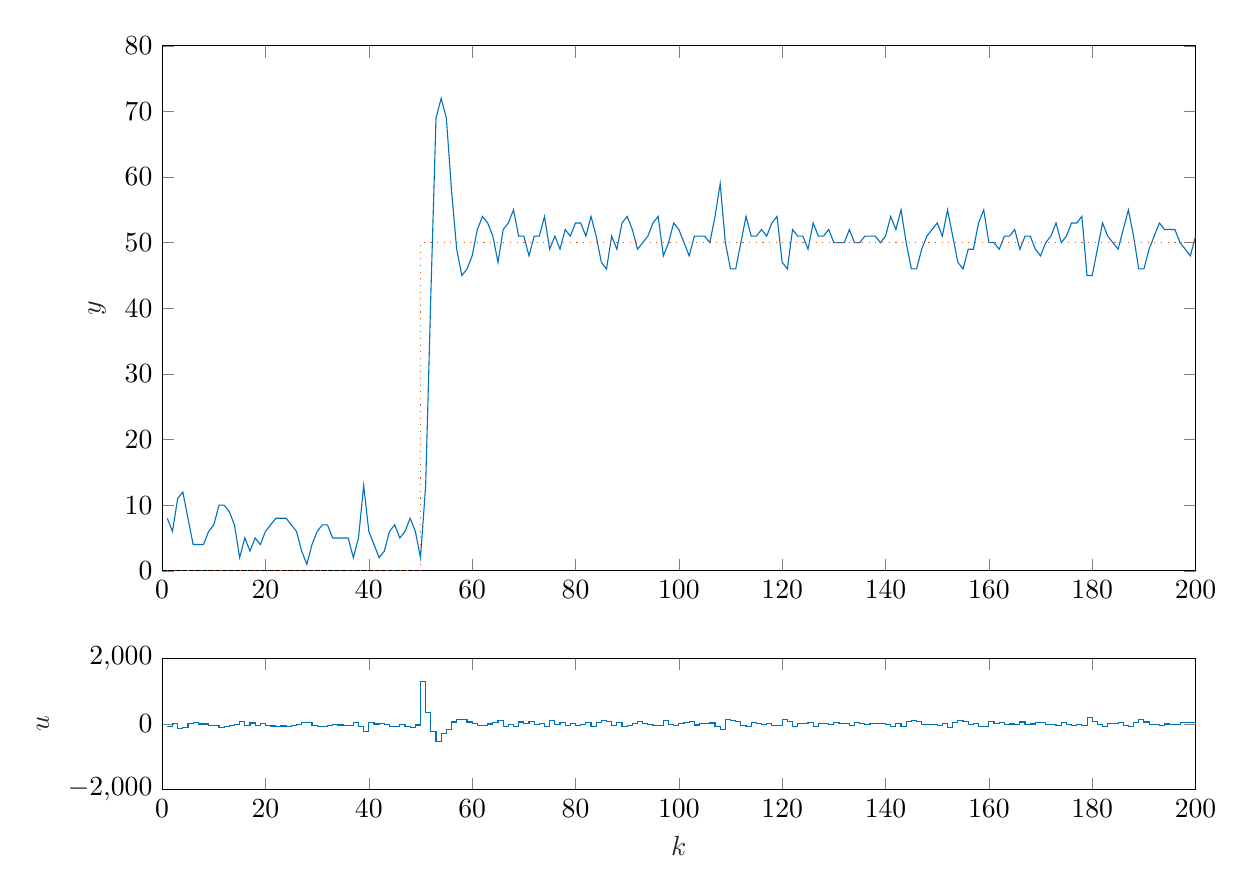
\begin{tikzpicture}

\begin{axis}[%
width=5.167in,
height=0.656in,
at={(0.646in,0.525in)},
scale only axis,
xmin=0,
xmax=200,
xtick={0,20,40,60,80,100,120,140,160,180,200},
xlabel style={font=\color{white!15!black}},
xlabel={$k$},
ymin=-2000,
ymax=2000,
ytick={-2000,0,2000},
ylabel style={font=\color{white!15!black}},
ylabel={$u$},
axis background/.style={fill=white}
]
\addplot[const plot, color=mycolor1, forget plot] table[row sep=crcr] {%
1	-81.6\\
2	5.02\\
3	-146.04\\
4	-109.98\\
5	1.27\\
6	50.52\\
7	0.02\\
8	-0.48\\
9	-51.1\\
10	-51.91\\
11	-115.48\\
12	-79.23\\
13	-55.41\\
14	-18.91\\
15	80.52\\
16	-57.41\\
17	29.59\\
18	-45.91\\
19	3.52\\
20	-59.6\\
21	-60.41\\
22	-73.85\\
23	-62.35\\
24	-63.35\\
25	-39.29\\
26	-27.6\\
27	34.34\\
28	46.59\\
29	-53.73\\
30	-66.85\\
31	-67.66\\
32	-56.04\\
33	-6.79\\
34	-32.41\\
35	-33.04\\
36	-33.66\\
37	40.9\\
38	-72.04\\
39	-235.66\\
40	38.15\\
41	0.02\\
42	24.65\\
43	-25.66\\
44	-88.73\\
45	-77.04\\
46	-15.29\\
47	-65.98\\
48	-104.35\\
49	-30.23\\
50	1297.4\\
51	352.71\\
52	-231.98\\
53	-545.16\\
54	-285.23\\
55	-175.29\\
56	60.52\\
57	147.59\\
58	135.46\\
59	61.02\\
60	23.9\\
61	-51.1\\
62	-51.48\\
63	-1.91\\
64	35.34\\
65	110.46\\
66	-64.48\\
67	-27.29\\
68	-65.29\\
69	59.34\\
70	9.21\\
71	84.27\\
72	-28.16\\
73	9.21\\
74	-66.1\\
75	96.21\\
76	-16.29\\
77	58.71\\
78	-41.35\\
79	20.96\\
80	-41.79\\
81	-17.16\\
82	32.59\\
83	-67.73\\
84	44.46\\
85	107.09\\
86	82.52\\
87	-54.79\\
88	57.71\\
89	-67.41\\
90	-42.85\\
91	19.27\\
92	69.21\\
93	6.77\\
94	-5.79\\
95	-43.54\\
96	-43.98\\
97	118.4\\
98	-6.48\\
99	-56.66\\
100	5.52\\
101	42.9\\
102	68.02\\
103	-31.91\\
104	5.46\\
105	5.34\\
106	30.27\\
107	-82.48\\
108	-158.29\\
109	128.65\\
110	116.4\\
111	66.9\\
112	-32.85\\
113	-83.1\\
114	41.59\\
115	3.96\\
116	-21.23\\
117	16.09\\
118	-46.66\\
119	-47.1\\
120	140.34\\
121	78.27\\
122	-84.1\\
123	15.71\\
124	3.09\\
125	53.09\\
126	-72.04\\
127	27.71\\
128	2.59\\
129	-22.6\\
130	39.77\\
131	14.77\\
132	14.77\\
133	-35.35\\
134	39.52\\
135	14.52\\
136	-10.54\\
137	1.84\\
138	1.71\\
139	26.65\\
140	-10.91\\
141	-73.73\\
142	13.4\\
143	-87.04\\
144	75.15\\
145	112.9\\
146	63.4\\
147	-11.29\\
148	-23.79\\
149	-23.98\\
150	-36.79\\
151	25.46\\
152	-99.91\\
153	49.71\\
154	99.84\\
155	75.27\\
156	-11.91\\
157	25.71\\
158	-74.41\\
159	-74.91\\
160	74.77\\
161	12.27\\
162	37.34\\
163	-25.16\\
164	-0.29\\
165	-25.48\\
166	61.96\\
167	-25.54\\
168	-0.66\\
169	49.34\\
170	49.52\\
171	-12.85\\
172	-12.91\\
173	-50.66\\
174	49.15\\
175	-13.41\\
176	-51.16\\
177	-26.54\\
178	-51.98\\
179	185.59\\
180	73.71\\
181	-25.91\\
182	-76.04\\
183	23.71\\
184	23.65\\
185	36.21\\
186	-51.35\\
187	-89.29\\
188	47.84\\
189	123.02\\
190	61.02\\
191	-13.66\\
192	-26.16\\
193	-51.41\\
194	-1.73\\
195	-14.48\\
196	-14.73\\
197	35.15\\
198	35.21\\
199	47.9\\
200	-39.54\\
};
\end{axis}

\begin{axis}[%
width=5.167in,
height=2.625in,
at={(0.646in,1.619in)},
scale only axis,
xmin=0,
xmax=200,
xtick={0,20,40,60,80,100,120,140,160,180,200},
ymin=0,
ymax=80,
ytick={0,10,20,30,40,50,60,70,80},
ylabel style={font=\color{white!15!black}},
ylabel={$y$},
axis background/.style={fill=white}
]
\addplot [color=mycolor1, forget plot]
  table[row sep=crcr]{%
1	8\\
2	6\\
3	11\\
4	12\\
5	8\\
6	4\\
7	4\\
8	4\\
9	6\\
10	7\\
11	10\\
12	10\\
13	9\\
14	7\\
15	2\\
16	5\\
17	3\\
18	5\\
19	4\\
20	6\\
21	7\\
22	8\\
23	8\\
24	8\\
25	7\\
26	6\\
27	3\\
28	1\\
29	4\\
30	6\\
31	7\\
32	7\\
33	5\\
34	5\\
35	5\\
36	5\\
37	2\\
38	5\\
39	13\\
40	6\\
41	4\\
42	2\\
43	3\\
44	6\\
45	7\\
46	5\\
47	6\\
48	8\\
49	6\\
50	2\\
51	13\\
52	42\\
53	69\\
54	72\\
55	69\\
56	58\\
57	49\\
58	45\\
59	46\\
60	48\\
61	52\\
62	54\\
63	53\\
64	51\\
65	47\\
66	52\\
67	53\\
68	55\\
69	51\\
70	51\\
71	48\\
72	51\\
73	51\\
74	54\\
75	49\\
76	51\\
77	49\\
78	52\\
79	51\\
80	53\\
81	53\\
82	51\\
83	54\\
84	51\\
85	47\\
86	46\\
87	51\\
88	49\\
89	53\\
90	54\\
91	52\\
92	49\\
93	50\\
94	51\\
95	53\\
96	54\\
97	48\\
98	50\\
99	53\\
100	52\\
101	50\\
102	48\\
103	51\\
104	51\\
105	51\\
106	50\\
107	54\\
108	59\\
109	50\\
110	46\\
111	46\\
112	50\\
113	54\\
114	51\\
115	51\\
116	52\\
117	51\\
118	53\\
119	54\\
120	47\\
121	46\\
122	52\\
123	51\\
124	51\\
125	49\\
126	53\\
127	51\\
128	51\\
129	52\\
130	50\\
131	50\\
132	50\\
133	52\\
134	50\\
135	50\\
136	51\\
137	51\\
138	51\\
139	50\\
140	51\\
141	54\\
142	52\\
143	55\\
144	50\\
145	46\\
146	46\\
147	49\\
148	51\\
149	52\\
150	53\\
151	51\\
152	55\\
153	51\\
154	47\\
155	46\\
156	49\\
157	49\\
158	53\\
159	55\\
160	50\\
161	50\\
162	49\\
163	51\\
164	51\\
165	52\\
166	49\\
167	51\\
168	51\\
169	49\\
170	48\\
171	50\\
172	51\\
173	53\\
174	50\\
175	51\\
176	53\\
177	53\\
178	54\\
179	45\\
180	45\\
181	49\\
182	53\\
183	51\\
184	50\\
185	49\\
186	52\\
187	55\\
188	51\\
189	46\\
190	46\\
191	49\\
192	51\\
193	53\\
194	52\\
195	52\\
196	52\\
197	50\\
198	49\\
199	48\\
200	51\\
};
\addplot[const plot, color=mycolor2, dotted, forget plot] table[row sep=crcr] {%
1	0\\
2	0\\
3	0\\
4	0\\
5	0\\
6	0\\
7	0\\
8	0\\
9	0\\
10	0\\
11	0\\
12	0\\
13	0\\
14	0\\
15	0\\
16	0\\
17	0\\
18	0\\
19	0\\
20	0\\
21	0\\
22	0\\
23	0\\
24	0\\
25	0\\
26	0\\
27	0\\
28	0\\
29	0\\
30	0\\
31	0\\
32	0\\
33	0\\
34	0\\
35	0\\
36	0\\
37	0\\
38	0\\
39	0\\
40	0\\
41	0\\
42	0\\
43	0\\
44	0\\
45	0\\
46	0\\
47	0\\
48	0\\
49	0\\
50	50\\
51	50\\
52	50\\
53	50\\
54	50\\
55	50\\
56	50\\
57	50\\
58	50\\
59	50\\
60	50\\
61	50\\
62	50\\
63	50\\
64	50\\
65	50\\
66	50\\
67	50\\
68	50\\
69	50\\
70	50\\
71	50\\
72	50\\
73	50\\
74	50\\
75	50\\
76	50\\
77	50\\
78	50\\
79	50\\
80	50\\
81	50\\
82	50\\
83	50\\
84	50\\
85	50\\
86	50\\
87	50\\
88	50\\
89	50\\
90	50\\
91	50\\
92	50\\
93	50\\
94	50\\
95	50\\
96	50\\
97	50\\
98	50\\
99	50\\
100	50\\
101	50\\
102	50\\
103	50\\
104	50\\
105	50\\
106	50\\
107	50\\
108	50\\
109	50\\
110	50\\
111	50\\
112	50\\
113	50\\
114	50\\
115	50\\
116	50\\
117	50\\
118	50\\
119	50\\
120	50\\
121	50\\
122	50\\
123	50\\
124	50\\
125	50\\
126	50\\
127	50\\
128	50\\
129	50\\
130	50\\
131	50\\
132	50\\
133	50\\
134	50\\
135	50\\
136	50\\
137	50\\
138	50\\
139	50\\
140	50\\
141	50\\
142	50\\
143	50\\
144	50\\
145	50\\
146	50\\
147	50\\
148	50\\
149	50\\
150	50\\
151	50\\
152	50\\
153	50\\
154	50\\
155	50\\
156	50\\
157	50\\
158	50\\
159	50\\
160	50\\
161	50\\
162	50\\
163	50\\
164	50\\
165	50\\
166	50\\
167	50\\
168	50\\
169	50\\
170	50\\
171	50\\
172	50\\
173	50\\
174	50\\
175	50\\
176	50\\
177	50\\
178	50\\
179	50\\
180	50\\
181	50\\
182	50\\
183	50\\
184	50\\
185	50\\
186	50\\
187	50\\
188	50\\
189	50\\
190	50\\
191	50\\
192	50\\
193	50\\
194	50\\
195	50\\
196	50\\
197	50\\
198	50\\
199	50\\
200	50\\
};
\end{axis}
\end{tikzpicture}%
\end{figure}

\begin{figure}[H]
\centering
%err =5114
\definecolor{mycolor1}{rgb}{0.00000,0.44700,0.74100}%
\definecolor{mycolor2}{rgb}{0.85000,0.32500,0.09800}%
%
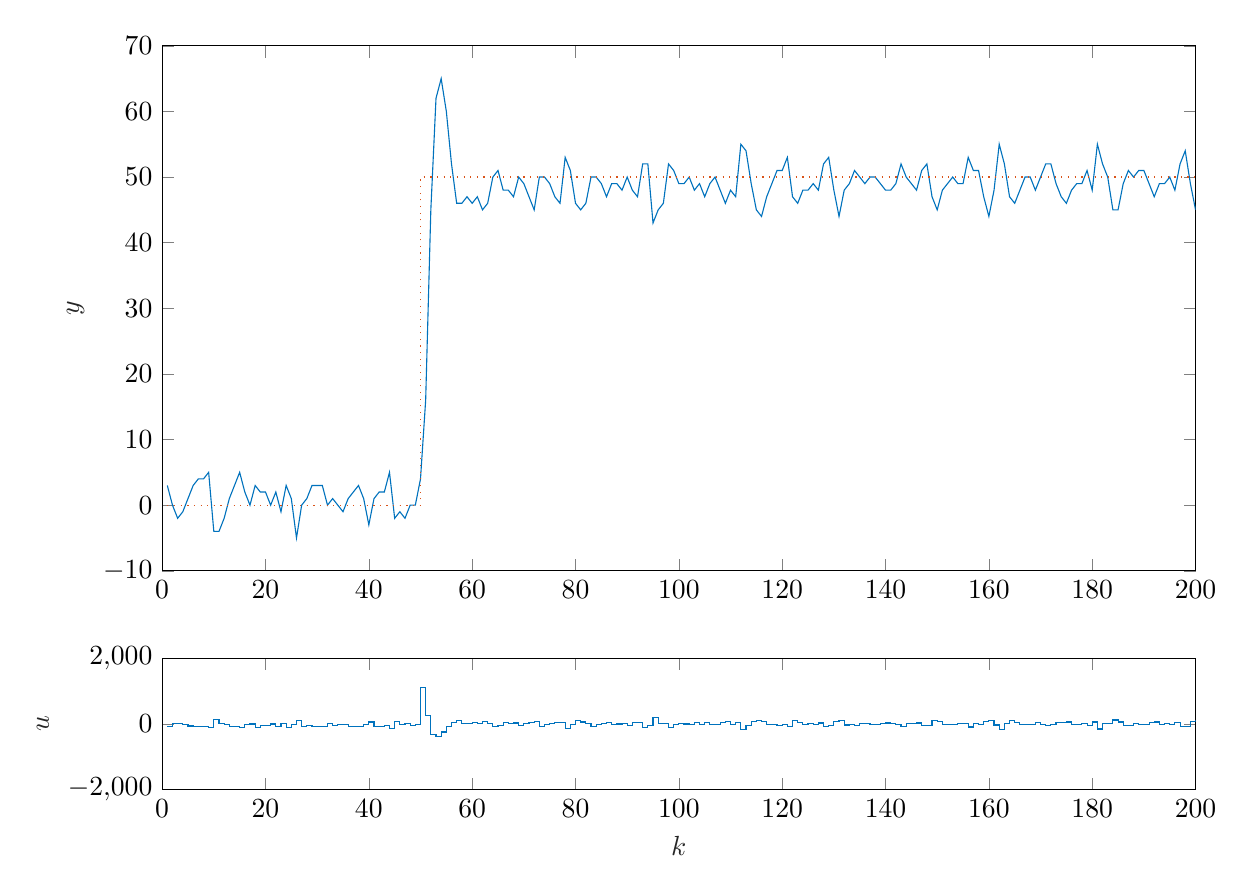
\begin{tikzpicture}

\begin{axis}[%
width=5.167in,
height=0.656in,
at={(0.646in,0.525in)},
scale only axis,
xmin=0,
xmax=200,
xtick={0,20,40,60,80,100,120,140,160,180,200},
xlabel style={font=\color{white!15!black}},
xlabel={$k$},
ymin=-2000,
ymax=2000,
ytick={-2000,0,2000},
ylabel style={font=\color{white!15!black}},
ylabel={$u$},
axis background/.style={fill=white}
]
\addplot[const plot, color=mycolor1, forget plot] table[row sep=crcr] {%
1	-73.11\\
2	14.2\\
3	26.83\\
4	-22.98\\
5	-60.48\\
6	-85.73\\
7	-86.17\\
8	-74.17\\
9	-99.73\\
10	137.7\\
11	25.7\\
12	-23.92\\
13	-73.86\\
14	-86.61\\
15	-112.11\\
16	-12.55\\
17	-0.17\\
18	-100.36\\
19	-38.17\\
20	-50.92\\
21	-1.05\\
22	-76.17\\
23	23.77\\
24	-113.86\\
25	-14.11\\
26	111.14\\
27	-88.55\\
28	-51.11\\
29	-88.86\\
30	-64.23\\
31	-64.61\\
32	10.2\\
33	-52.36\\
34	-14.92\\
35	-2.36\\
36	-64.86\\
37	-65.05\\
38	-77.86\\
39	-15.61\\
40	59.52\\
41	-90.36\\
42	-65.55\\
43	-53.3\\
44	-128.73\\
45	83.58\\
46	-28.73\\
47	8.95\\
48	-53.42\\
49	-28.42\\
50	1124.45\\
51	254.45\\
52	-318.11\\
53	-381.05\\
54	-245.23\\
55	-84.3\\
56	52.45\\
57	102.58\\
58	28.08\\
59	3.52\\
60	41.45\\
61	4.39\\
62	67.39\\
63	17.95\\
64	-69.3\\
65	-44.36\\
66	43.2\\
67	5.95\\
68	31.27\\
69	-56.05\\
70	6.52\\
71	44.27\\
72	69.77\\
73	-79.92\\
74	-17.42\\
75	7.64\\
76	45.39\\
77	45.83\\
78	-141.61\\
79	-4.36\\
80	95.83\\
81	58.89\\
82	21.95\\
83	-65.3\\
84	-15.3\\
85	9.77\\
86	47.52\\
87	-27.23\\
88	-2.11\\
89	23.08\\
90	-39.3\\
91	35.83\\
92	36.14\\
93	-101.3\\
94	-39.05\\
95	186.27\\
96	24.52\\
97	25.08\\
98	-112.3\\
99	-12.48\\
100	25.02\\
101	0.14\\
102	-24.8\\
103	37.83\\
104	-11.98\\
105	50.77\\
106	-23.98\\
107	-23.92\\
108	38.7\\
109	64.08\\
110	-10.55\\
111	39.77\\
112	-172.86\\
113	-48.42\\
114	63.89\\
115	101.77\\
116	77.45\\
117	-9.48\\
118	-21.73\\
119	-46.73\\
120	-21.86\\
121	-72.11\\
122	102.89\\
123	53.33\\
124	-8.8\\
125	16.45\\
126	-8.36\\
127	29.33\\
128	-83.17\\
129	-58.48\\
130	78.95\\
131	116.95\\
132	-32.55\\
133	-7.36\\
134	-44.86\\
135	5.08\\
136	17.64\\
137	-19.8\\
138	-7.3\\
139	17.77\\
140	30.45\\
141	18.2\\
142	-6.61\\
143	-69.17\\
144	18.2\\
145	18.27\\
146	30.95\\
147	-56.48\\
148	-44.17\\
149	93.39\\
150	81.39\\
151	-18.17\\
152	-5.48\\
153	-17.92\\
154	19.64\\
155	7.27\\
156	-92.86\\
157	6.89\\
158	-18.23\\
159	81.89\\
160	107.45\\
161	-29.55\\
162	-154.73\\
163	7.33\\
164	94.89\\
165	57.83\\
166	-4.3\\
167	-29.17\\
168	-4.17\\
169	45.95\\
170	-28.92\\
171	-54.05\\
172	-29.3\\
173	45.64\\
174	58.39\\
175	58.83\\
176	-3.3\\
177	-3.11\\
178	9.52\\
179	-40.48\\
180	59.58\\
181	-153.11\\
182	8.95\\
183	21.33\\
184	121.64\\
185	59.77\\
186	-39.86\\
187	-39.86\\
188	10.08\\
189	-27.48\\
190	-15.11\\
191	34.89\\
192	60.14\\
193	-14.61\\
194	10.52\\
195	-14.42\\
196	48.2\\
197	-76.8\\
198	-77.17\\
199	72.64\\
200	110.52\\
};
\end{axis}

\begin{axis}[%
width=5.167in,
height=2.625in,
at={(0.646in,1.619in)},
scale only axis,
xmin=0,
xmax=200,
xtick={0,20,40,60,80,100,120,140,160,180,200},
ymin=-10,
ymax=70,
ytick={-10,0,10,20,30,40,50,60,70},
ylabel style={font=\color{white!15!black}},
ylabel={$y$},
axis background/.style={fill=white}
]
\addplot [color=mycolor1, forget plot]
  table[row sep=crcr]{%
1	3\\
2	0\\
3	-2\\
4	-1\\
5	1\\
6	3\\
7	4\\
8	4\\
9	5\\
10	-4\\
11	-4\\
12	-2\\
13	1\\
14	3\\
15	5\\
16	2\\
17	0\\
18	3\\
19	2\\
20	2\\
21	0\\
22	2\\
23	-1\\
24	3\\
25	1\\
26	-5\\
27	0\\
28	1\\
29	3\\
30	3\\
31	3\\
32	0\\
33	1\\
34	0\\
35	-1\\
36	1\\
37	2\\
38	3\\
39	1\\
40	-3\\
41	1\\
42	2\\
43	2\\
44	5\\
45	-2\\
46	-1\\
47	-2\\
48	0\\
49	0\\
50	4\\
51	16\\
52	45\\
53	62\\
54	65\\
55	60\\
56	52\\
57	46\\
58	46\\
59	47\\
60	46\\
61	47\\
62	45\\
63	46\\
64	50\\
65	51\\
66	48\\
67	48\\
68	47\\
69	50\\
70	49\\
71	47\\
72	45\\
73	50\\
74	50\\
75	49\\
76	47\\
77	46\\
78	53\\
79	51\\
80	46\\
81	45\\
82	46\\
83	50\\
84	50\\
85	49\\
86	47\\
87	49\\
88	49\\
89	48\\
90	50\\
91	48\\
92	47\\
93	52\\
94	52\\
95	43\\
96	45\\
97	46\\
98	52\\
99	51\\
100	49\\
101	49\\
102	50\\
103	48\\
104	49\\
105	47\\
106	49\\
107	50\\
108	48\\
109	46\\
110	48\\
111	47\\
112	55\\
113	54\\
114	49\\
115	45\\
116	44\\
117	47\\
118	49\\
119	51\\
120	51\\
121	53\\
122	47\\
123	46\\
124	48\\
125	48\\
126	49\\
127	48\\
128	52\\
129	53\\
130	48\\
131	44\\
132	48\\
133	49\\
134	51\\
135	50\\
136	49\\
137	50\\
138	50\\
139	49\\
140	48\\
141	48\\
142	49\\
143	52\\
144	50\\
145	49\\
146	48\\
147	51\\
148	52\\
149	47\\
150	45\\
151	48\\
152	49\\
153	50\\
154	49\\
155	49\\
156	53\\
157	51\\
158	51\\
159	47\\
160	44\\
161	48\\
162	55\\
163	52\\
164	47\\
165	46\\
166	48\\
167	50\\
168	50\\
169	48\\
170	50\\
171	52\\
172	52\\
173	49\\
174	47\\
175	46\\
176	48\\
177	49\\
178	49\\
179	51\\
180	48\\
181	55\\
182	52\\
183	50\\
184	45\\
185	45\\
186	49\\
187	51\\
188	50\\
189	51\\
190	51\\
191	49\\
192	47\\
193	49\\
194	49\\
195	50\\
196	48\\
197	52\\
198	54\\
199	49\\
200	45\\
};
\addplot[const plot, color=mycolor2, dotted, forget plot] table[row sep=crcr] {%
1	0\\
2	0\\
3	0\\
4	0\\
5	0\\
6	0\\
7	0\\
8	0\\
9	0\\
10	0\\
11	0\\
12	0\\
13	0\\
14	0\\
15	0\\
16	0\\
17	0\\
18	0\\
19	0\\
20	0\\
21	0\\
22	0\\
23	0\\
24	0\\
25	0\\
26	0\\
27	0\\
28	0\\
29	0\\
30	0\\
31	0\\
32	0\\
33	0\\
34	0\\
35	0\\
36	0\\
37	0\\
38	0\\
39	0\\
40	0\\
41	0\\
42	0\\
43	0\\
44	0\\
45	0\\
46	0\\
47	0\\
48	0\\
49	0\\
50	50\\
51	50\\
52	50\\
53	50\\
54	50\\
55	50\\
56	50\\
57	50\\
58	50\\
59	50\\
60	50\\
61	50\\
62	50\\
63	50\\
64	50\\
65	50\\
66	50\\
67	50\\
68	50\\
69	50\\
70	50\\
71	50\\
72	50\\
73	50\\
74	50\\
75	50\\
76	50\\
77	50\\
78	50\\
79	50\\
80	50\\
81	50\\
82	50\\
83	50\\
84	50\\
85	50\\
86	50\\
87	50\\
88	50\\
89	50\\
90	50\\
91	50\\
92	50\\
93	50\\
94	50\\
95	50\\
96	50\\
97	50\\
98	50\\
99	50\\
100	50\\
101	50\\
102	50\\
103	50\\
104	50\\
105	50\\
106	50\\
107	50\\
108	50\\
109	50\\
110	50\\
111	50\\
112	50\\
113	50\\
114	50\\
115	50\\
116	50\\
117	50\\
118	50\\
119	50\\
120	50\\
121	50\\
122	50\\
123	50\\
124	50\\
125	50\\
126	50\\
127	50\\
128	50\\
129	50\\
130	50\\
131	50\\
132	50\\
133	50\\
134	50\\
135	50\\
136	50\\
137	50\\
138	50\\
139	50\\
140	50\\
141	50\\
142	50\\
143	50\\
144	50\\
145	50\\
146	50\\
147	50\\
148	50\\
149	50\\
150	50\\
151	50\\
152	50\\
153	50\\
154	50\\
155	50\\
156	50\\
157	50\\
158	50\\
159	50\\
160	50\\
161	50\\
162	50\\
163	50\\
164	50\\
165	50\\
166	50\\
167	50\\
168	50\\
169	50\\
170	50\\
171	50\\
172	50\\
173	50\\
174	50\\
175	50\\
176	50\\
177	50\\
178	50\\
179	50\\
180	50\\
181	50\\
182	50\\
183	50\\
184	50\\
185	50\\
186	50\\
187	50\\
188	50\\
189	50\\
190	50\\
191	50\\
192	50\\
193	50\\
194	50\\
195	50\\
196	50\\
197	50\\
198	50\\
199	50\\
200	50\\
};
\end{axis}
\end{tikzpicture}%
\end{figure}


\chapter{Algorytm DMC}

Oba do poprawy, ręcznie.
\begin{figure}[H]
\centering
%err =21088444
\definecolor{mycolor1}{rgb}{0.00000,0.44700,0.74100}%
\definecolor{mycolor2}{rgb}{0.85000,0.32500,0.09800}%
%
\begin{tikzpicture}

\begin{axis}[%
width=5.167in,
height=0.656in,
at={(0.646in,0.525in)},
scale only axis,
xmin=0,
xmax=200,
xtick={0,20,40,60,80,100,120,140,160,180,200},
xlabel style={font=\color{white!15!black}},
xlabel={$k$},
ymin=0,
ymax=400,
ytick={0,200,400},
ylabel style={font=\color{white!15!black}},
ylabel={$u$},
axis background/.style={fill=white}
]
\addplot[const plot, color=mycolor1, forget plot] table[row sep=crcr] {%
1	0\\
2	0\\
3	0\\
4	0\\
5	0\\
6	0\\
7	0\\
8	0\\
9	0\\
10	0\\
11	0\\
12	0\\
13	0\\
14	0\\
15	0\\
16	0\\
17	0\\
18	0\\
19	0\\
20	0\\
21	0\\
22	0\\
23	0\\
24	0\\
25	0\\
26	0\\
27	0\\
28	0\\
29	0\\
30	0\\
31	0\\
32	0\\
33	0\\
34	0\\
35	0\\
36	0\\
37	0\\
38	0\\
39	0\\
40	0\\
41	0\\
42	0\\
43	0\\
44	0\\
45	0\\
46	0\\
47	0\\
48	0\\
49	0\\
50	400\\
51	400\\
52	400\\
53	400\\
54	400\\
55	400\\
56	400\\
57	400\\
58	400\\
59	400\\
60	400\\
61	400\\
62	400\\
63	400\\
64	400\\
65	400\\
66	400\\
67	400\\
68	400\\
69	400\\
70	400\\
71	400\\
72	400\\
73	400\\
74	400\\
75	400\\
76	400\\
77	400\\
78	400\\
79	400\\
80	400\\
81	400\\
82	400\\
83	400\\
84	400\\
85	400\\
86	400\\
87	400\\
88	400\\
89	400\\
90	400\\
91	400\\
92	400\\
93	400\\
94	400\\
95	400\\
96	400\\
97	400\\
98	400\\
99	400\\
100	400\\
101	400\\
102	400\\
103	400\\
104	400\\
105	400\\
106	400\\
107	400\\
108	400\\
109	400\\
110	400\\
111	400\\
112	400\\
113	400\\
114	400\\
115	400\\
116	400\\
117	400\\
118	400\\
119	400\\
120	400\\
121	400\\
122	400\\
123	400\\
124	400\\
125	400\\
126	400\\
127	400\\
128	400\\
129	400\\
130	400\\
131	400\\
132	400\\
133	400\\
134	400\\
135	400\\
136	400\\
137	400\\
138	400\\
139	400\\
140	400\\
141	400\\
142	400\\
143	400\\
144	400\\
145	400\\
146	400\\
147	400\\
148	400\\
149	400\\
150	400\\
151	400\\
152	400\\
153	400\\
154	400\\
155	400\\
156	400\\
157	400\\
158	400\\
159	400\\
160	400\\
161	400\\
162	400\\
163	400\\
164	400\\
165	400\\
166	400\\
167	400\\
168	400\\
169	400\\
170	400\\
171	400\\
172	400\\
173	400\\
174	400\\
175	400\\
176	400\\
177	400\\
178	400\\
179	400\\
180	400\\
181	400\\
182	400\\
183	400\\
184	400\\
185	400\\
186	400\\
187	400\\
188	400\\
189	400\\
190	400\\
191	400\\
192	400\\
193	400\\
194	400\\
195	400\\
196	400\\
197	400\\
198	400\\
199	400\\
200	400\\
};
\end{axis}

\begin{axis}[%
width=5.167in,
height=2.625in,
at={(0.646in,1.619in)},
scale only axis,
xmin=0,
xmax=200,
xtick={0,20,40,60,80,100,120,140,160,180,200},
ymin=0,
ymax=500,
ytick={0,100,200,300,400,500},
ylabel style={font=\color{white!15!black}},
ylabel={$y$},
axis background/.style={fill=white}
]
\addplot [color=mycolor1, forget plot]
  table[row sep=crcr]{%
1	50\\
2	51\\
3	51\\
4	50\\
5	50\\
6	50\\
7	51\\
8	50\\
9	52\\
10	50\\
11	55\\
12	51\\
13	54\\
14	54\\
15	52\\
16	51\\
17	54\\
18	57\\
19	57\\
20	52\\
21	51\\
22	51\\
23	50\\
24	51\\
25	51\\
26	52\\
27	49\\
28	52\\
29	51\\
30	52\\
31	52\\
32	52\\
33	51\\
34	54\\
35	52\\
36	51\\
37	50\\
38	51\\
39	51\\
40	50\\
41	52\\
42	51\\
43	53\\
44	52\\
45	53\\
46	51\\
47	53\\
48	55\\
49	57\\
50	52\\
51	56\\
52	72\\
53	94\\
54	109\\
55	122\\
56	141\\
57	165\\
58	189\\
59	212\\
60	228\\
61	245\\
62	259\\
63	275\\
64	291\\
65	305\\
66	323\\
67	336\\
68	346\\
69	354\\
70	360\\
71	368\\
72	374\\
73	381\\
74	384\\
75	388\\
76	394\\
77	398\\
78	403\\
79	408\\
80	413\\
81	416\\
82	424\\
83	425\\
84	426\\
85	430\\
86	432\\
87	432\\
88	436\\
89	433\\
90	436\\
91	438\\
92	437\\
93	439\\
94	442\\
95	442\\
96	443\\
97	445\\
98	444\\
99	445\\
100	445\\
101	446\\
102	444\\
103	447\\
104	447\\
105	446\\
106	446\\
107	446\\
108	449\\
109	447\\
110	450\\
111	446\\
112	451\\
113	449\\
114	450\\
115	449\\
116	450\\
117	454\\
118	452\\
119	450\\
120	450\\
121	453\\
122	452\\
123	452\\
124	449\\
125	449\\
126	448\\
127	450\\
128	448\\
129	451\\
130	450\\
131	453\\
132	450\\
133	451\\
134	449\\
135	450\\
136	452\\
137	450\\
138	452\\
139	449\\
140	451\\
141	449\\
142	450\\
143	449\\
144	450\\
145	451\\
146	450\\
147	450\\
148	449\\
149	450\\
150	450\\
151	449\\
152	453\\
153	453\\
154	452\\
155	452\\
156	453\\
157	455\\
158	452\\
159	450\\
160	450\\
161	449\\
162	448\\
163	451\\
164	451\\
165	451\\
166	451\\
167	451\\
168	452\\
169	451\\
170	450\\
171	447\\
172	451\\
173	451\\
174	450\\
175	450\\
176	449\\
177	450\\
178	449\\
179	451\\
180	450\\
181	452\\
182	451\\
183	452\\
184	451\\
185	450\\
186	451\\
187	453\\
188	453\\
189	449\\
190	452\\
191	454\\
192	454\\
193	450\\
194	449\\
195	449\\
196	451\\
197	451\\
198	450\\
199	451\\
200	453\\
};
\end{axis}
\end{tikzpicture}%
\end{figure}

\begin{figure}[H]
\centering
%err =676767.9754
\definecolor{mycolor1}{rgb}{0.00000,0.44700,0.74100}%
\definecolor{mycolor2}{rgb}{0.85000,0.32500,0.09800}%
%
\begin{tikzpicture}

\begin{axis}[%
width=5.167in,
height=0.656in,
at={(0.646in,0.525in)},
scale only axis,
xmin=0,
xmax=400,
xtick={0,50,100,150,200,250,300,350,400},
xlabel style={font=\color{white!15!black}},
xlabel={$k$},
ymin=-20,
ymax=0,
ytick={-20,-10,0},
ylabel style={font=\color{white!15!black}},
ylabel={$u$},
axis background/.style={fill=white}
]
\addplot[const plot, color=mycolor1, forget plot] table[row sep=crcr] {%
1	-20\\
2	-20\\
3	-20\\
4	-20\\
5	-20\\
6	-20\\
7	-20\\
8	-20\\
9	-20\\
10	-20\\
11	-20\\
12	-20\\
13	0\\
14	0\\
15	0\\
16	0\\
17	0\\
18	0\\
19	0\\
20	0\\
21	0\\
22	0\\
23	0\\
24	0\\
25	0\\
26	0\\
27	0\\
28	0\\
29	0\\
30	0\\
31	0\\
32	0\\
33	0\\
34	0\\
35	0\\
36	0\\
37	0\\
38	0\\
39	0\\
40	0\\
41	0\\
42	0\\
43	0\\
44	0\\
45	0\\
46	0\\
47	0\\
48	0\\
49	0\\
50	0\\
51	0\\
52	0\\
53	0\\
54	0\\
55	0\\
56	0\\
57	0\\
58	0\\
59	0\\
60	0\\
61	0\\
62	0\\
63	0\\
64	0\\
65	0\\
66	0\\
67	0\\
68	0\\
69	0\\
70	0\\
71	0\\
72	0\\
73	0\\
74	0\\
75	0\\
76	0\\
77	0\\
78	0\\
79	0\\
80	0\\
81	0\\
82	0\\
83	0\\
84	0\\
85	0\\
86	0\\
87	0\\
88	0\\
89	0\\
90	0\\
91	0\\
92	0\\
93	0\\
94	0\\
95	0\\
96	0\\
97	0\\
98	0\\
99	0\\
100	0\\
101	0\\
102	0\\
103	0\\
104	0\\
105	0\\
106	0\\
107	0\\
108	0\\
109	0\\
110	0\\
111	0\\
112	0\\
113	0\\
114	0\\
115	0\\
116	0\\
117	0\\
118	0\\
119	0\\
120	0\\
121	0\\
122	0\\
123	0\\
124	0\\
125	0\\
126	0\\
127	0\\
128	0\\
129	0\\
130	0\\
131	0\\
132	0\\
133	0\\
134	0\\
135	0\\
136	0\\
137	0\\
138	0\\
139	0\\
140	0\\
141	0\\
142	0\\
143	0\\
144	0\\
145	0\\
146	0\\
147	0\\
148	0\\
149	0\\
150	0\\
151	0\\
152	0\\
153	0\\
154	0\\
155	0\\
156	0\\
157	0\\
158	0\\
159	0\\
160	0\\
161	0\\
162	0\\
163	0\\
164	0\\
165	0\\
166	0\\
167	0\\
168	0\\
169	0\\
170	0\\
171	0\\
172	0\\
173	0\\
174	0\\
175	0\\
176	0\\
177	0\\
178	0\\
179	0\\
180	0\\
181	0\\
182	0\\
183	0\\
184	0\\
185	0\\
186	0\\
187	0\\
188	0\\
189	0\\
190	0\\
191	0\\
192	0\\
193	0\\
194	0\\
195	0\\
196	0\\
197	0\\
198	0\\
199	0\\
200	0\\
201	0\\
202	0\\
203	0\\
204	0\\
205	0\\
206	0\\
207	0\\
208	0\\
209	0\\
210	0\\
211	0\\
212	0\\
213	0\\
214	0\\
215	0\\
216	0\\
217	0\\
218	0\\
219	0\\
220	0\\
221	0\\
222	0\\
223	0\\
224	0\\
225	0\\
226	0\\
227	0\\
228	0\\
229	0\\
230	0\\
231	0\\
232	0\\
233	0\\
234	0\\
235	0\\
236	0\\
237	0\\
238	0\\
239	0\\
240	0\\
241	0\\
242	0\\
243	0\\
244	0\\
245	0\\
246	0\\
247	0\\
248	0\\
249	0\\
250	0\\
251	0\\
252	0\\
253	0\\
254	0\\
255	0\\
256	0\\
257	0\\
258	0\\
259	0\\
260	0\\
261	0\\
262	0\\
263	0\\
264	0\\
265	0\\
266	0\\
267	0\\
268	0\\
269	0\\
270	0\\
271	0\\
272	0\\
273	0\\
274	0\\
275	0\\
276	0\\
277	0\\
278	0\\
279	0\\
280	0\\
281	0\\
282	0\\
283	0\\
284	0\\
285	0\\
286	0\\
287	0\\
288	0\\
289	0\\
290	0\\
291	0\\
292	0\\
293	0\\
294	0\\
295	0\\
296	0\\
297	0\\
298	0\\
299	0\\
300	0\\
301	0\\
302	0\\
303	0\\
304	0\\
305	0\\
306	0\\
307	0\\
308	0\\
309	0\\
310	0\\
311	0\\
312	0\\
313	0\\
314	0\\
315	0\\
316	0\\
317	0\\
318	0\\
319	0\\
320	0\\
321	0\\
322	0\\
323	0\\
324	0\\
325	0\\
326	0\\
327	0\\
328	0\\
329	0\\
330	0\\
331	0\\
332	0\\
333	0\\
334	0\\
335	0\\
336	0\\
337	0\\
338	0\\
339	0\\
340	0\\
341	0\\
342	0\\
343	0\\
344	0\\
345	0\\
346	0\\
347	0\\
348	0\\
349	0\\
350	0\\
351	0\\
352	0\\
353	0\\
354	0\\
355	0\\
356	0\\
357	0\\
358	0\\
359	0\\
360	0\\
361	0\\
362	0\\
363	0\\
364	0\\
365	0\\
366	0\\
367	0\\
368	0\\
369	0\\
370	0\\
371	0\\
372	0\\
373	0\\
374	0\\
375	0\\
376	0\\
377	0\\
378	0\\
379	0\\
380	0\\
381	0\\
382	0\\
383	0\\
384	0\\
385	0\\
386	0\\
387	0\\
388	0\\
389	0\\
390	0\\
391	0\\
392	0\\
393	0\\
394	0\\
395	0\\
396	0\\
397	0\\
398	0\\
399	0\\
400	0\\
};
\end{axis}

\begin{axis}[%
width=5.167in,
height=2.625in,
at={(0.646in,1.619in)},
scale only axis,
xmin=0,
xmax=400,
xtick={0,50,100,150,200,250,300,350,400},
ymin=36,
ymax=44,
ytick={36,37,38,39,40,41,42,43,44},
yticklabels={{36},{37},{38},{39},{40},{41},{42},{43},{44}},
ylabel style={font=\color{white!15!black}},
ylabel={$y$},
axis background/.style={fill=white}
]
\addplot [color=mycolor1, forget plot]
  table[row sep=crcr]{%
1	36.37\\
2	36.37\\
3	36.37\\
4	36.37\\
5	36.37\\
6	36.37\\
7	36.37\\
8	36.37\\
9	36.37\\
10	36.37\\
11	36.37\\
12	36.37\\
13	36.37\\
14	36.37\\
15	36.37\\
16	36.37\\
17	36.37\\
18	36.37\\
19	36.37\\
20	36.37\\
21	36.37\\
22	36.43\\
23	36.43\\
24	36.43\\
25	36.43\\
26	36.43\\
27	36.43\\
28	36.43\\
29	36.5\\
30	36.5\\
31	36.56\\
32	36.56\\
33	36.62\\
34	36.68\\
35	36.68\\
36	36.75\\
37	36.81\\
38	36.87\\
39	36.93\\
40	37\\
41	37.06\\
42	37.18\\
43	37.18\\
44	37.25\\
45	37.37\\
46	37.43\\
47	37.5\\
48	37.56\\
49	37.68\\
50	37.75\\
51	37.81\\
52	37.87\\
53	37.87\\
54	38\\
55	38\\
56	38.12\\
57	38.12\\
58	38.18\\
59	38.25\\
60	38.31\\
61	38.37\\
62	38.43\\
63	38.56\\
64	38.62\\
65	38.68\\
66	38.75\\
67	38.81\\
68	38.81\\
69	38.87\\
70	38.93\\
71	38.93\\
72	39\\
73	39.06\\
74	39.12\\
75	39.18\\
76	39.25\\
77	39.31\\
78	39.37\\
79	39.43\\
80	39.5\\
81	39.56\\
82	39.62\\
83	39.68\\
84	39.68\\
85	39.68\\
86	39.75\\
87	39.81\\
88	39.81\\
89	39.87\\
90	39.87\\
91	39.87\\
92	39.93\\
93	39.93\\
94	40\\
95	40\\
96	40.06\\
97	40.12\\
98	40.12\\
99	40.12\\
100	40.18\\
101	40.25\\
102	40.31\\
103	40.31\\
104	40.37\\
105	40.43\\
106	40.43\\
107	40.43\\
108	40.5\\
109	40.5\\
110	40.5\\
111	40.56\\
112	40.56\\
113	40.56\\
114	40.62\\
115	40.68\\
116	40.68\\
117	40.68\\
118	40.68\\
119	40.75\\
120	40.75\\
121	40.75\\
122	40.75\\
123	40.81\\
124	40.81\\
125	40.81\\
126	40.87\\
127	40.87\\
128	40.87\\
129	40.93\\
130	40.93\\
131	40.93\\
132	41\\
133	41\\
134	41\\
135	41.06\\
136	41.06\\
137	41.12\\
138	41.18\\
139	41.18\\
140	41.18\\
141	41.18\\
142	41.18\\
143	41.18\\
144	41.18\\
145	41.18\\
146	41.25\\
147	41.25\\
148	41.25\\
149	41.31\\
150	41.31\\
151	41.31\\
152	41.31\\
153	41.31\\
154	41.37\\
155	41.37\\
156	41.37\\
157	41.37\\
158	41.37\\
159	41.37\\
160	41.37\\
161	41.37\\
162	41.37\\
163	41.37\\
164	41.43\\
165	41.43\\
166	41.43\\
167	41.43\\
168	41.43\\
169	41.43\\
170	41.5\\
171	41.5\\
172	41.5\\
173	41.56\\
174	41.56\\
175	41.56\\
176	41.56\\
177	41.62\\
178	41.68\\
179	41.68\\
180	41.68\\
181	41.75\\
182	41.75\\
183	41.75\\
184	41.81\\
185	41.81\\
186	41.87\\
187	41.87\\
188	41.87\\
189	41.87\\
190	41.87\\
191	41.81\\
192	41.81\\
193	41.81\\
194	41.81\\
195	41.81\\
196	41.81\\
197	41.81\\
198	41.81\\
199	41.87\\
200	41.87\\
201	41.87\\
202	41.93\\
203	41.93\\
204	41.93\\
205	41.93\\
206	41.93\\
207	41.93\\
208	41.93\\
209	41.93\\
210	41.93\\
211	41.93\\
212	41.93\\
213	41.93\\
214	41.93\\
215	41.93\\
216	42\\
217	42\\
218	42\\
219	42.06\\
220	42.06\\
221	42.06\\
222	42.12\\
223	42.12\\
224	42.12\\
225	42.12\\
226	42.18\\
227	42.12\\
228	42.12\\
229	42.12\\
230	42.12\\
231	42.06\\
232	42.06\\
233	42.06\\
234	42.06\\
235	42.06\\
236	42.06\\
237	42.12\\
238	42.12\\
239	42.12\\
240	42.18\\
241	42.18\\
242	42.25\\
243	42.31\\
244	42.31\\
245	42.31\\
246	42.31\\
247	42.37\\
248	42.31\\
249	42.31\\
250	42.31\\
251	42.31\\
252	42.31\\
253	42.31\\
254	42.31\\
255	42.37\\
256	42.37\\
257	42.37\\
258	42.37\\
259	42.43\\
260	42.43\\
261	42.43\\
262	42.43\\
263	42.43\\
264	42.43\\
265	42.43\\
266	42.43\\
267	42.43\\
268	42.43\\
269	42.43\\
270	42.43\\
271	42.43\\
272	42.43\\
273	42.43\\
274	42.43\\
275	42.43\\
276	42.43\\
277	42.43\\
278	42.5\\
279	42.5\\
280	42.5\\
281	42.5\\
282	42.5\\
283	42.5\\
284	42.5\\
285	42.5\\
286	42.5\\
287	42.5\\
288	42.5\\
289	42.5\\
290	42.5\\
291	42.5\\
292	42.56\\
293	42.5\\
294	42.5\\
295	42.5\\
296	42.5\\
297	42.5\\
298	42.5\\
299	42.5\\
300	42.43\\
301	42.43\\
302	42.43\\
303	42.43\\
304	42.43\\
305	42.43\\
306	42.43\\
307	42.43\\
308	42.5\\
309	42.5\\
310	42.5\\
311	42.56\\
312	42.56\\
313	42.62\\
314	42.68\\
315	42.75\\
316	42.81\\
317	42.81\\
318	42.81\\
319	42.87\\
320	42.87\\
321	42.93\\
322	42.93\\
323	42.93\\
324	43\\
325	43\\
326	43.06\\
327	43.06\\
328	43.06\\
329	43.06\\
330	43.06\\
331	43.12\\
332	43.12\\
333	43.12\\
334	43.12\\
335	43.12\\
336	43.12\\
337	43.12\\
338	43.12\\
339	43.12\\
340	43.12\\
341	43.12\\
342	43.12\\
343	43.12\\
344	43.12\\
345	43.12\\
346	43.12\\
347	43.12\\
348	43.12\\
349	43.12\\
350	43.12\\
351	43.12\\
352	43.12\\
353	43.12\\
354	43.12\\
355	43.06\\
356	43.06\\
357	43.06\\
358	43\\
359	43\\
360	42.93\\
361	42.93\\
362	42.93\\
363	42.93\\
364	42.93\\
365	42.93\\
366	42.93\\
367	42.93\\
368	43\\
369	43\\
370	43\\
371	43\\
372	43\\
373	43\\
374	43\\
375	43.06\\
376	43\\
377	43\\
378	43\\
379	43\\
380	43\\
381	43\\
382	43\\
383	43\\
384	43\\
385	43\\
386	43\\
387	42.93\\
388	42.93\\
389	42.93\\
390	42.93\\
391	43\\
392	42.93\\
393	42.93\\
394	42.93\\
395	42.93\\
396	42.93\\
397	42.93\\
398	42.93\\
399	42.93\\
400	42.87\\
};
\end{axis}
\end{tikzpicture}%
\end{figure}


\begin{figure}[H]
\centering
%err =16654
\definecolor{mycolor1}{rgb}{0.00000,0.44700,0.74100}%
\definecolor{mycolor2}{rgb}{0.85000,0.32500,0.09800}%
%
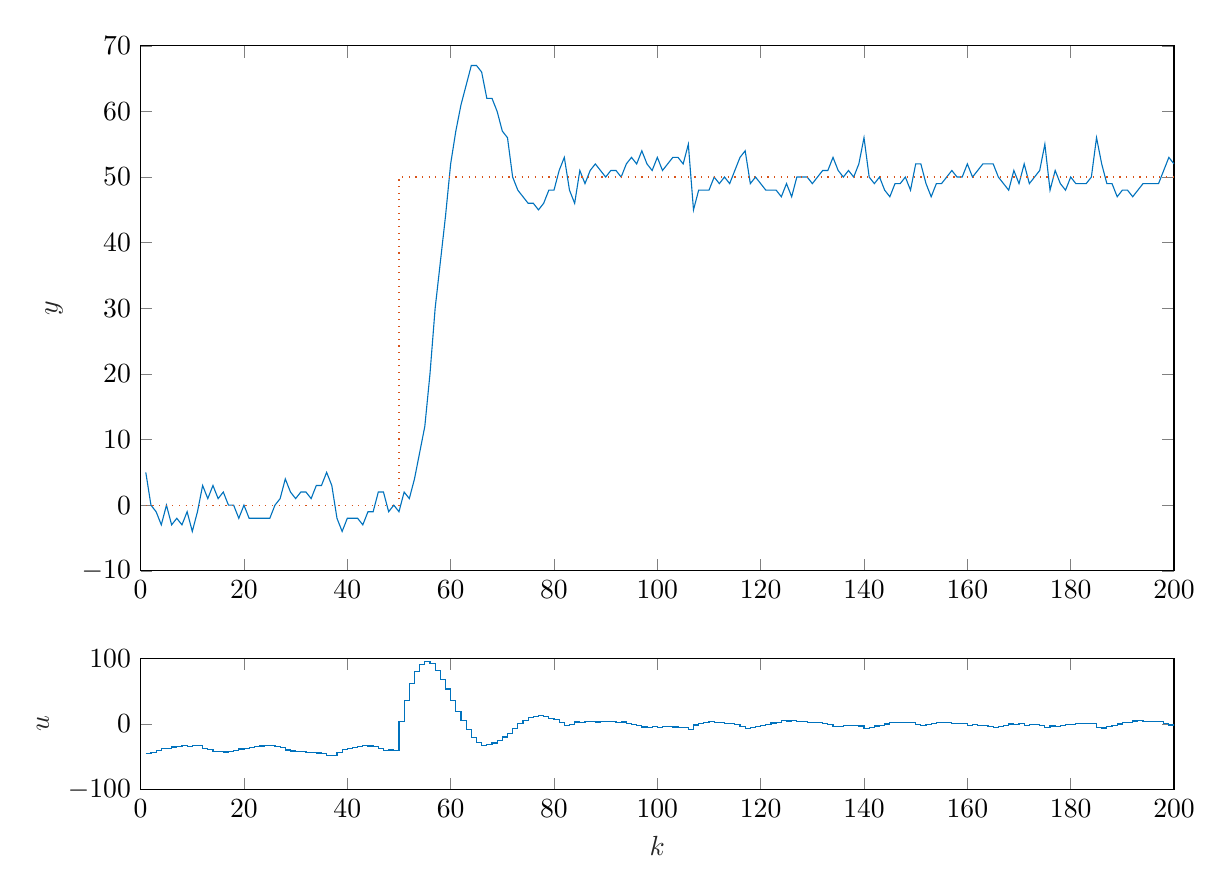
\begin{tikzpicture}

\begin{axis}[%
width=5.167in,
height=0.656in,
at={(0.646in,0.525in)},
scale only axis,
xmin=0,
xmax=200,
xtick={0,20,40,60,80,100,120,140,160,180,200},
xlabel style={font=\color{white!15!black}},
xlabel={$k$},
ymin=-100,
ymax=100,
ytick={-100,0,100},
ylabel style={font=\color{white!15!black}},
ylabel={$u$},
axis background/.style={fill=white}
]
\addplot[const plot, color=mycolor1, forget plot] table[row sep=crcr] {%
1	-45.28\\
2	-43.22\\
3	-40.86\\
4	-37.48\\
5	-37.48\\
6	-35.09\\
7	-34.29\\
8	-33.05\\
9	-33.95\\
10	-32.2\\
11	-33.22\\
12	-37.32\\
13	-38.76\\
14	-41.39\\
15	-41.71\\
16	-42.67\\
17	-41.55\\
18	-40.61\\
19	-38.08\\
20	-37.75\\
21	-35.92\\
22	-34.58\\
23	-33.6\\
24	-32.92\\
25	-32.37\\
26	-33.64\\
27	-35.52\\
28	-39.58\\
29	-41.13\\
30	-41.49\\
31	-42.55\\
32	-43.28\\
33	-42.89\\
34	-44.16\\
35	-45.19\\
36	-47.67\\
37	-48.01\\
38	-44.01\\
39	-39.15\\
40	-36.99\\
41	-35.37\\
42	-34.2\\
43	-32.75\\
44	-33.63\\
45	-34.52\\
46	-37.77\\
47	-40.29\\
48	-39.65\\
49	-39.9\\
50	3.2\\
51	35.18\\
52	61.28\\
53	79.73\\
54	90.88\\
55	95.77\\
56	92.49\\
57	81.76\\
58	68.26\\
59	53.25\\
60	36.01\\
61	19.68\\
62	4.7\\
63	-8.47\\
64	-20.17\\
65	-28.3\\
66	-32.46\\
67	-31.07\\
68	-29.03\\
69	-25.25\\
70	-19.76\\
71	-14.91\\
72	-6.85\\
73	0.35\\
74	5.64\\
75	9.36\\
76	11.21\\
77	12.41\\
78	11.66\\
79	8.87\\
80	6.58\\
81	2.32\\
82	-2\\
83	-0.5\\
84	2.96\\
85	2.15\\
86	3.83\\
87	3.73\\
88	3.1\\
89	3.13\\
90	3.86\\
91	3.5\\
92	2.88\\
93	3.03\\
94	1.38\\
95	-0.95\\
96	-2.07\\
97	-4.55\\
98	-4.88\\
99	-4.06\\
100	-4.94\\
101	-3.85\\
102	-3.73\\
103	-4.58\\
104	-5.36\\
105	-5.23\\
106	-7.83\\
107	-1.56\\
108	0.71\\
109	2.28\\
110	3.4\\
111	2.32\\
112	2.06\\
113	0.82\\
114	0.61\\
115	-1.12\\
116	-3.96\\
117	-6.96\\
118	-4.93\\
119	-4.08\\
120	-2.54\\
121	-0.31\\
122	1.48\\
123	2.85\\
124	4.78\\
125	4.51\\
126	5.88\\
127	4.4\\
128	3.21\\
129	2.23\\
130	2.37\\
131	1.66\\
132	0.2\\
133	-0.87\\
134	-3.36\\
135	-3.6\\
136	-2.84\\
137	-2.94\\
138	-2.15\\
139	-3.03\\
140	-7.1\\
141	-5.34\\
142	-3.11\\
143	-2.31\\
144	-0.06\\
145	2.62\\
146	2.87\\
147	2.88\\
148	1.9\\
149	2.63\\
150	-0.17\\
151	-2.36\\
152	-1.4\\
153	1.17\\
154	1.63\\
155	2.05\\
156	1.62\\
157	0.35\\
158	0.2\\
159	0.09\\
160	-1.67\\
161	-1.28\\
162	-1.71\\
163	-2.94\\
164	-3.93\\
165	-4.72\\
166	-3.76\\
167	-2.16\\
168	-0.04\\
169	-0.91\\
170	0.1\\
171	-1.67\\
172	-0.71\\
173	-0.8\\
174	-1.73\\
175	-5.81\\
176	-3.09\\
177	-3.44\\
178	-2.17\\
179	-0.23\\
180	-0.44\\
181	0.19\\
182	0.66\\
183	0.96\\
184	0.34\\
185	-5.14\\
186	-6.12\\
187	-4.3\\
188	-2.85\\
189	0.05\\
190	1.63\\
191	2.82\\
192	4.48\\
193	4.85\\
194	4.19\\
195	3.68\\
196	3.35\\
197	3.17\\
198	1.42\\
199	-1.54\\
200	-2.97\\
};
\end{axis}

\begin{axis}[%
width=5.167in,
height=2.625in,
at={(0.646in,1.619in)},
scale only axis,
xmin=0,
xmax=200,
xtick={0,20,40,60,80,100,120,140,160,180,200},
ymin=-10,
ymax=70,
ytick={-10,0,10,20,30,40,50,60,70},
ylabel style={font=\color{white!15!black}},
ylabel={$y$},
axis background/.style={fill=white}
]
\addplot [color=mycolor1, forget plot]
  table[row sep=crcr]{%
1	5\\
2	0\\
3	-1\\
4	-3\\
5	0\\
6	-3\\
7	-2\\
8	-3\\
9	-1\\
10	-4\\
11	-1\\
12	3\\
13	1\\
14	3\\
15	1\\
16	2\\
17	0\\
18	0\\
19	-2\\
20	0\\
21	-2\\
22	-2\\
23	-2\\
24	-2\\
25	-2\\
26	0\\
27	1\\
28	4\\
29	2\\
30	1\\
31	2\\
32	2\\
33	1\\
34	3\\
35	3\\
36	5\\
37	3\\
38	-2\\
39	-4\\
40	-2\\
41	-2\\
42	-2\\
43	-3\\
44	-1\\
45	-1\\
46	2\\
47	2\\
48	-1\\
49	0\\
50	-1\\
51	2\\
52	1\\
53	4\\
54	8\\
55	12\\
56	20\\
57	30\\
58	37\\
59	44\\
60	52\\
61	57\\
62	61\\
63	64\\
64	67\\
65	67\\
66	66\\
67	62\\
68	62\\
69	60\\
70	57\\
71	56\\
72	50\\
73	48\\
74	47\\
75	46\\
76	46\\
77	45\\
78	46\\
79	48\\
80	48\\
81	51\\
82	53\\
83	48\\
84	46\\
85	51\\
86	49\\
87	51\\
88	52\\
89	51\\
90	50\\
91	51\\
92	51\\
93	50\\
94	52\\
95	53\\
96	52\\
97	54\\
98	52\\
99	51\\
100	53\\
101	51\\
102	52\\
103	53\\
104	53\\
105	52\\
106	55\\
107	45\\
108	48\\
109	48\\
110	48\\
111	50\\
112	49\\
113	50\\
114	49\\
115	51\\
116	53\\
117	54\\
118	49\\
119	50\\
120	49\\
121	48\\
122	48\\
123	48\\
124	47\\
125	49\\
126	47\\
127	50\\
128	50\\
129	50\\
130	49\\
131	50\\
132	51\\
133	51\\
134	53\\
135	51\\
136	50\\
137	51\\
138	50\\
139	52\\
140	56\\
141	50\\
142	49\\
143	50\\
144	48\\
145	47\\
146	49\\
147	49\\
148	50\\
149	48\\
150	52\\
151	52\\
152	49\\
153	47\\
154	49\\
155	49\\
156	50\\
157	51\\
158	50\\
159	50\\
160	52\\
161	50\\
162	51\\
163	52\\
164	52\\
165	52\\
166	50\\
167	49\\
168	48\\
169	51\\
170	49\\
171	52\\
172	49\\
173	50\\
174	51\\
175	55\\
176	48\\
177	51\\
178	49\\
179	48\\
180	50\\
181	49\\
182	49\\
183	49\\
184	50\\
185	56\\
186	52\\
187	49\\
188	49\\
189	47\\
190	48\\
191	48\\
192	47\\
193	48\\
194	49\\
195	49\\
196	49\\
197	49\\
198	51\\
199	53\\
200	52\\
};
\addplot[const plot, color=mycolor2, dotted, forget plot] table[row sep=crcr] {%
1	0\\
2	0\\
3	0\\
4	0\\
5	0\\
6	0\\
7	0\\
8	0\\
9	0\\
10	0\\
11	0\\
12	0\\
13	0\\
14	0\\
15	0\\
16	0\\
17	0\\
18	0\\
19	0\\
20	0\\
21	0\\
22	0\\
23	0\\
24	0\\
25	0\\
26	0\\
27	0\\
28	0\\
29	0\\
30	0\\
31	0\\
32	0\\
33	0\\
34	0\\
35	0\\
36	0\\
37	0\\
38	0\\
39	0\\
40	0\\
41	0\\
42	0\\
43	0\\
44	0\\
45	0\\
46	0\\
47	0\\
48	0\\
49	0\\
50	50\\
51	50\\
52	50\\
53	50\\
54	50\\
55	50\\
56	50\\
57	50\\
58	50\\
59	50\\
60	50\\
61	50\\
62	50\\
63	50\\
64	50\\
65	50\\
66	50\\
67	50\\
68	50\\
69	50\\
70	50\\
71	50\\
72	50\\
73	50\\
74	50\\
75	50\\
76	50\\
77	50\\
78	50\\
79	50\\
80	50\\
81	50\\
82	50\\
83	50\\
84	50\\
85	50\\
86	50\\
87	50\\
88	50\\
89	50\\
90	50\\
91	50\\
92	50\\
93	50\\
94	50\\
95	50\\
96	50\\
97	50\\
98	50\\
99	50\\
100	50\\
101	50\\
102	50\\
103	50\\
104	50\\
105	50\\
106	50\\
107	50\\
108	50\\
109	50\\
110	50\\
111	50\\
112	50\\
113	50\\
114	50\\
115	50\\
116	50\\
117	50\\
118	50\\
119	50\\
120	50\\
121	50\\
122	50\\
123	50\\
124	50\\
125	50\\
126	50\\
127	50\\
128	50\\
129	50\\
130	50\\
131	50\\
132	50\\
133	50\\
134	50\\
135	50\\
136	50\\
137	50\\
138	50\\
139	50\\
140	50\\
141	50\\
142	50\\
143	50\\
144	50\\
145	50\\
146	50\\
147	50\\
148	50\\
149	50\\
150	50\\
151	50\\
152	50\\
153	50\\
154	50\\
155	50\\
156	50\\
157	50\\
158	50\\
159	50\\
160	50\\
161	50\\
162	50\\
163	50\\
164	50\\
165	50\\
166	50\\
167	50\\
168	50\\
169	50\\
170	50\\
171	50\\
172	50\\
173	50\\
174	50\\
175	50\\
176	50\\
177	50\\
178	50\\
179	50\\
180	50\\
181	50\\
182	50\\
183	50\\
184	50\\
185	50\\
186	50\\
187	50\\
188	50\\
189	50\\
190	50\\
191	50\\
192	50\\
193	50\\
194	50\\
195	50\\
196	50\\
197	50\\
198	50\\
199	50\\
200	50\\
};
\end{axis}
\end{tikzpicture}%
\end{figure}

\begin{figure}[H]
\centering
%err =14746
\definecolor{mycolor1}{rgb}{0.00000,0.44700,0.74100}%
\definecolor{mycolor2}{rgb}{0.85000,0.32500,0.09800}%
%
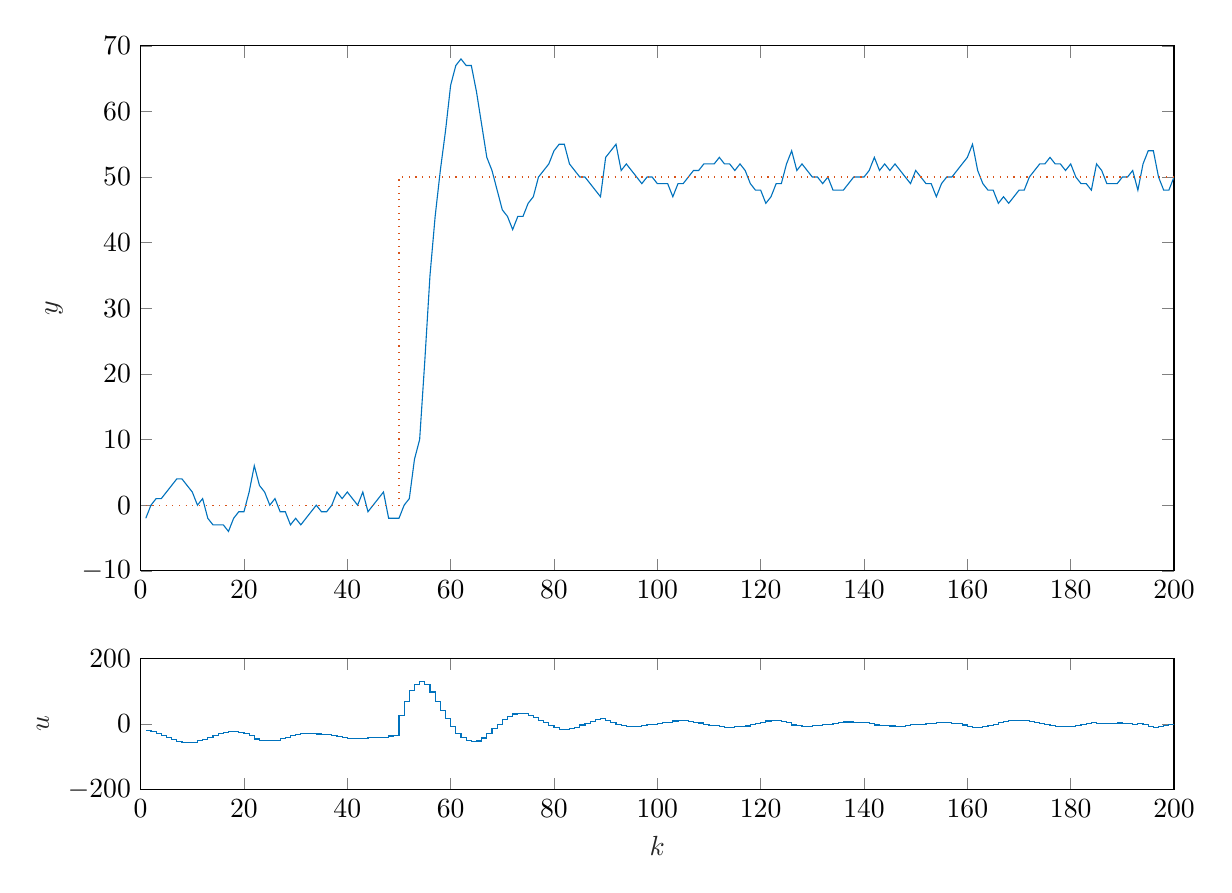
\begin{tikzpicture}

\begin{axis}[%
width=5.167in,
height=0.656in,
at={(0.646in,0.525in)},
scale only axis,
xmin=0,
xmax=200,
xtick={0,20,40,60,80,100,120,140,160,180,200},
xlabel style={font=\color{white!15!black}},
xlabel={$k$},
ymin=-200,
ymax=200,
ytick={-200,0,200},
ylabel style={font=\color{white!15!black}},
ylabel={$u$},
axis background/.style={fill=white}
]
\addplot[const plot, color=mycolor1, forget plot] table[row sep=crcr] {%
1	-19.74\\
2	-23.74\\
3	-29.41\\
4	-34.88\\
5	-40.86\\
6	-46.88\\
7	-52.46\\
8	-56.11\\
9	-56.93\\
10	-55.39\\
11	-50.72\\
12	-47.37\\
13	-40.7\\
14	-34.09\\
15	-29.19\\
16	-25.98\\
17	-23.06\\
18	-24.09\\
19	-26.98\\
20	-29.85\\
21	-36.12\\
22	-45.87\\
23	-49.87\\
24	-51.45\\
25	-49.88\\
26	-49.05\\
27	-45.31\\
28	-41.8\\
29	-36.43\\
30	-33.35\\
31	-29.87\\
32	-28.46\\
33	-28.79\\
34	-30.53\\
35	-31.17\\
36	-32.04\\
37	-34.2\\
38	-38.48\\
39	-40.7\\
40	-43.51\\
41	-44.36\\
42	-43.49\\
43	-44.68\\
44	-41.74\\
45	-40.18\\
46	-39.86\\
47	-40.68\\
48	-36.71\\
49	-33.8\\
50	25.9\\
51	69.61\\
52	101.55\\
53	119.21\\
54	128.47\\
55	120.16\\
56	97.39\\
57	69.77\\
58	42.13\\
59	16.71\\
60	-8.14\\
61	-27.67\\
62	-41.62\\
63	-49.4\\
64	-53.96\\
65	-51.85\\
66	-42.89\\
67	-28.82\\
68	-14.95\\
69	-0.92\\
70	12.35\\
71	22.3\\
72	30.27\\
73	32.22\\
74	31.59\\
75	26.88\\
76	20.87\\
77	11.91\\
78	3.49\\
79	-3.83\\
80	-10.71\\
81	-16.1\\
82	-18.06\\
83	-14.45\\
84	-9.37\\
85	-3.22\\
86	2.28\\
87	7.41\\
88	12.34\\
89	15.98\\
90	10.78\\
91	4.65\\
92	-2.35\\
93	-4.05\\
94	-6.68\\
95	-7.45\\
96	-6.56\\
97	-4\\
98	-2.85\\
99	-1.53\\
100	0.98\\
101	3.19\\
102	5.11\\
103	8.98\\
104	9.66\\
105	9.95\\
106	8.62\\
107	5.83\\
108	3.07\\
109	-0.65\\
110	-3.67\\
111	-5.98\\
112	-8.72\\
113	-9.46\\
114	-9.63\\
115	-8.25\\
116	-7.96\\
117	-6.31\\
118	-2.56\\
119	1.58\\
120	4.66\\
121	9.15\\
122	11.04\\
123	9.71\\
124	8.22\\
125	3.24\\
126	-3.21\\
127	-4.79\\
128	-7.05\\
129	-7.31\\
130	-5.99\\
131	-4.58\\
132	-2.12\\
133	-1.23\\
134	1.76\\
135	4.13\\
136	5.94\\
137	6.16\\
138	5.17\\
139	4.19\\
140	3.24\\
141	1.14\\
142	-3.05\\
143	-3.98\\
144	-5.84\\
145	-6.1\\
146	-7.28\\
147	-6.85\\
148	-5.17\\
149	-2.61\\
150	-2.77\\
151	-1.65\\
152	0.39\\
153	1.89\\
154	5.16\\
155	5.18\\
156	3.84\\
157	2.61\\
158	0.18\\
159	-3.01\\
160	-6.71\\
161	-11.79\\
162	-10.84\\
163	-7.58\\
164	-3.72\\
165	-0.41\\
166	4.6\\
167	7.28\\
168	10.33\\
169	11.27\\
170	10.69\\
171	10.18\\
172	7.4\\
173	4.02\\
174	0.21\\
175	-2.65\\
176	-5.99\\
177	-7.33\\
178	-8.18\\
179	-7.42\\
180	-7.69\\
181	-5.32\\
182	-2.25\\
183	0.19\\
184	3.27\\
185	0.98\\
186	0.21\\
187	1.7\\
188	2.49\\
189	2.86\\
190	1.86\\
191	0.91\\
192	-1.09\\
193	0.62\\
194	-2.67\\
195	-7.37\\
196	-10.76\\
197	-8.51\\
198	-4.16\\
199	-0.62\\
200	0.14\\
};
\end{axis}

\begin{axis}[%
width=5.167in,
height=2.625in,
at={(0.646in,1.619in)},
scale only axis,
xmin=0,
xmax=200,
xtick={0,20,40,60,80,100,120,140,160,180,200},
ymin=-10,
ymax=70,
ytick={-10,0,10,20,30,40,50,60,70},
ylabel style={font=\color{white!15!black}},
ylabel={$y$},
axis background/.style={fill=white}
]
\addplot [color=mycolor1, forget plot]
  table[row sep=crcr]{%
1	-2\\
2	0\\
3	1\\
4	1\\
5	2\\
6	3\\
7	4\\
8	4\\
9	3\\
10	2\\
11	0\\
12	1\\
13	-2\\
14	-3\\
15	-3\\
16	-3\\
17	-4\\
18	-2\\
19	-1\\
20	-1\\
21	2\\
22	6\\
23	3\\
24	2\\
25	0\\
26	1\\
27	-1\\
28	-1\\
29	-3\\
30	-2\\
31	-3\\
32	-2\\
33	-1\\
34	0\\
35	-1\\
36	-1\\
37	0\\
38	2\\
39	1\\
40	2\\
41	1\\
42	0\\
43	2\\
44	-1\\
45	0\\
46	1\\
47	2\\
48	-2\\
49	-2\\
50	-2\\
51	0\\
52	1\\
53	7\\
54	10\\
55	22\\
56	35\\
57	44\\
58	51\\
59	57\\
60	64\\
61	67\\
62	68\\
63	67\\
64	67\\
65	63\\
66	58\\
67	53\\
68	51\\
69	48\\
70	45\\
71	44\\
72	42\\
73	44\\
74	44\\
75	46\\
76	47\\
77	50\\
78	51\\
79	52\\
80	54\\
81	55\\
82	55\\
83	52\\
84	51\\
85	50\\
86	50\\
87	49\\
88	48\\
89	47\\
90	53\\
91	54\\
92	55\\
93	51\\
94	52\\
95	51\\
96	50\\
97	49\\
98	50\\
99	50\\
100	49\\
101	49\\
102	49\\
103	47\\
104	49\\
105	49\\
106	50\\
107	51\\
108	51\\
109	52\\
110	52\\
111	52\\
112	53\\
113	52\\
114	52\\
115	51\\
116	52\\
117	51\\
118	49\\
119	48\\
120	48\\
121	46\\
122	47\\
123	49\\
124	49\\
125	52\\
126	54\\
127	51\\
128	52\\
129	51\\
130	50\\
131	50\\
132	49\\
133	50\\
134	48\\
135	48\\
136	48\\
137	49\\
138	50\\
139	50\\
140	50\\
141	51\\
142	53\\
143	51\\
144	52\\
145	51\\
146	52\\
147	51\\
148	50\\
149	49\\
150	51\\
151	50\\
152	49\\
153	49\\
154	47\\
155	49\\
156	50\\
157	50\\
158	51\\
159	52\\
160	53\\
161	55\\
162	51\\
163	49\\
164	48\\
165	48\\
166	46\\
167	47\\
168	46\\
169	47\\
170	48\\
171	48\\
172	50\\
173	51\\
174	52\\
175	52\\
176	53\\
177	52\\
178	52\\
179	51\\
180	52\\
181	50\\
182	49\\
183	49\\
184	48\\
185	52\\
186	51\\
187	49\\
188	49\\
189	49\\
190	50\\
191	50\\
192	51\\
193	48\\
194	52\\
195	54\\
196	54\\
197	50\\
198	48\\
199	48\\
200	50\\
};
\addplot[const plot, color=mycolor2, dotted, forget plot] table[row sep=crcr] {%
1	0\\
2	0\\
3	0\\
4	0\\
5	0\\
6	0\\
7	0\\
8	0\\
9	0\\
10	0\\
11	0\\
12	0\\
13	0\\
14	0\\
15	0\\
16	0\\
17	0\\
18	0\\
19	0\\
20	0\\
21	0\\
22	0\\
23	0\\
24	0\\
25	0\\
26	0\\
27	0\\
28	0\\
29	0\\
30	0\\
31	0\\
32	0\\
33	0\\
34	0\\
35	0\\
36	0\\
37	0\\
38	0\\
39	0\\
40	0\\
41	0\\
42	0\\
43	0\\
44	0\\
45	0\\
46	0\\
47	0\\
48	0\\
49	0\\
50	50\\
51	50\\
52	50\\
53	50\\
54	50\\
55	50\\
56	50\\
57	50\\
58	50\\
59	50\\
60	50\\
61	50\\
62	50\\
63	50\\
64	50\\
65	50\\
66	50\\
67	50\\
68	50\\
69	50\\
70	50\\
71	50\\
72	50\\
73	50\\
74	50\\
75	50\\
76	50\\
77	50\\
78	50\\
79	50\\
80	50\\
81	50\\
82	50\\
83	50\\
84	50\\
85	50\\
86	50\\
87	50\\
88	50\\
89	50\\
90	50\\
91	50\\
92	50\\
93	50\\
94	50\\
95	50\\
96	50\\
97	50\\
98	50\\
99	50\\
100	50\\
101	50\\
102	50\\
103	50\\
104	50\\
105	50\\
106	50\\
107	50\\
108	50\\
109	50\\
110	50\\
111	50\\
112	50\\
113	50\\
114	50\\
115	50\\
116	50\\
117	50\\
118	50\\
119	50\\
120	50\\
121	50\\
122	50\\
123	50\\
124	50\\
125	50\\
126	50\\
127	50\\
128	50\\
129	50\\
130	50\\
131	50\\
132	50\\
133	50\\
134	50\\
135	50\\
136	50\\
137	50\\
138	50\\
139	50\\
140	50\\
141	50\\
142	50\\
143	50\\
144	50\\
145	50\\
146	50\\
147	50\\
148	50\\
149	50\\
150	50\\
151	50\\
152	50\\
153	50\\
154	50\\
155	50\\
156	50\\
157	50\\
158	50\\
159	50\\
160	50\\
161	50\\
162	50\\
163	50\\
164	50\\
165	50\\
166	50\\
167	50\\
168	50\\
169	50\\
170	50\\
171	50\\
172	50\\
173	50\\
174	50\\
175	50\\
176	50\\
177	50\\
178	50\\
179	50\\
180	50\\
181	50\\
182	50\\
183	50\\
184	50\\
185	50\\
186	50\\
187	50\\
188	50\\
189	50\\
190	50\\
191	50\\
192	50\\
193	50\\
194	50\\
195	50\\
196	50\\
197	50\\
198	50\\
199	50\\
200	50\\
};
\end{axis}
\end{tikzpicture}%
\end{figure}

\begin{figure}[H]
\centering
%err =29438
\definecolor{mycolor1}{rgb}{0.00000,0.44700,0.74100}%
\definecolor{mycolor2}{rgb}{0.85000,0.32500,0.09800}%
%
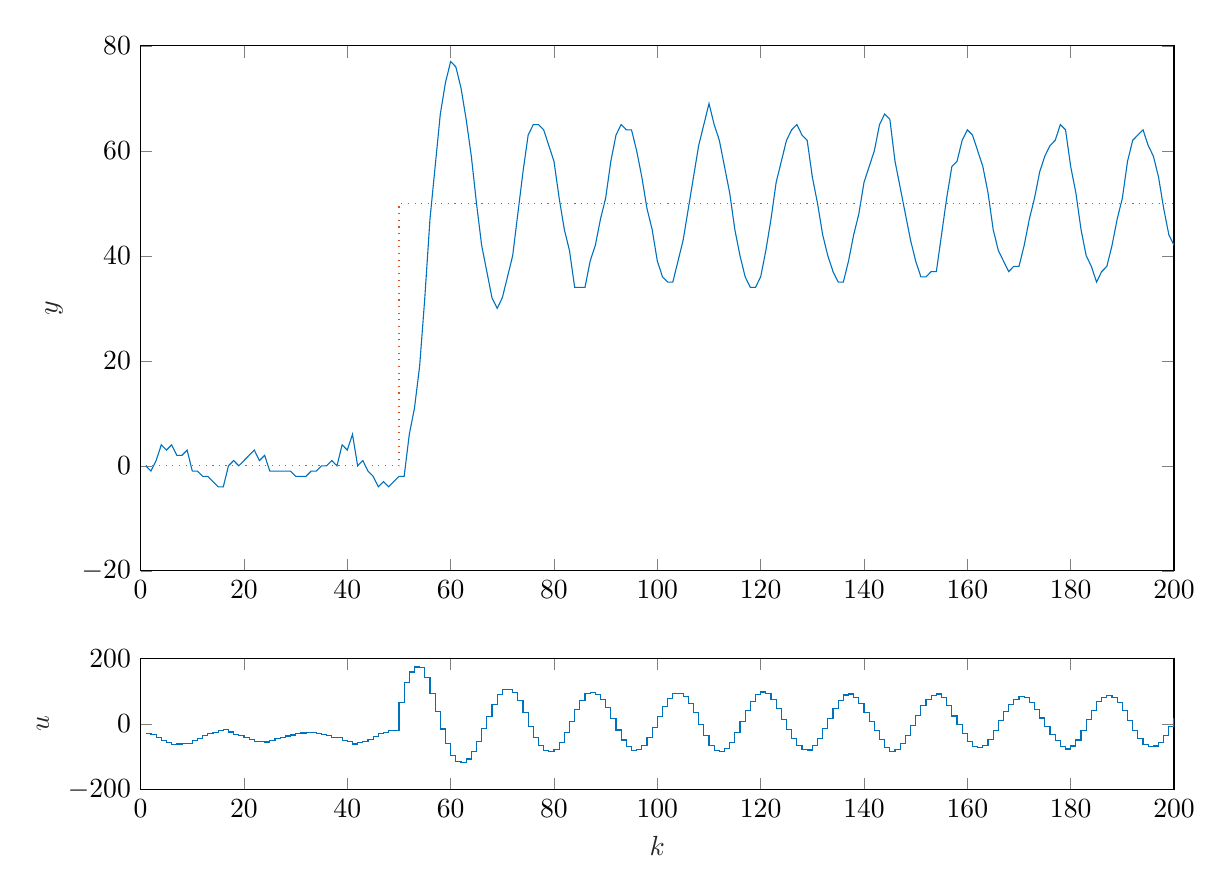
\begin{tikzpicture}

\begin{axis}[%
width=5.167in,
height=0.656in,
at={(0.646in,0.525in)},
scale only axis,
xmin=0,
xmax=200,
xtick={0,20,40,60,80,100,120,140,160,180,200},
xlabel style={font=\color{white!15!black}},
xlabel={$k$},
ymin=-200,
ymax=200,
ytick={-200,0,200},
ylabel style={font=\color{white!15!black}},
ylabel={$u$},
axis background/.style={fill=white}
]
\addplot[const plot, color=mycolor1, forget plot] table[row sep=crcr] {%
1	-29.42\\
2	-33.08\\
3	-40.13\\
4	-50.68\\
5	-56.22\\
6	-61.43\\
7	-61.06\\
8	-59.64\\
9	-58.93\\
10	-50.27\\
11	-42.82\\
12	-35.49\\
13	-30.01\\
14	-24.61\\
15	-20.01\\
16	-17.79\\
17	-24.17\\
18	-31.59\\
19	-36.09\\
20	-41.72\\
21	-47.88\\
22	-53.81\\
23	-53.82\\
24	-54.66\\
25	-49.42\\
26	-44.62\\
27	-40.37\\
28	-36.65\\
29	-33.59\\
30	-29.88\\
31	-27.43\\
32	-26.03\\
33	-27.16\\
34	-28.66\\
35	-32.15\\
36	-35.46\\
37	-39.94\\
38	-41.76\\
39	-49.74\\
40	-53.62\\
41	-61.01\\
42	-55.43\\
43	-52.15\\
44	-45.85\\
45	-38.7\\
46	-29.54\\
47	-24.75\\
48	-20.04\\
49	-19.09\\
50	64.63\\
51	126.99\\
52	158.44\\
53	173.83\\
54	171\\
55	143.17\\
56	93.6\\
57	39.53\\
58	-15.02\\
59	-60.42\\
60	-95.64\\
61	-114.45\\
62	-117.61\\
63	-106.72\\
64	-84.95\\
65	-53.14\\
66	-14.42\\
67	23.83\\
68	60.66\\
69	89.88\\
70	105.05\\
71	105.82\\
72	95.57\\
73	70.66\\
74	34.89\\
75	-6.44\\
76	-41.16\\
77	-66.49\\
78	-81.57\\
79	-84.56\\
80	-77.2\\
81	-56.27\\
82	-25.54\\
83	7.16\\
84	44.3\\
85	72.52\\
86	92.82\\
87	96.36\\
88	90.92\\
89	73.52\\
90	49.51\\
91	16.97\\
92	-18.34\\
93	-48.7\\
94	-67.98\\
95	-79.8\\
96	-78.76\\
97	-64.73\\
98	-40.11\\
99	-11.61\\
100	22.14\\
101	53.2\\
102	77.15\\
103	92.73\\
104	94.36\\
105	84.87\\
106	63.7\\
107	34.26\\
108	-0.51\\
109	-34.44\\
110	-66.32\\
111	-81.64\\
112	-85\\
113	-75.41\\
114	-55.65\\
115	-25.47\\
116	8.3\\
117	41.52\\
118	69.53\\
119	89.01\\
120	97.75\\
121	92.4\\
122	74.73\\
123	46.07\\
124	15.01\\
125	-16.89\\
126	-44.59\\
127	-66.13\\
128	-76.47\\
129	-79.3\\
130	-65.95\\
131	-43.99\\
132	-14.36\\
133	16.84\\
134	46.39\\
135	71.61\\
136	88.57\\
137	91.5\\
138	81.61\\
139	63.65\\
140	36.45\\
141	8.57\\
142	-18.78\\
143	-47.54\\
144	-70.95\\
145	-84.28\\
146	-77.47\\
147	-60.21\\
148	-35.33\\
149	-4.89\\
150	26.64\\
151	55.55\\
152	75.83\\
153	86.76\\
154	91.61\\
155	79.77\\
156	55.5\\
157	24.43\\
158	-2.3\\
159	-30.14\\
160	-53.97\\
161	-68.36\\
162	-70.87\\
163	-64.21\\
164	-47.31\\
165	-19.57\\
166	10.18\\
167	37.01\\
168	60.64\\
169	75.3\\
170	83.8\\
171	80.29\\
172	65.71\\
173	44.81\\
174	18.28\\
175	-8.38\\
176	-32.19\\
177	-50.81\\
178	-67.99\\
179	-76.22\\
180	-67.14\\
181	-48.56\\
182	-19.81\\
183	12.53\\
184	41.33\\
185	67.43\\
186	81.74\\
187	87.56\\
188	81.39\\
189	64.68\\
190	42.53\\
191	12.06\\
192	-18.57\\
193	-42.92\\
194	-61.55\\
195	-68.41\\
196	-67.07\\
197	-55.95\\
198	-34.01\\
199	-6.5\\
200	18.85\\
};
\end{axis}

\begin{axis}[%
width=5.167in,
height=2.625in,
at={(0.646in,1.619in)},
scale only axis,
xmin=0,
xmax=200,
xtick={0,20,40,60,80,100,120,140,160,180,200},
ymin=-20,
ymax=80,
ytick={-20,0,20,40,60,80},
ylabel style={font=\color{white!15!black}},
ylabel={$y$},
axis background/.style={fill=white}
]
\addplot [color=mycolor1, forget plot]
  table[row sep=crcr]{%
1	0\\
2	-1\\
3	1\\
4	4\\
5	3\\
6	4\\
7	2\\
8	2\\
9	3\\
10	-1\\
11	-1\\
12	-2\\
13	-2\\
14	-3\\
15	-4\\
16	-4\\
17	0\\
18	1\\
19	0\\
20	1\\
21	2\\
22	3\\
23	1\\
24	2\\
25	-1\\
26	-1\\
27	-1\\
28	-1\\
29	-1\\
30	-2\\
31	-2\\
32	-2\\
33	-1\\
34	-1\\
35	0\\
36	0\\
37	1\\
38	0\\
39	4\\
40	3\\
41	6\\
42	0\\
43	1\\
44	-1\\
45	-2\\
46	-4\\
47	-3\\
48	-4\\
49	-3\\
50	-2\\
51	-2\\
52	6\\
53	11\\
54	19\\
55	32\\
56	47\\
57	57\\
58	67\\
59	73\\
60	77\\
61	76\\
62	72\\
63	66\\
64	59\\
65	50\\
66	42\\
67	37\\
68	32\\
69	30\\
70	32\\
71	36\\
72	40\\
73	48\\
74	56\\
75	63\\
76	65\\
77	65\\
78	64\\
79	61\\
80	58\\
81	51\\
82	45\\
83	41\\
84	34\\
85	34\\
86	34\\
87	39\\
88	42\\
89	47\\
90	51\\
91	58\\
92	63\\
93	65\\
94	64\\
95	64\\
96	60\\
97	55\\
98	49\\
99	45\\
100	39\\
101	36\\
102	35\\
103	35\\
104	39\\
105	43\\
106	49\\
107	55\\
108	61\\
109	65\\
110	69\\
111	65\\
112	62\\
113	57\\
114	52\\
115	45\\
116	40\\
117	36\\
118	34\\
119	34\\
120	36\\
121	41\\
122	47\\
123	54\\
124	58\\
125	62\\
126	64\\
127	65\\
128	63\\
129	62\\
130	55\\
131	50\\
132	44\\
133	40\\
134	37\\
135	35\\
136	35\\
137	39\\
138	44\\
139	48\\
140	54\\
141	57\\
142	60\\
143	65\\
144	67\\
145	66\\
146	58\\
147	53\\
148	48\\
149	43\\
150	39\\
151	36\\
152	36\\
153	37\\
154	37\\
155	44\\
156	51\\
157	57\\
158	58\\
159	62\\
160	64\\
161	63\\
162	60\\
163	57\\
164	52\\
165	45\\
166	41\\
167	39\\
168	37\\
169	38\\
170	38\\
171	42\\
172	47\\
173	51\\
174	56\\
175	59\\
176	61\\
177	62\\
178	65\\
179	64\\
180	57\\
181	52\\
182	45\\
183	40\\
184	38\\
185	35\\
186	37\\
187	38\\
188	42\\
189	47\\
190	51\\
191	58\\
192	62\\
193	63\\
194	64\\
195	61\\
196	59\\
197	55\\
198	49\\
199	44\\
200	42\\
};
\addplot[const plot, color=mycolor2, dotted, forget plot] table[row sep=crcr] {%
1	0\\
2	0\\
3	0\\
4	0\\
5	0\\
6	0\\
7	0\\
8	0\\
9	0\\
10	0\\
11	0\\
12	0\\
13	0\\
14	0\\
15	0\\
16	0\\
17	0\\
18	0\\
19	0\\
20	0\\
21	0\\
22	0\\
23	0\\
24	0\\
25	0\\
26	0\\
27	0\\
28	0\\
29	0\\
30	0\\
31	0\\
32	0\\
33	0\\
34	0\\
35	0\\
36	0\\
37	0\\
38	0\\
39	0\\
40	0\\
41	0\\
42	0\\
43	0\\
44	0\\
45	0\\
46	0\\
47	0\\
48	0\\
49	0\\
50	50\\
51	50\\
52	50\\
53	50\\
54	50\\
55	50\\
56	50\\
57	50\\
58	50\\
59	50\\
60	50\\
61	50\\
62	50\\
63	50\\
64	50\\
65	50\\
66	50\\
67	50\\
68	50\\
69	50\\
70	50\\
71	50\\
72	50\\
73	50\\
74	50\\
75	50\\
76	50\\
77	50\\
78	50\\
79	50\\
80	50\\
81	50\\
82	50\\
83	50\\
84	50\\
85	50\\
86	50\\
87	50\\
88	50\\
89	50\\
90	50\\
91	50\\
92	50\\
93	50\\
94	50\\
95	50\\
96	50\\
97	50\\
98	50\\
99	50\\
100	50\\
101	50\\
102	50\\
103	50\\
104	50\\
105	50\\
106	50\\
107	50\\
108	50\\
109	50\\
110	50\\
111	50\\
112	50\\
113	50\\
114	50\\
115	50\\
116	50\\
117	50\\
118	50\\
119	50\\
120	50\\
121	50\\
122	50\\
123	50\\
124	50\\
125	50\\
126	50\\
127	50\\
128	50\\
129	50\\
130	50\\
131	50\\
132	50\\
133	50\\
134	50\\
135	50\\
136	50\\
137	50\\
138	50\\
139	50\\
140	50\\
141	50\\
142	50\\
143	50\\
144	50\\
145	50\\
146	50\\
147	50\\
148	50\\
149	50\\
150	50\\
151	50\\
152	50\\
153	50\\
154	50\\
155	50\\
156	50\\
157	50\\
158	50\\
159	50\\
160	50\\
161	50\\
162	50\\
163	50\\
164	50\\
165	50\\
166	50\\
167	50\\
168	50\\
169	50\\
170	50\\
171	50\\
172	50\\
173	50\\
174	50\\
175	50\\
176	50\\
177	50\\
178	50\\
179	50\\
180	50\\
181	50\\
182	50\\
183	50\\
184	50\\
185	50\\
186	50\\
187	50\\
188	50\\
189	50\\
190	50\\
191	50\\
192	50\\
193	50\\
194	50\\
195	50\\
196	50\\
197	50\\
198	50\\
199	50\\
200	50\\
};
\end{axis}
\end{tikzpicture}%
\end{figure}

\begin{figure}[H]
\centering
%err =15016
\definecolor{mycolor1}{rgb}{0.00000,0.44700,0.74100}%
\definecolor{mycolor2}{rgb}{0.85000,0.32500,0.09800}%
%
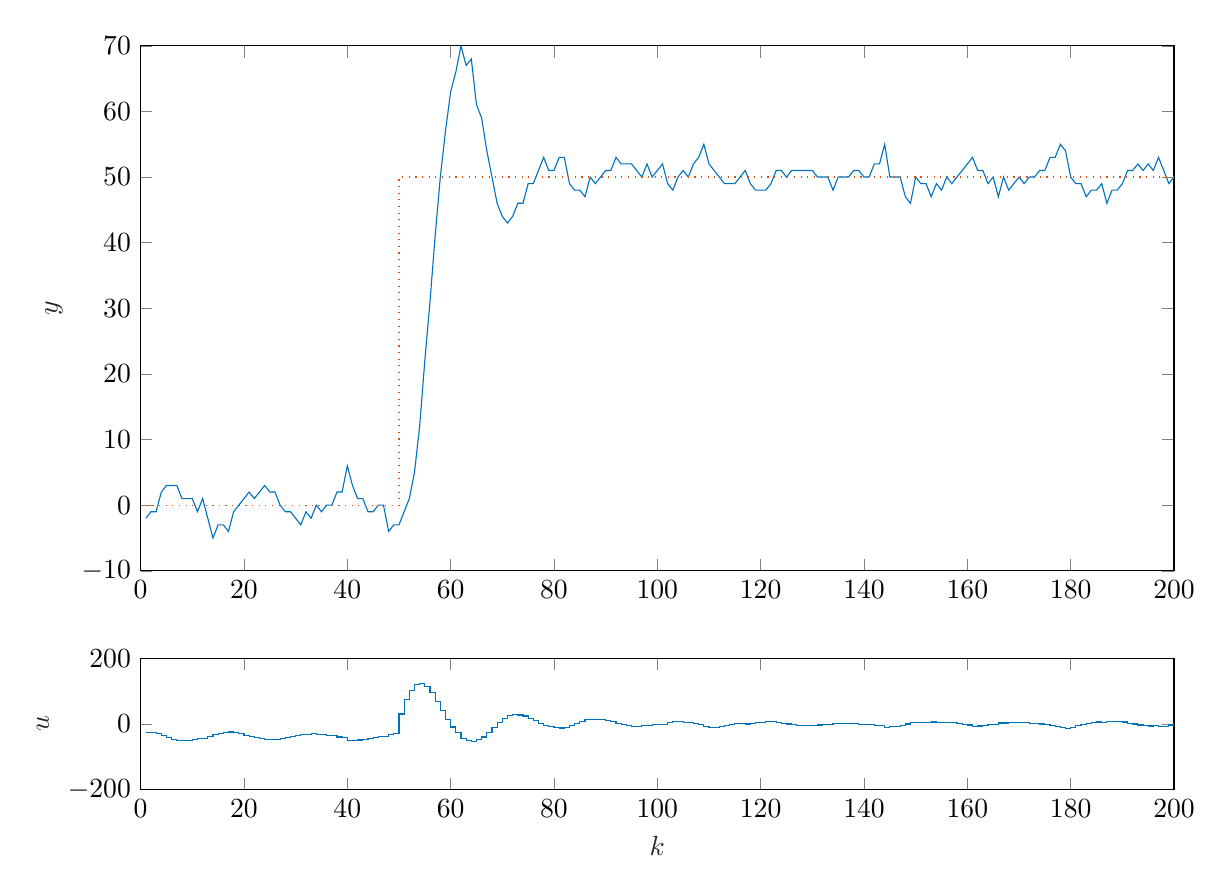
\begin{tikzpicture}

\begin{axis}[%
width=5.167in,
height=0.656in,
at={(0.646in,0.525in)},
scale only axis,
xmin=0,
xmax=200,
xtick={0,20,40,60,80,100,120,140,160,180,200},
xlabel style={font=\color{white!15!black}},
xlabel={$k$},
ymin=-200,
ymax=200,
ytick={-200,0,200},
ylabel style={font=\color{white!15!black}},
ylabel={$u$},
axis background/.style={fill=white}
]
\addplot[const plot, color=mycolor1, forget plot] table[row sep=crcr] {%
1	-25.5\\
2	-27.28\\
3	-29.54\\
4	-35.52\\
5	-41.65\\
6	-46.4\\
7	-49.9\\
8	-49.79\\
9	-49.12\\
10	-48.07\\
11	-44.26\\
12	-43.26\\
13	-38.83\\
14	-31.78\\
15	-28.79\\
16	-26.84\\
17	-24.31\\
18	-26.52\\
19	-29.96\\
20	-34.08\\
21	-38.74\\
22	-41.26\\
23	-44.12\\
24	-47.13\\
25	-47.85\\
26	-47.89\\
27	-45.26\\
28	-41.81\\
29	-38.86\\
30	-35.27\\
31	-31.35\\
32	-30.88\\
33	-29.71\\
34	-31.53\\
35	-32.11\\
36	-34.08\\
37	-35.83\\
38	-39.55\\
39	-42.38\\
40	-49.09\\
41	-50.49\\
42	-48.95\\
43	-47.44\\
44	-43.54\\
45	-40.26\\
46	-38.75\\
47	-37.76\\
48	-32.59\\
49	-30.12\\
50	30.29\\
51	73.46\\
52	103.01\\
53	120.47\\
54	124.64\\
55	114.36\\
56	94.71\\
57	68.66\\
58	40.48\\
59	14.32\\
60	-9.17\\
61	-27.19\\
62	-43.09\\
63	-49.55\\
64	-53.98\\
65	-48.09\\
66	-39.79\\
67	-26.56\\
68	-11.48\\
69	4.11\\
70	16.68\\
71	25.64\\
72	29.09\\
73	27.5\\
74	24.37\\
75	16.71\\
76	10.05\\
77	2.33\\
78	-5.83\\
79	-8.93\\
80	-10.11\\
81	-12.4\\
82	-12.07\\
83	-5.71\\
84	0.97\\
85	6.74\\
86	12.77\\
87	13.31\\
88	14.71\\
89	13.21\\
90	9.82\\
91	6.58\\
92	0.92\\
93	-2.63\\
94	-5.16\\
95	-6.83\\
96	-6.56\\
97	-4.27\\
98	-4.47\\
99	-1.68\\
100	-0.31\\
101	-0.26\\
102	3.29\\
103	6.99\\
104	6.98\\
105	5.33\\
106	4.82\\
107	1.44\\
108	-2.91\\
109	-8.84\\
110	-9.92\\
111	-9.41\\
112	-7.52\\
113	-4.62\\
114	-2.04\\
115	0.18\\
116	0.72\\
117	-0.11\\
118	1.58\\
119	3.96\\
120	5.73\\
121	6.99\\
122	6.52\\
123	3.55\\
124	0.96\\
125	-0.17\\
126	-2.24\\
127	-3.69\\
128	-4.46\\
129	-4.58\\
130	-4.48\\
131	-3.03\\
132	-1.78\\
133	-0.86\\
134	2.25\\
135	2.27\\
136	2.07\\
137	1.82\\
138	0.26\\
139	-1.23\\
140	-1.29\\
141	-1.42\\
142	-3.88\\
143	-5.64\\
144	-10.44\\
145	-8.21\\
146	-6.39\\
147	-4.94\\
148	-0.08\\
149	4.87\\
150	3.85\\
151	4.07\\
152	4\\
153	5.99\\
154	4.99\\
155	5.36\\
156	3.43\\
157	3.24\\
158	1.86\\
159	-0.39\\
160	-3.25\\
161	-6.47\\
162	-6.25\\
163	-5.83\\
164	-2.89\\
165	-1.61\\
166	3.04\\
167	2.91\\
168	4.94\\
169	5.17\\
170	3.86\\
171	3.93\\
172	2.76\\
173	1.75\\
174	-0.19\\
175	-1.57\\
176	-5.06\\
177	-7.62\\
178	-11.75\\
179	-13.61\\
180	-10.04\\
181	-5.89\\
182	-2.75\\
183	2.12\\
184	4.52\\
185	6\\
186	5.55\\
187	8.43\\
188	7.94\\
189	7.57\\
190	6.11\\
191	2.63\\
192	0.01\\
193	-3.14\\
194	-4.25\\
195	-6.07\\
196	-5.89\\
197	-7.79\\
198	-6.52\\
199	-3.07\\
200	-1.6\\
};
\end{axis}

\begin{axis}[%
width=5.167in,
height=2.625in,
at={(0.646in,1.619in)},
scale only axis,
xmin=0,
xmax=200,
xtick={0,20,40,60,80,100,120,140,160,180,200},
ymin=-10,
ymax=70,
ytick={-10,0,10,20,30,40,50,60,70},
ylabel style={font=\color{white!15!black}},
ylabel={$y$},
axis background/.style={fill=white}
]
\addplot [color=mycolor1, forget plot]
  table[row sep=crcr]{%
1	-2\\
2	-1\\
3	-1\\
4	2\\
5	3\\
6	3\\
7	3\\
8	1\\
9	1\\
10	1\\
11	-1\\
12	1\\
13	-2\\
14	-5\\
15	-3\\
16	-3\\
17	-4\\
18	-1\\
19	0\\
20	1\\
21	2\\
22	1\\
23	2\\
24	3\\
25	2\\
26	2\\
27	0\\
28	-1\\
29	-1\\
30	-2\\
31	-3\\
32	-1\\
33	-2\\
34	0\\
35	-1\\
36	0\\
37	0\\
38	2\\
39	2\\
40	6\\
41	3\\
42	1\\
43	1\\
44	-1\\
45	-1\\
46	0\\
47	0\\
48	-4\\
49	-3\\
50	-3\\
51	-1\\
52	1\\
53	5\\
54	12\\
55	22\\
56	31\\
57	41\\
58	50\\
59	57\\
60	63\\
61	66\\
62	70\\
63	67\\
64	68\\
65	61\\
66	59\\
67	54\\
68	50\\
69	46\\
70	44\\
71	43\\
72	44\\
73	46\\
74	46\\
75	49\\
76	49\\
77	51\\
78	53\\
79	51\\
80	51\\
81	53\\
82	53\\
83	49\\
84	48\\
85	48\\
86	47\\
87	50\\
88	49\\
89	50\\
90	51\\
91	51\\
92	53\\
93	52\\
94	52\\
95	52\\
96	51\\
97	50\\
98	52\\
99	50\\
100	51\\
101	52\\
102	49\\
103	48\\
104	50\\
105	51\\
106	50\\
107	52\\
108	53\\
109	55\\
110	52\\
111	51\\
112	50\\
113	49\\
114	49\\
115	49\\
116	50\\
117	51\\
118	49\\
119	48\\
120	48\\
121	48\\
122	49\\
123	51\\
124	51\\
125	50\\
126	51\\
127	51\\
128	51\\
129	51\\
130	51\\
131	50\\
132	50\\
133	50\\
134	48\\
135	50\\
136	50\\
137	50\\
138	51\\
139	51\\
140	50\\
141	50\\
142	52\\
143	52\\
144	55\\
145	50\\
146	50\\
147	50\\
148	47\\
149	46\\
150	50\\
151	49\\
152	49\\
153	47\\
154	49\\
155	48\\
156	50\\
157	49\\
158	50\\
159	51\\
160	52\\
161	53\\
162	51\\
163	51\\
164	49\\
165	50\\
166	47\\
167	50\\
168	48\\
169	49\\
170	50\\
171	49\\
172	50\\
173	50\\
174	51\\
175	51\\
176	53\\
177	53\\
178	55\\
179	54\\
180	50\\
181	49\\
182	49\\
183	47\\
184	48\\
185	48\\
186	49\\
187	46\\
188	48\\
189	48\\
190	49\\
191	51\\
192	51\\
193	52\\
194	51\\
195	52\\
196	51\\
197	53\\
198	51\\
199	49\\
200	50\\
};
\addplot[const plot, color=mycolor2, dotted, forget plot] table[row sep=crcr] {%
1	0\\
2	0\\
3	0\\
4	0\\
5	0\\
6	0\\
7	0\\
8	0\\
9	0\\
10	0\\
11	0\\
12	0\\
13	0\\
14	0\\
15	0\\
16	0\\
17	0\\
18	0\\
19	0\\
20	0\\
21	0\\
22	0\\
23	0\\
24	0\\
25	0\\
26	0\\
27	0\\
28	0\\
29	0\\
30	0\\
31	0\\
32	0\\
33	0\\
34	0\\
35	0\\
36	0\\
37	0\\
38	0\\
39	0\\
40	0\\
41	0\\
42	0\\
43	0\\
44	0\\
45	0\\
46	0\\
47	0\\
48	0\\
49	0\\
50	50\\
51	50\\
52	50\\
53	50\\
54	50\\
55	50\\
56	50\\
57	50\\
58	50\\
59	50\\
60	50\\
61	50\\
62	50\\
63	50\\
64	50\\
65	50\\
66	50\\
67	50\\
68	50\\
69	50\\
70	50\\
71	50\\
72	50\\
73	50\\
74	50\\
75	50\\
76	50\\
77	50\\
78	50\\
79	50\\
80	50\\
81	50\\
82	50\\
83	50\\
84	50\\
85	50\\
86	50\\
87	50\\
88	50\\
89	50\\
90	50\\
91	50\\
92	50\\
93	50\\
94	50\\
95	50\\
96	50\\
97	50\\
98	50\\
99	50\\
100	50\\
101	50\\
102	50\\
103	50\\
104	50\\
105	50\\
106	50\\
107	50\\
108	50\\
109	50\\
110	50\\
111	50\\
112	50\\
113	50\\
114	50\\
115	50\\
116	50\\
117	50\\
118	50\\
119	50\\
120	50\\
121	50\\
122	50\\
123	50\\
124	50\\
125	50\\
126	50\\
127	50\\
128	50\\
129	50\\
130	50\\
131	50\\
132	50\\
133	50\\
134	50\\
135	50\\
136	50\\
137	50\\
138	50\\
139	50\\
140	50\\
141	50\\
142	50\\
143	50\\
144	50\\
145	50\\
146	50\\
147	50\\
148	50\\
149	50\\
150	50\\
151	50\\
152	50\\
153	50\\
154	50\\
155	50\\
156	50\\
157	50\\
158	50\\
159	50\\
160	50\\
161	50\\
162	50\\
163	50\\
164	50\\
165	50\\
166	50\\
167	50\\
168	50\\
169	50\\
170	50\\
171	50\\
172	50\\
173	50\\
174	50\\
175	50\\
176	50\\
177	50\\
178	50\\
179	50\\
180	50\\
181	50\\
182	50\\
183	50\\
184	50\\
185	50\\
186	50\\
187	50\\
188	50\\
189	50\\
190	50\\
191	50\\
192	50\\
193	50\\
194	50\\
195	50\\
196	50\\
197	50\\
198	50\\
199	50\\
200	50\\
};
\end{axis}
\end{tikzpicture}%
\end{figure}

\begin{figure}[H]
\centering
%err =15716
\definecolor{mycolor1}{rgb}{0.00000,0.44700,0.74100}%
\definecolor{mycolor2}{rgb}{0.85000,0.32500,0.09800}%
%
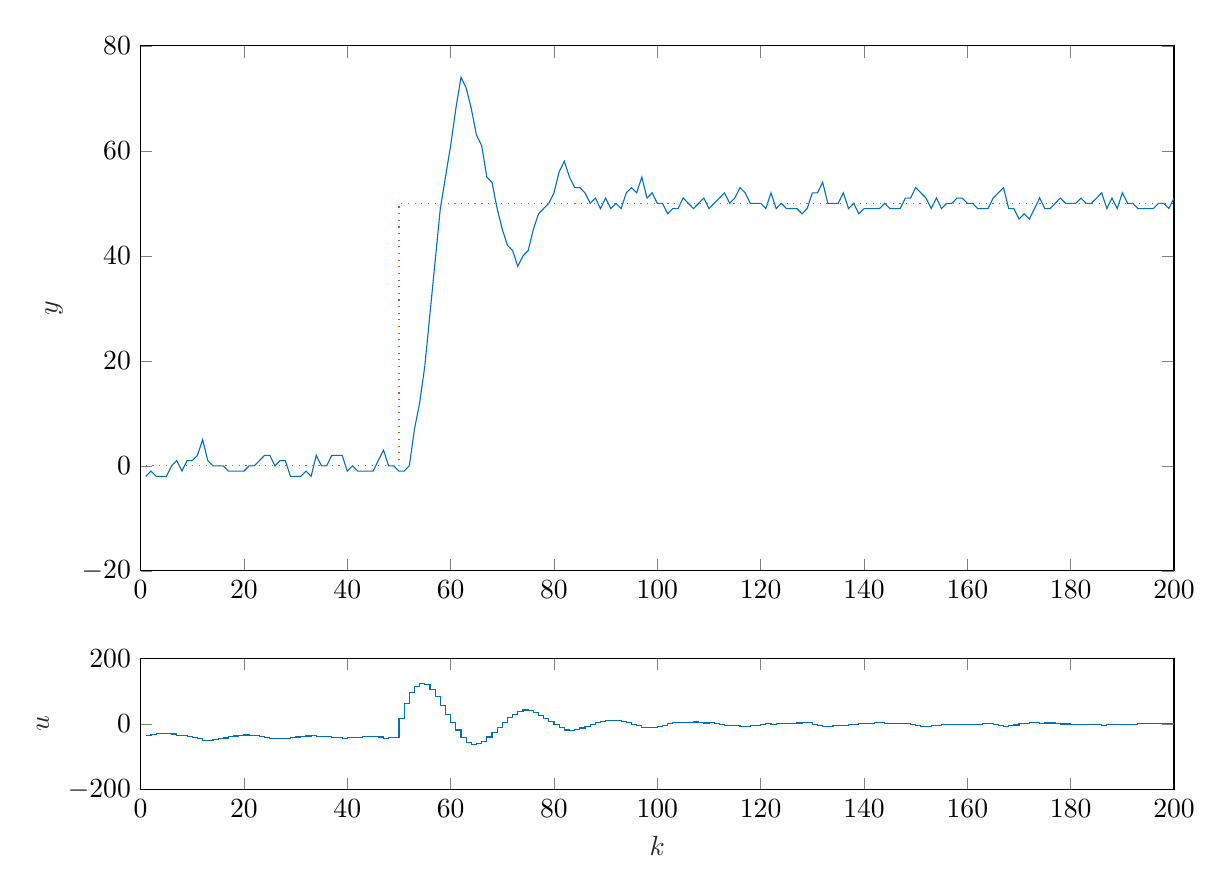
\begin{tikzpicture}

\begin{axis}[%
width=5.167in,
height=0.656in,
at={(0.646in,0.525in)},
scale only axis,
xmin=0,
xmax=200,
xtick={0,20,40,60,80,100,120,140,160,180,200},
xlabel style={font=\color{white!15!black}},
xlabel={$k$},
ymin=-200,
ymax=200,
ytick={-200,0,200},
ylabel style={font=\color{white!15!black}},
ylabel={$u$},
axis background/.style={fill=white}
]
\addplot[const plot, color=mycolor1, forget plot] table[row sep=crcr] {%
1	-34.01\\
2	-31.85\\
3	-29.38\\
4	-28.08\\
5	-27.75\\
6	-30.48\\
7	-34.43\\
8	-35.67\\
9	-39.34\\
10	-42.34\\
11	-45.42\\
12	-50.71\\
13	-49.73\\
14	-47.23\\
15	-44.81\\
16	-42.48\\
17	-39.02\\
18	-36.4\\
19	-34.56\\
20	-33.47\\
21	-34.2\\
22	-35.16\\
23	-37.46\\
24	-40.72\\
25	-43.52\\
26	-43.48\\
27	-44.52\\
28	-45.3\\
29	-42.28\\
30	-39.65\\
31	-37.37\\
32	-36.46\\
33	-34.53\\
34	-37.46\\
35	-37.51\\
36	-37.53\\
37	-39.93\\
38	-41.9\\
39	-43.52\\
40	-41.53\\
41	-41.3\\
42	-40.14\\
43	-39.22\\
44	-38.56\\
45	-37.98\\
46	-39.66\\
47	-43.15\\
48	-42.33\\
49	-41.46\\
50	16.66\\
51	62.17\\
52	96.19\\
53	114.97\\
54	123.43\\
55	120.57\\
56	105.76\\
57	83.07\\
58	55.67\\
59	30.17\\
60	5.94\\
61	-18.31\\
62	-42.03\\
63	-56.54\\
64	-61.8\\
65	-59.11\\
66	-52.89\\
67	-39.48\\
68	-26.78\\
69	-11.27\\
70	4.35\\
71	18.61\\
72	29.15\\
73	39.19\\
74	42.67\\
75	42.07\\
76	35.57\\
77	25.75\\
78	16.16\\
79	7.36\\
80	-0.94\\
81	-10.77\\
82	-18.37\\
83	-19.02\\
84	-15.95\\
85	-12.25\\
86	-7\\
87	-0.21\\
88	4.24\\
89	8.99\\
90	9.49\\
91	11.14\\
92	9.98\\
93	9\\
94	4.25\\
95	-0.99\\
96	-4.05\\
97	-9.56\\
98	-9.25\\
99	-9.55\\
100	-6.95\\
101	-4.27\\
102	0.52\\
103	3.33\\
104	5.48\\
105	4.86\\
106	5.11\\
107	6.1\\
108	5.27\\
109	3.11\\
110	3.37\\
111	2.13\\
112	-0.3\\
113	-3.51\\
114	-3.68\\
115	-4.73\\
116	-7.45\\
117	-8.02\\
118	-5.76\\
119	-3.63\\
120	-1.81\\
121	0.87\\
122	-0.54\\
123	1.51\\
124	1.71\\
125	2.59\\
126	2.93\\
127	3.01\\
128	4.04\\
129	3.54\\
130	-0.28\\
131	-3.24\\
132	-7.71\\
133	-6.56\\
134	-5.36\\
135	-4.21\\
136	-5.18\\
137	-2.39\\
138	-1.42\\
139	1.37\\
140	2.31\\
141	2.85\\
142	3.29\\
143	3.48\\
144	2.38\\
145	2.53\\
146	2.61\\
147	2.61\\
148	0.31\\
149	-1.44\\
150	-4.89\\
151	-6.35\\
152	-6.28\\
153	-3.82\\
154	-3.99\\
155	-1.63\\
156	-0.79\\
157	-0.29\\
158	-1.16\\
159	-2\\
160	-1.66\\
161	-1.44\\
162	-0.24\\
163	0.68\\
164	1.33\\
165	-0.5\\
166	-3.18\\
167	-6.5\\
168	-4.62\\
169	-2.97\\
170	0.7\\
171	2.71\\
172	5.52\\
173	5.41\\
174	2.89\\
175	3.05\\
176	3.01\\
177	1.9\\
178	0.05\\
179	-0.08\\
180	-0.16\\
181	-0.25\\
182	-1.56\\
183	-1.46\\
184	-1.3\\
185	-2.22\\
186	-3.94\\
187	-1.75\\
188	-2.22\\
189	-0.33\\
190	-2.23\\
191	-1.47\\
192	-0.95\\
193	0.47\\
194	1.43\\
195	2.08\\
196	2.57\\
197	1.7\\
198	0.98\\
199	1.46\\
200	-0.34\\
};
\end{axis}

\begin{axis}[%
width=5.167in,
height=2.625in,
at={(0.646in,1.619in)},
scale only axis,
xmin=0,
xmax=200,
xtick={0,20,40,60,80,100,120,140,160,180,200},
ymin=-20,
ymax=80,
ytick={-20,0,20,40,60,80},
ylabel style={font=\color{white!15!black}},
ylabel={$y$},
axis background/.style={fill=white}
]
\addplot [color=mycolor1, forget plot]
  table[row sep=crcr]{%
1	-2\\
2	-1\\
3	-2\\
4	-2\\
5	-2\\
6	0\\
7	1\\
8	-1\\
9	1\\
10	1\\
11	2\\
12	5\\
13	1\\
14	0\\
15	0\\
16	0\\
17	-1\\
18	-1\\
19	-1\\
20	-1\\
21	0\\
22	0\\
23	1\\
24	2\\
25	2\\
26	0\\
27	1\\
28	1\\
29	-2\\
30	-2\\
31	-2\\
32	-1\\
33	-2\\
34	2\\
35	0\\
36	0\\
37	2\\
38	2\\
39	2\\
40	-1\\
41	0\\
42	-1\\
43	-1\\
44	-1\\
45	-1\\
46	1\\
47	3\\
48	0\\
49	0\\
50	-1\\
51	-1\\
52	0\\
53	7\\
54	12\\
55	19\\
56	29\\
57	39\\
58	49\\
59	55\\
60	61\\
61	68\\
62	74\\
63	72\\
64	68\\
65	63\\
66	61\\
67	55\\
68	54\\
69	49\\
70	45\\
71	42\\
72	41\\
73	38\\
74	40\\
75	41\\
76	45\\
77	48\\
78	49\\
79	50\\
80	52\\
81	56\\
82	58\\
83	55\\
84	53\\
85	53\\
86	52\\
87	50\\
88	51\\
89	49\\
90	51\\
91	49\\
92	50\\
93	49\\
94	52\\
95	53\\
96	52\\
97	55\\
98	51\\
99	52\\
100	50\\
101	50\\
102	48\\
103	49\\
104	49\\
105	51\\
106	50\\
107	49\\
108	50\\
109	51\\
110	49\\
111	50\\
112	51\\
113	52\\
114	50\\
115	51\\
116	53\\
117	52\\
118	50\\
119	50\\
120	50\\
121	49\\
122	52\\
123	49\\
124	50\\
125	49\\
126	49\\
127	49\\
128	48\\
129	49\\
130	52\\
131	52\\
132	54\\
133	50\\
134	50\\
135	50\\
136	52\\
137	49\\
138	50\\
139	48\\
140	49\\
141	49\\
142	49\\
143	49\\
144	50\\
145	49\\
146	49\\
147	49\\
148	51\\
149	51\\
150	53\\
151	52\\
152	51\\
153	49\\
154	51\\
155	49\\
156	50\\
157	50\\
158	51\\
159	51\\
160	50\\
161	50\\
162	49\\
163	49\\
164	49\\
165	51\\
166	52\\
167	53\\
168	49\\
169	49\\
170	47\\
171	48\\
172	47\\
173	49\\
174	51\\
175	49\\
176	49\\
177	50\\
178	51\\
179	50\\
180	50\\
181	50\\
182	51\\
183	50\\
184	50\\
185	51\\
186	52\\
187	49\\
188	51\\
189	49\\
190	52\\
191	50\\
192	50\\
193	49\\
194	49\\
195	49\\
196	49\\
197	50\\
198	50\\
199	49\\
200	51\\
};
\addplot[const plot, color=mycolor2, dotted, forget plot] table[row sep=crcr] {%
1	0\\
2	0\\
3	0\\
4	0\\
5	0\\
6	0\\
7	0\\
8	0\\
9	0\\
10	0\\
11	0\\
12	0\\
13	0\\
14	0\\
15	0\\
16	0\\
17	0\\
18	0\\
19	0\\
20	0\\
21	0\\
22	0\\
23	0\\
24	0\\
25	0\\
26	0\\
27	0\\
28	0\\
29	0\\
30	0\\
31	0\\
32	0\\
33	0\\
34	0\\
35	0\\
36	0\\
37	0\\
38	0\\
39	0\\
40	0\\
41	0\\
42	0\\
43	0\\
44	0\\
45	0\\
46	0\\
47	0\\
48	0\\
49	0\\
50	50\\
51	50\\
52	50\\
53	50\\
54	50\\
55	50\\
56	50\\
57	50\\
58	50\\
59	50\\
60	50\\
61	50\\
62	50\\
63	50\\
64	50\\
65	50\\
66	50\\
67	50\\
68	50\\
69	50\\
70	50\\
71	50\\
72	50\\
73	50\\
74	50\\
75	50\\
76	50\\
77	50\\
78	50\\
79	50\\
80	50\\
81	50\\
82	50\\
83	50\\
84	50\\
85	50\\
86	50\\
87	50\\
88	50\\
89	50\\
90	50\\
91	50\\
92	50\\
93	50\\
94	50\\
95	50\\
96	50\\
97	50\\
98	50\\
99	50\\
100	50\\
101	50\\
102	50\\
103	50\\
104	50\\
105	50\\
106	50\\
107	50\\
108	50\\
109	50\\
110	50\\
111	50\\
112	50\\
113	50\\
114	50\\
115	50\\
116	50\\
117	50\\
118	50\\
119	50\\
120	50\\
121	50\\
122	50\\
123	50\\
124	50\\
125	50\\
126	50\\
127	50\\
128	50\\
129	50\\
130	50\\
131	50\\
132	50\\
133	50\\
134	50\\
135	50\\
136	50\\
137	50\\
138	50\\
139	50\\
140	50\\
141	50\\
142	50\\
143	50\\
144	50\\
145	50\\
146	50\\
147	50\\
148	50\\
149	50\\
150	50\\
151	50\\
152	50\\
153	50\\
154	50\\
155	50\\
156	50\\
157	50\\
158	50\\
159	50\\
160	50\\
161	50\\
162	50\\
163	50\\
164	50\\
165	50\\
166	50\\
167	50\\
168	50\\
169	50\\
170	50\\
171	50\\
172	50\\
173	50\\
174	50\\
175	50\\
176	50\\
177	50\\
178	50\\
179	50\\
180	50\\
181	50\\
182	50\\
183	50\\
184	50\\
185	50\\
186	50\\
187	50\\
188	50\\
189	50\\
190	50\\
191	50\\
192	50\\
193	50\\
194	50\\
195	50\\
196	50\\
197	50\\
198	50\\
199	50\\
200	50\\
};
\end{axis}
\end{tikzpicture}%
\end{figure}

\begin{figure}[H]
\centering
%err =15002
\definecolor{mycolor1}{rgb}{0.00000,0.44700,0.74100}%
\definecolor{mycolor2}{rgb}{0.85000,0.32500,0.09800}%
%
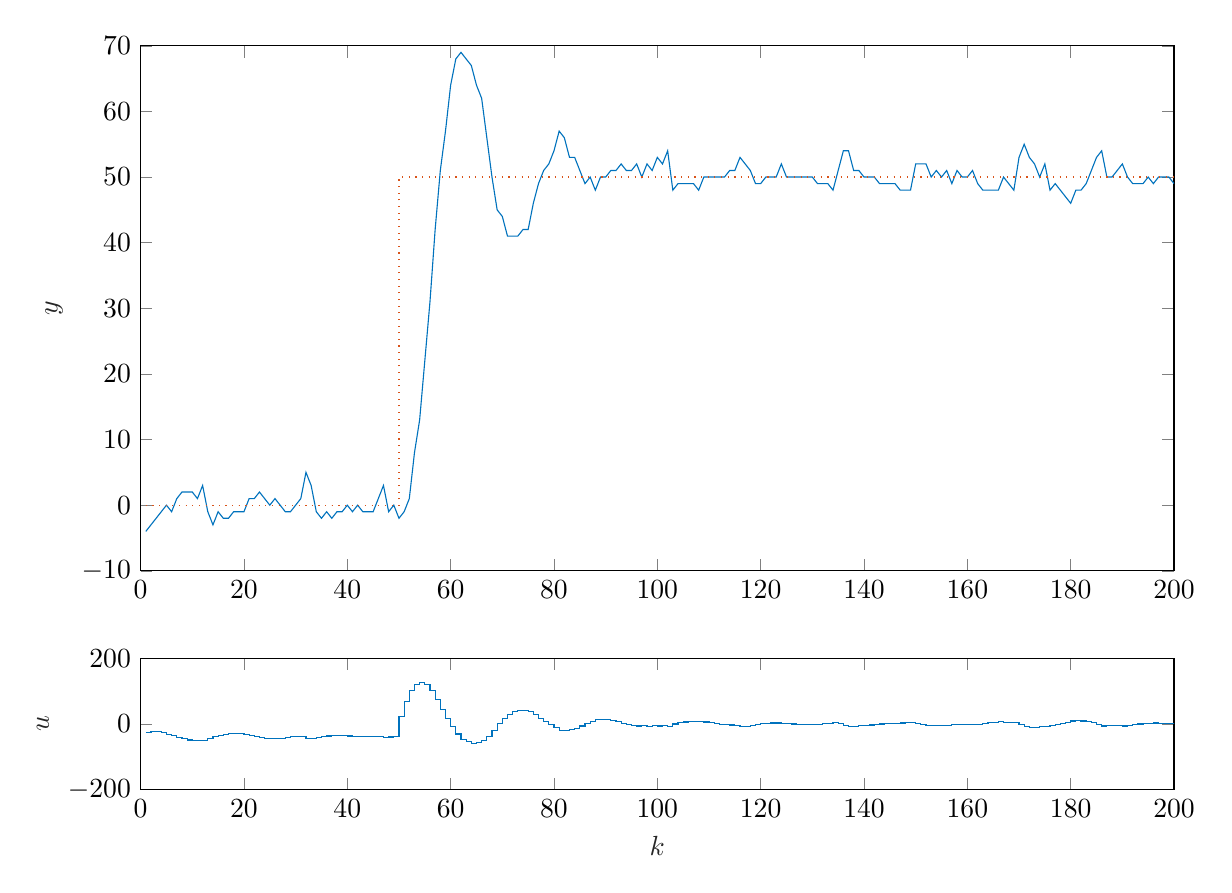
\begin{tikzpicture}

\begin{axis}[%
width=5.167in,
height=0.656in,
at={(0.646in,0.525in)},
scale only axis,
xmin=0,
xmax=200,
xtick={0,20,40,60,80,100,120,140,160,180,200},
xlabel style={font=\color{white!15!black}},
xlabel={$k$},
ymin=-200,
ymax=200,
ytick={-200,0,200},
ylabel style={font=\color{white!15!black}},
ylabel={$u$},
axis background/.style={fill=white}
]
\addplot[const plot, color=mycolor1, forget plot] table[row sep=crcr] {%
1	-24.95\\
2	-22.88\\
3	-23.78\\
4	-27.01\\
5	-31.77\\
6	-35.07\\
7	-40.46\\
8	-45.48\\
9	-48.77\\
10	-50.55\\
11	-49.68\\
12	-50.52\\
13	-45.62\\
14	-38.82\\
15	-35.67\\
16	-32.14\\
17	-29.45\\
18	-29.23\\
19	-29.78\\
20	-30.8\\
21	-34.64\\
22	-37.97\\
23	-41.8\\
24	-43.71\\
25	-43.85\\
26	-44.81\\
27	-43.96\\
28	-41.65\\
29	-39.4\\
30	-38.59\\
31	-38.92\\
32	-43.74\\
33	-45.18\\
34	-41.66\\
35	-37.99\\
36	-36.58\\
37	-34.42\\
38	-34.25\\
39	-34.69\\
40	-36.65\\
41	-37.18\\
42	-38.74\\
43	-38.47\\
44	-37.89\\
45	-37.08\\
46	-38.46\\
47	-41.8\\
48	-39.63\\
49	-39.17\\
50	22.93\\
51	69.83\\
52	103.11\\
53	120.42\\
54	126.99\\
55	119.38\\
56	101.17\\
57	74.24\\
58	44.45\\
59	17.42\\
60	-8.68\\
61	-30.51\\
62	-46.1\\
63	-54.76\\
64	-58.44\\
65	-56.32\\
66	-50.27\\
67	-36.93\\
68	-18.8\\
69	0.83\\
70	15.74\\
71	29.11\\
72	37.12\\
73	40.89\\
74	39.92\\
75	36.86\\
76	28.29\\
77	17.3\\
78	6.43\\
79	-2.58\\
80	-10.53\\
81	-18.72\\
82	-21.21\\
83	-17.5\\
84	-13.24\\
85	-6.27\\
86	2.4\\
87	7.59\\
88	13.69\\
89	14.45\\
90	13.61\\
91	10.65\\
92	6.93\\
93	1.79\\
94	-1.2\\
95	-3.52\\
96	-6.31\\
97	-5.31\\
98	-6.45\\
99	-5.38\\
100	-6.24\\
101	-5.17\\
102	-6.42\\
103	-0.11\\
104	3.51\\
105	5.96\\
106	7.42\\
107	7.87\\
108	8.55\\
109	5.92\\
110	3.33\\
111	1.13\\
112	-0.52\\
113	-1.61\\
114	-3.25\\
115	-3.98\\
116	-6.48\\
117	-6.84\\
118	-5.58\\
119	-2.01\\
120	0.99\\
121	2.14\\
122	2.86\\
123	3.07\\
124	0.43\\
125	0.21\\
126	-0.13\\
127	-0.6\\
128	-1.06\\
129	-1.25\\
130	-1.4\\
131	-0.31\\
132	0.58\\
133	1.34\\
134	3.23\\
135	1.41\\
136	-3.49\\
137	-7.2\\
138	-6.5\\
139	-5.98\\
140	-4.43\\
141	-3.03\\
142	-2.01\\
143	-0.2\\
144	0.94\\
145	1.48\\
146	1.75\\
147	3.14\\
148	4.27\\
149	5.21\\
150	1.29\\
151	-1.69\\
152	-4\\
153	-3.54\\
154	-4.34\\
155	-3.54\\
156	-3.89\\
157	-1.68\\
158	-2.38\\
159	-1.9\\
160	-1.52\\
161	-2.44\\
162	-0.8\\
163	1.73\\
164	3.7\\
165	5.15\\
166	6.23\\
167	4.43\\
168	3.94\\
169	4.67\\
170	-0.68\\
171	-7.09\\
172	-9.41\\
173	-9.84\\
174	-7.65\\
175	-8.02\\
176	-3.29\\
177	-0.76\\
178	2.28\\
179	5.62\\
180	9.15\\
181	9.3\\
182	9.19\\
183	7.79\\
184	4.16\\
185	-0.98\\
186	-6.2\\
187	-5.39\\
188	-4.69\\
189	-5.08\\
190	-6.23\\
191	-4.5\\
192	-1.89\\
193	0.05\\
194	1.55\\
195	1.71\\
196	3.03\\
197	2.78\\
198	2.42\\
199	1.92\\
200	2.57\\
};
\end{axis}

\begin{axis}[%
width=5.167in,
height=2.625in,
at={(0.646in,1.619in)},
scale only axis,
xmin=0,
xmax=200,
xtick={0,20,40,60,80,100,120,140,160,180,200},
ymin=-10,
ymax=70,
ytick={-10,0,10,20,30,40,50,60,70},
ylabel style={font=\color{white!15!black}},
ylabel={$y$},
axis background/.style={fill=white}
]
\addplot [color=mycolor1, forget plot]
  table[row sep=crcr]{%
1	-4\\
2	-3\\
3	-2\\
4	-1\\
5	0\\
6	-1\\
7	1\\
8	2\\
9	2\\
10	2\\
11	1\\
12	3\\
13	-1\\
14	-3\\
15	-1\\
16	-2\\
17	-2\\
18	-1\\
19	-1\\
20	-1\\
21	1\\
22	1\\
23	2\\
24	1\\
25	0\\
26	1\\
27	0\\
28	-1\\
29	-1\\
30	0\\
31	1\\
32	5\\
33	3\\
34	-1\\
35	-2\\
36	-1\\
37	-2\\
38	-1\\
39	-1\\
40	0\\
41	-1\\
42	0\\
43	-1\\
44	-1\\
45	-1\\
46	1\\
47	3\\
48	-1\\
49	0\\
50	-2\\
51	-1\\
52	1\\
53	8\\
54	13\\
55	22\\
56	31\\
57	42\\
58	51\\
59	57\\
60	64\\
61	68\\
62	69\\
63	68\\
64	67\\
65	64\\
66	62\\
67	56\\
68	50\\
69	45\\
70	44\\
71	41\\
72	41\\
73	41\\
74	42\\
75	42\\
76	46\\
77	49\\
78	51\\
79	52\\
80	54\\
81	57\\
82	56\\
83	53\\
84	53\\
85	51\\
86	49\\
87	50\\
88	48\\
89	50\\
90	50\\
91	51\\
92	51\\
93	52\\
94	51\\
95	51\\
96	52\\
97	50\\
98	52\\
99	51\\
100	53\\
101	52\\
102	54\\
103	48\\
104	49\\
105	49\\
106	49\\
107	49\\
108	48\\
109	50\\
110	50\\
111	50\\
112	50\\
113	50\\
114	51\\
115	51\\
116	53\\
117	52\\
118	51\\
119	49\\
120	49\\
121	50\\
122	50\\
123	50\\
124	52\\
125	50\\
126	50\\
127	50\\
128	50\\
129	50\\
130	50\\
131	49\\
132	49\\
133	49\\
134	48\\
135	51\\
136	54\\
137	54\\
138	51\\
139	51\\
140	50\\
141	50\\
142	50\\
143	49\\
144	49\\
145	49\\
146	49\\
147	48\\
148	48\\
149	48\\
150	52\\
151	52\\
152	52\\
153	50\\
154	51\\
155	50\\
156	51\\
157	49\\
158	51\\
159	50\\
160	50\\
161	51\\
162	49\\
163	48\\
164	48\\
165	48\\
166	48\\
167	50\\
168	49\\
169	48\\
170	53\\
171	55\\
172	53\\
173	52\\
174	50\\
175	52\\
176	48\\
177	49\\
178	48\\
179	47\\
180	46\\
181	48\\
182	48\\
183	49\\
184	51\\
185	53\\
186	54\\
187	50\\
188	50\\
189	51\\
190	52\\
191	50\\
192	49\\
193	49\\
194	49\\
195	50\\
196	49\\
197	50\\
198	50\\
199	50\\
200	49\\
};
\addplot[const plot, color=mycolor2, dotted, forget plot] table[row sep=crcr] {%
1	0\\
2	0\\
3	0\\
4	0\\
5	0\\
6	0\\
7	0\\
8	0\\
9	0\\
10	0\\
11	0\\
12	0\\
13	0\\
14	0\\
15	0\\
16	0\\
17	0\\
18	0\\
19	0\\
20	0\\
21	0\\
22	0\\
23	0\\
24	0\\
25	0\\
26	0\\
27	0\\
28	0\\
29	0\\
30	0\\
31	0\\
32	0\\
33	0\\
34	0\\
35	0\\
36	0\\
37	0\\
38	0\\
39	0\\
40	0\\
41	0\\
42	0\\
43	0\\
44	0\\
45	0\\
46	0\\
47	0\\
48	0\\
49	0\\
50	50\\
51	50\\
52	50\\
53	50\\
54	50\\
55	50\\
56	50\\
57	50\\
58	50\\
59	50\\
60	50\\
61	50\\
62	50\\
63	50\\
64	50\\
65	50\\
66	50\\
67	50\\
68	50\\
69	50\\
70	50\\
71	50\\
72	50\\
73	50\\
74	50\\
75	50\\
76	50\\
77	50\\
78	50\\
79	50\\
80	50\\
81	50\\
82	50\\
83	50\\
84	50\\
85	50\\
86	50\\
87	50\\
88	50\\
89	50\\
90	50\\
91	50\\
92	50\\
93	50\\
94	50\\
95	50\\
96	50\\
97	50\\
98	50\\
99	50\\
100	50\\
101	50\\
102	50\\
103	50\\
104	50\\
105	50\\
106	50\\
107	50\\
108	50\\
109	50\\
110	50\\
111	50\\
112	50\\
113	50\\
114	50\\
115	50\\
116	50\\
117	50\\
118	50\\
119	50\\
120	50\\
121	50\\
122	50\\
123	50\\
124	50\\
125	50\\
126	50\\
127	50\\
128	50\\
129	50\\
130	50\\
131	50\\
132	50\\
133	50\\
134	50\\
135	50\\
136	50\\
137	50\\
138	50\\
139	50\\
140	50\\
141	50\\
142	50\\
143	50\\
144	50\\
145	50\\
146	50\\
147	50\\
148	50\\
149	50\\
150	50\\
151	50\\
152	50\\
153	50\\
154	50\\
155	50\\
156	50\\
157	50\\
158	50\\
159	50\\
160	50\\
161	50\\
162	50\\
163	50\\
164	50\\
165	50\\
166	50\\
167	50\\
168	50\\
169	50\\
170	50\\
171	50\\
172	50\\
173	50\\
174	50\\
175	50\\
176	50\\
177	50\\
178	50\\
179	50\\
180	50\\
181	50\\
182	50\\
183	50\\
184	50\\
185	50\\
186	50\\
187	50\\
188	50\\
189	50\\
190	50\\
191	50\\
192	50\\
193	50\\
194	50\\
195	50\\
196	50\\
197	50\\
198	50\\
199	50\\
200	50\\
};
\end{axis}
\end{tikzpicture}%
\end{figure}

\begin{figure}[H]
\centering
%err =15137
\definecolor{mycolor1}{rgb}{0.00000,0.44700,0.74100}%
\definecolor{mycolor2}{rgb}{0.85000,0.32500,0.09800}%
%
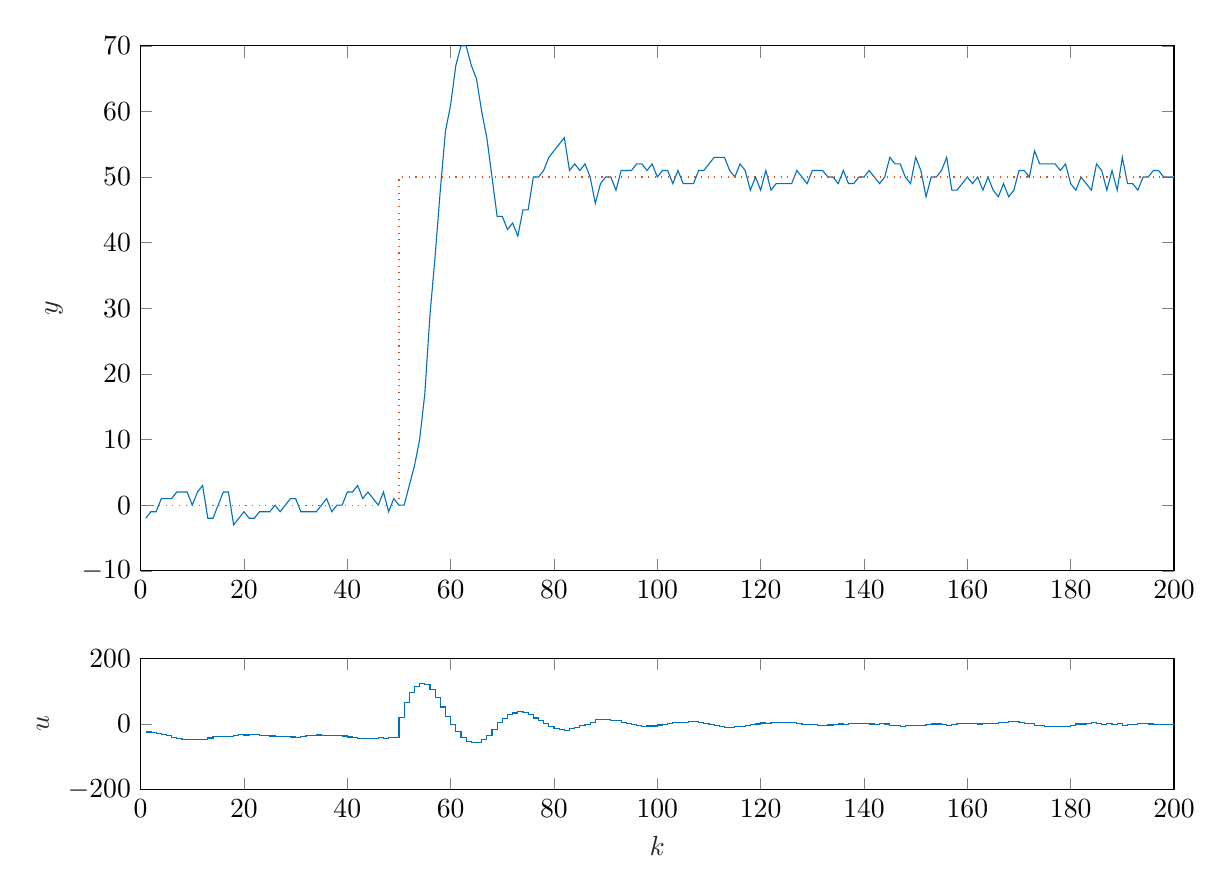
\begin{tikzpicture}

\begin{axis}[%
width=5.167in,
height=0.656in,
at={(0.646in,0.525in)},
scale only axis,
xmin=0,
xmax=200,
xtick={0,20,40,60,80,100,120,140,160,180,200},
xlabel style={font=\color{white!15!black}},
xlabel={$k$},
ymin=-200,
ymax=200,
ytick={-200,0,200},
ylabel style={font=\color{white!15!black}},
ylabel={$u$},
axis background/.style={fill=white}
]
\addplot[const plot, color=mycolor1, forget plot] table[row sep=crcr] {%
1	-24.55\\
2	-25.86\\
3	-27.68\\
4	-32.24\\
5	-36.46\\
6	-39.97\\
7	-43.97\\
8	-46.76\\
9	-48.53\\
10	-47.03\\
11	-47.53\\
12	-48.48\\
13	-42.83\\
14	-38.16\\
15	-36.89\\
16	-38.23\\
17	-39.32\\
18	-34.79\\
19	-33.14\\
20	-33.6\\
21	-33.05\\
22	-32.99\\
23	-34.36\\
24	-35.68\\
25	-36.69\\
26	-38.35\\
27	-37.99\\
28	-38.54\\
29	-39.64\\
30	-40.05\\
31	-37.72\\
32	-35.81\\
33	-34.47\\
34	-33.53\\
35	-34.02\\
36	-35.78\\
37	-35.08\\
38	-35.89\\
39	-36.68\\
40	-39.59\\
41	-41.66\\
42	-44.37\\
43	-44.01\\
44	-44.78\\
45	-44.02\\
46	-42.08\\
47	-42.93\\
48	-40.04\\
49	-40.31\\
50	19.72\\
51	65.28\\
52	95.52\\
53	115\\
54	124.5\\
55	121.67\\
56	103.95\\
57	80.06\\
58	51.7\\
59	22.5\\
60	-1.56\\
61	-23.91\\
62	-41.88\\
63	-53.31\\
64	-56.52\\
65	-55.33\\
66	-46.78\\
67	-34.09\\
68	-16.74\\
69	3.31\\
70	17.14\\
71	28.39\\
72	33.63\\
73	37.89\\
74	34.01\\
75	29\\
76	18.17\\
77	9.26\\
78	1.28\\
79	-6.75\\
80	-12.85\\
81	-17.4\\
82	-19.79\\
83	-14\\
84	-9.68\\
85	-4.19\\
86	-0.36\\
87	4.66\\
88	12.89\\
89	14.18\\
90	12.77\\
91	10.8\\
92	10.39\\
93	5.4\\
94	1.36\\
95	-1.64\\
96	-4.81\\
97	-6.51\\
98	-6.02\\
99	-6.03\\
100	-3\\
101	-1.25\\
102	0.2\\
103	3.61\\
104	3.74\\
105	5.81\\
106	6.89\\
107	7.13\\
108	4.31\\
109	1.78\\
110	-1.69\\
111	-5.69\\
112	-8.83\\
113	-10.92\\
114	-9.81\\
115	-7.28\\
116	-7.34\\
117	-5.96\\
118	-1.17\\
119	0.03\\
120	3.15\\
121	1.86\\
122	4.09\\
123	4.38\\
124	4.29\\
125	3.83\\
126	3.31\\
127	0.36\\
128	-0.78\\
129	-0.39\\
130	-2.35\\
131	-3.61\\
132	-4.16\\
133	-3.15\\
134	-2.24\\
135	-0.12\\
136	-0.74\\
137	1.11\\
138	2.5\\
139	2.15\\
140	1.65\\
141	0.03\\
142	-0.24\\
143	0.62\\
144	0.01\\
145	-3.99\\
146	-5.75\\
147	-6.98\\
148	-5.61\\
149	-3.28\\
150	-5.97\\
151	-5.52\\
152	-0.32\\
153	-0.13\\
154	-0.16\\
155	-1.35\\
156	-4.74\\
157	-1.68\\
158	0.62\\
159	1\\
160	0.24\\
161	0.89\\
162	-0\\
163	1.51\\
164	0.3\\
165	1.89\\
166	4.48\\
167	4.18\\
168	6.37\\
169	7.03\\
170	3.99\\
171	1.59\\
172	0.94\\
173	-4.25\\
174	-5.71\\
175	-6.48\\
176	-7.03\\
177	-7.44\\
178	-6.46\\
179	-6.89\\
180	-3.73\\
181	-0.17\\
182	0\\
183	1.22\\
184	3.44\\
185	0.13\\
186	-1.46\\
187	0.86\\
188	-1.13\\
189	0.91\\
190	-3.33\\
191	-1.97\\
192	-0.85\\
193	1.14\\
194	0.23\\
195	-0.2\\
196	-1.63\\
197	-2.66\\
198	-2.07\\
199	-1.67\\
200	-1.26\\
};
\end{axis}

\begin{axis}[%
width=5.167in,
height=2.625in,
at={(0.646in,1.619in)},
scale only axis,
xmin=0,
xmax=200,
xtick={0,20,40,60,80,100,120,140,160,180,200},
ymin=-10,
ymax=70,
ytick={-10,0,10,20,30,40,50,60,70},
ylabel style={font=\color{white!15!black}},
ylabel={$y$},
axis background/.style={fill=white}
]
\addplot [color=mycolor1, forget plot]
  table[row sep=crcr]{%
1	-2\\
2	-1\\
3	-1\\
4	1\\
5	1\\
6	1\\
7	2\\
8	2\\
9	2\\
10	0\\
11	2\\
12	3\\
13	-2\\
14	-2\\
15	0\\
16	2\\
17	2\\
18	-3\\
19	-2\\
20	-1\\
21	-2\\
22	-2\\
23	-1\\
24	-1\\
25	-1\\
26	0\\
27	-1\\
28	0\\
29	1\\
30	1\\
31	-1\\
32	-1\\
33	-1\\
34	-1\\
35	0\\
36	1\\
37	-1\\
38	0\\
39	0\\
40	2\\
41	2\\
42	3\\
43	1\\
44	2\\
45	1\\
46	0\\
47	2\\
48	-1\\
49	1\\
50	0\\
51	0\\
52	3\\
53	6\\
54	10\\
55	17\\
56	29\\
57	38\\
58	48\\
59	57\\
60	61\\
61	67\\
62	70\\
63	70\\
64	67\\
65	65\\
66	60\\
67	56\\
68	50\\
69	44\\
70	44\\
71	42\\
72	43\\
73	41\\
74	45\\
75	45\\
76	50\\
77	50\\
78	51\\
79	53\\
80	54\\
81	55\\
82	56\\
83	51\\
84	52\\
85	51\\
86	52\\
87	50\\
88	46\\
89	49\\
90	50\\
91	50\\
92	48\\
93	51\\
94	51\\
95	51\\
96	52\\
97	52\\
98	51\\
99	52\\
100	50\\
101	51\\
102	51\\
103	49\\
104	51\\
105	49\\
106	49\\
107	49\\
108	51\\
109	51\\
110	52\\
111	53\\
112	53\\
113	53\\
114	51\\
115	50\\
116	52\\
117	51\\
118	48\\
119	50\\
120	48\\
121	51\\
122	48\\
123	49\\
124	49\\
125	49\\
126	49\\
127	51\\
128	50\\
129	49\\
130	51\\
131	51\\
132	51\\
133	50\\
134	50\\
135	49\\
136	51\\
137	49\\
138	49\\
139	50\\
140	50\\
141	51\\
142	50\\
143	49\\
144	50\\
145	53\\
146	52\\
147	52\\
148	50\\
149	49\\
150	53\\
151	51\\
152	47\\
153	50\\
154	50\\
155	51\\
156	53\\
157	48\\
158	48\\
159	49\\
160	50\\
161	49\\
162	50\\
163	48\\
164	50\\
165	48\\
166	47\\
167	49\\
168	47\\
169	48\\
170	51\\
171	51\\
172	50\\
173	54\\
174	52\\
175	52\\
176	52\\
177	52\\
178	51\\
179	52\\
180	49\\
181	48\\
182	50\\
183	49\\
184	48\\
185	52\\
186	51\\
187	48\\
188	51\\
189	48\\
190	53\\
191	49\\
192	49\\
193	48\\
194	50\\
195	50\\
196	51\\
197	51\\
198	50\\
199	50\\
200	50\\
};
\addplot[const plot, color=mycolor2, dotted, forget plot] table[row sep=crcr] {%
1	0\\
2	0\\
3	0\\
4	0\\
5	0\\
6	0\\
7	0\\
8	0\\
9	0\\
10	0\\
11	0\\
12	0\\
13	0\\
14	0\\
15	0\\
16	0\\
17	0\\
18	0\\
19	0\\
20	0\\
21	0\\
22	0\\
23	0\\
24	0\\
25	0\\
26	0\\
27	0\\
28	0\\
29	0\\
30	0\\
31	0\\
32	0\\
33	0\\
34	0\\
35	0\\
36	0\\
37	0\\
38	0\\
39	0\\
40	0\\
41	0\\
42	0\\
43	0\\
44	0\\
45	0\\
46	0\\
47	0\\
48	0\\
49	0\\
50	50\\
51	50\\
52	50\\
53	50\\
54	50\\
55	50\\
56	50\\
57	50\\
58	50\\
59	50\\
60	50\\
61	50\\
62	50\\
63	50\\
64	50\\
65	50\\
66	50\\
67	50\\
68	50\\
69	50\\
70	50\\
71	50\\
72	50\\
73	50\\
74	50\\
75	50\\
76	50\\
77	50\\
78	50\\
79	50\\
80	50\\
81	50\\
82	50\\
83	50\\
84	50\\
85	50\\
86	50\\
87	50\\
88	50\\
89	50\\
90	50\\
91	50\\
92	50\\
93	50\\
94	50\\
95	50\\
96	50\\
97	50\\
98	50\\
99	50\\
100	50\\
101	50\\
102	50\\
103	50\\
104	50\\
105	50\\
106	50\\
107	50\\
108	50\\
109	50\\
110	50\\
111	50\\
112	50\\
113	50\\
114	50\\
115	50\\
116	50\\
117	50\\
118	50\\
119	50\\
120	50\\
121	50\\
122	50\\
123	50\\
124	50\\
125	50\\
126	50\\
127	50\\
128	50\\
129	50\\
130	50\\
131	50\\
132	50\\
133	50\\
134	50\\
135	50\\
136	50\\
137	50\\
138	50\\
139	50\\
140	50\\
141	50\\
142	50\\
143	50\\
144	50\\
145	50\\
146	50\\
147	50\\
148	50\\
149	50\\
150	50\\
151	50\\
152	50\\
153	50\\
154	50\\
155	50\\
156	50\\
157	50\\
158	50\\
159	50\\
160	50\\
161	50\\
162	50\\
163	50\\
164	50\\
165	50\\
166	50\\
167	50\\
168	50\\
169	50\\
170	50\\
171	50\\
172	50\\
173	50\\
174	50\\
175	50\\
176	50\\
177	50\\
178	50\\
179	50\\
180	50\\
181	50\\
182	50\\
183	50\\
184	50\\
185	50\\
186	50\\
187	50\\
188	50\\
189	50\\
190	50\\
191	50\\
192	50\\
193	50\\
194	50\\
195	50\\
196	50\\
197	50\\
198	50\\
199	50\\
200	50\\
};
\end{axis}
\end{tikzpicture}%
\end{figure}


\begin{figure}[H]
\centering
%err =226975
\definecolor{mycolor1}{rgb}{0.00000,0.44700,0.74100}%
\definecolor{mycolor2}{rgb}{0.85000,0.32500,0.09800}%
%
\begin{tikzpicture}

\begin{axis}[%
width=5.167in,
height=0.656in,
at={(0.646in,0.525in)},
scale only axis,
xmin=0,
xmax=200,
xtick={0,20,40,60,80,100,120,140,160,180,200},
xlabel style={font=\color{white!15!black}},
xlabel={$k$},
ymin=-500,
ymax=500,
ytick={-500,0,500},
ylabel style={font=\color{white!15!black}},
ylabel={$u$},
axis background/.style={fill=white}
]
\addplot[const plot, color=mycolor1, forget plot] table[row sep=crcr] {%
1	-31.28\\
2	-34.33\\
3	-35.97\\
4	-35.46\\
5	-35.83\\
6	-36.86\\
7	-39.27\\
8	-40.15\\
9	-39.89\\
10	-40.46\\
11	-39.84\\
12	-40.85\\
13	-38.99\\
14	-39.11\\
15	-38.43\\
16	-39.71\\
17	-39.12\\
18	-37.89\\
19	-37.97\\
20	-37.25\\
21	-37.58\\
22	-37.94\\
23	-35.76\\
24	-38.25\\
25	-44.49\\
26	-43.42\\
27	-44.08\\
28	-44.64\\
29	-40.69\\
30	-39.09\\
31	-37.88\\
32	-36.11\\
33	-35.68\\
34	-35.6\\
35	-34.75\\
36	-34.08\\
37	-33.6\\
38	-35.74\\
39	-37.38\\
40	-37.83\\
41	-38.22\\
42	-40.19\\
43	-39.97\\
44	-40.51\\
45	-39.11\\
46	-39.63\\
47	-37.48\\
48	-36.59\\
49	-35.86\\
50	134.15\\
51	267.8\\
52	367.24\\
53	432.47\\
54	469.98\\
55	474.24\\
56	453.69\\
57	419.01\\
58	376.23\\
59	325.2\\
60	267.22\\
61	212.47\\
62	161.5\\
63	118.33\\
64	89.96\\
65	67.63\\
66	56.64\\
67	53.38\\
68	59.58\\
69	71.28\\
70	83.52\\
71	97.78\\
72	111.7\\
73	126.89\\
74	138.26\\
75	147.22\\
76	150.74\\
77	154.44\\
78	157.44\\
79	158.41\\
80	158.27\\
81	158.47\\
82	160.41\\
83	162.98\\
84	164.58\\
85	165.16\\
86	168.07\\
87	170.89\\
88	170.82\\
89	167.35\\
90	163.47\\
91	160.25\\
92	156.6\\
93	148.03\\
94	141.77\\
95	137.07\\
96	137.99\\
97	137.15\\
98	136.85\\
99	138.95\\
100	143.44\\
101	147.84\\
102	150.28\\
103	151.88\\
104	153.58\\
105	154.38\\
106	154.31\\
107	152.8\\
108	151.09\\
109	150.16\\
110	149.07\\
111	147.98\\
112	147.92\\
113	144.65\\
114	144.75\\
115	145.12\\
116	146.48\\
117	147.03\\
118	148.64\\
119	150.11\\
120	150.43\\
121	151.45\\
122	150.48\\
123	150.41\\
124	151.92\\
125	151.24\\
126	150.59\\
127	152.61\\
128	148.31\\
129	143.96\\
130	143.13\\
131	144.25\\
132	142.77\\
133	143.46\\
134	145.04\\
135	147.99\\
136	147.7\\
137	149.04\\
138	151.65\\
139	151.84\\
140	151.87\\
141	151.85\\
142	151.75\\
143	150.76\\
144	150.81\\
145	147.4\\
146	146.42\\
147	145.78\\
148	144.49\\
149	145.25\\
150	145.17\\
151	146.86\\
152	148.27\\
153	150.27\\
154	150.96\\
155	151.46\\
156	150.99\\
157	149.65\\
158	146.79\\
159	144.51\\
160	143.49\\
161	145.19\\
162	144.04\\
163	144.01\\
164	142.3\\
165	145.19\\
166	143.17\\
167	144.11\\
168	146.64\\
169	147.81\\
170	148.76\\
171	147.82\\
172	147.8\\
173	145.1\\
174	145.37\\
175	146.33\\
176	147.08\\
177	146.82\\
178	146.67\\
179	146.57\\
180	146.37\\
181	147.08\\
182	146.86\\
183	147.6\\
184	150.03\\
185	150.32\\
186	150.54\\
187	150.72\\
188	152.5\\
189	150.42\\
190	147.02\\
191	145.24\\
192	143.83\\
193	143.62\\
194	144.33\\
195	144.16\\
196	145.77\\
197	145.46\\
198	146.82\\
199	146.18\\
200	149.04\\
};
\end{axis}

\begin{axis}[%
width=5.167in,
height=2.625in,
at={(0.646in,1.619in)},
scale only axis,
xmin=0,
xmax=200,
xtick={0,20,40,60,80,100,120,140,160,180,200},
ymin=-50,
ymax=250,
ytick={-50,0,50,100,150,200,250},
ylabel style={font=\color{white!15!black}},
ylabel={$y$},
axis background/.style={fill=white}
]
\addplot [color=mycolor1, forget plot]
  table[row sep=crcr]{%
1	-2\\
2	1\\
3	0\\
4	-2\\
5	-1\\
6	0\\
7	2\\
8	1\\
9	0\\
10	1\\
11	0\\
12	2\\
13	-1\\
14	1\\
15	0\\
16	2\\
17	0\\
18	-1\\
19	0\\
20	-1\\
21	0\\
22	0\\
23	-3\\
24	2\\
25	7\\
26	0\\
27	2\\
28	2\\
29	-3\\
30	-1\\
31	-1\\
32	-2\\
33	-1\\
34	-1\\
35	-2\\
36	-2\\
37	-2\\
38	1\\
39	1\\
40	0\\
41	0\\
42	2\\
43	0\\
44	1\\
45	-1\\
46	1\\
47	-2\\
48	-1\\
49	-1\\
50	-1\\
51	1\\
52	8\\
53	25\\
54	41\\
55	68\\
56	94\\
57	117\\
58	140\\
59	168\\
60	196\\
61	214\\
62	229\\
63	238\\
64	237\\
65	242\\
66	241\\
67	241\\
68	235\\
69	229\\
70	225\\
71	218\\
72	212\\
73	204\\
74	200\\
75	195\\
76	195\\
77	190\\
78	187\\
79	187\\
80	188\\
81	188\\
82	189\\
83	190\\
84	192\\
85	195\\
86	194\\
87	194\\
88	198\\
89	201\\
90	202\\
91	202\\
92	202\\
93	208\\
94	208\\
95	208\\
96	203\\
97	206\\
98	206\\
99	204\\
100	201\\
101	200\\
102	201\\
103	201\\
104	200\\
105	200\\
106	200\\
107	201\\
108	201\\
109	200\\
110	200\\
111	200\\
112	199\\
113	203\\
114	200\\
115	200\\
116	199\\
117	200\\
118	199\\
119	199\\
120	200\\
121	199\\
122	201\\
123	200\\
124	198\\
125	200\\
126	200\\
127	197\\
128	204\\
129	205\\
130	202\\
131	200\\
132	203\\
133	201\\
134	200\\
135	198\\
136	201\\
137	199\\
138	197\\
139	199\\
140	199\\
141	199\\
142	199\\
143	200\\
144	199\\
145	203\\
146	201\\
147	201\\
148	202\\
149	200\\
150	201\\
151	199\\
152	199\\
153	198\\
154	199\\
155	199\\
156	200\\
157	201\\
158	203\\
159	203\\
160	202\\
161	199\\
162	202\\
163	201\\
164	203\\
165	198\\
166	203\\
167	200\\
168	198\\
169	199\\
170	199\\
171	201\\
172	200\\
173	203\\
174	200\\
175	199\\
176	199\\
177	200\\
178	200\\
179	200\\
180	200\\
181	199\\
182	200\\
183	199\\
184	197\\
185	199\\
186	199\\
187	199\\
188	197\\
189	201\\
190	203\\
191	202\\
192	202\\
193	201\\
194	200\\
195	201\\
196	199\\
197	201\\
198	199\\
199	201\\
200	197\\
};
\addplot[const plot, color=mycolor2, dotted, forget plot] table[row sep=crcr] {%
1	0\\
2	0\\
3	0\\
4	0\\
5	0\\
6	0\\
7	0\\
8	0\\
9	0\\
10	0\\
11	0\\
12	0\\
13	0\\
14	0\\
15	0\\
16	0\\
17	0\\
18	0\\
19	0\\
20	0\\
21	0\\
22	0\\
23	0\\
24	0\\
25	0\\
26	0\\
27	0\\
28	0\\
29	0\\
30	0\\
31	0\\
32	0\\
33	0\\
34	0\\
35	0\\
36	0\\
37	0\\
38	0\\
39	0\\
40	0\\
41	0\\
42	0\\
43	0\\
44	0\\
45	0\\
46	0\\
47	0\\
48	0\\
49	0\\
50	200\\
51	200\\
52	200\\
53	200\\
54	200\\
55	200\\
56	200\\
57	200\\
58	200\\
59	200\\
60	200\\
61	200\\
62	200\\
63	200\\
64	200\\
65	200\\
66	200\\
67	200\\
68	200\\
69	200\\
70	200\\
71	200\\
72	200\\
73	200\\
74	200\\
75	200\\
76	200\\
77	200\\
78	200\\
79	200\\
80	200\\
81	200\\
82	200\\
83	200\\
84	200\\
85	200\\
86	200\\
87	200\\
88	200\\
89	200\\
90	200\\
91	200\\
92	200\\
93	200\\
94	200\\
95	200\\
96	200\\
97	200\\
98	200\\
99	200\\
100	200\\
101	200\\
102	200\\
103	200\\
104	200\\
105	200\\
106	200\\
107	200\\
108	200\\
109	200\\
110	200\\
111	200\\
112	200\\
113	200\\
114	200\\
115	200\\
116	200\\
117	200\\
118	200\\
119	200\\
120	200\\
121	200\\
122	200\\
123	200\\
124	200\\
125	200\\
126	200\\
127	200\\
128	200\\
129	200\\
130	200\\
131	200\\
132	200\\
133	200\\
134	200\\
135	200\\
136	200\\
137	200\\
138	200\\
139	200\\
140	200\\
141	200\\
142	200\\
143	200\\
144	200\\
145	200\\
146	200\\
147	200\\
148	200\\
149	200\\
150	200\\
151	200\\
152	200\\
153	200\\
154	200\\
155	200\\
156	200\\
157	200\\
158	200\\
159	200\\
160	200\\
161	200\\
162	200\\
163	200\\
164	200\\
165	200\\
166	200\\
167	200\\
168	200\\
169	200\\
170	200\\
171	200\\
172	200\\
173	200\\
174	200\\
175	200\\
176	200\\
177	200\\
178	200\\
179	200\\
180	200\\
181	200\\
182	200\\
183	200\\
184	200\\
185	200\\
186	200\\
187	200\\
188	200\\
189	200\\
190	200\\
191	200\\
192	200\\
193	200\\
194	200\\
195	200\\
196	200\\
197	200\\
198	200\\
199	200\\
200	200\\
};
\end{axis}
\end{tikzpicture}%
\end{figure}

\begin{figure}[H]
\centering
%err =215448
\definecolor{mycolor1}{rgb}{0.00000,0.44700,0.74100}%
\definecolor{mycolor2}{rgb}{0.85000,0.32500,0.09800}%
%
\begin{tikzpicture}

\begin{axis}[%
width=5.167in,
height=0.656in,
at={(0.646in,0.525in)},
scale only axis,
xmin=0,
xmax=200,
xtick={0,20,40,60,80,100,120,140,160,180,200},
xlabel style={font=\color{white!15!black}},
xlabel={$k$},
ymin=-1000,
ymax=1000,
ytick={-1000,0,1000},
ylabel style={font=\color{white!15!black}},
ylabel={$u$},
axis background/.style={fill=white}
]
\addplot[const plot, color=mycolor1, forget plot] table[row sep=crcr] {%
1	-29.69\\
2	-22.68\\
3	-18.24\\
4	-17.31\\
5	-17.85\\
6	-22.87\\
7	-28.74\\
8	-34.55\\
9	-42.3\\
10	-46.62\\
11	-52.33\\
12	-55.77\\
13	-54.02\\
14	-48.3\\
15	-44.47\\
16	-39.96\\
17	-35\\
18	-31.52\\
19	-28.21\\
20	-28.55\\
21	-28.35\\
22	-29.91\\
23	-30.35\\
24	-34.59\\
25	-38.05\\
26	-40.65\\
27	-42.58\\
28	-44.99\\
29	-47.53\\
30	-46.7\\
31	-47.8\\
32	-45.93\\
33	-47.67\\
34	-41.97\\
35	-37.5\\
36	-33.15\\
37	-31.15\\
38	-28.86\\
39	-28.8\\
40	-31.56\\
41	-34.15\\
42	-37.56\\
43	-41.34\\
44	-41.82\\
45	-43.01\\
46	-44.7\\
47	-46.89\\
48	-44.77\\
49	-42.96\\
50	191.93\\
51	374.14\\
52	499.45\\
53	579.96\\
54	606.78\\
55	583.13\\
56	527.29\\
57	452.31\\
58	358.64\\
59	262.35\\
60	175.16\\
61	99.49\\
62	39.39\\
63	-3.65\\
64	-31.37\\
65	-38.29\\
66	-33.24\\
67	-8.26\\
68	27.34\\
69	71.18\\
70	116.46\\
71	158.88\\
72	193.6\\
73	219.9\\
74	234.17\\
75	231.88\\
76	220.48\\
77	201.96\\
78	177.96\\
79	154.64\\
80	133.26\\
81	116.33\\
82	108.37\\
83	113.87\\
84	123.18\\
85	137.2\\
86	152.55\\
87	166.98\\
88	179.25\\
89	181.95\\
90	183.67\\
91	178.29\\
92	169.16\\
93	159.46\\
94	149.3\\
95	138.65\\
96	131.73\\
97	127.3\\
98	124.83\\
99	128.19\\
100	132.52\\
101	136.01\\
102	138.35\\
103	144.02\\
104	152.79\\
105	160\\
106	163.4\\
107	166.94\\
108	164.62\\
109	159.99\\
110	153.73\\
111	150.17\\
112	142.37\\
113	138.79\\
114	136.82\\
115	135.17\\
116	133.84\\
117	133.92\\
118	139.53\\
119	147.94\\
120	154.97\\
121	158.22\\
122	160.55\\
123	161.79\\
124	161.76\\
125	159.65\\
126	157.4\\
127	151.8\\
128	149.61\\
129	144.45\\
130	142.88\\
131	142.06\\
132	141.86\\
133	140.98\\
134	145.48\\
135	144.81\\
136	144.57\\
137	143.53\\
138	147.13\\
139	148.62\\
140	148.32\\
141	150.19\\
142	151.29\\
143	152.83\\
144	152.35\\
145	151.71\\
146	149.87\\
147	149.61\\
148	149.51\\
149	148.51\\
150	145.77\\
151	145.26\\
152	147.41\\
153	149.09\\
154	150.57\\
155	151.84\\
156	153.95\\
157	154.27\\
158	151.96\\
159	149.95\\
160	149.54\\
161	147.94\\
162	146.7\\
163	144.73\\
164	146.85\\
165	147.36\\
166	150.15\\
167	148.8\\
168	148.95\\
169	150.29\\
170	147.86\\
171	149.4\\
172	143.75\\
173	146.27\\
174	149.45\\
175	151.82\\
176	151.24\\
177	151.92\\
178	152.34\\
179	152.41\\
180	150.02\\
181	148.16\\
182	146.94\\
183	144.96\\
184	145.86\\
185	144.43\\
186	139.87\\
187	144.57\\
188	148.17\\
189	150.8\\
190	151.72\\
191	152.45\\
192	151.79\\
193	152.11\\
194	153.35\\
195	150.77\\
196	148.93\\
197	148.75\\
198	146.32\\
199	146.63\\
200	144.68\\
};
\end{axis}

\begin{axis}[%
width=5.167in,
height=2.625in,
at={(0.646in,1.619in)},
scale only axis,
xmin=0,
xmax=200,
xtick={0,20,40,60,80,100,120,140,160,180,200},
ymin=-50,
ymax=300,
ytick={-50,0,50,100,150,200,250,300},
ylabel style={font=\color{white!15!black}},
ylabel={$y$},
axis background/.style={fill=white}
]
\addplot [color=mycolor1, forget plot]
  table[row sep=crcr]{%
1	-5\\
2	-6\\
3	-6\\
4	-5\\
5	-5\\
6	-2\\
7	-1\\
8	0\\
9	3\\
10	2\\
11	5\\
12	5\\
13	2\\
14	-1\\
15	0\\
16	-1\\
17	-2\\
18	-2\\
19	-3\\
20	-1\\
21	-2\\
22	-1\\
23	-2\\
24	1\\
25	1\\
26	1\\
27	1\\
28	2\\
29	3\\
30	1\\
31	3\\
32	1\\
33	4\\
34	-2\\
35	-2\\
36	-3\\
37	-2\\
38	-3\\
39	-2\\
40	0\\
41	0\\
42	1\\
43	2\\
44	0\\
45	1\\
46	2\\
47	3\\
48	0\\
49	0\\
50	-2\\
51	-2\\
52	10\\
53	25\\
54	54\\
55	87\\
56	115\\
57	143\\
58	179\\
59	209\\
60	229\\
61	245\\
62	253\\
63	256\\
64	257\\
65	249\\
66	247\\
67	235\\
68	225\\
69	212\\
70	200\\
71	190\\
72	183\\
73	178\\
74	176\\
75	180\\
76	183\\
77	187\\
78	193\\
79	197\\
80	202\\
81	205\\
82	207\\
83	202\\
84	201\\
85	199\\
86	198\\
87	196\\
88	196\\
89	199\\
90	197\\
91	201\\
92	202\\
93	202\\
94	204\\
95	206\\
96	205\\
97	206\\
98	206\\
99	203\\
100	203\\
101	204\\
102	205\\
103	202\\
104	198\\
105	197\\
106	198\\
107	196\\
108	199\\
109	200\\
110	201\\
111	199\\
112	203\\
113	201\\
114	201\\
115	202\\
116	203\\
117	203\\
118	199\\
119	196\\
120	196\\
121	198\\
122	198\\
123	198\\
124	198\\
125	199\\
126	199\\
127	202\\
128	200\\
129	203\\
130	201\\
131	201\\
132	201\\
133	202\\
134	198\\
135	202\\
136	202\\
137	203\\
138	199\\
139	200\\
140	201\\
141	199\\
142	199\\
143	198\\
144	199\\
145	199\\
146	200\\
147	199\\
148	199\\
149	200\\
150	202\\
151	201\\
152	199\\
153	199\\
154	199\\
155	199\\
156	198\\
157	199\\
158	201\\
159	201\\
160	200\\
161	201\\
162	201\\
163	202\\
164	199\\
165	200\\
166	198\\
167	201\\
168	200\\
169	199\\
170	202\\
171	199\\
172	205\\
173	199\\
174	198\\
175	198\\
176	200\\
177	199\\
178	199\\
179	199\\
180	201\\
181	201\\
182	201\\
183	202\\
184	200\\
185	202\\
186	205\\
187	198\\
188	198\\
189	198\\
190	199\\
191	199\\
192	200\\
193	199\\
194	198\\
195	201\\
196	201\\
197	200\\
198	202\\
199	200\\
200	202\\
};
\addplot[const plot, color=mycolor2, dotted, forget plot] table[row sep=crcr] {%
1	0\\
2	0\\
3	0\\
4	0\\
5	0\\
6	0\\
7	0\\
8	0\\
9	0\\
10	0\\
11	0\\
12	0\\
13	0\\
14	0\\
15	0\\
16	0\\
17	0\\
18	0\\
19	0\\
20	0\\
21	0\\
22	0\\
23	0\\
24	0\\
25	0\\
26	0\\
27	0\\
28	0\\
29	0\\
30	0\\
31	0\\
32	0\\
33	0\\
34	0\\
35	0\\
36	0\\
37	0\\
38	0\\
39	0\\
40	0\\
41	0\\
42	0\\
43	0\\
44	0\\
45	0\\
46	0\\
47	0\\
48	0\\
49	0\\
50	200\\
51	200\\
52	200\\
53	200\\
54	200\\
55	200\\
56	200\\
57	200\\
58	200\\
59	200\\
60	200\\
61	200\\
62	200\\
63	200\\
64	200\\
65	200\\
66	200\\
67	200\\
68	200\\
69	200\\
70	200\\
71	200\\
72	200\\
73	200\\
74	200\\
75	200\\
76	200\\
77	200\\
78	200\\
79	200\\
80	200\\
81	200\\
82	200\\
83	200\\
84	200\\
85	200\\
86	200\\
87	200\\
88	200\\
89	200\\
90	200\\
91	200\\
92	200\\
93	200\\
94	200\\
95	200\\
96	200\\
97	200\\
98	200\\
99	200\\
100	200\\
101	200\\
102	200\\
103	200\\
104	200\\
105	200\\
106	200\\
107	200\\
108	200\\
109	200\\
110	200\\
111	200\\
112	200\\
113	200\\
114	200\\
115	200\\
116	200\\
117	200\\
118	200\\
119	200\\
120	200\\
121	200\\
122	200\\
123	200\\
124	200\\
125	200\\
126	200\\
127	200\\
128	200\\
129	200\\
130	200\\
131	200\\
132	200\\
133	200\\
134	200\\
135	200\\
136	200\\
137	200\\
138	200\\
139	200\\
140	200\\
141	200\\
142	200\\
143	200\\
144	200\\
145	200\\
146	200\\
147	200\\
148	200\\
149	200\\
150	200\\
151	200\\
152	200\\
153	200\\
154	200\\
155	200\\
156	200\\
157	200\\
158	200\\
159	200\\
160	200\\
161	200\\
162	200\\
163	200\\
164	200\\
165	200\\
166	200\\
167	200\\
168	200\\
169	200\\
170	200\\
171	200\\
172	200\\
173	200\\
174	200\\
175	200\\
176	200\\
177	200\\
178	200\\
179	200\\
180	200\\
181	200\\
182	200\\
183	200\\
184	200\\
185	200\\
186	200\\
187	200\\
188	200\\
189	200\\
190	200\\
191	200\\
192	200\\
193	200\\
194	200\\
195	200\\
196	200\\
197	200\\
198	200\\
199	200\\
200	200\\
};
\end{axis}
\end{tikzpicture}%
\end{figure}

\begin{figure}[H]
\centering
%err =328584
\definecolor{mycolor1}{rgb}{0.00000,0.44700,0.74100}%
\definecolor{mycolor2}{rgb}{0.85000,0.32500,0.09800}%
%
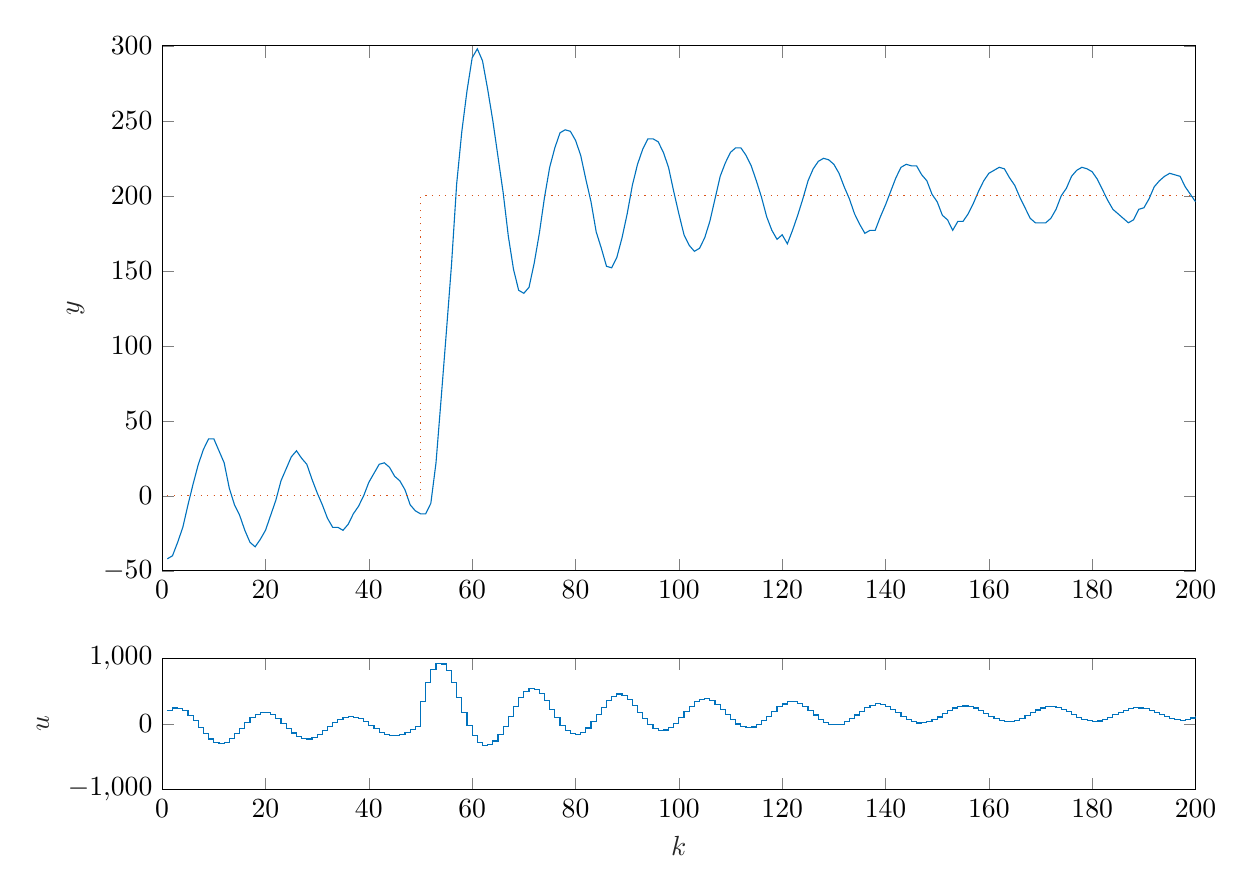
\begin{tikzpicture}

\begin{axis}[%
width=5.167in,
height=0.656in,
at={(0.646in,0.525in)},
scale only axis,
xmin=0,
xmax=200,
xtick={0,20,40,60,80,100,120,140,160,180,200},
xlabel style={font=\color{white!15!black}},
xlabel={$k$},
ymin=-1000,
ymax=1000,
ytick={-1000,0,1000},
ylabel style={font=\color{white!15!black}},
ylabel={$u$},
axis background/.style={fill=white}
]
\addplot[const plot, color=mycolor1, forget plot] table[row sep=crcr] {%
1	204.99\\
2	243.38\\
3	240.99\\
4	204.99\\
5	136.18\\
6	46.96\\
7	-51.95\\
8	-147.21\\
9	-229.25\\
10	-283.35\\
11	-297.55\\
12	-279.37\\
13	-221.11\\
14	-144.31\\
15	-64.15\\
16	18.69\\
17	94.7\\
18	150.85\\
19	174.94\\
20	171.11\\
21	138.33\\
22	84.14\\
23	10.89\\
24	-64.5\\
25	-136.71\\
26	-195.41\\
27	-224.04\\
28	-228.84\\
29	-203.97\\
30	-158.26\\
31	-100.57\\
32	-35.34\\
33	26.83\\
34	72.77\\
35	106.08\\
36	117.41\\
37	104.81\\
38	77.32\\
39	36.31\\
40	-16.67\\
41	-71.06\\
42	-123.12\\
43	-161.52\\
44	-180.24\\
45	-176.66\\
46	-160.35\\
47	-129.75\\
48	-82.5\\
49	-35.47\\
50	347.82\\
51	634.35\\
52	829.45\\
53	926.36\\
54	915.14\\
55	810.42\\
56	635.53\\
57	405\\
58	179.01\\
59	-15.92\\
60	-178.05\\
61	-285.42\\
62	-332.24\\
63	-318.5\\
64	-259.11\\
65	-165.6\\
66	-42.4\\
67	109.33\\
68	263.99\\
69	399.3\\
70	491.12\\
71	537.28\\
72	524.43\\
73	461.97\\
74	354.09\\
75	222.91\\
76	95.88\\
77	-17.37\\
78	-99.77\\
79	-147.54\\
80	-156.21\\
81	-130.1\\
82	-60.72\\
83	32.22\\
84	144.23\\
85	253.53\\
86	356.21\\
87	425.78\\
88	456.92\\
89	437.99\\
90	379.06\\
91	288.45\\
92	182.02\\
93	78.02\\
94	-8.92\\
95	-67.58\\
96	-97.05\\
97	-91.47\\
98	-57.29\\
99	9.33\\
100	95.03\\
101	188.96\\
102	273.09\\
103	340.47\\
104	380.39\\
105	387.81\\
106	361.68\\
107	303.54\\
108	223.45\\
109	140.33\\
110	62.26\\
111	-0.56\\
112	-42.47\\
113	-56.95\\
114	-45.21\\
115	-8.62\\
116	47.76\\
117	120.28\\
118	195.19\\
119	262.65\\
120	305.72\\
121	341.85\\
122	344.76\\
123	319.07\\
124	270.8\\
125	205.39\\
126	136.77\\
127	74.38\\
128	25.59\\
129	-4.27\\
130	-13.74\\
131	-1.46\\
132	32.42\\
133	79.55\\
134	137.8\\
135	197\\
136	251.59\\
137	286.36\\
138	306.86\\
139	299.32\\
140	271.36\\
141	226.89\\
142	171.61\\
143	114.13\\
144	66.89\\
145	35.34\\
146	16.04\\
147	18.32\\
148	33.88\\
149	67.74\\
150	107.42\\
151	156.54\\
152	200.26\\
153	244.75\\
154	265.14\\
155	275.35\\
156	268.39\\
157	244.29\\
158	206.08\\
159	160.93\\
160	115.76\\
161	78.28\\
162	49.13\\
163	32.93\\
164	36.81\\
165	54.34\\
166	86.79\\
167	127.84\\
168	173.77\\
169	214.16\\
170	243.31\\
171	261.81\\
172	265.84\\
173	253\\
174	222.61\\
175	186.61\\
176	142.96\\
177	101.85\\
178	68.17\\
179	47.25\\
180	38.84\\
181	46.03\\
182	68.61\\
183	102.14\\
184	140.82\\
185	177.13\\
186	209.24\\
187	236.77\\
188	250.67\\
189	244.8\\
190	233.85\\
191	211.12\\
192	176.07\\
193	140.5\\
194	107.93\\
195	80.64\\
196	64.4\\
197	57.68\\
198	69.12\\
199	90.99\\
200	120.03\\
};
\end{axis}

\begin{axis}[%
width=5.167in,
height=2.625in,
at={(0.646in,1.619in)},
scale only axis,
xmin=0,
xmax=200,
xtick={0,20,40,60,80,100,120,140,160,180,200},
ymin=-50,
ymax=300,
ytick={-50,0,50,100,150,200,250,300},
ylabel style={font=\color{white!15!black}},
ylabel={$y$},
axis background/.style={fill=white}
]
\addplot [color=mycolor1, forget plot]
  table[row sep=crcr]{%
1	-42\\
2	-40\\
3	-31\\
4	-21\\
5	-6\\
6	8\\
7	21\\
8	31\\
9	38\\
10	38\\
11	30\\
12	22\\
13	5\\
14	-6\\
15	-13\\
16	-23\\
17	-31\\
18	-34\\
19	-29\\
20	-23\\
21	-13\\
22	-3\\
23	10\\
24	18\\
25	26\\
26	30\\
27	25\\
28	21\\
29	11\\
30	2\\
31	-6\\
32	-15\\
33	-21\\
34	-21\\
35	-23\\
36	-19\\
37	-12\\
38	-7\\
39	0\\
40	9\\
41	15\\
42	21\\
43	22\\
44	19\\
45	13\\
46	10\\
47	4\\
48	-6\\
49	-10\\
50	-12\\
51	-12\\
52	-5\\
53	22\\
54	65\\
55	109\\
56	154\\
57	208\\
58	243\\
59	270\\
60	292\\
61	298\\
62	290\\
63	271\\
64	250\\
65	226\\
66	202\\
67	173\\
68	151\\
69	137\\
70	135\\
71	139\\
72	155\\
73	175\\
74	199\\
75	219\\
76	232\\
77	242\\
78	244\\
79	243\\
80	237\\
81	227\\
82	211\\
83	196\\
84	176\\
85	165\\
86	153\\
87	152\\
88	159\\
89	172\\
90	188\\
91	207\\
92	221\\
93	231\\
94	238\\
95	238\\
96	236\\
97	229\\
98	219\\
99	203\\
100	188\\
101	174\\
102	167\\
103	163\\
104	165\\
105	172\\
106	183\\
107	198\\
108	213\\
109	222\\
110	229\\
111	232\\
112	232\\
113	227\\
114	220\\
115	210\\
116	199\\
117	186\\
118	177\\
119	171\\
120	174\\
121	168\\
122	177\\
123	187\\
124	198\\
125	210\\
126	218\\
127	223\\
128	225\\
129	224\\
130	221\\
131	215\\
132	206\\
133	198\\
134	188\\
135	181\\
136	175\\
137	177\\
138	177\\
139	186\\
140	194\\
141	203\\
142	212\\
143	219\\
144	221\\
145	220\\
146	220\\
147	214\\
148	210\\
149	201\\
150	196\\
151	187\\
152	184\\
153	177\\
154	183\\
155	183\\
156	188\\
157	195\\
158	203\\
159	210\\
160	215\\
161	217\\
162	219\\
163	218\\
164	212\\
165	207\\
166	199\\
167	192\\
168	185\\
169	182\\
170	182\\
171	182\\
172	185\\
173	191\\
174	200\\
175	205\\
176	213\\
177	217\\
178	219\\
179	218\\
180	216\\
181	211\\
182	204\\
183	197\\
184	191\\
185	188\\
186	185\\
187	182\\
188	184\\
189	191\\
190	192\\
191	198\\
192	206\\
193	210\\
194	213\\
195	215\\
196	214\\
197	213\\
198	206\\
199	201\\
200	196\\
};
\addplot[const plot, color=mycolor2, dotted, forget plot] table[row sep=crcr] {%
1	0\\
2	0\\
3	0\\
4	0\\
5	0\\
6	0\\
7	0\\
8	0\\
9	0\\
10	0\\
11	0\\
12	0\\
13	0\\
14	0\\
15	0\\
16	0\\
17	0\\
18	0\\
19	0\\
20	0\\
21	0\\
22	0\\
23	0\\
24	0\\
25	0\\
26	0\\
27	0\\
28	0\\
29	0\\
30	0\\
31	0\\
32	0\\
33	0\\
34	0\\
35	0\\
36	0\\
37	0\\
38	0\\
39	0\\
40	0\\
41	0\\
42	0\\
43	0\\
44	0\\
45	0\\
46	0\\
47	0\\
48	0\\
49	0\\
50	200\\
51	200\\
52	200\\
53	200\\
54	200\\
55	200\\
56	200\\
57	200\\
58	200\\
59	200\\
60	200\\
61	200\\
62	200\\
63	200\\
64	200\\
65	200\\
66	200\\
67	200\\
68	200\\
69	200\\
70	200\\
71	200\\
72	200\\
73	200\\
74	200\\
75	200\\
76	200\\
77	200\\
78	200\\
79	200\\
80	200\\
81	200\\
82	200\\
83	200\\
84	200\\
85	200\\
86	200\\
87	200\\
88	200\\
89	200\\
90	200\\
91	200\\
92	200\\
93	200\\
94	200\\
95	200\\
96	200\\
97	200\\
98	200\\
99	200\\
100	200\\
101	200\\
102	200\\
103	200\\
104	200\\
105	200\\
106	200\\
107	200\\
108	200\\
109	200\\
110	200\\
111	200\\
112	200\\
113	200\\
114	200\\
115	200\\
116	200\\
117	200\\
118	200\\
119	200\\
120	200\\
121	200\\
122	200\\
123	200\\
124	200\\
125	200\\
126	200\\
127	200\\
128	200\\
129	200\\
130	200\\
131	200\\
132	200\\
133	200\\
134	200\\
135	200\\
136	200\\
137	200\\
138	200\\
139	200\\
140	200\\
141	200\\
142	200\\
143	200\\
144	200\\
145	200\\
146	200\\
147	200\\
148	200\\
149	200\\
150	200\\
151	200\\
152	200\\
153	200\\
154	200\\
155	200\\
156	200\\
157	200\\
158	200\\
159	200\\
160	200\\
161	200\\
162	200\\
163	200\\
164	200\\
165	200\\
166	200\\
167	200\\
168	200\\
169	200\\
170	200\\
171	200\\
172	200\\
173	200\\
174	200\\
175	200\\
176	200\\
177	200\\
178	200\\
179	200\\
180	200\\
181	200\\
182	200\\
183	200\\
184	200\\
185	200\\
186	200\\
187	200\\
188	200\\
189	200\\
190	200\\
191	200\\
192	200\\
193	200\\
194	200\\
195	200\\
196	200\\
197	200\\
198	200\\
199	200\\
200	200\\
};
\end{axis}
\end{tikzpicture}%
\end{figure}

\begin{figure}[H]
\centering
%err =208462
\definecolor{mycolor1}{rgb}{0.00000,0.44700,0.74100}%
\definecolor{mycolor2}{rgb}{0.85000,0.32500,0.09800}%
%
\begin{tikzpicture}

\begin{axis}[%
width=5.167in,
height=0.656in,
at={(0.646in,0.525in)},
scale only axis,
xmin=0,
xmax=200,
xtick={0,20,40,60,80,100,120,140,160,180,200},
xlabel style={font=\color{white!15!black}},
xlabel={$k$},
ymin=-1000,
ymax=1000,
ytick={-1000,0,1000},
ylabel style={font=\color{white!15!black}},
ylabel={$u$},
axis background/.style={fill=white}
]
\addplot[const plot, color=mycolor1, forget plot] table[row sep=crcr] {%
1	-23.08\\
2	-22.45\\
3	-23.98\\
4	-25.97\\
5	-31.75\\
6	-35.41\\
7	-40.69\\
8	-42.14\\
9	-45.07\\
10	-45.55\\
11	-46.27\\
12	-47.37\\
13	-45.33\\
14	-42.12\\
15	-39.48\\
16	-37.42\\
17	-34.7\\
18	-35.46\\
19	-34.21\\
20	-33.78\\
21	-32.91\\
22	-33.85\\
23	-33.6\\
24	-38.21\\
25	-40.52\\
26	-45.62\\
27	-44.59\\
28	-42.21\\
29	-41.18\\
30	-41.06\\
31	-39.51\\
32	-40.63\\
33	-39.31\\
34	-38.52\\
35	-37.01\\
36	-34.72\\
37	-33.18\\
38	-32.14\\
39	-31.63\\
40	-32.65\\
41	-35.97\\
42	-37.36\\
43	-39.51\\
44	-40.84\\
45	-40.35\\
46	-44.33\\
47	-46\\
48	-44.76\\
49	-42.6\\
50	193.55\\
51	372.37\\
52	494.63\\
53	567.39\\
54	589.31\\
55	559.27\\
56	502.04\\
57	428.22\\
58	340.53\\
59	245.27\\
60	161.3\\
61	91.49\\
62	42.09\\
63	8.48\\
64	-11.51\\
65	-13.2\\
66	0.03\\
67	26.74\\
68	59.81\\
69	94.47\\
70	128.9\\
71	162.16\\
72	186.91\\
73	204.55\\
74	211.8\\
75	207.49\\
76	193.29\\
77	177.49\\
78	159.11\\
79	143.53\\
80	132.46\\
81	121.32\\
82	118.94\\
83	127.16\\
84	138.63\\
85	150.68\\
86	163.32\\
87	173.5\\
88	184.21\\
89	185.22\\
90	182.19\\
91	175.73\\
92	162.88\\
93	149.99\\
94	139.68\\
95	125.11\\
96	120.96\\
97	124.02\\
98	126.43\\
99	132.23\\
100	139.15\\
101	146.09\\
102	152.29\\
103	158.81\\
104	162.82\\
105	167.14\\
106	165.65\\
107	166.65\\
108	162.45\\
109	156.93\\
110	148.42\\
111	145.12\\
112	140.44\\
113	137.4\\
114	136.17\\
115	134.12\\
116	132.43\\
117	132.01\\
118	138.31\\
119	142.23\\
120	148.95\\
121	153.85\\
122	158.07\\
123	159.29\\
124	159.17\\
125	159.22\\
126	157.43\\
127	156.76\\
128	151.54\\
129	146.74\\
130	139.87\\
131	139.81\\
132	140.35\\
133	143.5\\
134	146.64\\
135	148.33\\
136	150.83\\
137	151.53\\
138	151.68\\
139	153.76\\
140	155.12\\
141	154.79\\
142	154.27\\
143	153.86\\
144	152.09\\
145	150.55\\
146	149.27\\
147	148.41\\
148	149.2\\
149	146.61\\
150	141.5\\
151	139.06\\
152	139.81\\
153	142.77\\
154	145.17\\
155	147.1\\
156	150.93\\
157	155.87\\
158	156.8\\
159	157.04\\
160	156.87\\
161	152.97\\
162	147.53\\
163	143.53\\
164	137.15\\
165	136.14\\
166	137.99\\
167	139.62\\
168	144.59\\
169	147.41\\
170	151.79\\
171	154.96\\
172	157.07\\
173	157.22\\
174	158.45\\
175	154.57\\
176	155.06\\
177	153.07\\
178	152.62\\
179	148.76\\
180	148.23\\
181	145.53\\
182	144.69\\
183	143.17\\
184	142.28\\
185	139.55\\
186	138.91\\
187	142.15\\
188	145.86\\
189	147.58\\
190	149.92\\
191	153.82\\
192	155.23\\
193	156.97\\
194	156.75\\
195	156.35\\
196	153.46\\
197	150.1\\
198	145.32\\
199	139.48\\
200	137.76\\
};
\end{axis}

\begin{axis}[%
width=5.167in,
height=2.625in,
at={(0.646in,1.619in)},
scale only axis,
xmin=0,
xmax=200,
xtick={0,20,40,60,80,100,120,140,160,180,200},
ymin=-50,
ymax=250,
ytick={-50,0,50,100,150,200,250},
ylabel style={font=\color{white!15!black}},
ylabel={$y$},
axis background/.style={fill=white}
]
\addplot [color=mycolor1, forget plot]
  table[row sep=crcr]{%
1	-4\\
2	-3\\
3	-2\\
4	-2\\
5	1\\
6	0\\
7	2\\
8	0\\
9	2\\
10	1\\
11	2\\
12	3\\
13	1\\
14	0\\
15	0\\
16	0\\
17	-1\\
18	1\\
19	-1\\
20	-1\\
21	-2\\
22	-1\\
23	-2\\
24	2\\
25	1\\
26	4\\
27	0\\
28	-1\\
29	0\\
30	1\\
31	0\\
32	2\\
33	0\\
34	0\\
35	-1\\
36	-2\\
37	-2\\
38	-2\\
39	-2\\
40	-1\\
41	1\\
42	0\\
43	1\\
44	1\\
45	0\\
46	4\\
47	3\\
48	1\\
49	0\\
50	1\\
51	1\\
52	10\\
53	27\\
54	53\\
55	87\\
56	112\\
57	139\\
58	172\\
59	207\\
60	227\\
61	242\\
62	246\\
63	249\\
64	250\\
65	243\\
66	237\\
67	228\\
68	220\\
69	212\\
70	202\\
71	192\\
72	187\\
73	183\\
74	182\\
75	184\\
76	189\\
77	190\\
78	194\\
79	196\\
80	198\\
81	203\\
82	204\\
83	200\\
84	198\\
85	198\\
86	197\\
87	196\\
88	194\\
89	197\\
90	198\\
91	200\\
92	204\\
93	205\\
94	206\\
95	212\\
96	207\\
97	204\\
98	205\\
99	203\\
100	202\\
101	201\\
102	200\\
103	198\\
104	198\\
105	196\\
106	199\\
107	196\\
108	199\\
109	200\\
110	203\\
111	200\\
112	202\\
113	202\\
114	202\\
115	204\\
116	205\\
117	205\\
118	200\\
119	201\\
120	198\\
121	198\\
122	197\\
123	198\\
124	198\\
125	197\\
126	198\\
127	197\\
128	201\\
129	202\\
130	205\\
131	201\\
132	201\\
133	199\\
134	199\\
135	200\\
136	199\\
137	200\\
138	200\\
139	198\\
140	198\\
141	199\\
142	199\\
143	199\\
144	200\\
145	200\\
146	200\\
147	200\\
148	199\\
149	202\\
150	205\\
151	204\\
152	202\\
153	200\\
154	200\\
155	200\\
156	198\\
157	196\\
158	198\\
159	198\\
160	198\\
161	201\\
162	203\\
163	203\\
164	206\\
165	203\\
166	201\\
167	201\\
168	198\\
169	199\\
170	197\\
171	197\\
172	197\\
173	198\\
174	197\\
175	201\\
176	198\\
177	200\\
178	199\\
179	202\\
180	200\\
181	202\\
182	201\\
183	202\\
184	202\\
185	204\\
186	203\\
187	200\\
188	199\\
189	200\\
190	199\\
191	197\\
192	198\\
193	197\\
194	198\\
195	198\\
196	200\\
197	201\\
198	203\\
199	205\\
200	203\\
};
\addplot[const plot, color=mycolor2, dotted, forget plot] table[row sep=crcr] {%
1	0\\
2	0\\
3	0\\
4	0\\
5	0\\
6	0\\
7	0\\
8	0\\
9	0\\
10	0\\
11	0\\
12	0\\
13	0\\
14	0\\
15	0\\
16	0\\
17	0\\
18	0\\
19	0\\
20	0\\
21	0\\
22	0\\
23	0\\
24	0\\
25	0\\
26	0\\
27	0\\
28	0\\
29	0\\
30	0\\
31	0\\
32	0\\
33	0\\
34	0\\
35	0\\
36	0\\
37	0\\
38	0\\
39	0\\
40	0\\
41	0\\
42	0\\
43	0\\
44	0\\
45	0\\
46	0\\
47	0\\
48	0\\
49	0\\
50	200\\
51	200\\
52	200\\
53	200\\
54	200\\
55	200\\
56	200\\
57	200\\
58	200\\
59	200\\
60	200\\
61	200\\
62	200\\
63	200\\
64	200\\
65	200\\
66	200\\
67	200\\
68	200\\
69	200\\
70	200\\
71	200\\
72	200\\
73	200\\
74	200\\
75	200\\
76	200\\
77	200\\
78	200\\
79	200\\
80	200\\
81	200\\
82	200\\
83	200\\
84	200\\
85	200\\
86	200\\
87	200\\
88	200\\
89	200\\
90	200\\
91	200\\
92	200\\
93	200\\
94	200\\
95	200\\
96	200\\
97	200\\
98	200\\
99	200\\
100	200\\
101	200\\
102	200\\
103	200\\
104	200\\
105	200\\
106	200\\
107	200\\
108	200\\
109	200\\
110	200\\
111	200\\
112	200\\
113	200\\
114	200\\
115	200\\
116	200\\
117	200\\
118	200\\
119	200\\
120	200\\
121	200\\
122	200\\
123	200\\
124	200\\
125	200\\
126	200\\
127	200\\
128	200\\
129	200\\
130	200\\
131	200\\
132	200\\
133	200\\
134	200\\
135	200\\
136	200\\
137	200\\
138	200\\
139	200\\
140	200\\
141	200\\
142	200\\
143	200\\
144	200\\
145	200\\
146	200\\
147	200\\
148	200\\
149	200\\
150	200\\
151	200\\
152	200\\
153	200\\
154	200\\
155	200\\
156	200\\
157	200\\
158	200\\
159	200\\
160	200\\
161	200\\
162	200\\
163	200\\
164	200\\
165	200\\
166	200\\
167	200\\
168	200\\
169	200\\
170	200\\
171	200\\
172	200\\
173	200\\
174	200\\
175	200\\
176	200\\
177	200\\
178	200\\
179	200\\
180	200\\
181	200\\
182	200\\
183	200\\
184	200\\
185	200\\
186	200\\
187	200\\
188	200\\
189	200\\
190	200\\
191	200\\
192	200\\
193	200\\
194	200\\
195	200\\
196	200\\
197	200\\
198	200\\
199	200\\
200	200\\
};
\end{axis}
\end{tikzpicture}%
\end{figure}

\begin{figure}[H]
\centering
%err =207419
\definecolor{mycolor1}{rgb}{0.00000,0.44700,0.74100}%
\definecolor{mycolor2}{rgb}{0.85000,0.32500,0.09800}%
%
\begin{tikzpicture}

\begin{axis}[%
width=5.167in,
height=0.656in,
at={(0.646in,0.525in)},
scale only axis,
xmin=0,
xmax=200,
xtick={0,20,40,60,80,100,120,140,160,180,200},
xlabel style={font=\color{white!15!black}},
xlabel={$k$},
ymin=-1000,
ymax=1000,
ytick={-1000,0,1000},
ylabel style={font=\color{white!15!black}},
ylabel={$u$},
axis background/.style={fill=white}
]
\addplot[const plot, color=mycolor1, forget plot] table[row sep=crcr] {%
1	-20.93\\
2	-20.11\\
3	-21.94\\
4	-25.66\\
5	-30.74\\
6	-35.25\\
7	-41.4\\
8	-46.1\\
9	-47.97\\
10	-52.29\\
11	-51.03\\
12	-52.44\\
13	-47.98\\
14	-42.59\\
15	-38.02\\
16	-35.71\\
17	-32.86\\
18	-30.12\\
19	-30.06\\
20	-30.83\\
21	-32.11\\
22	-36.1\\
23	-35.92\\
24	-40.75\\
25	-42.05\\
26	-43.8\\
27	-48.29\\
28	-44.13\\
29	-42.66\\
30	-41.1\\
31	-37.06\\
32	-33.69\\
33	-31.33\\
34	-29.65\\
35	-31.13\\
36	-35.05\\
37	-37.23\\
38	-42.8\\
39	-46.09\\
40	-46.21\\
41	-44.95\\
42	-43.83\\
43	-40.4\\
44	-38.71\\
45	-36.17\\
46	-36.47\\
47	-37.87\\
48	-36.61\\
49	-36.66\\
50	198.52\\
51	378.82\\
52	505.86\\
53	580.32\\
54	608.74\\
55	583.12\\
56	524.19\\
57	443.38\\
58	345.83\\
59	246.6\\
60	158.98\\
61	81.69\\
62	21.63\\
63	-16.16\\
64	-36.36\\
65	-37.71\\
66	-20.74\\
67	11.26\\
68	43.57\\
69	86.71\\
70	129.16\\
71	167.08\\
72	196.27\\
73	213.04\\
74	223.14\\
75	217.62\\
76	204.78\\
77	188.01\\
78	165.93\\
79	146.99\\
80	133.28\\
81	116.83\\
82	110.83\\
83	117.24\\
84	127.1\\
85	138.81\\
86	154.51\\
87	165.3\\
88	178.96\\
89	183.16\\
90	183.19\\
91	178.27\\
92	168.27\\
93	156.69\\
94	148.81\\
95	138.08\\
96	123.5\\
97	125.69\\
98	125.44\\
99	130.79\\
100	137.95\\
101	144.87\\
102	151.86\\
103	160.61\\
104	164.24\\
105	166.98\\
106	166.63\\
107	165.99\\
108	160.29\\
109	156.92\\
110	151.04\\
111	144.74\\
112	139.83\\
113	136.37\\
114	134.57\\
115	135.61\\
116	132.93\\
117	133.08\\
118	139.03\\
119	145.13\\
120	153.77\\
121	159.14\\
122	163.75\\
123	165.38\\
124	165.53\\
125	162.01\\
126	157.44\\
127	153.42\\
128	148.87\\
129	143.43\\
130	139.68\\
131	133.84\\
132	137.17\\
133	136.77\\
134	142.81\\
135	147.11\\
136	150.5\\
137	151.95\\
138	154.04\\
139	152.68\\
140	152.18\\
141	150.37\\
142	149.6\\
143	149.98\\
144	150.08\\
145	151.17\\
146	149.57\\
147	148.37\\
148	148.72\\
149	147.99\\
150	144.34\\
151	141.96\\
152	145.26\\
153	146.88\\
154	146.95\\
155	148.29\\
156	146.88\\
157	150.09\\
158	149.88\\
159	149.35\\
160	147.6\\
161	146.16\\
162	147.36\\
163	148.16\\
164	147.79\\
165	141.69\\
166	144.31\\
167	147.57\\
168	150.09\\
169	152.11\\
170	152.76\\
171	153.15\\
172	154.41\\
173	152.79\\
174	150.17\\
175	150.64\\
176	151.03\\
177	150.09\\
178	149.52\\
179	148.02\\
180	149.31\\
181	149.09\\
182	148.83\\
183	150.01\\
184	148.78\\
185	146.77\\
186	142.82\\
187	144.56\\
188	144.67\\
189	148.42\\
190	147.81\\
191	149.58\\
192	150.91\\
193	150.49\\
194	153.46\\
195	153.26\\
196	153.05\\
197	151.65\\
198	150.77\\
199	146.57\\
200	140.93\\
};
\end{axis}

\begin{axis}[%
width=5.167in,
height=2.625in,
at={(0.646in,1.619in)},
scale only axis,
xmin=0,
xmax=200,
xtick={0,20,40,60,80,100,120,140,160,180,200},
ymin=-50,
ymax=300,
ytick={-50,0,50,100,150,200,250,300},
ylabel style={font=\color{white!15!black}},
ylabel={$y$},
axis background/.style={fill=white}
]
\addplot [color=mycolor1, forget plot]
  table[row sep=crcr]{%
1	-3\\
2	-3\\
3	-2\\
4	-1\\
5	0\\
6	0\\
7	2\\
8	2\\
9	1\\
10	4\\
11	1\\
12	4\\
13	0\\
14	-1\\
15	-1\\
16	0\\
17	-1\\
18	-2\\
19	-1\\
20	-1\\
21	-1\\
22	1\\
23	-2\\
24	2\\
25	0\\
26	1\\
27	4\\
28	-2\\
29	0\\
30	0\\
31	-2\\
32	-2\\
33	-2\\
34	-2\\
35	0\\
36	2\\
37	1\\
38	4\\
39	3\\
40	1\\
41	0\\
42	0\\
43	-2\\
44	-1\\
45	-2\\
46	0\\
47	1\\
48	-1\\
49	0\\
50	2\\
51	3\\
52	11\\
53	31\\
54	53\\
55	87\\
56	115\\
57	145\\
58	180\\
59	210\\
60	229\\
61	247\\
62	255\\
63	255\\
64	254\\
65	247\\
66	239\\
67	229\\
68	226\\
69	211\\
70	200\\
71	191\\
72	185\\
73	184\\
74	179\\
75	183\\
76	185\\
77	187\\
78	193\\
79	195\\
80	197\\
81	205\\
82	206\\
83	202\\
84	201\\
85	201\\
86	198\\
87	199\\
88	195\\
89	197\\
90	197\\
91	199\\
92	201\\
93	202\\
94	201\\
95	205\\
96	211\\
97	202\\
98	205\\
99	202\\
100	201\\
101	201\\
102	200\\
103	197\\
104	199\\
105	198\\
106	199\\
107	198\\
108	201\\
109	199\\
110	201\\
111	202\\
112	202\\
113	202\\
114	202\\
115	201\\
116	205\\
117	204\\
118	200\\
119	199\\
120	196\\
121	197\\
122	196\\
123	197\\
124	197\\
125	199\\
126	200\\
127	200\\
128	201\\
129	203\\
130	203\\
131	206\\
132	200\\
133	203\\
134	198\\
135	199\\
136	199\\
137	200\\
138	199\\
139	201\\
140	200\\
141	201\\
142	200\\
143	199\\
144	199\\
145	198\\
146	200\\
147	200\\
148	199\\
149	200\\
150	203\\
151	203\\
152	199\\
153	200\\
154	201\\
155	200\\
156	202\\
157	198\\
158	200\\
159	200\\
160	201\\
161	201\\
162	199\\
163	199\\
164	200\\
165	205\\
166	199\\
167	198\\
168	198\\
169	198\\
170	199\\
171	199\\
172	198\\
173	200\\
174	201\\
175	199\\
176	199\\
177	200\\
178	200\\
179	201\\
180	199\\
181	200\\
182	200\\
183	199\\
184	201\\
185	202\\
186	204\\
187	200\\
188	201\\
189	198\\
190	201\\
191	199\\
192	199\\
193	200\\
194	197\\
195	199\\
196	199\\
197	200\\
198	200\\
199	203\\
200	205\\
};
\addplot[const plot, color=mycolor2, dotted, forget plot] table[row sep=crcr] {%
1	0\\
2	0\\
3	0\\
4	0\\
5	0\\
6	0\\
7	0\\
8	0\\
9	0\\
10	0\\
11	0\\
12	0\\
13	0\\
14	0\\
15	0\\
16	0\\
17	0\\
18	0\\
19	0\\
20	0\\
21	0\\
22	0\\
23	0\\
24	0\\
25	0\\
26	0\\
27	0\\
28	0\\
29	0\\
30	0\\
31	0\\
32	0\\
33	0\\
34	0\\
35	0\\
36	0\\
37	0\\
38	0\\
39	0\\
40	0\\
41	0\\
42	0\\
43	0\\
44	0\\
45	0\\
46	0\\
47	0\\
48	0\\
49	0\\
50	200\\
51	200\\
52	200\\
53	200\\
54	200\\
55	200\\
56	200\\
57	200\\
58	200\\
59	200\\
60	200\\
61	200\\
62	200\\
63	200\\
64	200\\
65	200\\
66	200\\
67	200\\
68	200\\
69	200\\
70	200\\
71	200\\
72	200\\
73	200\\
74	200\\
75	200\\
76	200\\
77	200\\
78	200\\
79	200\\
80	200\\
81	200\\
82	200\\
83	200\\
84	200\\
85	200\\
86	200\\
87	200\\
88	200\\
89	200\\
90	200\\
91	200\\
92	200\\
93	200\\
94	200\\
95	200\\
96	200\\
97	200\\
98	200\\
99	200\\
100	200\\
101	200\\
102	200\\
103	200\\
104	200\\
105	200\\
106	200\\
107	200\\
108	200\\
109	200\\
110	200\\
111	200\\
112	200\\
113	200\\
114	200\\
115	200\\
116	200\\
117	200\\
118	200\\
119	200\\
120	200\\
121	200\\
122	200\\
123	200\\
124	200\\
125	200\\
126	200\\
127	200\\
128	200\\
129	200\\
130	200\\
131	200\\
132	200\\
133	200\\
134	200\\
135	200\\
136	200\\
137	200\\
138	200\\
139	200\\
140	200\\
141	200\\
142	200\\
143	200\\
144	200\\
145	200\\
146	200\\
147	200\\
148	200\\
149	200\\
150	200\\
151	200\\
152	200\\
153	200\\
154	200\\
155	200\\
156	200\\
157	200\\
158	200\\
159	200\\
160	200\\
161	200\\
162	200\\
163	200\\
164	200\\
165	200\\
166	200\\
167	200\\
168	200\\
169	200\\
170	200\\
171	200\\
172	200\\
173	200\\
174	200\\
175	200\\
176	200\\
177	200\\
178	200\\
179	200\\
180	200\\
181	200\\
182	200\\
183	200\\
184	200\\
185	200\\
186	200\\
187	200\\
188	200\\
189	200\\
190	200\\
191	200\\
192	200\\
193	200\\
194	200\\
195	200\\
196	200\\
197	200\\
198	200\\
199	200\\
200	200\\
};
\end{axis}
\end{tikzpicture}%
\end{figure}

\begin{figure}[H]
\centering
%err =205676
\definecolor{mycolor1}{rgb}{0.00000,0.44700,0.74100}%
\definecolor{mycolor2}{rgb}{0.85000,0.32500,0.09800}%
%
\begin{tikzpicture}

\begin{axis}[%
width=5.167in,
height=0.656in,
at={(0.646in,0.525in)},
scale only axis,
xmin=0,
xmax=200,
xtick={0,20,40,60,80,100,120,140,160,180,200},
xlabel style={font=\color{white!15!black}},
xlabel={$k$},
ymin=-1000,
ymax=1000,
ytick={-1000,0,1000},
ylabel style={font=\color{white!15!black}},
ylabel={$u$},
axis background/.style={fill=white}
]
\addplot[const plot, color=mycolor1, forget plot] table[row sep=crcr] {%
1	-27.27\\
2	-26.26\\
3	-26.6\\
4	-30.28\\
5	-32.62\\
6	-36.02\\
7	-38.74\\
8	-41.78\\
9	-42.55\\
10	-43.92\\
11	-44.48\\
12	-45.64\\
13	-45.93\\
14	-40.86\\
15	-37.85\\
16	-36.64\\
17	-34.45\\
18	-34.32\\
19	-34.63\\
20	-35.38\\
21	-36.45\\
22	-39.96\\
23	-40.35\\
24	-40.78\\
25	-39.88\\
26	-40.28\\
27	-39.26\\
28	-40.58\\
29	-41.36\\
30	-45.31\\
31	-42.19\\
32	-40.76\\
33	-38.48\\
34	-36.66\\
35	-35.36\\
36	-34.68\\
37	-33.3\\
38	-34.97\\
39	-35.42\\
40	-35.71\\
41	-35.91\\
42	-35.98\\
43	-35.82\\
44	-35.55\\
45	-37.61\\
46	-39.04\\
47	-43.51\\
48	-40.94\\
49	-39.96\\
50	196.36\\
51	373.89\\
52	498.38\\
53	569.84\\
54	590.91\\
55	563.81\\
56	505.09\\
57	429.69\\
58	339.23\\
59	247.19\\
60	166.16\\
61	99.25\\
62	47.02\\
63	8.64\\
64	-16.23\\
65	-24.19\\
66	-10.93\\
67	16.31\\
68	50.29\\
69	88.68\\
70	126.26\\
71	159.48\\
72	186.34\\
73	202.9\\
74	212.34\\
75	209.52\\
76	199.74\\
77	183.53\\
78	165.83\\
79	150.3\\
80	137.62\\
81	123.79\\
82	119.35\\
83	126.18\\
84	134.67\\
85	147.14\\
86	159.32\\
87	167.17\\
88	176.32\\
89	177.43\\
90	174.52\\
91	169.3\\
92	160.98\\
93	152.66\\
94	144.23\\
95	136.76\\
96	130.56\\
97	129.27\\
98	129.36\\
99	127.48\\
100	134.38\\
101	141.72\\
102	148.66\\
103	156.03\\
104	159.9\\
105	160.49\\
106	163.17\\
107	162.54\\
108	159.38\\
109	154.8\\
110	149.41\\
111	147.32\\
112	144.55\\
113	141.5\\
114	141.19\\
115	140.73\\
116	137.69\\
117	136.28\\
118	140.77\\
119	144.6\\
120	147.81\\
121	152.62\\
122	154.64\\
123	155.66\\
124	154.46\\
125	154.99\\
126	153.67\\
127	152.26\\
128	153.45\\
129	152.21\\
130	151.44\\
131	151.05\\
132	148.78\\
133	143.77\\
134	142.67\\
135	143.47\\
136	145.51\\
137	146.08\\
138	146.75\\
139	147.12\\
140	149.38\\
141	150.81\\
142	150.31\\
143	152.08\\
144	153.45\\
145	154.26\\
146	153.63\\
147	152.05\\
148	150.77\\
149	149.81\\
150	144.49\\
151	141.82\\
152	141.26\\
153	143.41\\
154	145.16\\
155	147.79\\
156	147.47\\
157	149.51\\
158	150.88\\
159	150.45\\
160	149.97\\
161	149.58\\
162	150.43\\
163	149.85\\
164	151.7\\
165	149.51\\
166	149.01\\
167	145.02\\
168	143.14\\
169	139.45\\
170	141.51\\
171	145.69\\
172	147.9\\
173	149.67\\
174	152.21\\
175	154.04\\
176	153.91\\
177	153.55\\
178	153.19\\
179	152.87\\
180	153.83\\
181	153.47\\
182	151.92\\
183	150.75\\
184	147.53\\
185	142.73\\
186	140.36\\
187	142.46\\
188	143.06\\
189	145.02\\
190	146.75\\
191	149.23\\
192	150.95\\
193	149.66\\
194	150.78\\
195	151.46\\
196	153.06\\
197	154.16\\
198	154.99\\
199	154.33\\
200	153.73\\
};
\end{axis}

\begin{axis}[%
width=5.167in,
height=2.625in,
at={(0.646in,1.619in)},
scale only axis,
xmin=0,
xmax=200,
xtick={0,20,40,60,80,100,120,140,160,180,200},
ymin=-50,
ymax=300,
ytick={-50,0,50,100,150,200,250,300},
ylabel style={font=\color{white!15!black}},
ylabel={$y$},
axis background/.style={fill=white}
]
\addplot [color=mycolor1, forget plot]
  table[row sep=crcr]{%
1	-2\\
2	-2\\
3	-2\\
4	0\\
5	-1\\
6	0\\
7	0\\
8	1\\
9	0\\
10	1\\
11	1\\
12	2\\
13	2\\
14	-2\\
15	-1\\
16	0\\
17	-1\\
18	0\\
19	0\\
20	0\\
21	0\\
22	2\\
23	0\\
24	0\\
25	-1\\
26	0\\
27	-1\\
28	1\\
29	1\\
30	4\\
31	-1\\
32	0\\
33	-1\\
34	-1\\
35	-1\\
36	-1\\
37	-2\\
38	0\\
39	-1\\
40	-1\\
41	-1\\
42	-1\\
43	-1\\
44	-1\\
45	1\\
46	1\\
47	4\\
48	-1\\
49	0\\
50	1\\
51	3\\
52	10\\
53	30\\
54	56\\
55	87\\
56	115\\
57	142\\
58	176\\
59	206\\
60	225\\
61	239\\
62	247\\
63	252\\
64	254\\
65	249\\
66	239\\
67	230\\
68	222\\
69	212\\
70	202\\
71	194\\
72	187\\
73	185\\
74	181\\
75	183\\
76	185\\
77	189\\
78	192\\
79	194\\
80	197\\
81	203\\
82	204\\
83	200\\
84	200\\
85	198\\
86	198\\
87	199\\
88	197\\
89	199\\
90	200\\
91	201\\
92	202\\
93	202\\
94	204\\
95	205\\
96	206\\
97	205\\
98	205\\
99	208\\
100	202\\
101	201\\
102	200\\
103	198\\
104	199\\
105	200\\
106	197\\
107	198\\
108	199\\
109	200\\
110	201\\
111	199\\
112	200\\
113	201\\
114	200\\
115	201\\
116	204\\
117	204\\
118	200\\
119	200\\
120	200\\
121	198\\
122	199\\
123	199\\
124	200\\
125	198\\
126	199\\
127	199\\
128	197\\
129	199\\
130	199\\
131	199\\
132	201\\
133	204\\
134	202\\
135	201\\
136	200\\
137	201\\
138	201\\
139	201\\
140	199\\
141	199\\
142	200\\
143	198\\
144	198\\
145	198\\
146	199\\
147	200\\
148	200\\
149	200\\
150	204\\
151	203\\
152	202\\
153	200\\
154	200\\
155	199\\
156	201\\
157	199\\
158	199\\
159	200\\
160	200\\
161	200\\
162	199\\
163	200\\
164	198\\
165	201\\
166	200\\
167	203\\
168	202\\
169	204\\
170	200\\
171	198\\
172	199\\
173	199\\
174	198\\
175	198\\
176	199\\
177	199\\
178	199\\
179	199\\
180	198\\
181	199\\
182	200\\
183	200\\
184	202\\
185	204\\
186	203\\
187	200\\
188	201\\
189	200\\
190	200\\
191	199\\
192	199\\
193	201\\
194	199\\
195	199\\
196	198\\
197	198\\
198	198\\
199	199\\
200	199\\
};
\addplot[const plot, color=mycolor2, dotted, forget plot] table[row sep=crcr] {%
1	0\\
2	0\\
3	0\\
4	0\\
5	0\\
6	0\\
7	0\\
8	0\\
9	0\\
10	0\\
11	0\\
12	0\\
13	0\\
14	0\\
15	0\\
16	0\\
17	0\\
18	0\\
19	0\\
20	0\\
21	0\\
22	0\\
23	0\\
24	0\\
25	0\\
26	0\\
27	0\\
28	0\\
29	0\\
30	0\\
31	0\\
32	0\\
33	0\\
34	0\\
35	0\\
36	0\\
37	0\\
38	0\\
39	0\\
40	0\\
41	0\\
42	0\\
43	0\\
44	0\\
45	0\\
46	0\\
47	0\\
48	0\\
49	0\\
50	200\\
51	200\\
52	200\\
53	200\\
54	200\\
55	200\\
56	200\\
57	200\\
58	200\\
59	200\\
60	200\\
61	200\\
62	200\\
63	200\\
64	200\\
65	200\\
66	200\\
67	200\\
68	200\\
69	200\\
70	200\\
71	200\\
72	200\\
73	200\\
74	200\\
75	200\\
76	200\\
77	200\\
78	200\\
79	200\\
80	200\\
81	200\\
82	200\\
83	200\\
84	200\\
85	200\\
86	200\\
87	200\\
88	200\\
89	200\\
90	200\\
91	200\\
92	200\\
93	200\\
94	200\\
95	200\\
96	200\\
97	200\\
98	200\\
99	200\\
100	200\\
101	200\\
102	200\\
103	200\\
104	200\\
105	200\\
106	200\\
107	200\\
108	200\\
109	200\\
110	200\\
111	200\\
112	200\\
113	200\\
114	200\\
115	200\\
116	200\\
117	200\\
118	200\\
119	200\\
120	200\\
121	200\\
122	200\\
123	200\\
124	200\\
125	200\\
126	200\\
127	200\\
128	200\\
129	200\\
130	200\\
131	200\\
132	200\\
133	200\\
134	200\\
135	200\\
136	200\\
137	200\\
138	200\\
139	200\\
140	200\\
141	200\\
142	200\\
143	200\\
144	200\\
145	200\\
146	200\\
147	200\\
148	200\\
149	200\\
150	200\\
151	200\\
152	200\\
153	200\\
154	200\\
155	200\\
156	200\\
157	200\\
158	200\\
159	200\\
160	200\\
161	200\\
162	200\\
163	200\\
164	200\\
165	200\\
166	200\\
167	200\\
168	200\\
169	200\\
170	200\\
171	200\\
172	200\\
173	200\\
174	200\\
175	200\\
176	200\\
177	200\\
178	200\\
179	200\\
180	200\\
181	200\\
182	200\\
183	200\\
184	200\\
185	200\\
186	200\\
187	200\\
188	200\\
189	200\\
190	200\\
191	200\\
192	200\\
193	200\\
194	200\\
195	200\\
196	200\\
197	200\\
198	200\\
199	200\\
200	200\\
};
\end{axis}
\end{tikzpicture}%
\end{figure}

\chapter{Porównanie najlepszych realizacji}


\begin{figure}[H]
\centering
%err =88754
\definecolor{mycolor1}{rgb}{0.00000,0.44700,0.74100}%
\definecolor{mycolor2}{rgb}{0.85000,0.32500,0.09800}%
%
\begin{tikzpicture}

\begin{axis}[%
width=5.167in,
height=0.656in,
at={(0.646in,0.525in)},
scale only axis,
xmin=0,
xmax=200,
xtick={0,20,40,60,80,100,120,140,160,180,200},
xlabel style={font=\color{white!15!black}},
xlabel={$k$},
ymin=-5000,
ymax=5000,
ytick={-5000,0,5000},
ylabel style={font=\color{white!15!black}},
ylabel={$u$},
axis background/.style={fill=white}
]
\addplot[const plot, color=mycolor1, forget plot] table[row sep=crcr] {%
1	-68.44\\
2	17.87\\
3	4.44\\
4	-59.06\\
5	14.94\\
6	-61.06\\
7	-37.19\\
8	-38.31\\
9	-14.38\\
10	-52.94\\
11	-16.5\\
12	-4.94\\
13	-118.56\\
14	-44.88\\
15	16.56\\
16	-21.81\\
17	-47.75\\
18	-36.25\\
19	-37.25\\
20	-38.25\\
21	-14.19\\
22	-27.56\\
23	-53.5\\
24	-16.94\\
25	-55.38\\
26	-18.81\\
27	-7.13\\
28	4.69\\
29	-33.5\\
30	-71.88\\
31	-98\\
32	-49.19\\
33	-12.69\\
34	-38.56\\
35	-39.44\\
36	9.81\\
37	-40.88\\
38	-79.25\\
39	-30.19\\
40	56.69\\
41	-18.75\\
42	-31.81\\
43	-70.06\\
44	-71\\
45	-59.5\\
46	-35.44\\
47	-48.81\\
48	0.44\\
49	-50.25\\
50	2047\\
51	1984.63\\
52	564.63\\
53	-0.69\\
54	-660.5\\
55	-575.25\\
56	-304.06\\
57	-44.81\\
58	253.62\\
59	391.5\\
60	393.19\\
61	182.5\\
62	171.31\\
63	109.69\\
64	110.19\\
65	135.56\\
66	60.75\\
67	98.25\\
68	123.31\\
69	211.19\\
70	136.75\\
71	224.94\\
72	113.12\\
73	176.19\\
74	139.25\\
75	177.31\\
76	115.31\\
77	140.69\\
78	141.06\\
79	166.5\\
80	104.37\\
81	104.56\\
82	192.37\\
83	105.25\\
84	155.56\\
85	193.56\\
86	169.19\\
87	169.81\\
88	170.44\\
89	95.87\\
90	133.62\\
91	133.87\\
92	184.25\\
93	134.69\\
94	122.5\\
95	135.25\\
96	110.44\\
97	223.31\\
98	148.87\\
99	161.87\\
100	137.31\\
101	175.25\\
102	113.12\\
103	88.25\\
104	138.31\\
105	176.06\\
106	176.5\\
107	139.44\\
108	177.37\\
109	165.37\\
110	140.81\\
111	178.75\\
112	116.62\\
113	116.81\\
114	154.5\\
115	142.25\\
116	142.5\\
117	167.81\\
118	80.5\\
119	143.06\\
120	230.94\\
121	156.5\\
122	144.44\\
123	132.25\\
124	119.94\\
125	207.75\\
126	120.62\\
127	120.81\\
128	158.5\\
129	96.12\\
130	96.06\\
131	208.69\\
132	234.25\\
133	172.44\\
134	135.44\\
135	110.69\\
136	110.75\\
137	123.25\\
138	173.37\\
139	123.56\\
140	186.31\\
141	161.69\\
142	162.06\\
143	162.44\\
144	112.69\\
145	162.87\\
146	150.62\\
147	150.87\\
148	151.12\\
149	126.31\\
150	113.87\\
151	151.44\\
152	114\\
153	151.56\\
154	214.37\\
155	152.31\\
156	165.19\\
157	140.5\\
158	103.12\\
159	153.19\\
160	165.87\\
161	128.56\\
162	191.31\\
163	91.5\\
164	179.12\\
165	104.25\\
166	204.44\\
167	142.25\\
168	180.06\\
169	167.94\\
170	118.19\\
171	118.25\\
172	155.81\\
173	143.44\\
174	118.5\\
175	181.12\\
176	156.37\\
177	181.69\\
178	144.5\\
179	157.25\\
180	132.44\\
181	145.06\\
182	145.19\\
183	170.37\\
184	133.06\\
185	170.75\\
186	83.31\\
187	120.69\\
188	145.62\\
189	158.19\\
190	170.87\\
191	158.62\\
192	209\\
193	159.44\\
194	147.25\\
195	109.87\\
196	134.87\\
197	159.94\\
198	122.5\\
199	135\\
200	135\\
};
\end{axis}

\begin{axis}[%
width=5.167in,
height=2.625in,
at={(0.646in,1.619in)},
scale only axis,
xmin=0,
xmax=200,
xtick={0,20,40,60,80,100,120,140,160,180,200},
ymin=0,
ymax=250,
ytick={0,50,100,150,200,250},
ylabel style={font=\color{white!15!black}},
ylabel={$y$},
axis background/.style={fill=white}
]
\addplot [color=mycolor1, forget plot]
  table[row sep=crcr]{%
1	11\\
2	8\\
3	7\\
4	9\\
5	7\\
6	9\\
7	9\\
8	9\\
9	8\\
10	9\\
11	8\\
12	7\\
13	11\\
14	10\\
15	7\\
16	7\\
17	8\\
18	8\\
19	8\\
20	8\\
21	7\\
22	7\\
23	8\\
24	7\\
25	8\\
26	7\\
27	6\\
28	5\\
29	6\\
30	8\\
31	10\\
32	9\\
33	7\\
34	7\\
35	7\\
36	5\\
37	6\\
38	8\\
39	7\\
40	3\\
41	4\\
42	5\\
43	7\\
44	8\\
45	8\\
46	7\\
47	7\\
48	5\\
49	6\\
50	5\\
51	26\\
52	94\\
53	151\\
54	206\\
55	230\\
56	231\\
57	221\\
58	204\\
59	190\\
60	183\\
61	188\\
62	191\\
63	195\\
64	197\\
65	197\\
66	200\\
67	200\\
68	199\\
69	195\\
70	196\\
71	193\\
72	196\\
73	195\\
74	196\\
75	195\\
76	197\\
77	197\\
78	197\\
79	196\\
80	198\\
81	199\\
82	196\\
83	198\\
84	197\\
85	195\\
86	195\\
87	195\\
88	195\\
89	198\\
90	198\\
91	198\\
92	196\\
93	197\\
94	198\\
95	198\\
96	199\\
97	195\\
98	196\\
99	196\\
100	197\\
101	196\\
102	198\\
103	200\\
104	199\\
105	197\\
106	196\\
107	197\\
108	196\\
109	196\\
110	197\\
111	196\\
112	198\\
113	199\\
114	198\\
115	198\\
116	198\\
117	197\\
118	200\\
119	199\\
120	195\\
121	196\\
122	197\\
123	198\\
124	199\\
125	196\\
126	198\\
127	199\\
128	198\\
129	200\\
130	201\\
131	197\\
132	194\\
133	195\\
134	197\\
135	199\\
136	200\\
137	200\\
138	198\\
139	199\\
140	197\\
141	197\\
142	197\\
143	197\\
144	199\\
145	198\\
146	198\\
147	198\\
148	198\\
149	199\\
150	200\\
151	199\\
152	200\\
153	199\\
154	196\\
155	197\\
156	197\\
157	198\\
158	200\\
159	199\\
160	198\\
161	199\\
162	197\\
163	200\\
164	198\\
165	200\\
166	197\\
167	198\\
168	197\\
169	197\\
170	199\\
171	200\\
172	199\\
173	199\\
174	200\\
175	198\\
176	198\\
177	197\\
178	198\\
179	198\\
180	199\\
181	199\\
182	199\\
183	198\\
184	199\\
185	198\\
186	201\\
187	201\\
188	200\\
189	199\\
190	198\\
191	198\\
192	196\\
193	197\\
194	198\\
195	200\\
196	200\\
197	199\\
198	200\\
199	200\\
200	200\\
};
\addplot[const plot, color=mycolor2, dotted, forget plot] table[row sep=crcr] {%
1	0\\
2	0\\
3	0\\
4	0\\
5	0\\
6	0\\
7	0\\
8	0\\
9	0\\
10	0\\
11	0\\
12	0\\
13	0\\
14	0\\
15	0\\
16	0\\
17	0\\
18	0\\
19	0\\
20	0\\
21	0\\
22	0\\
23	0\\
24	0\\
25	0\\
26	0\\
27	0\\
28	0\\
29	0\\
30	0\\
31	0\\
32	0\\
33	0\\
34	0\\
35	0\\
36	0\\
37	0\\
38	0\\
39	0\\
40	0\\
41	0\\
42	0\\
43	0\\
44	0\\
45	0\\
46	0\\
47	0\\
48	0\\
49	0\\
50	200\\
51	200\\
52	200\\
53	200\\
54	200\\
55	200\\
56	200\\
57	200\\
58	200\\
59	200\\
60	200\\
61	200\\
62	200\\
63	200\\
64	200\\
65	200\\
66	200\\
67	200\\
68	200\\
69	200\\
70	200\\
71	200\\
72	200\\
73	200\\
74	200\\
75	200\\
76	200\\
77	200\\
78	200\\
79	200\\
80	200\\
81	200\\
82	200\\
83	200\\
84	200\\
85	200\\
86	200\\
87	200\\
88	200\\
89	200\\
90	200\\
91	200\\
92	200\\
93	200\\
94	200\\
95	200\\
96	200\\
97	200\\
98	200\\
99	200\\
100	200\\
101	200\\
102	200\\
103	200\\
104	200\\
105	200\\
106	200\\
107	200\\
108	200\\
109	200\\
110	200\\
111	200\\
112	200\\
113	200\\
114	200\\
115	200\\
116	200\\
117	200\\
118	200\\
119	200\\
120	200\\
121	200\\
122	200\\
123	200\\
124	200\\
125	200\\
126	200\\
127	200\\
128	200\\
129	200\\
130	200\\
131	200\\
132	200\\
133	200\\
134	200\\
135	200\\
136	200\\
137	200\\
138	200\\
139	200\\
140	200\\
141	200\\
142	200\\
143	200\\
144	200\\
145	200\\
146	200\\
147	200\\
148	200\\
149	200\\
150	200\\
151	200\\
152	200\\
153	200\\
154	200\\
155	200\\
156	200\\
157	200\\
158	200\\
159	200\\
160	200\\
161	200\\
162	200\\
163	200\\
164	200\\
165	200\\
166	200\\
167	200\\
168	200\\
169	200\\
170	200\\
171	200\\
172	200\\
173	200\\
174	200\\
175	200\\
176	200\\
177	200\\
178	200\\
179	200\\
180	200\\
181	200\\
182	200\\
183	200\\
184	200\\
185	200\\
186	200\\
187	200\\
188	200\\
189	200\\
190	200\\
191	200\\
192	200\\
193	200\\
194	200\\
195	200\\
196	200\\
197	200\\
198	200\\
199	200\\
200	200\\
};
\end{axis}
\end{tikzpicture}%
\end{figure}

\begin{figure}[H]
\centering
%err =93216
\definecolor{mycolor1}{rgb}{0.00000,0.44700,0.74100}%
\definecolor{mycolor2}{rgb}{0.85000,0.32500,0.09800}%
%
\begin{tikzpicture}

\begin{axis}[%
width=5.167in,
height=0.656in,
at={(0.646in,0.525in)},
scale only axis,
xmin=0,
xmax=200,
xtick={0,20,40,60,80,100,120,140,160,180,200},
xlabel style={font=\color{white!15!black}},
xlabel={$k$},
ymin=-5000,
ymax=5000,
ytick={-5000,0,5000},
ylabel style={font=\color{white!15!black}},
ylabel={$u$},
axis background/.style={fill=white}
]
\addplot[const plot, color=mycolor1, forget plot] table[row sep=crcr] {%
1	-92.75\\
2	-5.75\\
3	-31.12\\
4	-6.43\\
5	-19.18\\
6	-44.5\\
7	-82.5\\
8	-33.06\\
9	-46.06\\
10	-46.56\\
11	-22\\
12	-59.93\\
13	-47.93\\
14	-23.37\\
15	-11.18\\
16	-23.93\\
17	-24.18\\
18	0.63\\
19	-62.12\\
20	-62.56\\
21	-50.56\\
22	-51.06\\
23	23.63\\
24	-64.12\\
25	-14.43\\
26	-77.31\\
27	-52.81\\
28	-3.18\\
29	-28.43\\
30	-28.68\\
31	-28.93\\
32	-79.31\\
33	-29.75\\
34	-67.68\\
35	-55.68\\
36	-31.12\\
37	56.25\\
38	-18.68\\
39	-56.31\\
40	-56.62\\
41	-69.56\\
42	-7.43\\
43	-32.68\\
44	-58\\
45	-70.93\\
46	16.25\\
47	-46.43\\
48	-84.31\\
49	-84.87\\
50	2047\\
51	1973.35\\
52	603.98\\
53	14.41\\
54	-694.77\\
55	-584.02\\
56	-237.15\\
57	-14.52\\
58	209.6\\
59	385.48\\
60	312.48\\
61	239.66\\
62	128.98\\
63	67.66\\
64	80.91\\
65	181.73\\
66	120.16\\
67	183.66\\
68	159.79\\
69	135.85\\
70	124.29\\
71	87.54\\
72	188.35\\
73	151.85\\
74	202.98\\
75	154.16\\
76	117.66\\
77	118.48\\
78	156.79\\
79	120.1\\
80	108.29\\
81	146.48\\
82	134.73\\
83	135.48\\
84	161.29\\
85	224.85\\
86	163.54\\
87	127.04\\
88	152.91\\
89	78.6\\
90	116.6\\
91	167.23\\
92	168.04\\
93	156.41\\
94	132.23\\
95	95.35\\
96	170.98\\
97	171.79\\
98	160.16\\
99	135.98\\
100	124.16\\
101	162.35\\
102	125.54\\
103	113.6\\
104	126.6\\
105	152.16\\
106	140.29\\
107	241.16\\
108	117.1\\
109	130.29\\
110	118.35\\
111	181.48\\
112	107.1\\
113	132.6\\
114	108.04\\
115	196.1\\
116	184.41\\
117	122.66\\
118	123.23\\
119	111.16\\
120	199.23\\
121	137.41\\
122	200.66\\
123	126.41\\
124	152.04\\
125	152.66\\
126	103.16\\
127	103.48\\
128	166.35\\
129	141.85\\
130	192.48\\
131	143.16\\
132	106.16\\
133	156.6\\
134	169.66\\
135	182.85\\
136	146.04\\
137	58.91\\
138	134.1\\
139	222.1\\
140	97.66\\
141	210.73\\
142	199.04\\
143	137.29\\
144	87.73\\
145	150.54\\
146	113.35\\
147	176.23\\
148	151.73\\
149	127.16\\
150	140.04\\
151	190.54\\
152	90.98\\
153	153.79\\
154	191.79\\
155	167.41\\
156	142.98\\
157	181.04\\
158	119.04\\
159	144.41\\
160	119.73\\
161	132.48\\
162	182.85\\
163	108.23\\
164	133.48\\
165	158.79\\
166	196.79\\
167	97.23\\
168	160.04\\
169	122.85\\
170	210.79\\
171	148.85\\
172	136.79\\
173	99.54\\
174	149.73\\
175	137.48\\
176	187.85\\
177	138.29\\
178	126.1\\
179	163.91\\
180	176.85\\
181	139.79\\
182	127.6\\
183	90.23\\
184	215.48\\
185	140.91\\
186	178.85\\
187	91.66\\
188	129.29\\
189	179.54\\
190	179.98\\
191	167.98\\
192	93.29\\
193	181.04\\
194	131.35\\
195	144.1\\
196	169.41\\
197	132.23\\
198	119.91\\
199	182.66\\
200	132.98\\
};
\end{axis}

\begin{axis}[%
width=5.167in,
height=2.625in,
at={(0.646in,1.619in)},
scale only axis,
xmin=0,
xmax=200,
xtick={0,20,40,60,80,100,120,140,160,180,200},
ymin=-50,
ymax=250,
ytick={-50,0,50,100,150,200,250},
ylabel style={font=\color{white!15!black}},
ylabel={$y$},
axis background/.style={fill=white}
]
\addplot [color=mycolor1, forget plot]
  table[row sep=crcr]{%
1	5\\
2	3\\
3	3\\
4	2\\
5	2\\
6	3\\
7	5\\
8	4\\
9	4\\
10	4\\
11	3\\
12	4\\
13	4\\
14	3\\
15	2\\
16	2\\
17	2\\
18	1\\
19	3\\
20	4\\
21	4\\
22	4\\
23	1\\
24	3\\
25	2\\
26	4\\
27	4\\
28	2\\
29	2\\
30	2\\
31	2\\
32	4\\
33	3\\
34	4\\
35	4\\
36	3\\
37	-1\\
38	0\\
39	2\\
40	3\\
41	4\\
42	2\\
43	2\\
44	3\\
45	4\\
46	1\\
47	2\\
48	4\\
49	5\\
50	1\\
51	22\\
52	88\\
53	145\\
54	202\\
55	226\\
56	224\\
57	214\\
58	200\\
59	186\\
60	182\\
61	183\\
62	188\\
63	193\\
64	195\\
65	192\\
66	193\\
67	191\\
68	191\\
69	192\\
70	193\\
71	195\\
72	192\\
73	192\\
74	190\\
75	191\\
76	193\\
77	194\\
78	193\\
79	194\\
80	195\\
81	194\\
82	194\\
83	194\\
84	193\\
85	190\\
86	191\\
87	193\\
88	193\\
89	196\\
90	196\\
91	194\\
92	193\\
93	193\\
94	194\\
95	196\\
96	194\\
97	193\\
98	193\\
99	194\\
100	195\\
101	194\\
102	195\\
103	196\\
104	196\\
105	195\\
106	195\\
107	191\\
108	194\\
109	195\\
110	196\\
111	194\\
112	196\\
113	196\\
114	197\\
115	194\\
116	193\\
117	195\\
118	196\\
119	197\\
120	194\\
121	195\\
122	193\\
123	195\\
124	195\\
125	195\\
126	197\\
127	198\\
128	196\\
129	196\\
130	194\\
131	195\\
132	197\\
133	196\\
134	195\\
135	194\\
136	195\\
137	199\\
138	198\\
139	194\\
140	197\\
141	194\\
142	193\\
143	195\\
144	198\\
145	197\\
146	198\\
147	196\\
148	196\\
149	197\\
150	197\\
151	195\\
152	198\\
153	197\\
154	195\\
155	195\\
156	196\\
157	195\\
158	197\\
159	197\\
160	198\\
161	198\\
162	196\\
163	198\\
164	198\\
165	197\\
166	195\\
167	198\\
168	197\\
169	198\\
170	195\\
171	196\\
172	197\\
173	199\\
174	198\\
175	198\\
176	196\\
177	197\\
178	198\\
179	197\\
180	196\\
181	197\\
182	198\\
183	200\\
184	196\\
185	197\\
186	196\\
187	199\\
188	199\\
189	197\\
190	196\\
191	196\\
192	199\\
193	197\\
194	198\\
195	198\\
196	197\\
197	198\\
198	199\\
199	197\\
200	198\\
};
\addplot[const plot, color=mycolor2, dotted, forget plot] table[row sep=crcr] {%
1	0\\
2	0\\
3	0\\
4	0\\
5	0\\
6	0\\
7	0\\
8	0\\
9	0\\
10	0\\
11	0\\
12	0\\
13	0\\
14	0\\
15	0\\
16	0\\
17	0\\
18	0\\
19	0\\
20	0\\
21	0\\
22	0\\
23	0\\
24	0\\
25	0\\
26	0\\
27	0\\
28	0\\
29	0\\
30	0\\
31	0\\
32	0\\
33	0\\
34	0\\
35	0\\
36	0\\
37	0\\
38	0\\
39	0\\
40	0\\
41	0\\
42	0\\
43	0\\
44	0\\
45	0\\
46	0\\
47	0\\
48	0\\
49	0\\
50	200\\
51	200\\
52	200\\
53	200\\
54	200\\
55	200\\
56	200\\
57	200\\
58	200\\
59	200\\
60	200\\
61	200\\
62	200\\
63	200\\
64	200\\
65	200\\
66	200\\
67	200\\
68	200\\
69	200\\
70	200\\
71	200\\
72	200\\
73	200\\
74	200\\
75	200\\
76	200\\
77	200\\
78	200\\
79	200\\
80	200\\
81	200\\
82	200\\
83	200\\
84	200\\
85	200\\
86	200\\
87	200\\
88	200\\
89	200\\
90	200\\
91	200\\
92	200\\
93	200\\
94	200\\
95	200\\
96	200\\
97	200\\
98	200\\
99	200\\
100	200\\
101	200\\
102	200\\
103	200\\
104	200\\
105	200\\
106	200\\
107	200\\
108	200\\
109	200\\
110	200\\
111	200\\
112	200\\
113	200\\
114	200\\
115	200\\
116	200\\
117	200\\
118	200\\
119	200\\
120	200\\
121	200\\
122	200\\
123	200\\
124	200\\
125	200\\
126	200\\
127	200\\
128	200\\
129	200\\
130	200\\
131	200\\
132	200\\
133	200\\
134	200\\
135	200\\
136	200\\
137	200\\
138	200\\
139	200\\
140	200\\
141	200\\
142	200\\
143	200\\
144	200\\
145	200\\
146	200\\
147	200\\
148	200\\
149	200\\
150	200\\
151	200\\
152	200\\
153	200\\
154	200\\
155	200\\
156	200\\
157	200\\
158	200\\
159	200\\
160	200\\
161	200\\
162	200\\
163	200\\
164	200\\
165	200\\
166	200\\
167	200\\
168	200\\
169	200\\
170	200\\
171	200\\
172	200\\
173	200\\
174	200\\
175	200\\
176	200\\
177	200\\
178	200\\
179	200\\
180	200\\
181	200\\
182	200\\
183	200\\
184	200\\
185	200\\
186	200\\
187	200\\
188	200\\
189	200\\
190	200\\
191	200\\
192	200\\
193	200\\
194	200\\
195	200\\
196	200\\
197	200\\
198	200\\
199	200\\
200	200\\
};
\end{axis}
\end{tikzpicture}%
\end{figure}

\begin{figure}[H]
\centering
%err =89709
\definecolor{mycolor1}{rgb}{0.00000,0.44700,0.74100}%
\definecolor{mycolor2}{rgb}{0.85000,0.32500,0.09800}%
%
\begin{tikzpicture}

\begin{axis}[%
width=5.167in,
height=0.656in,
at={(0.646in,0.525in)},
scale only axis,
xmin=0,
xmax=200,
xtick={0,20,40,60,80,100,120,140,160,180,200},
xlabel style={font=\color{white!15!black}},
xlabel={$k$},
ymin=-5000,
ymax=5000,
ytick={-5000,0,5000},
ylabel style={font=\color{white!15!black}},
ylabel={$u$},
axis background/.style={fill=white}
]
\addplot[const plot, color=mycolor1, forget plot] table[row sep=crcr] {%
1	-63.42\\
2	35.95\\
3	10.64\\
4	-52.24\\
5	-2.67\\
6	-40.61\\
7	-78.74\\
8	-54.49\\
9	-5.11\\
10	-30.61\\
11	-31.11\\
12	-6.55\\
13	-94.61\\
14	-57.86\\
15	-33.55\\
16	3.45\\
17	-21.92\\
18	-72.42\\
19	-22.99\\
20	-35.99\\
21	-36.49\\
22	-36.99\\
23	-37.49\\
24	-37.99\\
25	-38.49\\
26	-13.92\\
27	-26.8\\
28	-2.11\\
29	-39.92\\
30	-52.86\\
31	-40.86\\
32	-116.55\\
33	-29.8\\
34	-30.36\\
35	-68.42\\
36	-56.55\\
37	43.08\\
38	-7.05\\
39	-7.17\\
40	-32.36\\
41	-120.36\\
42	4.08\\
43	-58.86\\
44	-21.8\\
45	-34.67\\
46	-35.05\\
47	-60.49\\
48	-23.42\\
49	-61.36\\
50	2047\\
51	1916.53\\
52	621.78\\
53	-43.15\\
54	-727.84\\
55	-567.47\\
56	-220.78\\
57	-10.78\\
58	288.41\\
59	376.91\\
60	303.85\\
61	218.35\\
62	144.97\\
63	121.16\\
64	34.35\\
65	147.35\\
66	122.97\\
67	148.66\\
68	111.85\\
69	200.16\\
70	88.47\\
71	201.78\\
72	115.16\\
73	165.97\\
74	154.35\\
75	180.28\\
76	118.66\\
77	119.35\\
78	132.47\\
79	183.22\\
80	159.1\\
81	159.97\\
82	135.78\\
83	48.78\\
84	149.16\\
85	174.78\\
86	200.66\\
87	151.6\\
88	190.03\\
89	103.35\\
90	116.41\\
91	129.41\\
92	154.97\\
93	118.03\\
94	131.03\\
95	206.72\\
96	170.1\\
97	145.91\\
98	134.1\\
99	147.22\\
100	122.78\\
101	85.66\\
102	186.1\\
103	124.16\\
104	137.16\\
105	137.66\\
106	163.22\\
107	176.41\\
108	189.72\\
109	153.03\\
110	116.16\\
111	166.72\\
112	129.78\\
113	142.78\\
114	143.28\\
115	143.78\\
116	144.28\\
117	144.78\\
118	95.16\\
119	120.41\\
120	220.91\\
121	171.66\\
122	97.22\\
123	160.16\\
124	123.1\\
125	186.1\\
126	136.66\\
127	174.72\\
128	137.78\\
129	150.78\\
130	176.35\\
131	114.35\\
132	139.72\\
133	140.1\\
134	140.47\\
135	90.72\\
136	191.03\\
137	103.91\\
138	129.16\\
139	154.47\\
140	167.41\\
141	205.53\\
142	181.28\\
143	131.91\\
144	132.35\\
145	120.16\\
146	157.97\\
147	120.78\\
148	208.72\\
149	121.72\\
150	122.03\\
151	134.78\\
152	59.85\\
153	197.47\\
154	197.97\\
155	173.6\\
156	174.22\\
157	149.78\\
158	112.66\\
159	112.85\\
160	150.53\\
161	138.28\\
162	213.72\\
163	151.78\\
164	139.72\\
165	127.53\\
166	140.28\\
167	140.53\\
168	165.85\\
169	128.66\\
170	141.41\\
171	141.66\\
172	116.85\\
173	129.47\\
174	104.53\\
175	192.22\\
176	205.22\\
177	205.91\\
178	93.91\\
179	169.22\\
180	157.1\\
181	132.41\\
182	120.1\\
183	157.78\\
184	95.41\\
185	220.66\\
186	146.1\\
187	133.91\\
188	121.6\\
189	209.41\\
190	122.28\\
191	122.47\\
192	135.1\\
193	135.22\\
194	185.47\\
195	110.72\\
196	185.97\\
197	136.28\\
198	199.16\\
199	149.6\\
200	137.41\\
};
\end{axis}

\begin{axis}[%
width=5.167in,
height=2.625in,
at={(0.646in,1.619in)},
scale only axis,
xmin=0,
xmax=200,
xtick={0,20,40,60,80,100,120,140,160,180,200},
ymin=0,
ymax=250,
ytick={0,50,100,150,200,250},
ylabel style={font=\color{white!15!black}},
ylabel={$y$},
axis background/.style={fill=white}
]
\addplot [color=mycolor1, forget plot]
  table[row sep=crcr]{%
1	7\\
2	3\\
3	2\\
4	4\\
5	3\\
6	4\\
7	6\\
8	6\\
9	4\\
10	4\\
11	4\\
12	3\\
13	6\\
14	6\\
15	5\\
16	3\\
17	3\\
18	5\\
19	4\\
20	4\\
21	4\\
22	4\\
23	4\\
24	4\\
25	4\\
26	3\\
27	3\\
28	2\\
29	3\\
30	4\\
31	4\\
32	7\\
33	5\\
34	4\\
35	5\\
36	5\\
37	1\\
38	1\\
39	1\\
40	2\\
41	6\\
42	3\\
43	4\\
44	3\\
45	3\\
46	3\\
47	4\\
48	3\\
49	4\\
50	3\\
51	26\\
52	90\\
53	149\\
54	206\\
55	228\\
56	225\\
57	215\\
58	198\\
59	186\\
60	183\\
61	185\\
62	189\\
63	192\\
64	197\\
65	195\\
66	195\\
67	194\\
68	195\\
69	192\\
70	195\\
71	192\\
72	194\\
73	193\\
74	193\\
75	192\\
76	194\\
77	195\\
78	195\\
79	193\\
80	193\\
81	193\\
82	194\\
83	198\\
84	196\\
85	194\\
86	192\\
87	193\\
88	192\\
89	195\\
90	196\\
91	196\\
92	195\\
93	196\\
94	196\\
95	193\\
96	193\\
97	194\\
98	195\\
99	195\\
100	196\\
101	198\\
102	195\\
103	196\\
104	196\\
105	196\\
106	195\\
107	194\\
108	193\\
109	194\\
110	196\\
111	195\\
112	196\\
113	196\\
114	196\\
115	196\\
116	196\\
117	196\\
118	198\\
119	198\\
120	194\\
121	194\\
122	197\\
123	196\\
124	197\\
125	195\\
126	196\\
127	195\\
128	196\\
129	196\\
130	195\\
131	197\\
132	197\\
133	197\\
134	197\\
135	199\\
136	196\\
137	198\\
138	198\\
139	197\\
140	196\\
141	194\\
142	194\\
143	196\\
144	197\\
145	198\\
146	197\\
147	198\\
148	195\\
149	197\\
150	198\\
151	198\\
152	201\\
153	197\\
154	195\\
155	195\\
156	195\\
157	196\\
158	198\\
159	199\\
160	198\\
161	198\\
162	195\\
163	196\\
164	197\\
165	198\\
166	198\\
167	198\\
168	197\\
169	198\\
170	198\\
171	198\\
172	199\\
173	199\\
174	200\\
175	197\\
176	195\\
177	194\\
178	198\\
179	197\\
180	197\\
181	198\\
182	199\\
183	198\\
184	200\\
185	196\\
186	197\\
187	198\\
188	199\\
189	196\\
190	198\\
191	199\\
192	199\\
193	199\\
194	197\\
195	199\\
196	197\\
197	198\\
198	196\\
199	197\\
200	198\\
};
\addplot[const plot, color=mycolor2, dotted, forget plot] table[row sep=crcr] {%
1	0\\
2	0\\
3	0\\
4	0\\
5	0\\
6	0\\
7	0\\
8	0\\
9	0\\
10	0\\
11	0\\
12	0\\
13	0\\
14	0\\
15	0\\
16	0\\
17	0\\
18	0\\
19	0\\
20	0\\
21	0\\
22	0\\
23	0\\
24	0\\
25	0\\
26	0\\
27	0\\
28	0\\
29	0\\
30	0\\
31	0\\
32	0\\
33	0\\
34	0\\
35	0\\
36	0\\
37	0\\
38	0\\
39	0\\
40	0\\
41	0\\
42	0\\
43	0\\
44	0\\
45	0\\
46	0\\
47	0\\
48	0\\
49	0\\
50	200\\
51	200\\
52	200\\
53	200\\
54	200\\
55	200\\
56	200\\
57	200\\
58	200\\
59	200\\
60	200\\
61	200\\
62	200\\
63	200\\
64	200\\
65	200\\
66	200\\
67	200\\
68	200\\
69	200\\
70	200\\
71	200\\
72	200\\
73	200\\
74	200\\
75	200\\
76	200\\
77	200\\
78	200\\
79	200\\
80	200\\
81	200\\
82	200\\
83	200\\
84	200\\
85	200\\
86	200\\
87	200\\
88	200\\
89	200\\
90	200\\
91	200\\
92	200\\
93	200\\
94	200\\
95	200\\
96	200\\
97	200\\
98	200\\
99	200\\
100	200\\
101	200\\
102	200\\
103	200\\
104	200\\
105	200\\
106	200\\
107	200\\
108	200\\
109	200\\
110	200\\
111	200\\
112	200\\
113	200\\
114	200\\
115	200\\
116	200\\
117	200\\
118	200\\
119	200\\
120	200\\
121	200\\
122	200\\
123	200\\
124	200\\
125	200\\
126	200\\
127	200\\
128	200\\
129	200\\
130	200\\
131	200\\
132	200\\
133	200\\
134	200\\
135	200\\
136	200\\
137	200\\
138	200\\
139	200\\
140	200\\
141	200\\
142	200\\
143	200\\
144	200\\
145	200\\
146	200\\
147	200\\
148	200\\
149	200\\
150	200\\
151	200\\
152	200\\
153	200\\
154	200\\
155	200\\
156	200\\
157	200\\
158	200\\
159	200\\
160	200\\
161	200\\
162	200\\
163	200\\
164	200\\
165	200\\
166	200\\
167	200\\
168	200\\
169	200\\
170	200\\
171	200\\
172	200\\
173	200\\
174	200\\
175	200\\
176	200\\
177	200\\
178	200\\
179	200\\
180	200\\
181	200\\
182	200\\
183	200\\
184	200\\
185	200\\
186	200\\
187	200\\
188	200\\
189	200\\
190	200\\
191	200\\
192	200\\
193	200\\
194	200\\
195	200\\
196	200\\
197	200\\
198	200\\
199	200\\
200	200\\
};
\end{axis}
\end{tikzpicture}%
\end{figure}


\begin{figure}[H]
\centering
%err =152858
\definecolor{mycolor1}{rgb}{0.00000,0.44700,0.74100}%
\definecolor{mycolor2}{rgb}{0.85000,0.32500,0.09800}%
%
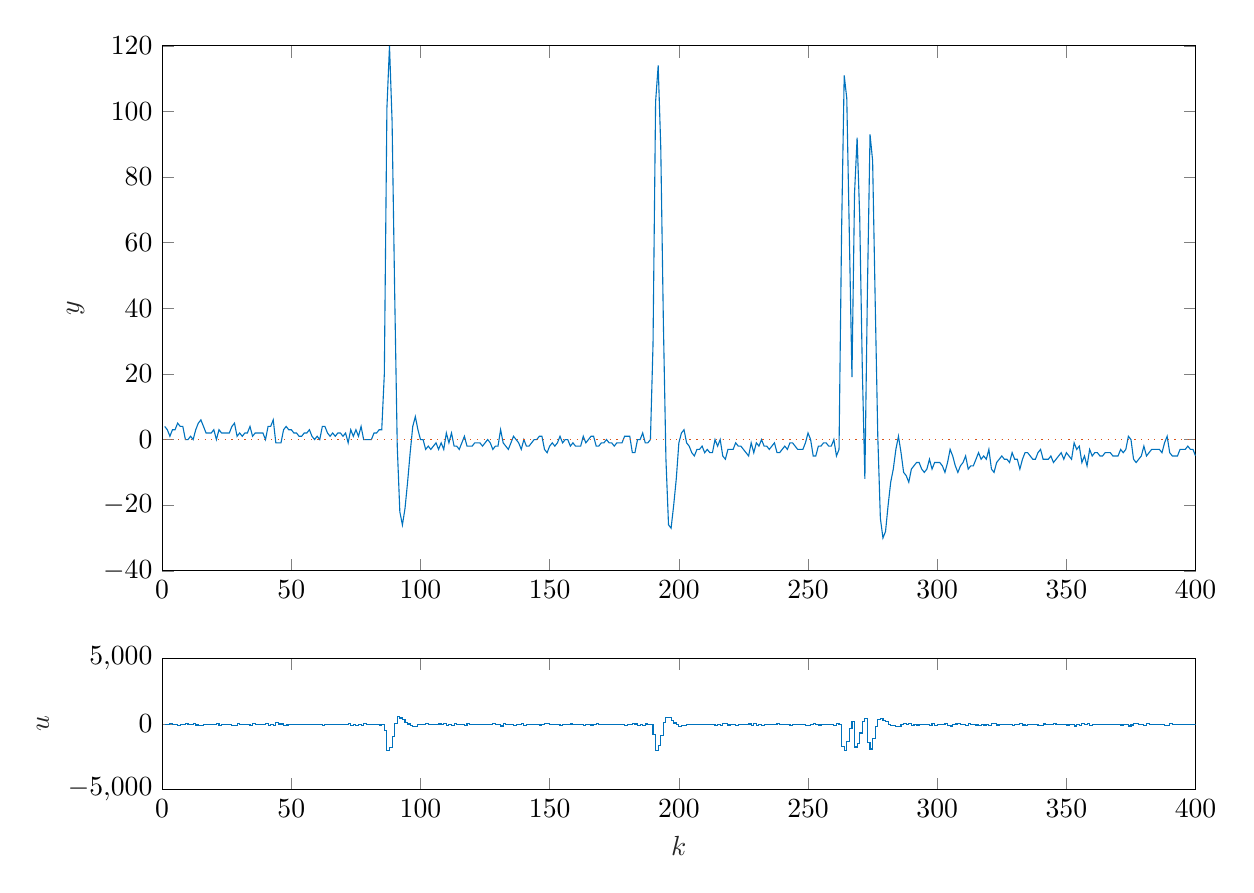
\begin{tikzpicture}

\begin{axis}[%
width=5.167in,
height=0.656in,
at={(0.646in,0.525in)},
scale only axis,
xmin=0,
xmax=400,
xtick={0,50,100,150,200,250,300,350,400},
xlabel style={font=\color{white!15!black}},
xlabel={$k$},
ymin=-5000,
ymax=5000,
ytick={-5000,0,5000},
ylabel style={font=\color{white!15!black}},
ylabel={$u$},
axis background/.style={fill=white}
]
\addplot[const plot, color=mycolor1, forget plot] table[row sep=crcr] {%
1	-62.88\\
2	-25.82\\
3	11.43\\
4	-63.82\\
5	-39.19\\
6	-89.69\\
7	-40.25\\
8	-53.25\\
9	46.5\\
10	-3.5\\
11	-28.57\\
12	8.87\\
13	-78.82\\
14	-91.82\\
15	-92.5\\
16	-30.63\\
17	-6\\
18	-31.25\\
19	-31.5\\
20	-56.82\\
21	30.5\\
22	-82.19\\
23	-20\\
24	-32.75\\
25	-33\\
26	-33.25\\
27	-83.63\\
28	-84.19\\
29	27.93\\
30	-47.25\\
31	-9.94\\
32	-47.63\\
33	-35.38\\
34	-85.75\\
35	13.93\\
36	-48.75\\
37	-36.5\\
38	-36.75\\
39	-37\\
40	12.87\\
41	-112.38\\
42	-62.88\\
43	-113.5\\
44	86.18\\
45	-1.19\\
46	-1.07\\
47	-101.19\\
48	-76.63\\
49	-39.57\\
50	-52.44\\
51	-27.75\\
52	-40.5\\
53	-15.69\\
54	-28.32\\
55	-53.5\\
56	-41.25\\
57	-66.57\\
58	-4.32\\
59	-4.38\\
60	-41.94\\
61	-4.5\\
62	-117.25\\
63	-67.75\\
64	-18.13\\
65	-18.32\\
66	-56\\
67	-18.69\\
68	-56.38\\
69	-44.13\\
70	-19.32\\
71	-57\\
72	30.43\\
73	-107.19\\
74	-7.44\\
75	-82.69\\
76	-7.94\\
77	-108.25\\
78	29\\
79	-21\\
80	-21\\
81	-21\\
82	-71.13\\
83	-46.38\\
84	-71.69\\
85	-59.57\\
86	-486\\
87	-2048\\
88	-1781.09\\
89	-982.15\\
90	21.47\\
91	543.79\\
92	457.79\\
93	310.79\\
94	138.72\\
95	3.35\\
96	-120.59\\
97	-208.09\\
98	-183.78\\
99	-46.9\\
100	-22.09\\
101	-59.59\\
102	15.6\\
103	-46.59\\
104	-8.78\\
105	-45.96\\
106	-58.28\\
107	4.47\\
108	-70.28\\
109	4.97\\
110	-144.96\\
111	-7.53\\
112	-120.09\\
113	17.41\\
114	-32.34\\
115	-7.03\\
116	-69.28\\
117	-94.28\\
118	5.79\\
119	-31.46\\
120	-31.21\\
121	-56.03\\
122	-43.4\\
123	-43.28\\
124	-18.09\\
125	-55.4\\
126	-67.84\\
127	-30.28\\
128	7.47\\
129	-42.21\\
130	-29.46\\
131	-154.53\\
132	7.85\\
133	-16.96\\
134	-4.15\\
135	-66.4\\
136	-91.4\\
137	-41.46\\
138	-28.9\\
139	8.85\\
140	-90.96\\
141	-3.34\\
142	-28.09\\
143	-52.9\\
144	-65.34\\
145	-52.84\\
146	-77.9\\
147	-65.53\\
148	34.6\\
149	10.04\\
150	-52.09\\
151	-51.9\\
152	-14.21\\
153	-51.53\\
154	-89.03\\
155	-14.03\\
156	-63.96\\
157	-51.46\\
158	-1.34\\
159	-51.15\\
160	-13.46\\
161	-25.71\\
162	-25.46\\
163	-100.4\\
164	-12.9\\
165	-62.84\\
166	-75.4\\
167	-63.03\\
168	12.04\\
169	-25.21\\
170	-50.03\\
171	-37.4\\
172	-62.34\\
173	-24.78\\
174	-37.15\\
175	-11.96\\
176	-49.28\\
177	-36.65\\
178	-36.53\\
179	-86.53\\
180	-61.65\\
181	-61.78\\
182	63.41\\
183	1.41\\
184	-98.34\\
185	-48.34\\
186	-98.46\\
187	1.47\\
188	-35.9\\
189	-60.84\\
190	-775.15\\
191	-2048\\
192	-1633.35\\
193	-883.54\\
194	121.15\\
195	506.78\\
196	483.78\\
197	262.09\\
198	77.53\\
199	-32.97\\
200	-207.16\\
201	-144.72\\
202	-132.54\\
203	-20.16\\
204	-44.97\\
205	-7.1\\
206	-6.54\\
207	-68.54\\
208	-43.16\\
209	-67.85\\
210	-4.97\\
211	-54.54\\
212	-16.6\\
213	-28.6\\
214	-128.35\\
215	-28.22\\
216	-103.1\\
217	47.21\\
218	10.4\\
219	-76.54\\
220	-38.66\\
221	-38.29\\
222	-88.04\\
223	-37.85\\
224	-50.1\\
225	-24.79\\
226	-11.85\\
227	1.21\\
228	-110.91\\
229	14.4\\
230	-97.79\\
231	-35.1\\
232	-97.47\\
233	-22.35\\
234	-47.1\\
235	-21.79\\
236	-58.97\\
237	-71.29\\
238	16.53\\
239	-20.47\\
240	-45.04\\
241	-57.22\\
242	-19.41\\
243	-81.66\\
244	-56.54\\
245	-31.35\\
246	-18.54\\
247	-30.66\\
248	-30.29\\
249	-80.04\\
250	-130.1\\
251	-42.72\\
252	57.59\\
253	-4.29\\
254	-78.85\\
255	-41.1\\
256	-65.91\\
257	-53.29\\
258	-28.1\\
259	-40.35\\
260	-90.22\\
261	60.09\\
262	-51.91\\
263	-1705.72\\
264	-2048\\
265	-1305.07\\
266	-352.94\\
267	191.99\\
268	-1751.38\\
269	-1486.82\\
270	-684.32\\
271	160.06\\
272	434.43\\
273	-1442.69\\
274	-1901.38\\
275	-1125.01\\
276	-157.94\\
277	326.87\\
278	440.81\\
279	281.68\\
280	160.31\\
281	-11.69\\
282	-84.63\\
283	-95.76\\
284	-195.01\\
285	-219.88\\
286	-44.69\\
287	43.68\\
288	-5.01\\
289	33.99\\
290	-89.63\\
291	-63.57\\
292	-75.13\\
293	-61.76\\
294	-10.76\\
295	-9.57\\
296	-45.88\\
297	-107.44\\
298	5.99\\
299	-80.51\\
300	-54.63\\
301	-53.76\\
302	-27.82\\
303	10.81\\
304	-88.13\\
305	-150.01\\
306	-49.51\\
307	1.31\\
308	14.93\\
309	-58.94\\
310	-58.01\\
311	-94.76\\
312	31.12\\
313	-42.82\\
314	-29.32\\
315	-78.44\\
316	-102.82\\
317	-27.19\\
318	-76.51\\
319	-38.32\\
320	-125.26\\
321	62.99\\
322	14.18\\
323	-72.26\\
324	-58.94\\
325	-70.76\\
326	-32.57\\
327	-44.32\\
328	-18.51\\
329	-105.32\\
330	-17.19\\
331	-41.44\\
332	34.49\\
333	-77.07\\
334	-88.94\\
335	-63.44\\
336	-37.88\\
337	-24.69\\
338	-36.44\\
339	-85.82\\
340	-85.38\\
341	2.68\\
342	-34.07\\
343	-33.32\\
344	-57.63\\
345	5.62\\
346	-43.57\\
347	-55.38\\
348	-67.32\\
349	-4.19\\
350	-78.57\\
351	-28.01\\
352	-14.82\\
353	-151.88\\
354	-39.13\\
355	-88.82\\
356	49.24\\
357	-62.51\\
358	38.31\\
359	-123.51\\
360	-10.51\\
361	-59.94\\
362	-46.94\\
363	-21.38\\
364	-33.26\\
365	-57.69\\
366	-44.69\\
367	-44.19\\
368	-18.63\\
369	-30.51\\
370	-29.88\\
371	-79.38\\
372	-28.94\\
373	-66.01\\
374	-153.38\\
375	-78.44\\
376	59.43\\
377	10.24\\
378	-26.44\\
379	-38.26\\
380	-100.32\\
381	12.62\\
382	-49.32\\
383	-61.38\\
384	-48.51\\
385	-48.13\\
386	-47.76\\
387	-22.32\\
388	-109.51\\
389	-122.01\\
390	28.18\\
391	-8.76\\
392	-20.63\\
393	-20.01\\
394	-69.51\\
395	-44.13\\
396	-43.76\\
397	-68.44\\
398	-30.63\\
399	-42.76\\
400	7.74\\
};
\end{axis}

\begin{axis}[%
width=5.167in,
height=2.625in,
at={(0.646in,1.619in)},
scale only axis,
xmin=0,
xmax=400,
xtick={0,50,100,150,200,250,300,350,400},
ymin=-40,
ymax=120,
ytick={-40,-20,0,20,40,60,80,100,120},
ylabel style={font=\color{white!15!black}},
ylabel={$y$},
axis background/.style={fill=white}
]
\addplot [color=mycolor1, forget plot]
  table[row sep=crcr]{%
1	4\\
2	3\\
3	1\\
4	3\\
5	3\\
6	5\\
7	4\\
8	4\\
9	0\\
10	0\\
11	1\\
12	0\\
13	3\\
14	5\\
15	6\\
16	4\\
17	2\\
18	2\\
19	2\\
20	3\\
21	0\\
22	3\\
23	2\\
24	2\\
25	2\\
26	2\\
27	4\\
28	5\\
29	1\\
30	2\\
31	1\\
32	2\\
33	2\\
34	4\\
35	1\\
36	2\\
37	2\\
38	2\\
39	2\\
40	0\\
41	4\\
42	4\\
43	6\\
44	-1\\
45	-1\\
46	-1\\
47	3\\
48	4\\
49	3\\
50	3\\
51	2\\
52	2\\
53	1\\
54	1\\
55	2\\
56	2\\
57	3\\
58	1\\
59	0\\
60	1\\
61	0\\
62	4\\
63	4\\
64	2\\
65	1\\
66	2\\
67	1\\
68	2\\
69	2\\
70	1\\
71	2\\
72	-1\\
73	3\\
74	1\\
75	3\\
76	1\\
77	4\\
78	0\\
79	0\\
80	0\\
81	0\\
82	2\\
83	2\\
84	3\\
85	3\\
86	20\\
87	101\\
88	120\\
89	97\\
90	45\\
91	-2\\
92	-22\\
93	-26\\
94	-21\\
95	-13\\
96	-4\\
97	4\\
98	7\\
99	3\\
100	0\\
101	0\\
102	-3\\
103	-2\\
104	-3\\
105	-2\\
106	-1\\
107	-3\\
108	-1\\
109	-3\\
110	2\\
111	-1\\
112	2\\
113	-2\\
114	-2\\
115	-3\\
116	-1\\
117	1\\
118	-2\\
119	-2\\
120	-2\\
121	-1\\
122	-1\\
123	-1\\
124	-2\\
125	-1\\
126	0\\
127	-1\\
128	-3\\
129	-2\\
130	-2\\
131	3\\
132	-1\\
133	-2\\
134	-3\\
135	-1\\
136	1\\
137	0\\
138	-1\\
139	-3\\
140	0\\
141	-2\\
142	-2\\
143	-1\\
144	0\\
145	0\\
146	1\\
147	1\\
148	-3\\
149	-4\\
150	-2\\
151	-1\\
152	-2\\
153	-1\\
154	1\\
155	-1\\
156	0\\
157	0\\
158	-2\\
159	-1\\
160	-2\\
161	-2\\
162	-2\\
163	1\\
164	-1\\
165	0\\
166	1\\
167	1\\
168	-2\\
169	-2\\
170	-1\\
171	-1\\
172	0\\
173	-1\\
174	-1\\
175	-2\\
176	-1\\
177	-1\\
178	-1\\
179	1\\
180	1\\
181	1\\
182	-4\\
183	-4\\
184	0\\
185	0\\
186	2\\
187	-1\\
188	-1\\
189	0\\
190	29\\
191	103\\
192	114\\
193	89\\
194	36\\
195	-6\\
196	-26\\
197	-27\\
198	-20\\
199	-12\\
200	-1\\
201	2\\
202	3\\
203	-1\\
204	-2\\
205	-4\\
206	-5\\
207	-3\\
208	-3\\
209	-2\\
210	-4\\
211	-3\\
212	-4\\
213	-4\\
214	0\\
215	-2\\
216	0\\
217	-5\\
218	-6\\
219	-3\\
220	-3\\
221	-3\\
222	-1\\
223	-2\\
224	-2\\
225	-3\\
226	-4\\
227	-5\\
228	-1\\
229	-4\\
230	-1\\
231	-2\\
232	0\\
233	-2\\
234	-2\\
235	-3\\
236	-2\\
237	-1\\
238	-4\\
239	-4\\
240	-3\\
241	-2\\
242	-3\\
243	-1\\
244	-1\\
245	-2\\
246	-3\\
247	-3\\
248	-3\\
249	-1\\
250	2\\
251	0\\
252	-5\\
253	-5\\
254	-2\\
255	-2\\
256	-1\\
257	-1\\
258	-2\\
259	-2\\
260	0\\
261	-5\\
262	-3\\
263	64\\
264	111\\
265	104\\
266	62\\
267	19\\
268	75\\
269	92\\
270	68\\
271	22\\
272	-12\\
273	46\\
274	93\\
275	85\\
276	42\\
277	1\\
278	-24\\
279	-30\\
280	-28\\
281	-20\\
282	-13\\
283	-9\\
284	-3\\
285	1\\
286	-4\\
287	-10\\
288	-11\\
289	-13\\
290	-9\\
291	-8\\
292	-7\\
293	-7\\
294	-9\\
295	-10\\
296	-9\\
297	-6\\
298	-9\\
299	-7\\
300	-7\\
301	-7\\
302	-8\\
303	-10\\
304	-7\\
305	-3\\
306	-5\\
307	-8\\
308	-10\\
309	-8\\
310	-7\\
311	-5\\
312	-9\\
313	-8\\
314	-8\\
315	-6\\
316	-4\\
317	-6\\
318	-5\\
319	-6\\
320	-3\\
321	-9\\
322	-10\\
323	-7\\
324	-6\\
325	-5\\
326	-6\\
327	-6\\
328	-7\\
329	-4\\
330	-6\\
331	-6\\
332	-9\\
333	-6\\
334	-4\\
335	-4\\
336	-5\\
337	-6\\
338	-6\\
339	-4\\
340	-3\\
341	-6\\
342	-6\\
343	-6\\
344	-5\\
345	-7\\
346	-6\\
347	-5\\
348	-4\\
349	-6\\
350	-4\\
351	-5\\
352	-6\\
353	-1\\
354	-3\\
355	-2\\
356	-7\\
357	-5\\
358	-8\\
359	-3\\
360	-5\\
361	-4\\
362	-4\\
363	-5\\
364	-5\\
365	-4\\
366	-4\\
367	-4\\
368	-5\\
369	-5\\
370	-5\\
371	-3\\
372	-4\\
373	-3\\
374	1\\
375	0\\
376	-6\\
377	-7\\
378	-6\\
379	-5\\
380	-2\\
381	-5\\
382	-4\\
383	-3\\
384	-3\\
385	-3\\
386	-3\\
387	-4\\
388	-1\\
389	1\\
390	-4\\
391	-5\\
392	-5\\
393	-5\\
394	-3\\
395	-3\\
396	-3\\
397	-2\\
398	-3\\
399	-3\\
400	-5\\
};
\addplot[const plot, color=mycolor2, dotted, forget plot] table[row sep=crcr] {%
1	0\\
2	0\\
3	0\\
4	0\\
5	0\\
6	0\\
7	0\\
8	0\\
9	0\\
10	0\\
11	0\\
12	0\\
13	0\\
14	0\\
15	0\\
16	0\\
17	0\\
18	0\\
19	0\\
20	0\\
21	0\\
22	0\\
23	0\\
24	0\\
25	0\\
26	0\\
27	0\\
28	0\\
29	0\\
30	0\\
31	0\\
32	0\\
33	0\\
34	0\\
35	0\\
36	0\\
37	0\\
38	0\\
39	0\\
40	0\\
41	0\\
42	0\\
43	0\\
44	0\\
45	0\\
46	0\\
47	0\\
48	0\\
49	0\\
50	0\\
51	0\\
52	0\\
53	0\\
54	0\\
55	0\\
56	0\\
57	0\\
58	0\\
59	0\\
60	0\\
61	0\\
62	0\\
63	0\\
64	0\\
65	0\\
66	0\\
67	0\\
68	0\\
69	0\\
70	0\\
71	0\\
72	0\\
73	0\\
74	0\\
75	0\\
76	0\\
77	0\\
78	0\\
79	0\\
80	0\\
81	0\\
82	0\\
83	0\\
84	0\\
85	0\\
86	0\\
87	0\\
88	0\\
89	0\\
90	0\\
91	0\\
92	0\\
93	0\\
94	0\\
95	0\\
96	0\\
97	0\\
98	0\\
99	0\\
100	0\\
101	0\\
102	0\\
103	0\\
104	0\\
105	0\\
106	0\\
107	0\\
108	0\\
109	0\\
110	0\\
111	0\\
112	0\\
113	0\\
114	0\\
115	0\\
116	0\\
117	0\\
118	0\\
119	0\\
120	0\\
121	0\\
122	0\\
123	0\\
124	0\\
125	0\\
126	0\\
127	0\\
128	0\\
129	0\\
130	0\\
131	0\\
132	0\\
133	0\\
134	0\\
135	0\\
136	0\\
137	0\\
138	0\\
139	0\\
140	0\\
141	0\\
142	0\\
143	0\\
144	0\\
145	0\\
146	0\\
147	0\\
148	0\\
149	0\\
150	0\\
151	0\\
152	0\\
153	0\\
154	0\\
155	0\\
156	0\\
157	0\\
158	0\\
159	0\\
160	0\\
161	0\\
162	0\\
163	0\\
164	0\\
165	0\\
166	0\\
167	0\\
168	0\\
169	0\\
170	0\\
171	0\\
172	0\\
173	0\\
174	0\\
175	0\\
176	0\\
177	0\\
178	0\\
179	0\\
180	0\\
181	0\\
182	0\\
183	0\\
184	0\\
185	0\\
186	0\\
187	0\\
188	0\\
189	0\\
190	0\\
191	0\\
192	0\\
193	0\\
194	0\\
195	0\\
196	0\\
197	0\\
198	0\\
199	0\\
200	0\\
201	0\\
202	0\\
203	0\\
204	0\\
205	0\\
206	0\\
207	0\\
208	0\\
209	0\\
210	0\\
211	0\\
212	0\\
213	0\\
214	0\\
215	0\\
216	0\\
217	0\\
218	0\\
219	0\\
220	0\\
221	0\\
222	0\\
223	0\\
224	0\\
225	0\\
226	0\\
227	0\\
228	0\\
229	0\\
230	0\\
231	0\\
232	0\\
233	0\\
234	0\\
235	0\\
236	0\\
237	0\\
238	0\\
239	0\\
240	0\\
241	0\\
242	0\\
243	0\\
244	0\\
245	0\\
246	0\\
247	0\\
248	0\\
249	0\\
250	0\\
251	0\\
252	0\\
253	0\\
254	0\\
255	0\\
256	0\\
257	0\\
258	0\\
259	0\\
260	0\\
261	0\\
262	0\\
263	0\\
264	0\\
265	0\\
266	0\\
267	0\\
268	0\\
269	0\\
270	0\\
271	0\\
272	0\\
273	0\\
274	0\\
275	0\\
276	0\\
277	0\\
278	0\\
279	0\\
280	0\\
281	0\\
282	0\\
283	0\\
284	0\\
285	0\\
286	0\\
287	0\\
288	0\\
289	0\\
290	0\\
291	0\\
292	0\\
293	0\\
294	0\\
295	0\\
296	0\\
297	0\\
298	0\\
299	0\\
300	0\\
301	0\\
302	0\\
303	0\\
304	0\\
305	0\\
306	0\\
307	0\\
308	0\\
309	0\\
310	0\\
311	0\\
312	0\\
313	0\\
314	0\\
315	0\\
316	0\\
317	0\\
318	0\\
319	0\\
320	0\\
321	0\\
322	0\\
323	0\\
324	0\\
325	0\\
326	0\\
327	0\\
328	0\\
329	0\\
330	0\\
331	0\\
332	0\\
333	0\\
334	0\\
335	0\\
336	0\\
337	0\\
338	0\\
339	0\\
340	0\\
341	0\\
342	0\\
343	0\\
344	0\\
345	0\\
346	0\\
347	0\\
348	0\\
349	0\\
350	0\\
351	0\\
352	0\\
353	0\\
354	0\\
355	0\\
356	0\\
357	0\\
358	0\\
359	0\\
360	0\\
361	0\\
362	0\\
363	0\\
364	0\\
365	0\\
366	0\\
367	0\\
368	0\\
369	0\\
370	0\\
371	0\\
372	0\\
373	0\\
374	0\\
375	0\\
376	0\\
377	0\\
378	0\\
379	0\\
380	0\\
381	0\\
382	0\\
383	0\\
384	0\\
385	0\\
386	0\\
387	0\\
388	0\\
389	0\\
390	0\\
391	0\\
392	0\\
393	0\\
394	0\\
395	0\\
396	0\\
397	0\\
398	0\\
399	0\\
400	0\\
};
\end{axis}
\end{tikzpicture}%
\end{figure}


\begin{figure}[H]
\centering
%err =1517632
\definecolor{mycolor1}{rgb}{0.00000,0.44700,0.74100}%
\definecolor{mycolor2}{rgb}{0.85000,0.32500,0.09800}%
%
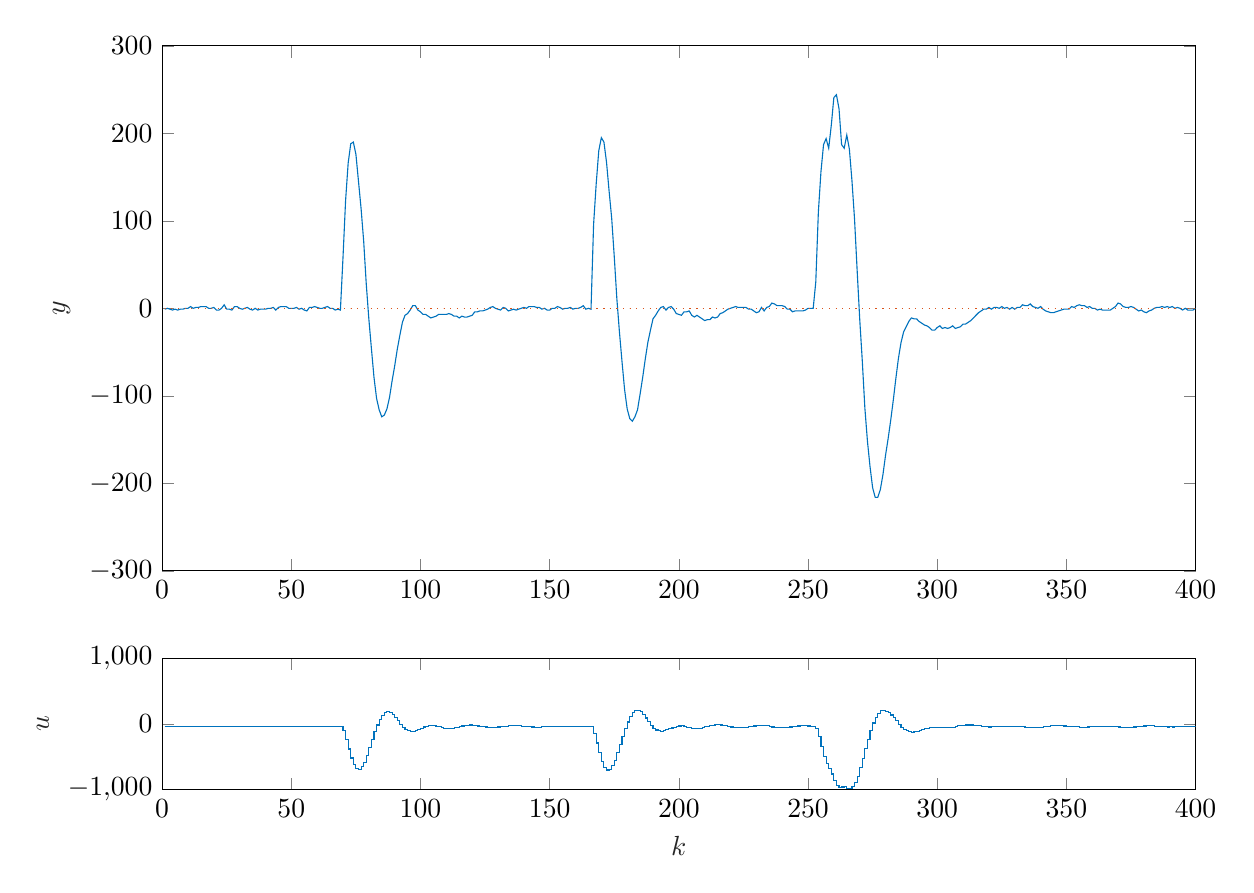
\begin{tikzpicture}

\begin{axis}[%
width=5.167in,
height=0.656in,
at={(0.646in,0.525in)},
scale only axis,
xmin=0,
xmax=400,
xtick={0,50,100,150,200,250,300,350,400},
xlabel style={font=\color{white!15!black}},
xlabel={$k$},
ymin=-1000,
ymax=1000,
ytick={-1000,0,1000},
ylabel style={font=\color{white!15!black}},
ylabel={$u$},
axis background/.style={fill=white}
]
\addplot[const plot, color=mycolor1, forget plot] table[row sep=crcr] {%
1	-37.5\\
2	-38.07\\
3	-37.4\\
4	-35.64\\
5	-35.5\\
6	-34.16\\
7	-34.05\\
8	-33.91\\
9	-35.02\\
10	-35.82\\
11	-38.84\\
12	-38.74\\
13	-39.69\\
14	-40.42\\
15	-42.08\\
16	-43.22\\
17	-44.11\\
18	-42.45\\
19	-41.17\\
20	-41.37\\
21	-37.94\\
22	-35.3\\
23	-35.82\\
24	-41.06\\
25	-39.24\\
26	-38.03\\
27	-36.07\\
28	-39.27\\
29	-41.58\\
30	-40.95\\
31	-39.4\\
32	-39.58\\
33	-40.85\\
34	-39.29\\
35	-36.78\\
36	-37.23\\
37	-35.26\\
38	-34.84\\
39	-34.54\\
40	-34.46\\
41	-35.63\\
42	-36.5\\
43	-38.34\\
44	-36.1\\
45	-37.99\\
46	-40.62\\
47	-42.5\\
48	-43.74\\
49	-42.39\\
50	-41.26\\
51	-40.26\\
52	-40.62\\
53	-38.39\\
54	-38.01\\
55	-35.59\\
56	-32.73\\
57	-35.32\\
58	-37.36\\
59	-40.15\\
60	-41.23\\
61	-40.95\\
62	-40.66\\
63	-41.42\\
64	-43.16\\
65	-42.01\\
66	-41.13\\
67	-38.1\\
68	-37.06\\
69	-35.01\\
70	-104.13\\
71	-233.14\\
72	-380.75\\
73	-517.91\\
74	-623.08\\
75	-683.34\\
76	-688.21\\
77	-652.32\\
78	-581.9\\
79	-475.76\\
80	-357.01\\
81	-238.24\\
82	-120.94\\
83	-14.79\\
84	70.77\\
85	136.44\\
86	175.91\\
87	190.3\\
88	180.23\\
89	146.91\\
90	101.92\\
91	49.19\\
92	-2.88\\
93	-50.99\\
94	-86.19\\
95	-103.41\\
96	-109.62\\
97	-109.88\\
98	-101.58\\
99	-83.29\\
100	-64\\
101	-45.06\\
102	-32.54\\
103	-24.54\\
104	-20.62\\
105	-23.57\\
106	-31.53\\
107	-43.13\\
108	-53.95\\
109	-62.34\\
110	-67.35\\
111	-69.8\\
112	-67\\
113	-58.86\\
114	-49.63\\
115	-38.05\\
116	-30.18\\
117	-22.6\\
118	-17.36\\
119	-15.7\\
120	-16.8\\
121	-23.62\\
122	-29.69\\
123	-35.86\\
124	-40.62\\
125	-44.87\\
126	-48.03\\
127	-51.24\\
128	-53.17\\
129	-50.6\\
130	-45.92\\
131	-39.72\\
132	-37.56\\
133	-34.24\\
134	-28.28\\
135	-25.61\\
136	-25.66\\
137	-25.56\\
138	-27.75\\
139	-31.51\\
140	-36.19\\
141	-38.89\\
142	-43.26\\
143	-46.33\\
144	-48.12\\
145	-47.56\\
146	-46.45\\
147	-42.58\\
148	-40.35\\
149	-36.14\\
150	-32.87\\
151	-32.99\\
152	-33.43\\
153	-36.53\\
154	-38.2\\
155	-37.44\\
156	-38.28\\
157	-39.01\\
158	-40.68\\
159	-39.59\\
160	-39.88\\
161	-40\\
162	-41.02\\
163	-43.81\\
164	-40.95\\
165	-39.8\\
166	-37.59\\
167	-150.19\\
168	-289.76\\
169	-439.23\\
170	-570.02\\
171	-661.88\\
172	-700.67\\
173	-686.82\\
174	-637.79\\
175	-550.61\\
176	-434.86\\
177	-312.3\\
178	-191.34\\
179	-73.54\\
180	30.81\\
181	113.01\\
182	170.86\\
183	200.81\\
184	207.1\\
185	185.57\\
186	144.66\\
187	90.93\\
188	32.92\\
189	-19.32\\
190	-64.35\\
191	-91.52\\
192	-105.55\\
193	-109.51\\
194	-103.7\\
195	-86.89\\
196	-72.64\\
197	-60.94\\
198	-48.23\\
199	-35.91\\
200	-29.75\\
201	-28.39\\
202	-36.67\\
203	-47.33\\
204	-59.38\\
205	-64.9\\
206	-66.27\\
207	-67.97\\
208	-64.14\\
209	-55.2\\
210	-42.74\\
211	-32.11\\
212	-22.21\\
213	-17.24\\
214	-12.58\\
215	-10.84\\
216	-15.26\\
217	-20.74\\
218	-28.24\\
219	-36.93\\
220	-44.81\\
221	-51.45\\
222	-56.54\\
223	-57.7\\
224	-56.8\\
225	-54.36\\
226	-50.78\\
227	-44.16\\
228	-38.23\\
229	-31.05\\
230	-23.39\\
231	-19.28\\
232	-23.08\\
233	-22.39\\
234	-27.93\\
235	-34.48\\
236	-44.76\\
237	-51.61\\
238	-54.24\\
239	-55.85\\
240	-56.45\\
241	-54.88\\
242	-49.41\\
243	-44.87\\
244	-37.6\\
245	-33.22\\
246	-29.9\\
247	-27.63\\
248	-26.53\\
249	-27.46\\
250	-31.01\\
251	-34.19\\
252	-36.87\\
253	-74.41\\
254	-197.1\\
255	-343.45\\
256	-489.38\\
257	-606.95\\
258	-680.29\\
259	-762.02\\
260	-857.5\\
261	-931.43\\
262	-971.2\\
263	-959.96\\
264	-954.94\\
265	-977.01\\
266	-983.07\\
267	-955.33\\
268	-895.47\\
269	-795.6\\
270	-668.08\\
271	-529.42\\
272	-375.85\\
273	-230.02\\
274	-99.51\\
275	15.16\\
276	104.97\\
277	166.34\\
278	200.26\\
279	208.86\\
280	195.57\\
281	171.16\\
282	137.41\\
283	95.83\\
284	48.09\\
285	-1.15\\
286	-46.51\\
287	-82.46\\
288	-104.79\\
289	-117.94\\
290	-123.02\\
291	-118.54\\
292	-110.8\\
293	-98.12\\
294	-85.2\\
295	-73.4\\
296	-64.5\\
297	-58.2\\
298	-52.26\\
299	-49.25\\
300	-52.32\\
301	-57.69\\
302	-57.74\\
303	-58.08\\
304	-54.82\\
305	-50.71\\
306	-47.26\\
307	-37.88\\
308	-29.44\\
309	-22.57\\
310	-19.14\\
311	-15.46\\
312	-14.35\\
313	-15\\
314	-18.22\\
315	-23.29\\
316	-29.42\\
317	-35.24\\
318	-40.6\\
319	-42.98\\
320	-45.42\\
321	-43.3\\
322	-42.67\\
323	-41.07\\
324	-37.89\\
325	-37.34\\
326	-34.48\\
327	-33.72\\
328	-31.2\\
329	-32.22\\
330	-31.34\\
331	-33.77\\
332	-36.42\\
333	-42.59\\
334	-46.39\\
335	-49.31\\
336	-53.8\\
337	-53.22\\
338	-51.14\\
339	-47.92\\
340	-47.43\\
341	-43.42\\
342	-37.96\\
343	-32.83\\
344	-28.04\\
345	-24.64\\
346	-23.59\\
347	-24.39\\
348	-26.55\\
349	-29.65\\
350	-32.15\\
351	-33.83\\
352	-38.39\\
353	-40.19\\
354	-43.44\\
355	-46.69\\
356	-47.58\\
357	-47.93\\
358	-45.53\\
359	-44.63\\
360	-41.46\\
361	-39.16\\
362	-35.31\\
363	-34.07\\
364	-32.36\\
365	-31.51\\
366	-31.23\\
367	-31.26\\
368	-33.84\\
369	-38.21\\
370	-46.15\\
371	-50.86\\
372	-50.66\\
373	-49\\
374	-47.32\\
375	-46.78\\
376	-44.99\\
377	-41.39\\
378	-36.62\\
379	-34.45\\
380	-30.7\\
381	-26.81\\
382	-26.48\\
383	-27.65\\
384	-31.19\\
385	-35.22\\
386	-38.41\\
387	-42\\
388	-43.21\\
389	-44.84\\
390	-44.49\\
391	-45.09\\
392	-43.03\\
393	-42.55\\
394	-40.84\\
395	-37.12\\
396	-36.69\\
397	-34.09\\
398	-32.27\\
399	-31.17\\
400	-33.04\\
};
\end{axis}

\begin{axis}[%
width=5.167in,
height=2.625in,
at={(0.646in,1.619in)},
scale only axis,
xmin=0,
xmax=400,
xtick={0,50,100,150,200,250,300,350,400},
ymin=-300,
ymax=300,
ytick={-300,-200,-100,0,100,200,300},
ylabel style={font=\color{white!15!black}},
ylabel={$y$},
axis background/.style={fill=white}
]
\addplot [color=mycolor1, forget plot]
  table[row sep=crcr]{%
1	-1\\
2	0\\
3	-1\\
4	-2\\
5	-1\\
6	-2\\
7	-1\\
8	-1\\
9	0\\
10	0\\
11	2\\
12	0\\
13	1\\
14	1\\
15	2\\
16	2\\
17	2\\
18	0\\
19	0\\
20	1\\
21	-2\\
22	-2\\
23	0\\
24	4\\
25	-1\\
26	-1\\
27	-2\\
28	2\\
29	2\\
30	0\\
31	-1\\
32	0\\
33	1\\
34	-1\\
35	-2\\
36	0\\
37	-2\\
38	-1\\
39	-1\\
40	-1\\
41	0\\
42	0\\
43	1\\
44	-2\\
45	1\\
46	2\\
47	2\\
48	2\\
49	0\\
50	0\\
51	0\\
52	1\\
53	-1\\
54	0\\
55	-2\\
56	-3\\
57	1\\
58	1\\
59	2\\
60	1\\
61	0\\
62	0\\
63	1\\
64	2\\
65	0\\
66	0\\
67	-2\\
68	-1\\
69	-2\\
70	58\\
71	123\\
72	166\\
73	188\\
74	190\\
75	176\\
76	145\\
77	114\\
78	77\\
79	28\\
80	-12\\
81	-46\\
82	-79\\
83	-103\\
84	-116\\
85	-124\\
86	-122\\
87	-115\\
88	-102\\
89	-83\\
90	-66\\
91	-47\\
92	-31\\
93	-16\\
94	-8\\
95	-6\\
96	-2\\
97	3\\
98	3\\
99	-2\\
100	-4\\
101	-7\\
102	-7\\
103	-9\\
104	-11\\
105	-10\\
106	-9\\
107	-7\\
108	-7\\
109	-7\\
110	-7\\
111	-6\\
112	-7\\
113	-9\\
114	-9\\
115	-11\\
116	-9\\
117	-10\\
118	-10\\
119	-9\\
120	-8\\
121	-4\\
122	-4\\
123	-3\\
124	-3\\
125	-2\\
126	-1\\
127	1\\
128	2\\
129	0\\
130	-1\\
131	-2\\
132	1\\
133	0\\
134	-3\\
135	-2\\
136	-1\\
137	-2\\
138	-1\\
139	0\\
140	1\\
141	0\\
142	2\\
143	2\\
144	2\\
145	1\\
146	1\\
147	-1\\
148	0\\
149	-2\\
150	-2\\
151	0\\
152	0\\
153	2\\
154	1\\
155	-1\\
156	0\\
157	0\\
158	1\\
159	-1\\
160	0\\
161	0\\
162	1\\
163	3\\
164	-1\\
165	0\\
166	-1\\
167	96\\
168	142\\
169	180\\
170	195\\
171	190\\
172	167\\
173	134\\
174	103\\
175	59\\
176	11\\
177	-27\\
178	-61\\
179	-93\\
180	-115\\
181	-126\\
182	-129\\
183	-124\\
184	-116\\
185	-98\\
186	-79\\
187	-58\\
188	-39\\
189	-25\\
190	-12\\
191	-8\\
192	-3\\
193	1\\
194	2\\
195	-2\\
196	1\\
197	2\\
198	-1\\
199	-6\\
200	-7\\
201	-8\\
202	-4\\
203	-4\\
204	-3\\
205	-8\\
206	-10\\
207	-8\\
208	-10\\
209	-12\\
210	-14\\
211	-13\\
212	-13\\
213	-10\\
214	-11\\
215	-10\\
216	-6\\
217	-5\\
218	-3\\
219	-1\\
220	0\\
221	1\\
222	2\\
223	1\\
224	1\\
225	1\\
226	1\\
227	-1\\
228	-1\\
229	-3\\
230	-5\\
231	-4\\
232	1\\
233	-3\\
234	1\\
235	2\\
236	6\\
237	5\\
238	3\\
239	3\\
240	3\\
241	2\\
242	-1\\
243	-1\\
244	-4\\
245	-3\\
246	-3\\
247	-3\\
248	-3\\
249	-2\\
250	0\\
251	0\\
252	0\\
253	30\\
254	110\\
255	156\\
256	187\\
257	194\\
258	183\\
259	209\\
260	241\\
261	244\\
262	228\\
263	187\\
264	183\\
265	198\\
266	182\\
267	146\\
268	102\\
269	44\\
270	-12\\
271	-60\\
272	-114\\
273	-152\\
274	-181\\
275	-205\\
276	-216\\
277	-216\\
278	-207\\
279	-190\\
280	-168\\
281	-149\\
282	-128\\
283	-105\\
284	-80\\
285	-57\\
286	-39\\
287	-27\\
288	-21\\
289	-15\\
290	-11\\
291	-12\\
292	-12\\
293	-15\\
294	-17\\
295	-19\\
296	-20\\
297	-22\\
298	-25\\
299	-25\\
300	-22\\
301	-20\\
302	-23\\
303	-22\\
304	-23\\
305	-22\\
306	-20\\
307	-23\\
308	-22\\
309	-21\\
310	-18\\
311	-18\\
312	-16\\
313	-14\\
314	-11\\
315	-8\\
316	-5\\
317	-3\\
318	-1\\
319	-1\\
320	1\\
321	-1\\
322	1\\
323	1\\
324	0\\
325	2\\
326	0\\
327	1\\
328	-1\\
329	1\\
330	-1\\
331	1\\
332	1\\
333	4\\
334	3\\
335	3\\
336	5\\
337	2\\
338	1\\
339	0\\
340	2\\
341	-1\\
342	-3\\
343	-4\\
344	-5\\
345	-5\\
346	-4\\
347	-3\\
348	-2\\
349	-1\\
350	-1\\
351	-1\\
352	2\\
353	1\\
354	3\\
355	4\\
356	3\\
357	3\\
358	1\\
359	2\\
360	0\\
361	0\\
362	-2\\
363	-1\\
364	-2\\
365	-2\\
366	-2\\
367	-2\\
368	0\\
369	2\\
370	6\\
371	5\\
372	2\\
373	1\\
374	1\\
375	2\\
376	1\\
377	-1\\
378	-3\\
379	-2\\
380	-4\\
381	-5\\
382	-3\\
383	-2\\
384	0\\
385	1\\
386	1\\
387	2\\
388	1\\
389	2\\
390	1\\
391	2\\
392	0\\
393	1\\
394	0\\
395	-2\\
396	0\\
397	-2\\
398	-2\\
399	-2\\
400	0\\
};
\addplot[const plot, color=mycolor2, dotted, forget plot] table[row sep=crcr] {%
1	0\\
2	0\\
3	0\\
4	0\\
5	0\\
6	0\\
7	0\\
8	0\\
9	0\\
10	0\\
11	0\\
12	0\\
13	0\\
14	0\\
15	0\\
16	0\\
17	0\\
18	0\\
19	0\\
20	0\\
21	0\\
22	0\\
23	0\\
24	0\\
25	0\\
26	0\\
27	0\\
28	0\\
29	0\\
30	0\\
31	0\\
32	0\\
33	0\\
34	0\\
35	0\\
36	0\\
37	0\\
38	0\\
39	0\\
40	0\\
41	0\\
42	0\\
43	0\\
44	0\\
45	0\\
46	0\\
47	0\\
48	0\\
49	0\\
50	0\\
51	0\\
52	0\\
53	0\\
54	0\\
55	0\\
56	0\\
57	0\\
58	0\\
59	0\\
60	0\\
61	0\\
62	0\\
63	0\\
64	0\\
65	0\\
66	0\\
67	0\\
68	0\\
69	0\\
70	0\\
71	0\\
72	0\\
73	0\\
74	0\\
75	0\\
76	0\\
77	0\\
78	0\\
79	0\\
80	0\\
81	0\\
82	0\\
83	0\\
84	0\\
85	0\\
86	0\\
87	0\\
88	0\\
89	0\\
90	0\\
91	0\\
92	0\\
93	0\\
94	0\\
95	0\\
96	0\\
97	0\\
98	0\\
99	0\\
100	0\\
101	0\\
102	0\\
103	0\\
104	0\\
105	0\\
106	0\\
107	0\\
108	0\\
109	0\\
110	0\\
111	0\\
112	0\\
113	0\\
114	0\\
115	0\\
116	0\\
117	0\\
118	0\\
119	0\\
120	0\\
121	0\\
122	0\\
123	0\\
124	0\\
125	0\\
126	0\\
127	0\\
128	0\\
129	0\\
130	0\\
131	0\\
132	0\\
133	0\\
134	0\\
135	0\\
136	0\\
137	0\\
138	0\\
139	0\\
140	0\\
141	0\\
142	0\\
143	0\\
144	0\\
145	0\\
146	0\\
147	0\\
148	0\\
149	0\\
150	0\\
151	0\\
152	0\\
153	0\\
154	0\\
155	0\\
156	0\\
157	0\\
158	0\\
159	0\\
160	0\\
161	0\\
162	0\\
163	0\\
164	0\\
165	0\\
166	0\\
167	0\\
168	0\\
169	0\\
170	0\\
171	0\\
172	0\\
173	0\\
174	0\\
175	0\\
176	0\\
177	0\\
178	0\\
179	0\\
180	0\\
181	0\\
182	0\\
183	0\\
184	0\\
185	0\\
186	0\\
187	0\\
188	0\\
189	0\\
190	0\\
191	0\\
192	0\\
193	0\\
194	0\\
195	0\\
196	0\\
197	0\\
198	0\\
199	0\\
200	0\\
201	0\\
202	0\\
203	0\\
204	0\\
205	0\\
206	0\\
207	0\\
208	0\\
209	0\\
210	0\\
211	0\\
212	0\\
213	0\\
214	0\\
215	0\\
216	0\\
217	0\\
218	0\\
219	0\\
220	0\\
221	0\\
222	0\\
223	0\\
224	0\\
225	0\\
226	0\\
227	0\\
228	0\\
229	0\\
230	0\\
231	0\\
232	0\\
233	0\\
234	0\\
235	0\\
236	0\\
237	0\\
238	0\\
239	0\\
240	0\\
241	0\\
242	0\\
243	0\\
244	0\\
245	0\\
246	0\\
247	0\\
248	0\\
249	0\\
250	0\\
251	0\\
252	0\\
253	0\\
254	0\\
255	0\\
256	0\\
257	0\\
258	0\\
259	0\\
260	0\\
261	0\\
262	0\\
263	0\\
264	0\\
265	0\\
266	0\\
267	0\\
268	0\\
269	0\\
270	0\\
271	0\\
272	0\\
273	0\\
274	0\\
275	0\\
276	0\\
277	0\\
278	0\\
279	0\\
280	0\\
281	0\\
282	0\\
283	0\\
284	0\\
285	0\\
286	0\\
287	0\\
288	0\\
289	0\\
290	0\\
291	0\\
292	0\\
293	0\\
294	0\\
295	0\\
296	0\\
297	0\\
298	0\\
299	0\\
300	0\\
301	0\\
302	0\\
303	0\\
304	0\\
305	0\\
306	0\\
307	0\\
308	0\\
309	0\\
310	0\\
311	0\\
312	0\\
313	0\\
314	0\\
315	0\\
316	0\\
317	0\\
318	0\\
319	0\\
320	0\\
321	0\\
322	0\\
323	0\\
324	0\\
325	0\\
326	0\\
327	0\\
328	0\\
329	0\\
330	0\\
331	0\\
332	0\\
333	0\\
334	0\\
335	0\\
336	0\\
337	0\\
338	0\\
339	0\\
340	0\\
341	0\\
342	0\\
343	0\\
344	0\\
345	0\\
346	0\\
347	0\\
348	0\\
349	0\\
350	0\\
351	0\\
352	0\\
353	0\\
354	0\\
355	0\\
356	0\\
357	0\\
358	0\\
359	0\\
360	0\\
361	0\\
362	0\\
363	0\\
364	0\\
365	0\\
366	0\\
367	0\\
368	0\\
369	0\\
370	0\\
371	0\\
372	0\\
373	0\\
374	0\\
375	0\\
376	0\\
377	0\\
378	0\\
379	0\\
380	0\\
381	0\\
382	0\\
383	0\\
384	0\\
385	0\\
386	0\\
387	0\\
388	0\\
389	0\\
390	0\\
391	0\\
392	0\\
393	0\\
394	0\\
395	0\\
396	0\\
397	0\\
398	0\\
399	0\\
400	0\\
};
\end{axis}
\end{tikzpicture}%
\end{figure}



\begin{equation}
\end{equation}


\begin{lstlisting}[style=Matlab-editor]
s = tf('s');

sys = K/((s*T1+1)*(s*T2+1))*exp(-Td*s);
% wartości T1, T2 oraz Td otrzymano podczas optymalizacji
% parametrów modelu wykorzystanego przy aproksymacji

pidtune(sys,'PID');
\end{lstlisting} 

